% Options for packages loaded elsewhere
\PassOptionsToPackage{unicode}{hyperref}
\PassOptionsToPackage{hyphens}{url}
%
\documentclass[
  12pt,
]{book}
\usepackage{lmodern}
\usepackage{amssymb,amsmath}
\usepackage{ifxetex,ifluatex}
\ifnum 0\ifxetex 1\fi\ifluatex 1\fi=0 % if pdftex
  \usepackage[T1]{fontenc}
  \usepackage[utf8]{inputenc}
  \usepackage{textcomp} % provide euro and other symbols
\else % if luatex or xetex
  \usepackage{unicode-math}
  \defaultfontfeatures{Scale=MatchLowercase}
  \defaultfontfeatures[\rmfamily]{Ligatures=TeX,Scale=1}
\fi
% Use upquote if available, for straight quotes in verbatim environments
\IfFileExists{upquote.sty}{\usepackage{upquote}}{}
\IfFileExists{microtype.sty}{% use microtype if available
  \usepackage[]{microtype}
  \UseMicrotypeSet[protrusion]{basicmath} % disable protrusion for tt fonts
}{}
\makeatletter
\@ifundefined{KOMAClassName}{% if non-KOMA class
  \IfFileExists{parskip.sty}{%
    \usepackage{parskip}
  }{% else
    \setlength{\parindent}{0pt}
    \setlength{\parskip}{6pt plus 2pt minus 1pt}}
}{% if KOMA class
  \KOMAoptions{parskip=half}}
\makeatother
\usepackage{xcolor}
\IfFileExists{xurl.sty}{\usepackage{xurl}}{} % add URL line breaks if available
\IfFileExists{bookmark.sty}{\usepackage{bookmark}}{\usepackage{hyperref}}
\hypersetup{
  pdftitle={How to fit an animal model},
  pdfauthor={Julien Martin},
  hidelinks,
  pdfcreator={LaTeX via pandoc}}
\urlstyle{same} % disable monospaced font for URLs
\usepackage{color}
\usepackage{fancyvrb}
\newcommand{\VerbBar}{|}
\newcommand{\VERB}{\Verb[commandchars=\\\{\}]}
\DefineVerbatimEnvironment{Highlighting}{Verbatim}{commandchars=\\\{\}}
% Add ',fontsize=\small' for more characters per line
\usepackage{framed}
\definecolor{shadecolor}{RGB}{248,248,248}
\newenvironment{Shaded}{\begin{snugshade}}{\end{snugshade}}
\newcommand{\AlertTok}[1]{\textcolor[rgb]{0.94,0.16,0.16}{#1}}
\newcommand{\AnnotationTok}[1]{\textcolor[rgb]{0.56,0.35,0.01}{\textbf{\textit{#1}}}}
\newcommand{\AttributeTok}[1]{\textcolor[rgb]{0.77,0.63,0.00}{#1}}
\newcommand{\BaseNTok}[1]{\textcolor[rgb]{0.00,0.00,0.81}{#1}}
\newcommand{\BuiltInTok}[1]{#1}
\newcommand{\CharTok}[1]{\textcolor[rgb]{0.31,0.60,0.02}{#1}}
\newcommand{\CommentTok}[1]{\textcolor[rgb]{0.56,0.35,0.01}{\textit{#1}}}
\newcommand{\CommentVarTok}[1]{\textcolor[rgb]{0.56,0.35,0.01}{\textbf{\textit{#1}}}}
\newcommand{\ConstantTok}[1]{\textcolor[rgb]{0.00,0.00,0.00}{#1}}
\newcommand{\ControlFlowTok}[1]{\textcolor[rgb]{0.13,0.29,0.53}{\textbf{#1}}}
\newcommand{\DataTypeTok}[1]{\textcolor[rgb]{0.13,0.29,0.53}{#1}}
\newcommand{\DecValTok}[1]{\textcolor[rgb]{0.00,0.00,0.81}{#1}}
\newcommand{\DocumentationTok}[1]{\textcolor[rgb]{0.56,0.35,0.01}{\textbf{\textit{#1}}}}
\newcommand{\ErrorTok}[1]{\textcolor[rgb]{0.64,0.00,0.00}{\textbf{#1}}}
\newcommand{\ExtensionTok}[1]{#1}
\newcommand{\FloatTok}[1]{\textcolor[rgb]{0.00,0.00,0.81}{#1}}
\newcommand{\FunctionTok}[1]{\textcolor[rgb]{0.00,0.00,0.00}{#1}}
\newcommand{\ImportTok}[1]{#1}
\newcommand{\InformationTok}[1]{\textcolor[rgb]{0.56,0.35,0.01}{\textbf{\textit{#1}}}}
\newcommand{\KeywordTok}[1]{\textcolor[rgb]{0.13,0.29,0.53}{\textbf{#1}}}
\newcommand{\NormalTok}[1]{#1}
\newcommand{\OperatorTok}[1]{\textcolor[rgb]{0.81,0.36,0.00}{\textbf{#1}}}
\newcommand{\OtherTok}[1]{\textcolor[rgb]{0.56,0.35,0.01}{#1}}
\newcommand{\PreprocessorTok}[1]{\textcolor[rgb]{0.56,0.35,0.01}{\textit{#1}}}
\newcommand{\RegionMarkerTok}[1]{#1}
\newcommand{\SpecialCharTok}[1]{\textcolor[rgb]{0.00,0.00,0.00}{#1}}
\newcommand{\SpecialStringTok}[1]{\textcolor[rgb]{0.31,0.60,0.02}{#1}}
\newcommand{\StringTok}[1]{\textcolor[rgb]{0.31,0.60,0.02}{#1}}
\newcommand{\VariableTok}[1]{\textcolor[rgb]{0.00,0.00,0.00}{#1}}
\newcommand{\VerbatimStringTok}[1]{\textcolor[rgb]{0.31,0.60,0.02}{#1}}
\newcommand{\WarningTok}[1]{\textcolor[rgb]{0.56,0.35,0.01}{\textbf{\textit{#1}}}}
\usepackage{longtable,booktabs}
% Correct order of tables after \paragraph or \subparagraph
\usepackage{etoolbox}
\makeatletter
\patchcmd\longtable{\par}{\if@noskipsec\mbox{}\fi\par}{}{}
\makeatother
% Allow footnotes in longtable head/foot
\IfFileExists{footnotehyper.sty}{\usepackage{footnotehyper}}{\usepackage{footnote}}
\makesavenoteenv{longtable}
\usepackage{graphicx}
\makeatletter
\def\maxwidth{\ifdim\Gin@nat@width>\linewidth\linewidth\else\Gin@nat@width\fi}
\def\maxheight{\ifdim\Gin@nat@height>\textheight\textheight\else\Gin@nat@height\fi}
\makeatother
% Scale images if necessary, so that they will not overflow the page
% margins by default, and it is still possible to overwrite the defaults
% using explicit options in \includegraphics[width, height, ...]{}
\setkeys{Gin}{width=\maxwidth,height=\maxheight,keepaspectratio}
% Set default figure placement to htbp
\makeatletter
\def\fps@figure{htbp}
\makeatother
\setlength{\emergencystretch}{3em} % prevent overfull lines
\providecommand{\tightlist}{%
  \setlength{\itemsep}{0pt}\setlength{\parskip}{0pt}}
\setcounter{secnumdepth}{5}
%\usepackage{booktabs}
\usepackage{ctable}
\usepackage{fancyhdr}
\usepackage{float}
\usepackage[margin=2cm]{geometry}

\floatplacement{figure}{H}

%\usepackage[sf,bf]{titlesec}

\hypersetup{colorlinks=true, urlcolor=blue}

\renewcommand{\chaptername}{Chapitre}
\renewcommand{\contentsname}{Table des Matières}
\renewcommand{\partname}{Partie}

\usepackage{framed,color}
\definecolor{incolor}{RGB}{240,240,240}
\definecolor{outcolor}{RGB}{248,248,248}

\renewcommand{\textfraction}{0.05}
\renewcommand{\topfraction}{0.8}
\renewcommand{\bottomfraction}{0.8}
\renewcommand{\floatpagefraction}{0.75}

%\renewenvironment{quote}{\begin{VF}}{\end{VF}}

\ifxetex
 \usepackage{letltxmacro}
 \setlength{\XeTeXLinkMargin}{1pt}
 \LetLtxMacro\SavedIncludeGraphics\includegraphics
 \def\includegraphics#1#{% #1 catches optional stuff (star/opt. arg.)
   \IncludeGraphicsAux{#1}%
 }%
 \newcommand*{\IncludeGraphicsAux}[2]{%
   \XeTeXLinkBox{%
     \SavedIncludeGraphics#1{#2}%
   }%
 }%
\fi

\makeatletter
\newenvironment{kframe}{%
\medskip{}
\setlength{\fboxsep}{.8em}
\def\at@end@of@kframe{}%
\ifinner\ifhmode%
 \def\at@end@of@kframe{\end{minipage}}%
 \begin{minipage}{\columnwidth}%
\fi\fi%
\def\FrameCommand##1{\hskip\@totalleftmargin \hskip-\fboxsep
\colorbox{incolor}{##1}\hskip-\fboxsep
    % There is no \\@totalrightmargin, so:
    \hskip-\linewidth \hskip-\@totalleftmargin \hskip\columnwidth}%
\MakeFramed {\advance\hsize-\width
  \@totalleftmargin\z@ \linewidth\hsize
  \@setminipage}}%
{\par\unskip\endMakeFramed%
\at@end@of@kframe}
\makeatother

\makeatletter
\@ifundefined{Shaded}{
}{\renewenvironment{Shaded}{\begin{kframe}}{\end{kframe}}}
\makeatother

% \let\oldverbatim\verbatim
% \renewenvironment{Shaded}{\vspace{0.2cm}\begin{kframe}}{\end{kframe}}
% \renewenvironment{verbatim}{\begin{shaded}\begin{oldverbatim}}{\end{oldverbatim}\end{shaded}}

\newenvironment{rmdblock}[1]
 {
 \begin{itemize}
 \renewcommand{\labelitemi}{
   \raisebox{-.7\height}[0pt][0pt]{
     {\setkeys{Gin}{width=3em,keepaspectratio}\includegraphics{images/#1}}
   }
 }
 \begin{kframe}
 \setlength{\fboxsep}{1em}
 \item
 }
 {
 \end{kframe}
 \end{itemize}
 }
\newenvironment{rmdnote}
  {\begin{rmdblock}{note}}
  {\end{rmdblock}}
\newenvironment{rmdcaution}
  {\begin{rmdblock}{caution}}
  {\end{rmdblock}}
\newenvironment{rmdimportant}
  {\begin{rmdblock}{important}}
  {\end{rmdblock}}
\newenvironment{rmdtip}
  {\begin{rmdblock}{tip}}
  {\end{rmdblock}}
\newenvironment{rmdwarning}
  {\begin{rmdblock}{warning}}
  {\end{rmdblock}}
\newenvironment{rmdcode}
  {\begin{rmdblock}{screen}}
  {\end{rmdblock}}

\usepackage{makeidx}
\makeindex

\urlstyle{tt}

\usepackage{amsthm}
\makeatletter
\def\thm@space@setup{%
  \thm@preskip=8pt plus 2pt minus 4pt
  \thm@postskip=\thm@preskip
}
\makeatother

% \frontmatter
\usepackage[]{natbib}
\bibliographystyle{apalike}

\title{How to fit an animal model}
\usepackage{etoolbox}
\makeatletter
\providecommand{\subtitle}[1]{% add subtitle to \maketitle
  \apptocmd{\@title}{\par {\large #1 \par}}{}{}
}
\makeatother
\subtitle{An ecologist guide}
\author{Julien Martin}
\date{23-11-2021}

\begin{document}
\maketitle

%\cleardoublepage\newpage\thispagestyle{empty}\null
%\cleardoublepage\newpage\thispagestyle{empty}\null
%\cleardoublepage\newpage
%\thispagestyle{empty}
%\begin{center}
%
\includegraphics{images/missing.png}
%\end{center}

%\setlength{\abovedisplayskip}{-5pt}
%\setlength{\abovedisplayshortskip}{-5pt}

{
\setcounter{tocdepth}{1}
\tableofcontents
}
\hypertarget{preface}{%
\chapter*{Preface}\label{preface}}
\addcontentsline{toc}{chapter}{Preface}

This book is a collection of tutorial from the excellent paper by \citep{wilson2010}.
Instead of just copy pasting the tutorial in a bookdown format, the tutorials have been updated to work with the newest version of the softwares and extended to present other softwares.
\textbf{However, this is still a work in progress.}

\begin{rmdwarning}
Do not take anything in this manual as gospel.
\end{rmdwarning}

\hypertarget{contributors}{%
\subsection*{Contributors}\label{contributors}}
\addcontentsline{toc}{subsection}{Contributors}

List of people who contributed to update and extend tutorials:

\begin{itemize}
\tightlist
\item
  Eric Postma
\item
  Julien Martin
\item
  Mathieu Videlier
\end{itemize}

\hypertarget{intro}{%
\chapter{Introduction}\label{intro}}

The book is provides a series of tutorials (and accompanying data files) to fit animal model in \texttt{R} using different packages (\texttt{ASReml-R}, \texttt{gremlin}, \texttt{MCMCglmm} and \texttt{brms}/\texttt{stan}) .
You will need to carefully follow the instructions below to first download the data files and second install the R packages.
Before beginning the tutorial, we assume the reader has successfully installed the chosen R package on their computer and has saved the required data files to an appropriate directory from which they will be read.
Full instructions for how to do this are provided with software distributions.

To work though the different tutorial I would recommend to create a folder where you will save your different \texttt{R} scripts for the tutorials.

\hypertarget{data}{%
\section{Data}\label{data}}

\hypertarget{data-files}{%
\subsection{Data files}\label{data-files}}

You will need to download 3 data files for the tutorial in \texttt{R}:

\begin{itemize}
\tightlist
\item
  gryphon.csv: data on gryphon birth weight
\item
  gryphonRM.csv: data
\item
  gryphonped.csv
\end{itemize}

In addition, some models presented in the tutorials can take a while to run (sometimes \textgreater{} 1 hour), thus we are also providing model the model outputs to allow you continue the tutorial without waiting for the model to run.

The files are available \href{https://github.com/JulienGAMartin/wam_tuto/tree/master/data}{here}

I recommend to save the data and Rdata files in a subfolder \texttt{data} in the folder you will use as your working directory for R and where you will save your R scripts. It should be noted that the tutorial are using this structure to read or save data.

\hypertarget{notes-on-data-and-pedigree}{%
\subsection{Notes on data and pedigree}\label{notes-on-data-and-pedigree}}

It is always important to take time to think carefully about the strengths and potential limitations of your pedigree information before embarking on quantitative genetic analyses. Pedigree Viewer, written by Brian Kinghorn, is an extremely useful application for visualizing pedigrees, and can be downloaded from: \url{http://www-personal.une.edu.au/~bkinghor/pedigree.htm}. \texttt{Pedantics} an R package written by Michael Morrissey and distributed through CRAN (\url{http://cran.r-project.org/}) can also be used for this and offers some nice additional features for visualizing pedigree structures and generating associated statistics. Before you begin running through the tutorials, we advise taking a moment to look at the pedigree files provided with them using Pedigree Viewer or Pedantics.

\hypertarget{r}{%
\section{R}\label{r}}

You should check that you have the most current version of R and R packages. You can check the number of the current version on CRAN. If you need to update (or install) R packages, use \texttt{install.packages()} and follow the prompted instructions.

\hypertarget{r-packages}{%
\subsection{R packages}\label{r-packages}}

\hypertarget{asreml-r}{%
\subsubsection{asreml-r}\label{asreml-r}}

ASReml-R is commercial software published by VSN international (\url{http://www.vsni.co.uk/software/asreml/}). This package is not free and requires a key access
Additional information and guide can be find in the Asreml-R manual: (\url{https://asreml.kb.vsni.co.uk/wp-content/uploads/sites/3/2018/02/ASReml-R-Reference-Manual-4.pdf})

\hypertarget{gremlin}{%
\subsubsection{gremlin}\label{gremlin}}

\texttt{gremlin} is a little monster appearing if you feed a mugwai after midnight. It is also a great and promising software to fit mixed models using a frequentist approach.

\hypertarget{mcmcglmm}{%
\subsubsection{MCMCglmm}\label{mcmcglmm}}

\texttt{MCMCglmm} is an R package for Bayesian mixed model analysis written by Jarrod Hadfield. It is a freeware distributed through CRAN (\url{http://cran.r-project.org/}). Information and guide about the package can be find in the user manual and vignettes (\url{http://cran.r-project.org/web/packages/MCMCglmm/index.html}).
Reference: \citep[\citet{R-MCMCglmm}]{MCMCglmm2010}.

This module provides some information that applies to MCMCglmm-based analyses in general, but that will not be included in other tutorials.
Most importantly, this applies to some of the simplest ways of determining the performance of a run using MCMCglmm, i.e., verification of the validity of of the posterior distribution.
This tutorial is not a substitute for working through the MCMCglmm course notes, which is available from CRAN (the Comprehensive R ArchiveNetwork, \url{http://cran.r-project.org/}, or can be accessed in R using the command vignette(``CourseNotes'',``MCMCglmm'')).
These tutorials do not introduce one of the main advantages of using MCMCglmm for analyses of data from natural populations -the ability to properly model non-normal responses.
These capabilities are introduced in the documentation that is distributed with MCMCglmm, and available from CRAN.

\hypertarget{brms}{%
\subsubsection{brms}\label{brms}}

\texttt{brms} provides an interface to fit Bayesian generalized multivariate (non-)linear multilevel models using \texttt{Stan}, which is a C++ package for obtaining full Bayesian inference (see \url{https://mc-stan.org/}).
The formula syntax is an extended version of the syntax applied in the `lme4' package to provide a familiar and simple interface for performing regression analyses.

It should be noted that if \texttt{brms} is able to fit animal model the parametrization used is not the most efficient and can take quite longer than using a different parametrization directly in \texttt{stan}.

\hypertarget{univariate-animal-model}{%
\chapter{Univariate animal model}\label{univariate-animal-model}}

This tutorial will demonstrate how to run a univariate animal model to estimate genetic variance in birth weight in the mighty gryphons.

\hypertarget{scenario-and-data}{%
\section{Scenario and data}\label{scenario-and-data}}

\hypertarget{scenario}{%
\subsection{Scenario}\label{scenario}}

In a population of gryphons there is strong positive selection on birth weight with heavier born individuals having, on average higher fitness. To find out whether increased birth weight will evolve in response to the selection, and if so how quickly, we want to estimate the heritability of birth weight.

\hypertarget{data-files-1}{%
\subsection{Data files}\label{data-files-1}}

Open \texttt{gryphonped.csv} and \texttt{gryphon.csv} in your text editor. The structure and contents of these files is fairly self-explanatory. The pedigree file \texttt{gryphonped.csv} contains three columns containing unique IDs that correspond to each animal, its father, and its mother. Note that this is a multigenerational pedigree, with the earliest generation (for which parentage information is necessarily missing) at the beginning of the file. For later-born individuals maternal identities are all known but paternity information is incomplete (a common situation in real world applications).
The phenotype data, as well as additional factors and covariates that we may wish to include in our model are contained in \texttt{gryphon.csv}. Columns correspond to individual identity (\texttt{animal}), maternal identity (\texttt{mother}), year of birth (\texttt{byear}), sex (\texttt{sex}, where \texttt{1} is female and \texttt{2} is male), birth weight (\texttt{bwt}), and tarsus length (\texttt{tarsus}). Each row of the data file contains a record for a different offspring individual. Note that all individuals included in the data file must be included as offspring in the pedigree file.

We can read teh data file, using \texttt{read.csv()} which consider by default that \texttt{NA} is the symbol for missing values and that the first line of the file contains the column headers.

It is a good idea to make sure that all variables are correctly assigned as numeric or factors:

\begin{Shaded}
\begin{Highlighting}[]
\NormalTok{gryphon}\OperatorTok{$}\NormalTok{animal \textless{}{-}}\StringTok{ }\KeywordTok{as.factor}\NormalTok{(gryphon}\OperatorTok{$}\NormalTok{animal)}
\NormalTok{gryphon}\OperatorTok{$}\NormalTok{mother \textless{}{-}}\StringTok{ }\KeywordTok{as.factor}\NormalTok{(gryphon}\OperatorTok{$}\NormalTok{mother)}
\NormalTok{gryphon}\OperatorTok{$}\NormalTok{byear \textless{}{-}}\StringTok{ }\KeywordTok{as.factor}\NormalTok{(gryphon}\OperatorTok{$}\NormalTok{byear)}
\NormalTok{gryphon}\OperatorTok{$}\NormalTok{sex \textless{}{-}}\StringTok{ }\KeywordTok{as.factor}\NormalTok{(gryphon}\OperatorTok{$}\NormalTok{sex)}
\NormalTok{gryphon}\OperatorTok{$}\NormalTok{bwt \textless{}{-}}\StringTok{ }\KeywordTok{as.numeric}\NormalTok{(gryphon}\OperatorTok{$}\NormalTok{bwt)}
\NormalTok{gryphon}\OperatorTok{$}\NormalTok{tarsus \textless{}{-}}\StringTok{ }\KeywordTok{as.numeric}\NormalTok{(gryphon}\OperatorTok{$}\NormalTok{tarsus)}
\end{Highlighting}
\end{Shaded}

Similarly we can read in the pedigree file, using \texttt{read.csv()} which consider by default that \texttt{NA} is the symbol for missing values and that the first line of the file contains the column headers.

\begin{verbatim}
## 'data.frame':    1309 obs. of  3 variables:
##  $ id    : int  1306 1304 1298 1293 1290 1288 1284 1283 1282 1278 ...
##  $ father: int  NA NA NA NA NA NA NA NA NA NA ...
##  $ mother: int  NA NA NA NA NA NA NA NA NA NA ...
\end{verbatim}

\begin{Shaded}
\begin{Highlighting}[]
\NormalTok{gryphonped}\OperatorTok{$}\NormalTok{id \textless{}{-}}\StringTok{ }\KeywordTok{as.factor}\NormalTok{(gryphonped}\OperatorTok{$}\NormalTok{id)}
\NormalTok{gryphonped}\OperatorTok{$}\NormalTok{father \textless{}{-}}\StringTok{ }\KeywordTok{as.factor}\NormalTok{(gryphonped}\OperatorTok{$}\NormalTok{father)}
\NormalTok{gryphonped}\OperatorTok{$}\NormalTok{mother \textless{}{-}}\StringTok{ }\KeywordTok{as.factor}\NormalTok{(gryphonped}\OperatorTok{$}\NormalTok{mother)}
\end{Highlighting}
\end{Shaded}

Now that we have imported the data and the pedigree file, we are ready to fit an animal model.

\hypertarget{asreml-r-1}{%
\section{Asreml-R}\label{asreml-r-1}}

\hypertarget{running-the-model}{%
\subsection{Running the model}\label{running-the-model}}

First we need to load the \texttt{asreml} library:

\begin{Shaded}
\begin{Highlighting}[]
\KeywordTok{library}\NormalTok{(asreml)}
\end{Highlighting}
\end{Shaded}

\begin{verbatim}
## Loading required package: Matrix
\end{verbatim}

\begin{verbatim}
## Online License checked out Tue Nov 23 22:10:39 2021
\end{verbatim}

To be able to fit an animal model, Asreml-r needs (the inverse of) the relationship matrix using the ainverse function:

\begin{Shaded}
\begin{Highlighting}[]
\NormalTok{ainv \textless{}{-}}\StringTok{ }\KeywordTok{ainverse}\NormalTok{(gryphonped)}
\end{Highlighting}
\end{Shaded}

We are now ready to specify our first model:

\begin{Shaded}
\begin{Highlighting}[]
\NormalTok{model1 \textless{}{-}}\StringTok{ }\KeywordTok{asreml}\NormalTok{(}
  \DataTypeTok{fixed =}\NormalTok{ bwt }\OperatorTok{\textasciitilde{}}\StringTok{ }\DecValTok{1}\NormalTok{, }\DataTypeTok{random =} \OperatorTok{\textasciitilde{}}\StringTok{ }\KeywordTok{vm}\NormalTok{(animal, ainv),}
  \DataTypeTok{residual =} \OperatorTok{\textasciitilde{}}\StringTok{ }\KeywordTok{idv}\NormalTok{(units),}
  \DataTypeTok{data =}\NormalTok{ gryphon,}
  \DataTypeTok{na.action =} \KeywordTok{na.method}\NormalTok{(}\DataTypeTok{x =} \StringTok{"omit"}\NormalTok{, }\DataTypeTok{y =} \StringTok{"omit"}\NormalTok{)}
\NormalTok{)}
\end{Highlighting}
\end{Shaded}

\begin{verbatim}
## Online License checked out Tue Nov 23 22:10:39 2021
## Model fitted using the sigma parameterization.
## ASReml 4.1.0 Tue Nov 23 22:10:39 2021
##           LogLik        Sigma2     DF     wall    cpu
##  1     -4128.454           1.0    853 22:10:39    0.0
##  2     -3284.272           1.0    853 22:10:39    0.0
##  3     -2354.992           1.0    853 22:10:39    0.0
##  4     -1710.357           1.0    853 22:10:39    0.0
##  5     -1363.555           1.0    853 22:10:39    0.0
##  6     -1263.516           1.0    853 22:10:39    0.0
##  7     -1247.854           1.0    853 22:10:39    0.0
##  8     -1247.185           1.0    853 22:10:39    0.0
##  9     -1247.183           1.0    853 22:10:39    0.0
\end{verbatim}

In this model, \texttt{bwt} is the response variable and the only fixed effect is the mean (the intercept, denoted as \texttt{1}). The only random effect we have fitted is \texttt{animal}, which will provide an estimate of \(V_A\). Our random \texttt{animal} effect is connected to the inverse related matrix \texttt{ainv} which integrate the relativeness or pedigree information.\\
\texttt{data=} specifies the name of the dataframe that contains our variables. Finally, we tell \texttt{asreml()} what to when it encounters \texttt{NA}s in either the dependent or predictor variables (in this case we choose to remove the records). If you use the argument ``include'' instead of ``omit'', model will keep the NA. With x=``include'', the model will exchange \texttt{NA} with 0. Be careful you need to standardize your trait so the mean will be equal to 0, if not estimates (including covariance in multivariate models) could be strongly biased due to the the missing values. y=``include'' will exchange \texttt{NA} with a factor labeled \texttt{mv} which will be included in the sparse equation. For more details see Asreml-R manual.

A note of the specification of the structure of the residuals: This simple univariate model will run fine without \texttt{residual=\textasciitilde{}idv(units)}. However, if you are going to use \texttt{vpredict()} to calculate the heritability (see below), not specifying the residuals in this way will result in a standard error for the heritability that is incorrect.

Any model has assumption which need to be checked. The model can be plot which help visualizing the distribution of the model residual and check the different assumptions.

\begin{Shaded}
\begin{Highlighting}[]
\KeywordTok{plot}\NormalTok{(model1)}
\end{Highlighting}
\end{Shaded}

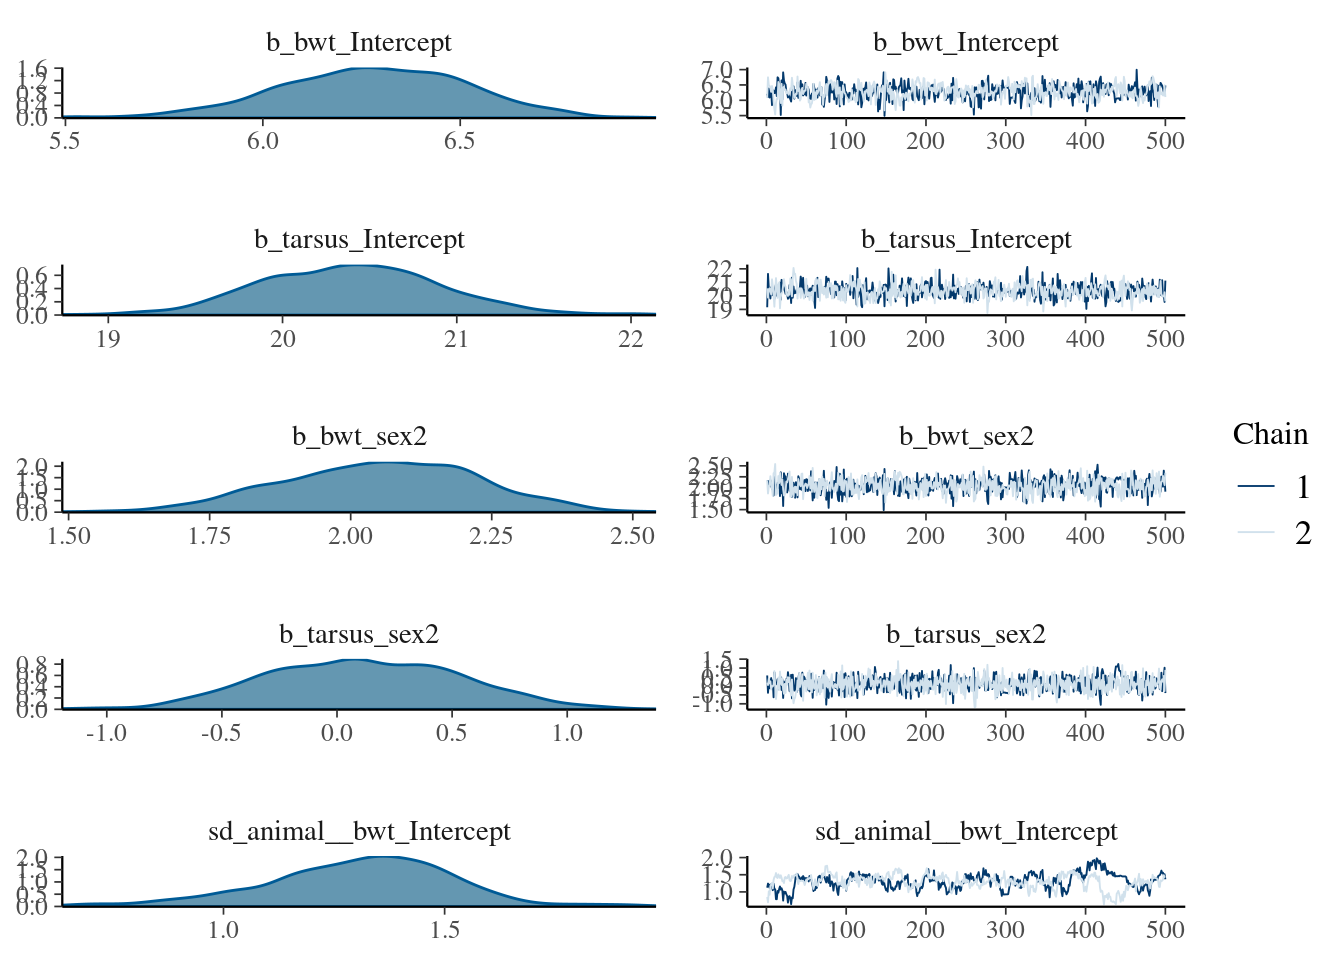
\includegraphics{wam_tuto_files/figure-latex/unnamed-chunk-10-1.pdf}

To see the estimates for the variance components, we run:

\begin{Shaded}
\begin{Highlighting}[]
\KeywordTok{summary}\NormalTok{(model1)}\OperatorTok{$}\NormalTok{varcomp}
\end{Highlighting}
\end{Shaded}

\begin{verbatim}
##                  component std.error  z.ratio bound %ch
## vm(animal, ainv)  3.395398 0.6349915 5.347154     P   0
## units!units       3.828602 0.5185919 7.382687     P   0
## units!R           1.000000        NA       NA     F   0
\end{verbatim}

We fitted a single random effect so we partitioned the phenotypic variance into two components. The \texttt{vm(animal,\ ainv)} variance component is \(V_A\) and is estimated as 3.4. Given that the ratio of \(V_A\) to its standard error (\texttt{z.ratio}) is considerably larger than 2 (\emph{i.e.} the parameter estimate is more than 2 SEs from zero), this looks likely to be significant. The \texttt{units!units} component refers to the residual variance \(V_R\), and \texttt{units\$R} should be ignored. If you don't include \texttt{residual=\textasciitilde{}idv(units)}in your model specification, \texttt{units\$R} will provide you with the residual variance.

\hypertarget{estimating-heritability}{%
\subsection{Estimating heritability}\label{estimating-heritability}}

We can calculate the \(h^2\) of birth weight from the components above since \(h^2 = V_A/V_P = V_A/(V_A+V_R)\). Thus according to this model, \(h^2\) = 3.4 / (3.4 + 3.83) = 0.47.

Alternatively we can use the \texttt{vpredict()} function to calculate \(h^2\) and its standard error. \texttt{vpredict()}function has two structures, first the model used (here \texttt{model1}) and then the estimate name with its associated equation. The equation used different \texttt{V} and their associated numbers depend of the order of the different random and residual effects included in the model.

\begin{Shaded}
\begin{Highlighting}[]
\KeywordTok{vpredict}\NormalTok{(model1, h2.bwt }\OperatorTok{\textasciitilde{}}\StringTok{ }\NormalTok{V1 }\OperatorTok{/}\StringTok{ }\NormalTok{(V1 }\OperatorTok{+}\StringTok{ }\NormalTok{V2))}
\end{Highlighting}
\end{Shaded}

\begin{verbatim}
##         Estimate         SE
## h2.bwt 0.4700163 0.07650881
\end{verbatim}

\hypertarget{adding-fixed-effects}{%
\subsection{Adding fixed effects}\label{adding-fixed-effects}}

To add fixed effects to a univariate model, we simply modify the model statement. For example, we might know (or suspect) that birth weight is a sexually dimorphic trait and therefore fit in the model.

\begin{Shaded}
\begin{Highlighting}[]
\NormalTok{model2 \textless{}{-}}\StringTok{ }\KeywordTok{asreml}\NormalTok{(}
  \DataTypeTok{fixed =}\NormalTok{ bwt }\OperatorTok{\textasciitilde{}}\StringTok{ }\DecValTok{1} \OperatorTok{+}\StringTok{ }\NormalTok{sex,}
  \DataTypeTok{random =} \OperatorTok{\textasciitilde{}}\StringTok{ }\KeywordTok{vm}\NormalTok{(animal, ainv),}
  \DataTypeTok{residual =} \OperatorTok{\textasciitilde{}}\StringTok{ }\KeywordTok{idv}\NormalTok{(units),}
  \DataTypeTok{data =}\NormalTok{ gryphon,}
  \DataTypeTok{na.action =} \KeywordTok{na.method}\NormalTok{(}\DataTypeTok{x =} \StringTok{"omit"}\NormalTok{, }\DataTypeTok{y =} \StringTok{"omit"}\NormalTok{)}
\NormalTok{)}
\end{Highlighting}
\end{Shaded}

\begin{verbatim}
## Model fitted using the sigma parameterization.
## ASReml 4.1.0 Tue Nov 23 22:10:40 2021
##           LogLik        Sigma2     DF     wall    cpu
##  1     -3364.126           1.0    852 22:10:40    0.0
##  2     -2702.117           1.0    852 22:10:40    0.0
##  3     -1978.916           1.0    852 22:10:40    0.0
##  4     -1487.834           1.0    852 22:10:40    0.0
##  5     -1236.350           1.0    852 22:10:40    0.0
##  6     -1172.771           1.0    852 22:10:40    0.0
##  7     -1165.270           1.0    852 22:10:40    0.0
##  8     -1165.093           1.0    852 22:10:40    0.0
##  9     -1165.093           1.0    852 22:10:40    0.0
\end{verbatim}

Now we can look at the fixed effects parameters and assess their significance with a conditional Wald F-test:

\begin{Shaded}
\begin{Highlighting}[]
\KeywordTok{summary}\NormalTok{(model2, }\DataTypeTok{coef =} \OtherTok{TRUE}\NormalTok{)}\OperatorTok{$}\NormalTok{coef.fixed}
\KeywordTok{wald.asreml}\NormalTok{(model2, }\DataTypeTok{ssType =} \StringTok{"conditional"}\NormalTok{, }\DataTypeTok{denDF =} \StringTok{"numeric"}\NormalTok{)}
\end{Highlighting}
\end{Shaded}

\begin{verbatim}
##             solution std error  z.ratio
## sex_1       0.000000        NA       NA
## sex_2       2.206996 0.1619974 13.62365
## (Intercept) 6.058669 0.1718244 35.26082
\end{verbatim}

\begin{verbatim}
## Model fitted using the sigma parameterization.
\end{verbatim}

\begin{verbatim}
## Warning in asreml(fixed = bwt ~ 1 + sex, random = ~vm(animal, ainv), residual =
## ~idv(units), : Algebraic derivatives for denominator df not available.
\end{verbatim}

\begin{verbatim}
## ASReml 4.1.0 Tue Nov 23 22:10:40 2021
##           LogLik        Sigma2     DF     wall    cpu
##  1     -1165.093           1.0    852 22:10:40    0.0
##  2     -1165.093           1.0    852 22:10:40    0.0
## Calculating denominator DF
\end{verbatim}

The very small probability (\texttt{Pr}) in the Wald test above shows that \texttt{sex} is a highly significant fixed effect, and from the parameter estimates (\texttt{summary(model2,coef=T)\$coef.fixed}) we can see that the average male (sex 2) is 2.2 kg (\(\pm\) 0.16 SE) heavier than the average female (sex 1). However, when we look at the variance components in the model including \texttt{sex} as a fixed effect, we see that they have changed slightly from the previous model:

\begin{Shaded}
\begin{Highlighting}[]
\KeywordTok{summary}\NormalTok{(model2)}\OperatorTok{$}\NormalTok{varcomp}
\end{Highlighting}
\end{Shaded}

\begin{verbatim}
##                  component std.error  z.ratio bound %ch
## vm(animal, ainv)  3.060441 0.5243571 5.836558     P   0
## units!units       2.938412 0.4161473 7.060991     P   0
## units!R           1.000000        NA       NA     F   0
\end{verbatim}

In fact since \texttt{sex} effects were previously contributing to the residual variance of the model, our estimate of \(V_R\) (denoted \texttt{units!R} in the output) is now slightly lower than before. This has an important consequence for estimating heritability since if we calculate \(V_P\) as \(V_A\)+\(V_R\) then as we include fixed effects we will soak up more residual variance driving \(V_P\). Assuming that \(V_A\) is more or less unaffected by the fixed effects fitted then as \(V_P\) goes down we expect our estimate of \(h^2\) will go up:

\begin{Shaded}
\begin{Highlighting}[]
\NormalTok{(h2}\FloatTok{.1}\NormalTok{ \textless{}{-}}\StringTok{ }\KeywordTok{vpredict}\NormalTok{(model1, h2.bwt }\OperatorTok{\textasciitilde{}}\StringTok{ }\NormalTok{V1 }\OperatorTok{/}\StringTok{ }\NormalTok{(V1 }\OperatorTok{+}\StringTok{ }\NormalTok{V2)))}
\end{Highlighting}
\end{Shaded}

\begin{verbatim}
##         Estimate         SE
## h2.bwt 0.4700163 0.07650881
\end{verbatim}

\begin{Shaded}
\begin{Highlighting}[]
\NormalTok{(h2}\FloatTok{.2}\NormalTok{ \textless{}{-}}\StringTok{ }\KeywordTok{vpredict}\NormalTok{(model2, h2.bwt }\OperatorTok{\textasciitilde{}}\StringTok{ }\NormalTok{V1 }\OperatorTok{/}\StringTok{ }\NormalTok{(V1 }\OperatorTok{+}\StringTok{ }\NormalTok{V2)))}
\end{Highlighting}
\end{Shaded}

\begin{verbatim}
##        Estimate         SE
## h2.bwt 0.510171 0.07432388
\end{verbatim}

Here \(h^2\) has increased slightly from 0.47 to 0.51. Which is the better estimate? It depends on what your question is. The first is an estimate of the proportion of variance in birth weight explained by additive effects, the latter is an estimate of the proportion of variance in birth weight \emph{after conditioning on sex} that is explained by additive effects.

An important piece of advice, each researcher should be consistent in how they name their estimates and always correctly describe which estimates they are using conditional or not (to avoid any confusion).

\hypertarget{adding-random-effects}{%
\subsection{Adding random effects}\label{adding-random-effects}}

This is done by simply modifying the model statement in the same way. For instance fitting

\begin{Shaded}
\begin{Highlighting}[]
\NormalTok{model3 \textless{}{-}}\StringTok{ }\KeywordTok{asreml}\NormalTok{(}
  \DataTypeTok{fixed =}\NormalTok{ bwt }\OperatorTok{\textasciitilde{}}\StringTok{ }\DecValTok{1} \OperatorTok{+}\StringTok{ }\NormalTok{sex,}
  \DataTypeTok{random =} \OperatorTok{\textasciitilde{}}\StringTok{ }\KeywordTok{vm}\NormalTok{(animal, ainv) }\OperatorTok{+}\StringTok{ }\NormalTok{byear,}
  \DataTypeTok{residual =} \OperatorTok{\textasciitilde{}}\StringTok{ }\KeywordTok{idv}\NormalTok{(units),}
  \DataTypeTok{data =}\NormalTok{ gryphon,}
  \DataTypeTok{na.action =} \KeywordTok{na.method}\NormalTok{(}\DataTypeTok{x =} \StringTok{"omit"}\NormalTok{, }\DataTypeTok{y =} \StringTok{"omit"}\NormalTok{)}
\NormalTok{)}
\end{Highlighting}
\end{Shaded}

\begin{verbatim}
## Model fitted using the sigma parameterization.
## ASReml 4.1.0 Tue Nov 23 22:10:40 2021
##           LogLik        Sigma2     DF     wall    cpu
##  1     -2742.658           1.0    852 22:10:41    0.0
##  2     -2237.268           1.0    852 22:10:41    0.0
##  3     -1690.453           1.0    852 22:10:41    0.0
##  4     -1328.910           1.0    852 22:10:41    0.0
##  5     -1154.597           1.0    852 22:10:41    0.0
##  6     -1116.992           1.0    852 22:10:41    0.0
##  7     -1113.809           1.0    852 22:10:41    0.0
##  8     -1113.772           1.0    852 22:10:41    0.0
##  9     -1113.772           1.0    852 22:10:41    0.0
\end{verbatim}

\begin{Shaded}
\begin{Highlighting}[]
\KeywordTok{summary}\NormalTok{(model3)}\OperatorTok{$}\NormalTok{varcomp}
\end{Highlighting}
\end{Shaded}

\begin{verbatim}
##                  component std.error  z.ratio bound %ch
## byear            0.8862604 0.2695918 3.287416     P   0
## vm(animal, ainv) 2.7068665 0.4422140 6.121169     P   0
## units!units      2.3092415 0.3451025 6.691466     P   0
## units!R          1.0000000        NA       NA     F   0
\end{verbatim}

\begin{Shaded}
\begin{Highlighting}[]
\NormalTok{(h2}\FloatTok{.3}\NormalTok{ \textless{}{-}}\StringTok{ }\KeywordTok{vpredict}\NormalTok{(model3, h2.bwt }\OperatorTok{\textasciitilde{}}\StringTok{ }\NormalTok{V1 }\OperatorTok{/}\StringTok{ }\NormalTok{(V1 }\OperatorTok{+}\StringTok{ }\NormalTok{V2 }\OperatorTok{+}\StringTok{ }\NormalTok{V3)))}
\end{Highlighting}
\end{Shaded}

\begin{verbatim}
##         Estimate         SE
## h2.bwt 0.1501533 0.03960814
\end{verbatim}

Here the variance in \texttt{bwt} explained by \texttt{byear} is 0.886 and, based on the \texttt{z.ratio}, appears to be significant (\textgreater2). Thus we would conclude that year-to-year variation (\emph{e.g.}, in weather, resource abundance) contributes to \(V_P\). Note that although \(V_A\) has changed somewhat, as most of what is now partitioned as a birth year effect was previously partitioned as \(V_R\). Thus what we have really done here is to partition environmental effects into those arising from year-to-year differences versus everything else, and we do not really expect much change in \(h^2\) (since now \(h^2 = V_A/ (V_A+V_{BY}+V_R)\)).

However, we get a somewhat different result if we also add a random effect of \texttt{mother} to test for maternal effects:

\begin{Shaded}
\begin{Highlighting}[]
\NormalTok{model4 \textless{}{-}}\StringTok{ }\KeywordTok{asreml}\NormalTok{(}
  \DataTypeTok{fixed =}\NormalTok{ bwt }\OperatorTok{\textasciitilde{}}\StringTok{ }\DecValTok{1} \OperatorTok{+}\StringTok{ }\NormalTok{sex,}
  \DataTypeTok{random =} \OperatorTok{\textasciitilde{}}\StringTok{ }\KeywordTok{vm}\NormalTok{(animal, ainv) }\OperatorTok{+}\StringTok{ }\NormalTok{byear }\OperatorTok{+}\StringTok{ }\NormalTok{mother,}
  \DataTypeTok{residual =} \OperatorTok{\textasciitilde{}}\StringTok{ }\KeywordTok{idv}\NormalTok{(units),}
  \DataTypeTok{data =}\NormalTok{ gryphon,}
  \DataTypeTok{na.action =} \KeywordTok{na.method}\NormalTok{(}\DataTypeTok{x =} \StringTok{"omit"}\NormalTok{, }\DataTypeTok{y =} \StringTok{"omit"}\NormalTok{)}
\NormalTok{)}
\end{Highlighting}
\end{Shaded}

\begin{verbatim}
## Model fitted using the sigma parameterization.
## ASReml 4.1.0 Tue Nov 23 22:10:41 2021
##           LogLik        Sigma2     DF     wall    cpu
##  1     -2033.178           1.0    852 22:10:41    0.0
##  2     -1723.734           1.0    852 22:10:41    0.0
##  3     -1396.354           1.0    852 22:10:41    0.0
##  4     -1193.012           1.0    852 22:10:41    0.0
##  5     -1107.946           1.0    852 22:10:41    0.0
##  6     -1095.327           1.0    852 22:10:41    0.0
##  7     -1094.816           1.0    852 22:10:41    0.0
##  8     -1094.815           1.0    852 22:10:41    0.0
\end{verbatim}

\begin{Shaded}
\begin{Highlighting}[]
\KeywordTok{summary}\NormalTok{(model4)}\OperatorTok{$}\NormalTok{varcomp}
\end{Highlighting}
\end{Shaded}

\begin{verbatim}
##                  component std.error  z.ratio bound %ch
## byear            0.8820313 0.2632455 3.350604     P   0
## mother           1.1184698 0.2386239 4.687167     P   0
## vm(animal, ainv) 2.2985320 0.4962496 4.631806     P   0
## units!units      1.6290034 0.3714154 4.385934     P   0
## units!R          1.0000000        NA       NA     F   0
\end{verbatim}

\begin{Shaded}
\begin{Highlighting}[]
\NormalTok{(h2}\FloatTok{.4}\NormalTok{ \textless{}{-}}\StringTok{ }\KeywordTok{vpredict}\NormalTok{(model4, h2.bwt }\OperatorTok{\textasciitilde{}}\StringTok{ }\NormalTok{V1 }\OperatorTok{/}\StringTok{ }\NormalTok{(V1 }\OperatorTok{+}\StringTok{ }\NormalTok{V2 }\OperatorTok{+}\StringTok{ }\NormalTok{V3 }\OperatorTok{+}\StringTok{ }\NormalTok{V4)))}
\end{Highlighting}
\end{Shaded}

\begin{verbatim}
##         Estimate         SE
## h2.bwt 0.1487898 0.03861552
\end{verbatim}

Here partitioning of significant maternal variance has resulted in a further decrease in \(V_R\) but also a decrease in \(V_A\). The latter is because maternal effects of the sort we simulated (fixed differences between mothers) will have the consequence of increasing similarity among maternal siblings. Consequently they can look very much like additive genetic effects and if present, but unmodelled, represent a type of ``common environment effect'' that can - and will - cause upward bias in \(V_A\) and so \(h^2\).
The ``common environment'' can be conceived as the indissociable sum of the maternal additive genetic effect (such as loci affecting milk production) and the maternal environment or permanent environment (such as litter or nest environment created or modified by the mother).

\hypertarget{testing-significance-of-random-effects}{%
\subsection{Testing significance of random effects}\label{testing-significance-of-random-effects}}

An important point to note in this tutorial is that while the \texttt{z.ratio} (\texttt{component}/\texttt{std.error}) reported is a good indicator of likely statistical significance (\textgreater1.96?), the standard errors are approximate and are not recommended for formal hypothesis testing. A better approach is to use likelihood-ratio tests (LRT).

For example, to test the significance of maternal effects we could compare models with and without the inclusion of maternal identity as a random effect and compare the final log-likelihoods of these models.

\begin{Shaded}
\begin{Highlighting}[]
\NormalTok{model4}\OperatorTok{$}\NormalTok{loglik}
\end{Highlighting}
\end{Shaded}

\begin{verbatim}
## [1] -1094.815
\end{verbatim}

shows that the model including maternal identity has a log-likelihood of -1094.815, and

\begin{Shaded}
\begin{Highlighting}[]
\NormalTok{model3}\OperatorTok{$}\NormalTok{loglik}
\end{Highlighting}
\end{Shaded}

\begin{verbatim}
## [1] -1113.772
\end{verbatim}

shows that the model excluding maternal identity has a log-likelihood of -1113.772.

A test statistic equal to twice the absolute difference in these log-likelihoods is assumed to be distributed as Chi square with \texttt{one} degree of freedom (one term of difference between the two models). In this case we would conclude that the maternal effects are highly significant since:
2 \(\times\) (-1094.8145793 - -1113.7719147) equals 37.9146708, and the p-value that comes with this is:

\begin{Shaded}
\begin{Highlighting}[]
\DecValTok{1} \OperatorTok{{-}}\StringTok{ }\KeywordTok{pchisq}\NormalTok{(}\DecValTok{2} \OperatorTok{*}\StringTok{ }\NormalTok{(model4}\OperatorTok{$}\NormalTok{loglik }\OperatorTok{{-}}\StringTok{ }\NormalTok{model3}\OperatorTok{$}\NormalTok{loglik), }\DecValTok{1}\NormalTok{)}
\end{Highlighting}
\end{Shaded}

\begin{verbatim}
## [1] 7.390738e-10
\end{verbatim}

As P \textless{} 0.0001 we would therefore conclude that the additional of maternal identity as a random effect significantly improves the fit of the model, given an increase in log-likelihood of approximately 19.

\hypertarget{further-partitioning-the-variance}{%
\subsection{Further partitioning the variance}\label{further-partitioning-the-variance}}

A population can be further fragmented into different groups or categories (such as females and males, juveniles and adults or treated and untreated). Some scientific questions require further and deeper analysis of the variance.
To avoid multiple model (one for each group), we can directly partition the variance between groups in a unique model. In addition, by doing so, we can also test if the variance are different between groups.

As example, we decide to take the model4 and partition its additive genetic variance and residual variance by sex. It is possible to further partition the other random effects but it will complexify the animal model and requires sufficient sample size.\\
First, the dataset needs to be order by group (here sex).

\begin{Shaded}
\begin{Highlighting}[]
\NormalTok{gryphon \textless{}{-}}\StringTok{ }\NormalTok{gryphon[}\KeywordTok{order}\NormalTok{(gryphon}\OperatorTok{$}\NormalTok{sex), ]}

\NormalTok{model\_SEX \textless{}{-}}\StringTok{ }\KeywordTok{asreml}\NormalTok{(}
  \DataTypeTok{fixed =}\NormalTok{ bwt }\OperatorTok{\textasciitilde{}}\StringTok{ }\DecValTok{1} \OperatorTok{+}\StringTok{ }\NormalTok{sex,}
  \DataTypeTok{random =} \OperatorTok{\textasciitilde{}}\StringTok{ }\KeywordTok{at}\NormalTok{(sex)}\OperatorTok{:}\KeywordTok{vm}\NormalTok{(animal, ainv) }\OperatorTok{+}\StringTok{ }\NormalTok{byear }\OperatorTok{+}\StringTok{ }\NormalTok{mother,}
  \DataTypeTok{residual =} \OperatorTok{\textasciitilde{}}\StringTok{ }\KeywordTok{dsum}\NormalTok{(}\OperatorTok{\textasciitilde{}}\StringTok{ }\NormalTok{units }\OperatorTok{|}\StringTok{ }\NormalTok{sex),}
  \DataTypeTok{data =}\NormalTok{ gryphon,}
  \DataTypeTok{na.action =} \KeywordTok{na.method}\NormalTok{(}\DataTypeTok{x =} \StringTok{"omit"}\NormalTok{, }\DataTypeTok{y =} \StringTok{"omit"}\NormalTok{)}
\NormalTok{)}
\end{Highlighting}
\end{Shaded}

\begin{verbatim}
## Multi-section model using the sigma parameterization.
## ASReml 4.1.0 Tue Nov 23 22:10:41 2021
##           LogLik        Sigma2     DF     wall    cpu
##  1     -1142.164           1.0    852 22:10:41    0.0
##  2     -1126.308           1.0    852 22:10:41    0.0
##  3     -1111.536           1.0    852 22:10:41    0.0
##  4     -1105.383           1.0    852 22:10:41    0.0
##  5     -1104.375           1.0    852 22:10:41    0.0
##  6     -1104.364           1.0    852 22:10:41    0.0
\end{verbatim}

To partition variance, two distinct function are requires \texttt{at()} at the random level, and \texttt{dsum()} at the residual level.

\begin{Shaded}
\begin{Highlighting}[]
\KeywordTok{summary}\NormalTok{(model\_SEX)}\OperatorTok{$}\NormalTok{varcomp}
\end{Highlighting}
\end{Shaded}

\begin{verbatim}
##                             component std.error  z.ratio bound %ch
## byear                       0.9001595 0.2690012 3.346303     P 0.0
## mother                      1.3396184 0.2663118 5.030263     P 0.0
## at(sex, 1):vm(animal, ainv) 1.4372390 0.6514306 2.206281     P 0.1
## at(sex, 2):vm(animal, ainv) 1.9861434 0.9974302 1.991261     P 0.3
## sex_1!R                     2.1706213 0.5542492 3.916327     P 0.0
## sex_2!R                     1.7112948 0.8246188 2.075256     P 0.3
\end{verbatim}

\begin{Shaded}
\begin{Highlighting}[]
\NormalTok{(h2.F \textless{}{-}}\StringTok{ }\KeywordTok{vpredict}\NormalTok{(model\_SEX, h2.bwt }\OperatorTok{\textasciitilde{}}\StringTok{ }\NormalTok{V3 }\OperatorTok{/}\StringTok{ }\NormalTok{(V1 }\OperatorTok{+}\StringTok{ }\NormalTok{V2 }\OperatorTok{+}\StringTok{ }\NormalTok{V3 }\OperatorTok{+}\StringTok{ }\NormalTok{V5)))}
\end{Highlighting}
\end{Shaded}

\begin{verbatim}
##         Estimate        SE
## h2.bwt 0.2457811 0.1070794
\end{verbatim}

\begin{Shaded}
\begin{Highlighting}[]
\NormalTok{(h2.M \textless{}{-}}\StringTok{ }\KeywordTok{vpredict}\NormalTok{(model\_SEX, h2.bwt }\OperatorTok{\textasciitilde{}}\StringTok{ }\NormalTok{V4 }\OperatorTok{/}\StringTok{ }\NormalTok{(V1 }\OperatorTok{+}\StringTok{ }\NormalTok{V2 }\OperatorTok{+}\StringTok{ }\NormalTok{V4 }\OperatorTok{+}\StringTok{ }\NormalTok{V6)))}
\end{Highlighting}
\end{Shaded}

\begin{verbatim}
##         Estimate        SE
## h2.bwt 0.3345244 0.1619218
\end{verbatim}

By partitioning the additive genetic variance and the residual variance, the model estimates the \(V_A\) and \(V_R\) for each group (sex). Doing so, we can calculate the \(h^2\) for each group (sex).

To test if the variance are different between groups, we can compare the model partitioned \texttt{model\_SEX} and the previous model without the partitioning \texttt{model4} in a likelihood ratio test (LRT) with 2 degrees of freedom since models have two components of variance of difference.

\begin{Shaded}
\begin{Highlighting}[]
\NormalTok{model\_SEX}\OperatorTok{$}\NormalTok{loglik}
\end{Highlighting}
\end{Shaded}

\begin{verbatim}
## [1] -1104.364
\end{verbatim}

\begin{Shaded}
\begin{Highlighting}[]
\NormalTok{model4}\OperatorTok{$}\NormalTok{loglik}
\end{Highlighting}
\end{Shaded}

\begin{verbatim}
## [1] -1094.815
\end{verbatim}

\begin{Shaded}
\begin{Highlighting}[]
\DecValTok{1} \OperatorTok{{-}}\StringTok{ }\KeywordTok{pchisq}\NormalTok{(}\DecValTok{2} \OperatorTok{*}\StringTok{ }\NormalTok{(model\_SEX}\OperatorTok{$}\NormalTok{loglik }\OperatorTok{{-}}\StringTok{ }\NormalTok{model4}\OperatorTok{$}\NormalTok{loglik), }\DecValTok{2}\NormalTok{)}
\end{Highlighting}
\end{Shaded}

\begin{verbatim}
## [1] 1
\end{verbatim}

Here, we can see the point estimates of \(h^2\) seems to differ between sexes (0.25 and 0.33), but their SE overlaps.
LRT give more information and showed that partitioning the variance and the residual between group (sex) did not improved the fit of the model and so their variance are not significantly different.

\hypertarget{modification-of-model-parameter}{%
\subsection{Modification of model parameter}\label{modification-of-model-parameter}}

Variance represents the deviation of the distribution and it expected to be a positive values.
Due to a lack of power, a structural problem in the dataset or a very low variance, Asreml-r often fixes the variance to a boundary \texttt{B} instead of a positive value \texttt{P}. When it is happen, it is generally a good idea to examine it.

To examine the boundary effect, we can exploit an alternative model where the model allowed a unstructured parameter for variance of interest or the entire variance matrix. For this example: we allowed the model to estimate any values (so allowing possible negative values of estimates) for the random and residual matrix.
First, we create a temporary model \texttt{model.temp} with the exact structure to modify.

\begin{Shaded}
\begin{Highlighting}[]
\NormalTok{model.temp \textless{}{-}}\StringTok{ }\KeywordTok{asreml}\NormalTok{(}
  \DataTypeTok{fixed =}\NormalTok{ bwt }\OperatorTok{\textasciitilde{}}\StringTok{ }\DecValTok{1}\NormalTok{,}
  \DataTypeTok{random =} \OperatorTok{\textasciitilde{}}\StringTok{ }\KeywordTok{vm}\NormalTok{(animal, ainv) }\OperatorTok{+}\StringTok{ }\NormalTok{byear }\OperatorTok{+}\StringTok{ }\NormalTok{mother,}
  \DataTypeTok{residual =} \OperatorTok{\textasciitilde{}}\StringTok{ }\KeywordTok{idv}\NormalTok{(units),}
  \DataTypeTok{data =}\NormalTok{ gryphon,}
  \DataTypeTok{na.action =} \KeywordTok{na.method}\NormalTok{(}\DataTypeTok{x =} \StringTok{"omit"}\NormalTok{, }\DataTypeTok{y =} \StringTok{"omit"}\NormalTok{),}
  \DataTypeTok{start.values =}\NormalTok{ T}
\NormalTok{)}
\NormalTok{G.temp \textless{}{-}}\StringTok{ }\NormalTok{model.temp}\OperatorTok{$}\NormalTok{vparameters[(}\DecValTok{1}\OperatorTok{:}\DecValTok{3}\NormalTok{), ]}
\NormalTok{G.temp}\OperatorTok{$}\NormalTok{Constraint \textless{}{-}}\StringTok{ "U"}
\NormalTok{R.temp \textless{}{-}}\StringTok{ }\NormalTok{model.temp}\OperatorTok{$}\NormalTok{vparameters[}\OperatorTok{{-}}\NormalTok{(}\DecValTok{1}\OperatorTok{:}\DecValTok{3}\NormalTok{), ]}
\NormalTok{R.temp}\OperatorTok{$}\NormalTok{Constraint[}\DecValTok{2}\NormalTok{] \textless{}{-}}\StringTok{ "U"}
\end{Highlighting}
\end{Shaded}

The argument \texttt{start.values=T} allowed the \texttt{model.temp} to change its random parameters. We can create the two different matrices and specify which parameters will be modified. For this example we modified the G and the R matrix to fit all variance to be \texttt{U} unstructured. it is important to note for the R matrix the line \texttt{units!R} has to be fix to 1, so it will never change.

The object G.temp and R.temp can be implemented in the following model as new parameters using the argument \texttt{R.param} and \texttt{G.param}.

\begin{Shaded}
\begin{Highlighting}[]
\NormalTok{model5 \textless{}{-}}\StringTok{ }\KeywordTok{asreml}\NormalTok{(}
  \DataTypeTok{fixed =}\NormalTok{ bwt }\OperatorTok{\textasciitilde{}}\StringTok{ }\DecValTok{1} \OperatorTok{+}\StringTok{ }\NormalTok{sex,}
  \DataTypeTok{random =} \OperatorTok{\textasciitilde{}}\StringTok{ }\KeywordTok{vm}\NormalTok{(animal, ainv) }\OperatorTok{+}\StringTok{ }\NormalTok{byear }\OperatorTok{+}\StringTok{ }\NormalTok{mother,}
  \DataTypeTok{residual =} \OperatorTok{\textasciitilde{}}\StringTok{ }\KeywordTok{idv}\NormalTok{(units),}
  \DataTypeTok{data =}\NormalTok{ gryphon,}
  \DataTypeTok{na.action =} \KeywordTok{na.method}\NormalTok{(}\DataTypeTok{x =} \StringTok{"omit"}\NormalTok{, }\DataTypeTok{y =} \StringTok{"omit"}\NormalTok{),}
  \DataTypeTok{R.param =}\NormalTok{ R.temp, }\DataTypeTok{G.param =}\NormalTok{ G.temp}
\NormalTok{)}
\end{Highlighting}
\end{Shaded}

\begin{verbatim}
## Model fitted using the sigma parameterization.
## ASReml 4.1.0 Tue Nov 23 22:10:41 2021
##           LogLik        Sigma2     DF     wall    cpu
##  1     -2033.178           1.0    852 22:10:41    0.0
##  2     -1723.734           1.0    852 22:10:41    0.0
##  3     -1396.354           1.0    852 22:10:41    0.0
##  4     -1193.012           1.0    852 22:10:41    0.0
##  5     -1107.946           1.0    852 22:10:41    0.0
##  6     -1095.327           1.0    852 22:10:41    0.0
##  7     -1094.816           1.0    852 22:10:41    0.0
##  8     -1094.815           1.0    852 22:10:41    0.0
\end{verbatim}

\begin{Shaded}
\begin{Highlighting}[]
\KeywordTok{summary}\NormalTok{(model5)}\OperatorTok{$}\NormalTok{varcomp}
\end{Highlighting}
\end{Shaded}

\begin{verbatim}
##                  component std.error  z.ratio bound %ch
## byear            0.8820313 0.2632455 3.350604     U   0
## mother           1.1184698 0.2386239 4.687167     U   0
## vm(animal, ainv) 2.2985320 0.4962496 4.631806     U   0
## units!units      1.6290034 0.3714154 4.385934     U   0
## units!R          1.0000000        NA       NA     F   0
\end{verbatim}

Since \texttt{model4} did not showed boundary, \texttt{the\ model5} is very similar.

\hypertarget{covariance-between-two-random-effects}{%
\subsection{Covariance between two random effects}\label{covariance-between-two-random-effects}}

Sometimes, but changing the parameters of the model and allowing unstructured variance instead of boundary, significant negative variance can appeared.
A negative variance is counter-intuitive because statistically the mean within the random effect is less similar than expected by chance. However a possible biological reason can be hypothesized,such as a sibling competition within the nest creating a negative among-individual covariance within the nest.
To test this hypotheses, we need to estimate the covariance between two random effects in a univariate model.
For example, we can estimate the covariance between the additive genetic variance and the mother variance using the argument \texttt{str}. This argument has two components, first the equation term \texttt{\textasciitilde{}vm(animal,Ainv)+mother} and second the structural term \texttt{\textasciitilde{}us(2):id(number)}. Here within the structural term, we fit a 2x2 unstructured matrix \texttt{us(2)} which estimated the variance and the covariance between the random effects in the equation term. To successfully work, the structural term also requires the number of level identified within \texttt{id()}
Here's a small tip, if you dont know the number of level identified within id(), run the model with a random number and the model will not converge and a error message will appear like this one: \texttt{Size\ of\ direct\ product\ (4)\ does\ not\ conform\ with\ total\ size\ of\ included\ terms\ (2618)}. The error message can help you determine the required level within the \texttt{str} function, as here 2618 divide by 2.

\begin{Shaded}
\begin{Highlighting}[]
\NormalTok{model.temp2 \textless{}{-}}\StringTok{ }\KeywordTok{asreml}\NormalTok{(}
  \DataTypeTok{fixed =}\NormalTok{ bwt }\OperatorTok{\textasciitilde{}}\StringTok{ }\DecValTok{1}\NormalTok{,}
  \DataTypeTok{random =} \OperatorTok{\textasciitilde{}}\StringTok{ }\KeywordTok{str}\NormalTok{(}\OperatorTok{\textasciitilde{}}\StringTok{ }\KeywordTok{vm}\NormalTok{(animal, ainv) }\OperatorTok{+}\StringTok{ }\KeywordTok{vm}\NormalTok{(mother, ainv), }\OperatorTok{\textasciitilde{}}\StringTok{ }\KeywordTok{us}\NormalTok{(}\DecValTok{2}\NormalTok{)}\OperatorTok{:}\KeywordTok{id}\NormalTok{(}\DecValTok{1309}\NormalTok{)) }\OperatorTok{+}\StringTok{ }\NormalTok{byear,}
  \DataTypeTok{residual =} \OperatorTok{\textasciitilde{}}\StringTok{ }\KeywordTok{idv}\NormalTok{(units),}
  \DataTypeTok{data =}\NormalTok{ gryphon,}
  \DataTypeTok{na.action =} \KeywordTok{na.method}\NormalTok{(}\DataTypeTok{x =} \StringTok{"omit"}\NormalTok{, }\DataTypeTok{y =} \StringTok{"omit"}\NormalTok{),}
  \DataTypeTok{start.values =}\NormalTok{ T}
\NormalTok{)}

\NormalTok{G.temp2 \textless{}{-}}\StringTok{ }\NormalTok{model.temp2}\OperatorTok{$}\NormalTok{vparameters[(}\DecValTok{1}\OperatorTok{:}\DecValTok{4}\NormalTok{), ]}
\NormalTok{G.temp2}\OperatorTok{$}\NormalTok{Constraint \textless{}{-}}\StringTok{ "U"}
\NormalTok{model6 \textless{}{-}}\StringTok{ }\KeywordTok{asreml}\NormalTok{(}
  \DataTypeTok{fixed =}\NormalTok{ bwt }\OperatorTok{\textasciitilde{}}\StringTok{ }\DecValTok{1} \OperatorTok{+}\StringTok{ }\NormalTok{sex,}
  \DataTypeTok{random =} \OperatorTok{\textasciitilde{}}\StringTok{ }\KeywordTok{str}\NormalTok{(}\OperatorTok{\textasciitilde{}}\StringTok{ }\KeywordTok{vm}\NormalTok{(animal, ainv) }\OperatorTok{+}\StringTok{ }\KeywordTok{vm}\NormalTok{(mother, ainv), }\OperatorTok{\textasciitilde{}}\StringTok{ }\KeywordTok{us}\NormalTok{(}\DecValTok{2}\NormalTok{)}\OperatorTok{:}\KeywordTok{id}\NormalTok{(}\DecValTok{1309}\NormalTok{)) }\OperatorTok{+}\StringTok{ }\NormalTok{byear,}
  \DataTypeTok{residual =} \OperatorTok{\textasciitilde{}}\StringTok{ }\KeywordTok{idv}\NormalTok{(units),}
  \DataTypeTok{data =}\NormalTok{ gryphon,}
  \DataTypeTok{na.action =} \KeywordTok{na.method}\NormalTok{(}\DataTypeTok{x =} \StringTok{"omit"}\NormalTok{, }\DataTypeTok{y =} \StringTok{"omit"}\NormalTok{),}
  \CommentTok{\# equate.levels = c("animal", "mother"),}
\NormalTok{  , }\DataTypeTok{G.param =}\NormalTok{ G.temp2}
\NormalTok{)}
\KeywordTok{summary}\NormalTok{(model6)}\OperatorTok{$}\NormalTok{varcomp}
\end{Highlighting}
\end{Shaded}

We have succesedfull produced a code to estimate the covariance between two random effects, however for this example, the dataset is not sufficient to properly estimate it and the model did not converge but you have the idea of how to use the fonction \texttt{str}.

\hypertarget{gremlin-1}{%
\section{gremlin}\label{gremlin-1}}

TODO (maybe just bother Matthew to do it)

Meanwhile

\begin{figure}

\includegraphics[width=1\linewidth]{images/Gizmo} \caption{Keep it dry and do no feed after midnight.}\label{fig:unnamed-chunk-29}
\end{figure}

\hypertarget{mcmcglmm-1}{%
\section{MCMCglmm}\label{mcmcglmm-1}}

\hypertarget{running-the-model-1}{%
\subsection{Running the model}\label{running-the-model-1}}

First load MCMCglmm:

\begin{Shaded}
\begin{Highlighting}[]
\KeywordTok{library}\NormalTok{(MCMCglmm)}
\end{Highlighting}
\end{Shaded}

\begin{verbatim}
## Loading required package: coda
\end{verbatim}

\begin{verbatim}
## Loading required package: ape
\end{verbatim}

The first model we will fit is a simple animal model with no fixed effects, and only an `animal' random effect relating individuals to their additive genetic values through the pedigree.
First we are going to define priors. In a way we might want to avoid using priors, because we would like all of the information in our analysis to come from our data.
By default MCMCglmm uses improper priors, but this can cause inferential and numerical problems. We will specify priors for the animal effect and the residual variance using the following code:

\begin{Shaded}
\begin{Highlighting}[]
\NormalTok{prior1}\FloatTok{.1}\NormalTok{ \textless{}{-}}\StringTok{ }\KeywordTok{list}\NormalTok{(}
  \DataTypeTok{G =} \KeywordTok{list}\NormalTok{(}\DataTypeTok{G1 =} \KeywordTok{list}\NormalTok{(}\DataTypeTok{V =} \DecValTok{1}\NormalTok{, }\DataTypeTok{nu =} \FloatTok{0.002}\NormalTok{)),}
  \DataTypeTok{R =} \KeywordTok{list}\NormalTok{(}\DataTypeTok{V =} \DecValTok{1}\NormalTok{, }\DataTypeTok{nu =} \FloatTok{0.002}\NormalTok{)}
\NormalTok{)}
\end{Highlighting}
\end{Shaded}

A prior allowed the model to fit different variance structures. With the unique random effect ``animal'', we partitioned the phenotypic variance into two distinct variances matrices \texttt{G} (additive genetic) and \texttt{R} (residual).
This prior specification is the simplistic one and often used because it was believed to be relatively uninformative, and is equivalent to an inverse-gamma prior with shape and scale equal to 0.001. In many cases it is relatively uninformative but when the posterior distribution for the variances has support close to zero it can behave poorly. Parameter expanded priors (See Chapter 8 of the MCMCglmm CourseNotes, available from CRAN) are gaining in popularity due to their better behaviour but for the purposes of this tutorial we will stick with the inverse-gamma prior.

We have told MCMCglmm to pay little heed to our prior expectation (V) by specifying a small degree of belief parameter (nu) of 0.002. Since this is a univariate analysis, the priors are matrix of order 1 and thus nu\textgreater0 is the smallest degree of belief that provides what is known as a `proper' prior, avoiding numerical problems. In fact, there is a lot of information in the data regarding the marginal distributions of the parameters, and MCMCglmm will run most of the models that we suggest in these tutorials without priors. However, this is poor practice, but we will therefore use this simple priors throughout these tutorials. We can now fit an animal model. The model to decompose variation in birth weight into genetic and residual effects is as follows:

The lower case ``animal'' is a can be a \textbf{special} word for MCMCglmm. If a \texttt{pedigree} argument is provided then \texttt{MCMCglmm} will recognize the term \texttt{animal} as the term to use to estimate additive genetic variance. When the argument \texttt{pedigree} is not provided then the word \texttt{animal} is not different than any other variable. However, instead of providing a pedigree argument to the call to MCMCglmm function, it is much more flexible to use the \texttt{ginv} argument to specify the random effect that must be linked to the pedigree (with the inverse relatedness matrix). We thus first estimate the inverse relatedness matrix using \texttt{inverseA()} then fit the animal model.

\begin{Shaded}
\begin{Highlighting}[]
\NormalTok{Ainv \textless{}{-}}\StringTok{ }\KeywordTok{inverseA}\NormalTok{(gryphonped)}\OperatorTok{$}\NormalTok{Ainv}
\NormalTok{model1}\FloatTok{.1}\NormalTok{ \textless{}{-}}\StringTok{ }\KeywordTok{MCMCglmm}\NormalTok{(bwt }\OperatorTok{\textasciitilde{}}\StringTok{ }\DecValTok{1}\NormalTok{,}
  \DataTypeTok{random =} \OperatorTok{\textasciitilde{}}\StringTok{ }\NormalTok{animal, }\DataTypeTok{ginv =} \KeywordTok{list}\NormalTok{(}\DataTypeTok{animal =}\NormalTok{ Ainv),}
  \DataTypeTok{data =}\NormalTok{ gryphon, }\DataTypeTok{prior =}\NormalTok{ prior1}\FloatTok{.1}
\NormalTok{)}
\end{Highlighting}
\end{Shaded}

\begin{verbatim}
## 
##                        MCMC iteration = 0
## 
##                        MCMC iteration = 1000
## 
##                        MCMC iteration = 2000
## 
##                        MCMC iteration = 3000
## 
##                        MCMC iteration = 4000
## 
##                        MCMC iteration = 5000
## 
##                        MCMC iteration = 6000
## 
##                        MCMC iteration = 7000
## 
##                        MCMC iteration = 8000
## 
##                        MCMC iteration = 9000
## 
##                        MCMC iteration = 10000
## 
##                        MCMC iteration = 11000
## 
##                        MCMC iteration = 12000
## 
##                        MCMC iteration = 13000
\end{verbatim}

After typing this code, MCMCglmm will run, taking about 20 seconds on a modern desk- top computer. The progress of the run will be printed to the screen. Also, note the warning message will be printed at the end of the run. This is natural too. In order for the MCMC algorithm to work, MCMCglmm must keep track of effects associated with unmeasured individuals appearing in the pedigree. This will not affect the answers, but when many unmeasured individuals exist, it can hinder the ability of the algorithm to explore the parameter space (more on this, and a solution, later). Lets have a look at the MCMCglmm outputs. First we will evaluate how confident we can be that MCMCglmm found good answers. By entering

\begin{Shaded}
\begin{Highlighting}[]
\KeywordTok{plot}\NormalTok{(model1}\FloatTok{.1}\OperatorTok{$}\NormalTok{Sol)}
\end{Highlighting}
\end{Shaded}

\begin{figure}
\centering
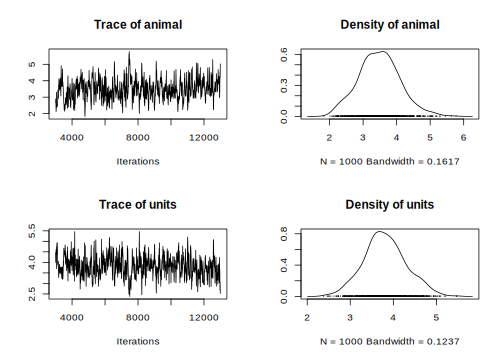
\includegraphics{wam_tuto_files/figure-latex/unnamed-chunk-33-1.pdf}
\caption{\label{fig:unnamed-chunk-33}The posterior distribution of the fixed effect (the intercept, or mean) in model 1.1}
\end{figure}

in the console, we get Figure 1 (p.~5). The plot on the left shows a time series of the values of 1000 samples of the posterior distribution of the the model intercept (mean birthweight). The plot on the right shows the same data as a distribution. Complicated statistical methods for estimating population means are of course of little interest; rather, we are examining these outputs to check that MCMCglmm's algorithms worked well for our data and for this model. The important point here is that a consistent amount of variation around a largely unchanging mean value of the intercept was obtained (which give this fluctuating trace concentrated around the mean), and the posterior distribution of the intercept appears to be valid. More rigorous means of evaluation the independence of the samples in the posterior distribution (evaluating autocorrelation) are discussed in the MCMCglmm CourseNotes, available from CRAN. Note that your output for \texttt{model\ 1.1} may not be identical to this due to Monte Carlo (random number) error. So every times, you run the model, you will get similar but slightly different results.

The posterior distributions of the the variance components are generally of more interest to animal model users. We can view plots of the posterior distribution for the variance components for model 1.1 by

\begin{Shaded}
\begin{Highlighting}[]
\KeywordTok{plot}\NormalTok{(model1}\FloatTok{.1}\OperatorTok{$}\NormalTok{VCV)}
\end{Highlighting}
\end{Shaded}

\begin{figure}
\centering
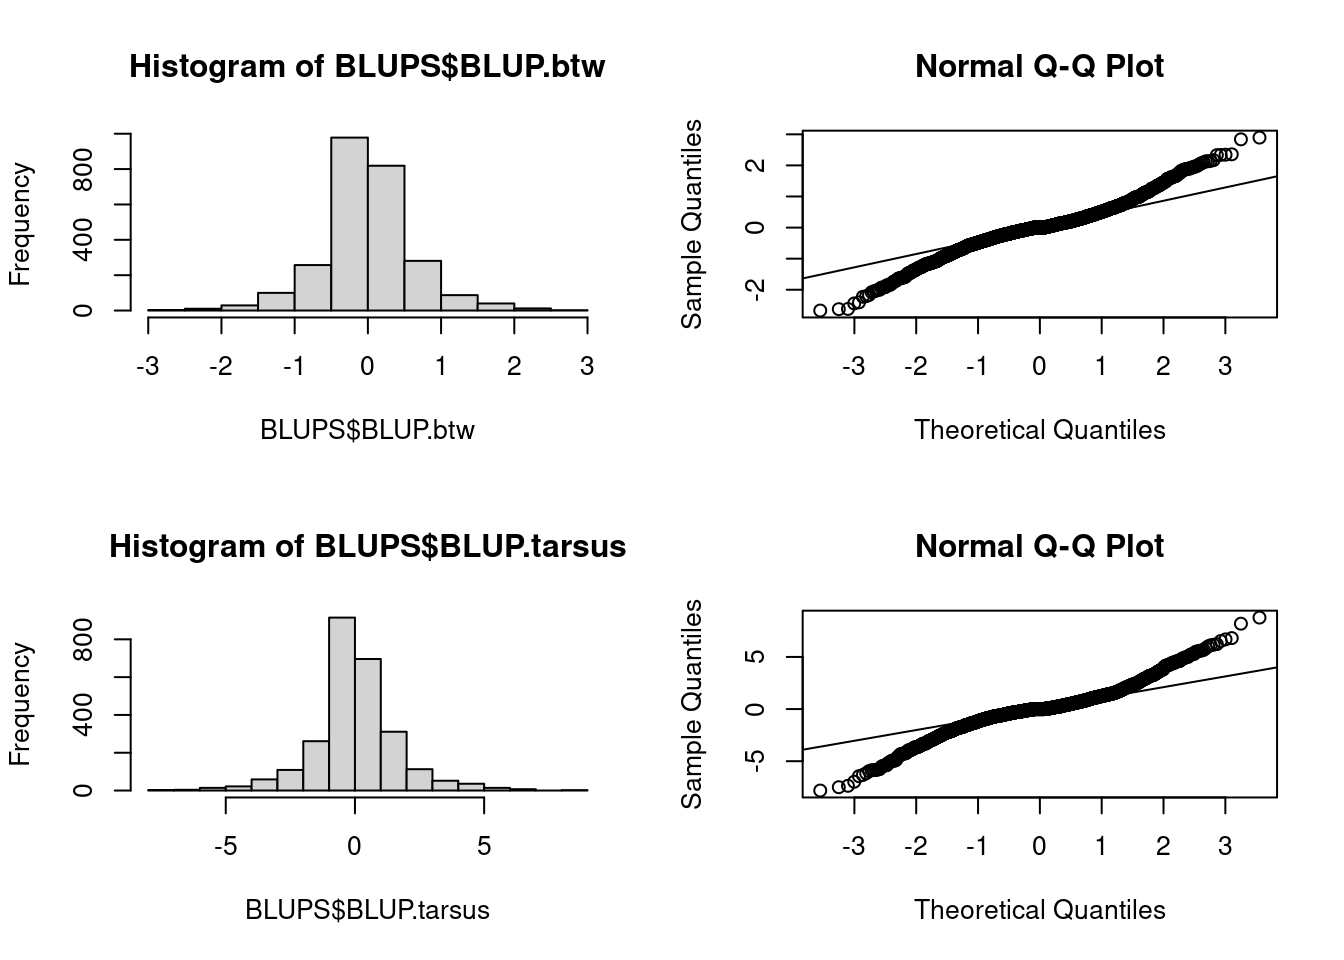
\includegraphics{wam_tuto_files/figure-latex/unnamed-chunk-34-1.pdf}
\caption{\label{fig:unnamed-chunk-34}The posterior distributions of the variance components of model 1.1, based on an analysis with the default values for nitt, burnin, and thin in MCMCglmm}
\end{figure}

which generates Figure 2 (p.~6). Here we see distributions of the estimates of the additive genetic (animal) and residual (units) effects. These samples contain some au- tocorrelation, i.e., trends are apparent in the left-hand plot. We can deal with this easily.

\hypertarget{change-in-iteration-and-sampling}{%
\subsection{Change in iteration and sampling}\label{change-in-iteration-and-sampling}}

We will simply re-run the model for a longer number of iterations, and sample the chain less frequently. So far we have been running MCMCglmm with its default values. These defaults are a total run length of 13000 iterations, the first 3000 of which are discarded as a `burn-in' period to make sure that the converges to the part of the parameter space where the maximum likelihood exists. The remaining 10000 iterations are sampled (estimates retained) every 10 iterations (the thinning interval). Because the values in the left-hand plots in figure 2 to appear to have different values at the beginning of the run, we might suspect that a longer burn-in period might be required. We can reduce the autocorrelation by lengthening the rest of the run and sampling the chain less frequently. The following code runs the same model 1.1, but is likely to produce better samples of the posterior distributions. This model should take about two minutes to analyze.

\begin{Shaded}
\begin{Highlighting}[]
\NormalTok{model1}\FloatTok{.1}\NormalTok{ \textless{}{-}}\StringTok{ }\KeywordTok{MCMCglmm}\NormalTok{(bwt }\OperatorTok{\textasciitilde{}}\StringTok{ }\DecValTok{1}\NormalTok{,}
  \DataTypeTok{random =} \OperatorTok{\textasciitilde{}}\NormalTok{animal, }\DataTypeTok{ginv =} \KeywordTok{list}\NormalTok{(}\DataTypeTok{animal =}\NormalTok{ Ainv),}
  \DataTypeTok{data =}\NormalTok{ gryphon, }\DataTypeTok{nitt =} \DecValTok{65000}\NormalTok{, }\DataTypeTok{thin =} \DecValTok{50}\NormalTok{, }\DataTypeTok{burnin =} \DecValTok{15000}\NormalTok{,}
  \DataTypeTok{prior =}\NormalTok{ prior1}\FloatTok{.1}\NormalTok{, }\DataTypeTok{verbose =} \OtherTok{FALSE}
\NormalTok{)}
\end{Highlighting}
\end{Shaded}

Notes that we have now included the argument verbose=FALSE in the MCMCglmm call. We will continue this throughout the tutorial so that more complete screen outputs can be included in this document without using too much space. Now produce the plots of the samples of the fixed and random effects (they have not been included in this document). Note that the autocorrelation is much reduced. A more compact way to evaluate the validity of the posterior distributions is to calculate autocorrelation among samples, as follows:

\begin{Shaded}
\begin{Highlighting}[]
\KeywordTok{autocorr.diag}\NormalTok{(model1}\FloatTok{.1}\OperatorTok{$}\NormalTok{VCV)}
\end{Highlighting}
\end{Shaded}

\begin{verbatim}
##                animal       units
## Lag 0     1.000000000  1.00000000
## Lag 50    0.161240748  0.10120248
## Lag 250   0.025673562 -0.02074865
## Lag 500  -0.005555388 -0.01507982
## Lag 2500  0.017485245  0.03811724
\end{verbatim}

We will consider these levels of autocorrelation acceptable, at least for the purposes of this tutorial. Ideally, all samples of the posterior distribution should be independent, and the autocorrelation for all lag values greater than zero should be near zero. However, in practice this will not strictly be achievable for all analytic scenarios. Certainly the levels of autocorrelation observed here should not be tolerated in any formal analysis.
Note that the validity of posterior distributions of any analysis should always be checked; however, for brevity we will not continue to be so consistently diligent throughout the rest of these tutorials. We can now proceed with confidence to recover some more information from these samples. We can obtain estimates of the additive genetic and residual variance by calculating the modes of the posterior distributions:

\begin{Shaded}
\begin{Highlighting}[]
\KeywordTok{posterior.mode}\NormalTok{(model1}\FloatTok{.1}\OperatorTok{$}\NormalTok{VCV)}
\end{Highlighting}
\end{Shaded}

\begin{verbatim}
##   animal    units 
## 3.390597 4.015234
\end{verbatim}

We can obtain the Bayesian equivalent of confidence intervals by calculating the the values of the estimates that bound 95\% (or any other proportion) of the posterior distributions:

\begin{Shaded}
\begin{Highlighting}[]
\KeywordTok{HPDinterval}\NormalTok{(model1}\FloatTok{.1}\OperatorTok{$}\NormalTok{VCV)}
\end{Highlighting}
\end{Shaded}

\begin{verbatim}
##           lower    upper
## animal 2.090187 4.586121
## units  2.854389 4.813375
## attr(,"Probability")
## [1] 0.95
\end{verbatim}

\hypertarget{change-priors-parameters}{%
\subsection{Change priors parameters}\label{change-priors-parameters}}

We specified weak priors in this analyses. Now we will check whether or not proper priors would have influenced the results that we obtained. The simplest way to do this is to rerun the model with different priors. In the previous model we specified a prior where the size of genetic and residual variance were similar. Here we construct priors with a larger degree of belief parameter (\texttt{nu}), and we will specify that a large proportion (95\%) of the variation is under genetic control (\texttt{V}):

\begin{Shaded}
\begin{Highlighting}[]
\NormalTok{p.var \textless{}{-}}\StringTok{ }\KeywordTok{var}\NormalTok{(gryphon}\OperatorTok{$}\NormalTok{bwt, }\DataTypeTok{na.rm =} \OtherTok{TRUE}\NormalTok{)}
\NormalTok{prior1.}\FloatTok{1.2}\NormalTok{ \textless{}{-}}\StringTok{ }\KeywordTok{list}\NormalTok{(}
  \DataTypeTok{G =} \KeywordTok{list}\NormalTok{(}\DataTypeTok{G1 =} \KeywordTok{list}\NormalTok{(}\DataTypeTok{V =} \KeywordTok{matrix}\NormalTok{(p.var }\OperatorTok{*}\StringTok{ }\FloatTok{0.95}\NormalTok{), }\DataTypeTok{nu =} \DecValTok{1}\NormalTok{)),}
  \DataTypeTok{R =} \KeywordTok{list}\NormalTok{(}\DataTypeTok{V =} \KeywordTok{matrix}\NormalTok{(p.var }\OperatorTok{*}\StringTok{ }\FloatTok{0.05}\NormalTok{), }\DataTypeTok{nu =} \DecValTok{1}\NormalTok{)}
\NormalTok{)}

\NormalTok{model1.}\FloatTok{1.2}\NormalTok{ \textless{}{-}}\StringTok{ }\KeywordTok{MCMCglmm}\NormalTok{(bwt }\OperatorTok{\textasciitilde{}}\StringTok{ }\DecValTok{1}\NormalTok{,}
  \DataTypeTok{random =} \OperatorTok{\textasciitilde{}}\NormalTok{animal, }\DataTypeTok{ginv =} \KeywordTok{list}\NormalTok{(}\DataTypeTok{animal =}\NormalTok{ Ainv),}
  \DataTypeTok{data =}\NormalTok{ gryphon, }\DataTypeTok{prior =}\NormalTok{ prior1.}\FloatTok{1.2}\NormalTok{, }\DataTypeTok{nitt =} \DecValTok{65000}\NormalTok{, }\DataTypeTok{thin =} \DecValTok{50}\NormalTok{,}
  \DataTypeTok{burnin =} \DecValTok{15000}\NormalTok{, }\DataTypeTok{verbose =} \OtherTok{FALSE}
\NormalTok{)}
\KeywordTok{posterior.mode}\NormalTok{(model1}\FloatTok{.1}\OperatorTok{$}\NormalTok{VCV)}
\end{Highlighting}
\end{Shaded}

\begin{verbatim}
##   animal    units 
## 3.390597 4.015234
\end{verbatim}

\begin{Shaded}
\begin{Highlighting}[]
\KeywordTok{posterior.mode}\NormalTok{(model1.}\FloatTok{1.2}\OperatorTok{$}\NormalTok{VCV)}
\end{Highlighting}
\end{Shaded}

\begin{verbatim}
##   animal    units 
## 3.198105 3.647427
\end{verbatim}

and we can therefore conclude that the difference in the priors has little effect on the outcome of the analysis. This is typical for an analysis where lots of data are available relative to the complexity of the model, but is often not the case. In all cases, it is important to check the effect of priors on conclusions drawn from a model. In addition, you can also specify the prior with previous knowledge or expectation for the variance.

\hypertarget{estimating-heritability-1}{%
\subsection{Estimating heritability}\label{estimating-heritability-1}}

A useful property of Bayesian posterior distributions is that we can apply almost any transformation to these distributions and they will remain valid. This applies to the calculation of heritabilities. We can obtain an estimate of the heritability by applying the basic formula \(h^2\) =\(V_A /V_P\) to each sample of the posterior disribution:

\begin{Shaded}
\begin{Highlighting}[]
\NormalTok{posterior.heritability1}\FloatTok{.1}\NormalTok{ \textless{}{-}}\StringTok{ }\NormalTok{model1}\FloatTok{.1}\OperatorTok{$}\NormalTok{VCV[, }\StringTok{"animal"}\NormalTok{] }\OperatorTok{/}\StringTok{ }
\StringTok{  }\NormalTok{(model1}\FloatTok{.1}\OperatorTok{$}\NormalTok{VCV[, }\StringTok{"animal"}\NormalTok{] }\OperatorTok{+}\StringTok{ }\NormalTok{model1}\FloatTok{.1}\OperatorTok{$}\NormalTok{VCV[, }\StringTok{"units"}\NormalTok{])}
\KeywordTok{HPDinterval}\NormalTok{(posterior.heritability1}\FloatTok{.1}\NormalTok{, }\FloatTok{0.95}\NormalTok{)}
\end{Highlighting}
\end{Shaded}

\begin{verbatim}
##          lower     upper
## var1 0.3231535 0.6174858
## attr(,"Probability")
## [1] 0.95
\end{verbatim}

\begin{Shaded}
\begin{Highlighting}[]
\KeywordTok{posterior.mode}\NormalTok{(posterior.heritability1}\FloatTok{.1}\NormalTok{)}
\end{Highlighting}
\end{Shaded}

\begin{verbatim}
##      var1 
## 0.4860597
\end{verbatim}

Generate a plot of the posterior distribution of this heritability estimate:

\begin{Shaded}
\begin{Highlighting}[]
\KeywordTok{plot}\NormalTok{(posterior.heritability1}\FloatTok{.1}\NormalTok{)}
\end{Highlighting}
\end{Shaded}

\begin{figure}
\centering
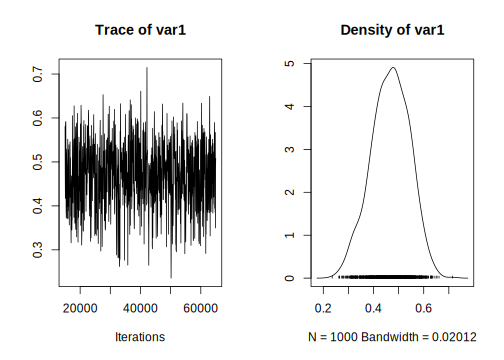
\includegraphics{wam_tuto_files/figure-latex/unnamed-chunk-41-1.pdf}
\caption{\label{fig:unnamed-chunk-41}The posterior distributions the heritability from model 1.1}
\end{figure}

\hypertarget{adding-fixed-effects-1}{%
\subsection{Adding fixed effects}\label{adding-fixed-effects-1}}

To add effects to a univariate model, we simply modify the fixed effect part of the model specification:

\begin{Shaded}
\begin{Highlighting}[]
\NormalTok{model1}\FloatTok{.2}\NormalTok{ \textless{}{-}}\StringTok{ }\KeywordTok{MCMCglmm}\NormalTok{(bwt }\OperatorTok{\textasciitilde{}}\StringTok{ }\NormalTok{sex,}
  \DataTypeTok{random =} \OperatorTok{\textasciitilde{}}\NormalTok{animal, }\DataTypeTok{ginv =} \KeywordTok{list}\NormalTok{(}\DataTypeTok{animal =}\NormalTok{ Ainv),}
  \DataTypeTok{data =}\NormalTok{ gryphon, }\DataTypeTok{prior =}\NormalTok{ prior1}\FloatTok{.1}\NormalTok{,}
  \DataTypeTok{nitt =} \DecValTok{65000}\NormalTok{, }\DataTypeTok{thin =} \DecValTok{50}\NormalTok{, }\DataTypeTok{burnin =} \DecValTok{15000}\NormalTok{, }\DataTypeTok{verbose =} \OtherTok{FALSE}
\NormalTok{)}
\end{Highlighting}
\end{Shaded}

We can assess the significance of \texttt{sex} as a fixed effect by examining its posterior distribution.

\begin{Shaded}
\begin{Highlighting}[]
\KeywordTok{posterior.mode}\NormalTok{(model1}\FloatTok{.2}\OperatorTok{$}\NormalTok{Sol[, }\StringTok{"sex2"}\NormalTok{])}
\end{Highlighting}
\end{Shaded}

\begin{verbatim}
##     var1 
## 2.177682
\end{verbatim}

\begin{Shaded}
\begin{Highlighting}[]
\KeywordTok{HPDinterval}\NormalTok{(model1}\FloatTok{.2}\OperatorTok{$}\NormalTok{Sol[, }\StringTok{"sex2"}\NormalTok{], }\FloatTok{0.95}\NormalTok{)}
\end{Highlighting}
\end{Shaded}

\begin{verbatim}
##         lower    upper
## var1 1.899605 2.516297
## attr(,"Probability")
## [1] 0.95
\end{verbatim}

The posterior distribution of the \texttt{sex2} term does not overlap zero. Thus, we can infer that sex has an effect on birthweight (presence of a sexual dimorphism) in this model and is a useful addition to the model, for most purposes. It is also worth noting that the variance components have changed slightly:

\begin{Shaded}
\begin{Highlighting}[]
\KeywordTok{posterior.mode}\NormalTok{(model1}\FloatTok{.2}\OperatorTok{$}\NormalTok{VCV)}
\end{Highlighting}
\end{Shaded}

\begin{verbatim}
##   animal    units 
## 3.186636 3.128075
\end{verbatim}

In fact since sex effects were previously contributing to the residual variance of the model our estimate of \(V_R\) (denoted 'units' in the output) is now slightly lower than before. This has an important consequence for estimating heritability since if we calculate \(V_P\) as \(V_A +V_R\) then as we include fixed effects we will soak up more residual variance driving \(V_P\) . Assuming that \(V_A\) is more or less unaffected by the fixed effects fitted then as \(V_P\) goes down we expect our estimate of \(h^2\) will go up.

\begin{Shaded}
\begin{Highlighting}[]
\NormalTok{posterior.heritability1}\FloatTok{.2}\NormalTok{ \textless{}{-}}\StringTok{ }\NormalTok{model1}\FloatTok{.2}\OperatorTok{$}\NormalTok{VCV[, }\StringTok{"animal"}\NormalTok{] }\OperatorTok{/}
\StringTok{  }\NormalTok{(model1}\FloatTok{.2}\OperatorTok{$}\NormalTok{VCV[, }\StringTok{"animal"}\NormalTok{] }\OperatorTok{+}\StringTok{ }\NormalTok{model1}\FloatTok{.2}\OperatorTok{$}\NormalTok{VCV[, }\StringTok{"units"}\NormalTok{])}
\KeywordTok{posterior.mode}\NormalTok{(posterior.heritability1}\FloatTok{.2}\NormalTok{)}
\end{Highlighting}
\end{Shaded}

\begin{verbatim}
##      var1 
## 0.5163052
\end{verbatim}

\begin{Shaded}
\begin{Highlighting}[]
\KeywordTok{HPDinterval}\NormalTok{(posterior.heritability1}\FloatTok{.2}\NormalTok{, }\FloatTok{0.95}\NormalTok{)}
\end{Highlighting}
\end{Shaded}

\begin{verbatim}
##          lower     upper
## var1 0.3654759 0.6321316
## attr(,"Probability")
## [1] 0.95
\end{verbatim}

Here \(h^2\) has increased slightly from 0.4829 to 0.5079 (again, your values may differ slightly due to Monte Carlo error). Which is the better estimate?
It depends on what your question is. The first is an estimate of the proportion of variance in birth weight explained by additive effects, the latter is an estimate of the proportion of variance in birth weight after conditioning on sex that is explained by additive effects.
An important piece of advice, each researcher should be consistent in how they name their estimates and always correctly describe which estimates they are using conditional or not (to avoid any confusion).

\hypertarget{adding-random-effects-1}{%
\subsection{Adding random effects}\label{adding-random-effects-1}}

This is done by simply modifying the model statement in the same way, but requires addition of a prior for the new random effect. For instance, we can fit an effect of birth year:

\begin{Shaded}
\begin{Highlighting}[]
\NormalTok{prior1}\FloatTok{.3}\NormalTok{ \textless{}{-}}\StringTok{ }\KeywordTok{list}\NormalTok{(}
  \DataTypeTok{G =} \KeywordTok{list}\NormalTok{(}\DataTypeTok{G1 =} \KeywordTok{list}\NormalTok{(}\DataTypeTok{V =} \DecValTok{1}\NormalTok{, }\DataTypeTok{nu =} \FloatTok{0.002}\NormalTok{), }\DataTypeTok{G2 =} \KeywordTok{list}\NormalTok{(}\DataTypeTok{V =} \DecValTok{1}\NormalTok{, }\DataTypeTok{nu =} \FloatTok{0.002}\NormalTok{)),}
  \DataTypeTok{R =} \KeywordTok{list}\NormalTok{(}\DataTypeTok{V =} \DecValTok{1}\NormalTok{, }\DataTypeTok{nu =} \FloatTok{0.002}\NormalTok{))}
\NormalTok{model1}\FloatTok{.3}\NormalTok{ \textless{}{-}}\StringTok{ }\KeywordTok{MCMCglmm}\NormalTok{(bwt }\OperatorTok{\textasciitilde{}}\StringTok{ }\NormalTok{sex,}
  \DataTypeTok{random =} \OperatorTok{\textasciitilde{}}\StringTok{ }\NormalTok{animal }\OperatorTok{+}\StringTok{ }\NormalTok{byear, }\DataTypeTok{ginv =} \KeywordTok{list}\NormalTok{(}\DataTypeTok{animal =}\NormalTok{ Ainv),}
  \DataTypeTok{data =}\NormalTok{ gryphon,}
  \DataTypeTok{nitt =} \DecValTok{65000}\NormalTok{, }\DataTypeTok{thin =} \DecValTok{50}\NormalTok{, }\DataTypeTok{burnin =} \DecValTok{15000}\NormalTok{,}
  \DataTypeTok{prior =}\NormalTok{ prior1}\FloatTok{.3}\NormalTok{, }\DataTypeTok{verbose =} \OtherTok{FALSE}
\NormalTok{)}
\KeywordTok{posterior.mode}\NormalTok{(model1}\FloatTok{.3}\OperatorTok{$}\NormalTok{VCV)}
\end{Highlighting}
\end{Shaded}

\begin{verbatim}
##    animal     byear     units 
## 2.7126159 0.8999305 2.1446505
\end{verbatim}

Here the variance in birth weight explained by birth year is 0.7887. Note that although \(V_A\) has changed somewhat, most of what is now partitioned as a \texttt{birth\ year} effect was previously partitioned as \(V_R\) . Thus what we have really done here is to partition environmental effects into those arising from year to year differences versus everything else, and we do not really expect much change in \(h^2\) (since now \(h^2 = V_A /(V_A + V_{BY} + V_R )\)). However, we get a somewhat different result if we also add a random effect of \texttt{mother} to test for maternal effects:

\begin{Shaded}
\begin{Highlighting}[]
\NormalTok{p.var \textless{}{-}}\StringTok{ }\KeywordTok{var}\NormalTok{(gryphon}\OperatorTok{$}\NormalTok{bwt, }\DataTypeTok{na.rm =} \OtherTok{TRUE}\NormalTok{)}
\NormalTok{prior1}\FloatTok{.4}\NormalTok{ \textless{}{-}}\StringTok{ }\KeywordTok{list}\NormalTok{(}
  \DataTypeTok{G =} \KeywordTok{list}\NormalTok{(}
    \DataTypeTok{G1 =} \KeywordTok{list}\NormalTok{(}\DataTypeTok{V =} \DecValTok{1}\NormalTok{, }\DataTypeTok{nu =} \FloatTok{0.002}\NormalTok{),}
    \DataTypeTok{G2 =} \KeywordTok{list}\NormalTok{(}\DataTypeTok{V =} \DecValTok{1}\NormalTok{, }\DataTypeTok{nu =} \FloatTok{0.002}\NormalTok{),}
    \DataTypeTok{G3 =} \KeywordTok{list}\NormalTok{(}\DataTypeTok{V =} \DecValTok{1}\NormalTok{, }\DataTypeTok{nu =} \FloatTok{0.002}\NormalTok{)),}
  \DataTypeTok{R =} \KeywordTok{list}\NormalTok{(}\DataTypeTok{V =} \DecValTok{1}\NormalTok{, }\DataTypeTok{nu =} \FloatTok{0.002}\NormalTok{)}
\NormalTok{)}
\NormalTok{model1}\FloatTok{.4}\NormalTok{ \textless{}{-}}\StringTok{ }\KeywordTok{MCMCglmm}\NormalTok{(bwt }\OperatorTok{\textasciitilde{}}\StringTok{ }\NormalTok{sex,}
  \DataTypeTok{random =} \OperatorTok{\textasciitilde{}}\StringTok{ }\NormalTok{animal }\OperatorTok{+}\StringTok{ }\NormalTok{byear }\OperatorTok{+}\StringTok{ }\NormalTok{mother,}
  \DataTypeTok{ginv =} \KeywordTok{list}\NormalTok{(}\DataTypeTok{animal =}\NormalTok{ Ainv), }\DataTypeTok{data =}\NormalTok{ gryphon,}
  \DataTypeTok{nitt =} \DecValTok{65000}\NormalTok{, }\DataTypeTok{thin =} \DecValTok{50}\NormalTok{, }\DataTypeTok{burnin =} \DecValTok{15000}\NormalTok{,}
  \DataTypeTok{prior =}\NormalTok{ prior1}\FloatTok{.4}\NormalTok{, }\DataTypeTok{verbose =} \OtherTok{FALSE}
\NormalTok{)}
\KeywordTok{posterior.mode}\NormalTok{(model1}\FloatTok{.4}\OperatorTok{$}\NormalTok{VCV)}
\end{Highlighting}
\end{Shaded}

\begin{verbatim}
##    animal     byear    mother     units 
## 2.2735066 0.8767165 1.2756643 1.7195274
\end{verbatim}

Here partitioning of significant maternal variance has resulted in a further decrease in \(V_R\) but also a decrease in \(V_A\). The latter is because maternal effects of the sort we simulated (fixed differences between mothers) will have the consequence of increasing similarity among maternal siblings. Consequently they can look very much like additive genetic effects and if present, but unmodelled, represent a type of `common environment effect' that can - and will- cause upward bias in \(V_A\) and so \(h^2\). Let's compare the estimates of heritability from each of models 1.2, 1.3 and 1.4:

\begin{Shaded}
\begin{Highlighting}[]
\NormalTok{posterior.heritability1}\FloatTok{.3}\NormalTok{ \textless{}{-}}\StringTok{ }\NormalTok{model1}\FloatTok{.3}\OperatorTok{$}\NormalTok{VCV[, }\StringTok{"animal"}\NormalTok{] }\OperatorTok{/}
\StringTok{  }\NormalTok{(model1}\FloatTok{.3}\OperatorTok{$}\NormalTok{VCV[, }\StringTok{"animal"}\NormalTok{] }\OperatorTok{+}\StringTok{ }\NormalTok{model1}\FloatTok{.3}\OperatorTok{$}\NormalTok{VCV[, }\StringTok{"byear"}\NormalTok{] }\OperatorTok{+}\StringTok{ }\NormalTok{model1}\FloatTok{.3}\OperatorTok{$}\NormalTok{VCV[, }\StringTok{"units"}\NormalTok{])}
\NormalTok{posterior.heritability1}\FloatTok{.4}\NormalTok{ \textless{}{-}}\StringTok{ }\NormalTok{model1}\FloatTok{.4}\OperatorTok{$}\NormalTok{VCV[, }\StringTok{"animal"}\NormalTok{] }\OperatorTok{/}
\StringTok{  }\NormalTok{(model1}\FloatTok{.4}\OperatorTok{$}\NormalTok{VCV[, }\StringTok{"animal"}\NormalTok{] }\OperatorTok{+}\StringTok{ }\NormalTok{model1}\FloatTok{.4}\OperatorTok{$}\NormalTok{VCV[, }\StringTok{"byear"}\NormalTok{] }\OperatorTok{+}\StringTok{ }\NormalTok{model1}\FloatTok{.4}\OperatorTok{$}\NormalTok{VCV[, }\StringTok{"mother"}\NormalTok{] }\OperatorTok{+}\StringTok{ }\NormalTok{model1}\FloatTok{.4}\OperatorTok{$}\NormalTok{VCV[, }\StringTok{"units"}\NormalTok{])}
\KeywordTok{posterior.mode}\NormalTok{(posterior.heritability1}\FloatTok{.2}\NormalTok{)}
\end{Highlighting}
\end{Shaded}

\begin{verbatim}
##      var1 
## 0.5163052
\end{verbatim}

\begin{Shaded}
\begin{Highlighting}[]
\KeywordTok{posterior.mode}\NormalTok{(posterior.heritability1}\FloatTok{.3}\NormalTok{)}
\end{Highlighting}
\end{Shaded}

\begin{verbatim}
##      var1 
## 0.4366087
\end{verbatim}

\begin{Shaded}
\begin{Highlighting}[]
\KeywordTok{posterior.mode}\NormalTok{(posterior.heritability1}\FloatTok{.4}\NormalTok{)}
\end{Highlighting}
\end{Shaded}

\begin{verbatim}
##      var1 
## 0.3954481
\end{verbatim}

\hypertarget{testing-significance-of-variance-components}{%
\subsection{Testing significance of variance components}\label{testing-significance-of-variance-components}}

While testing the significance of fixed effects by evaluating whether or not their posterior distributions overlap zero was simple and valid, this approach does not work for variance components.
Variance components are bounded to be positive (given a proper prior), and thus even when a random effect is not meaningful, its posterior distribution will never overlap zero. Model comparisons can be performed using the deviance information criterion (\texttt{DIC}), although it should be noted that the properties of DIC are not well understood and that the \texttt{DIC} may be focused at the wrong level for most people's intended level of inference - particularly with non-Gaussian responses. The implementation of \texttt{DIC} in MCMCglmm is further described in the reference manual. \texttt{DIC} values are calculated by MCMCglmm by default. Briefly, \texttt{DIC} like other information criteria balance model fit and model complexity simultaneously, and small values of DIC are preferred. We can compare \texttt{models\ 1.4} and \texttt{1.3}, i.e., models with and without the mother term:

\begin{Shaded}
\begin{Highlighting}[]
\NormalTok{model1}\FloatTok{.3}\OperatorTok{$}\NormalTok{DIC}
\end{Highlighting}
\end{Shaded}

\begin{verbatim}
## [1] 3551.509
\end{verbatim}

\begin{Shaded}
\begin{Highlighting}[]
\NormalTok{model1}\FloatTok{.4}\OperatorTok{$}\NormalTok{DIC}
\end{Highlighting}
\end{Shaded}

\begin{verbatim}
## [1] 3294.081
\end{verbatim}

\texttt{model\ 1.4} has a much lower DIC value. Since the maternal effect term is the only difference between the models, we can consider the inclusion of this term statistically justifiable. We should note however that DIC has a large sampling variance and should probably only be calculated based on much longer MCMC runs.

\hypertarget{further-partitioning-variance}{%
\subsection{Further partitioning variance}\label{further-partitioning-variance}}

A population can be further fragmented into different groups or categories (such as females and males, juveniles and adults or treated and untreated). Some scientific questions require further and deeper analysis of the variance.
To avoid multiple model (one for each group), we can directly partition the variance between groups in a unique model. In addition, by doing so, we can also test if the variance are different between groups.

As example, we can partition the additive genetic variance and residual variance by sex. It is impossible to further partition the other variances but complexify an animal model requires sufficient sample size.

\begin{Shaded}
\begin{Highlighting}[]
\NormalTok{prior1.}\FloatTok{4.}\NormalTok{SEX \textless{}{-}}\StringTok{ }\KeywordTok{list}\NormalTok{(}
  \DataTypeTok{G =} \KeywordTok{list}\NormalTok{(}\DataTypeTok{G1 =} \KeywordTok{list}\NormalTok{(}\DataTypeTok{V =} \KeywordTok{diag}\NormalTok{(}\DecValTok{2}\NormalTok{), }\DataTypeTok{nu =} \FloatTok{1.002}\NormalTok{), }\DataTypeTok{G2 =} \KeywordTok{list}\NormalTok{(}\DataTypeTok{V =} \DecValTok{1}\NormalTok{, }\DataTypeTok{nu =} \FloatTok{0.002}\NormalTok{), }\DataTypeTok{G3 =} \KeywordTok{list}\NormalTok{(}\DataTypeTok{V =} \DecValTok{1}\NormalTok{, }\DataTypeTok{nu =} \FloatTok{0.002}\NormalTok{)),}
  \DataTypeTok{R =} \KeywordTok{list}\NormalTok{(}\DataTypeTok{V =} \KeywordTok{diag}\NormalTok{(}\DecValTok{2}\NormalTok{), }\DataTypeTok{nu =} \FloatTok{1.002}\NormalTok{)}
\NormalTok{)}

\NormalTok{model1.}\FloatTok{4.}\NormalTok{SEX \textless{}{-}}\StringTok{ }\KeywordTok{MCMCglmm}\NormalTok{(bwt }\OperatorTok{\textasciitilde{}}\StringTok{ }\NormalTok{sex,}
  \DataTypeTok{random =} \OperatorTok{\textasciitilde{}}\StringTok{ }\KeywordTok{idh}\NormalTok{(sex)}\OperatorTok{:}\NormalTok{animal }\OperatorTok{+}\StringTok{ }\NormalTok{byear }\OperatorTok{+}\StringTok{ }\NormalTok{mother,}
  \DataTypeTok{rcov =} \OperatorTok{\textasciitilde{}}\StringTok{ }\KeywordTok{idh}\NormalTok{(sex)}\OperatorTok{:}\NormalTok{units,}
  \DataTypeTok{ginv =} \KeywordTok{list}\NormalTok{(}\DataTypeTok{animal =}\NormalTok{ Ainv), }\DataTypeTok{data =}\NormalTok{ gryphon, }\DataTypeTok{nitt =} \DecValTok{65000}\NormalTok{, }\DataTypeTok{thin =} \DecValTok{50}\NormalTok{, }\DataTypeTok{burnin =} \DecValTok{15000}\NormalTok{,}
  \DataTypeTok{prior =}\NormalTok{ prior1.}\FloatTok{4.}\NormalTok{SEX, }\DataTypeTok{verbose =} \OtherTok{FALSE}
\NormalTok{)}
\KeywordTok{posterior.mode}\NormalTok{(model1.}\FloatTok{4.}\NormalTok{SEX}\OperatorTok{$}\NormalTok{VCV)}
\end{Highlighting}
\end{Shaded}

\begin{verbatim}
## sex1.animal sex2.animal       byear      mother  sex1.units  sex2.units 
##   1.3483958   1.5118838   0.9123085   1.2122629   2.0206409   1.5236338
\end{verbatim}

\begin{Shaded}
\begin{Highlighting}[]
\NormalTok{posterior.heritability1.}\FloatTok{4.}\NormalTok{FEM \textless{}{-}}\StringTok{ }\NormalTok{model1.}\FloatTok{4.}\NormalTok{SEX}\OperatorTok{$}\NormalTok{VCV[, }\StringTok{"sex1.animal"}\NormalTok{] }\OperatorTok{/}
\StringTok{  }\NormalTok{(model1.}\FloatTok{4.}\NormalTok{SEX}\OperatorTok{$}\NormalTok{VCV[, }\StringTok{"sex1.animal"}\NormalTok{] }\OperatorTok{+}\StringTok{ }\NormalTok{model1.}\FloatTok{4.}\NormalTok{SEX}\OperatorTok{$}\NormalTok{VCV[, }\StringTok{"byear"}\NormalTok{] }\OperatorTok{+}
\StringTok{   }\NormalTok{model1.}\FloatTok{4.}\NormalTok{SEX}\OperatorTok{$}\NormalTok{VCV[, }\StringTok{"mother"}\NormalTok{] }\OperatorTok{+}\StringTok{ }\NormalTok{model1.}\FloatTok{4.}\NormalTok{SEX}\OperatorTok{$}\NormalTok{VCV[, }\StringTok{"sex1.units"}\NormalTok{])}
\NormalTok{posterior.heritability1.}\FloatTok{4.}\NormalTok{MAL \textless{}{-}}\StringTok{ }\NormalTok{model1.}\FloatTok{4.}\NormalTok{SEX}\OperatorTok{$}\NormalTok{VCV[, }\StringTok{"sex2.animal"}\NormalTok{] }\OperatorTok{/}
\StringTok{  }\NormalTok{(model1.}\FloatTok{4.}\NormalTok{SEX}\OperatorTok{$}\NormalTok{VCV[, }\StringTok{"sex2.animal"}\NormalTok{] }\OperatorTok{+}\StringTok{ }\NormalTok{model1.}\FloatTok{4.}\NormalTok{SEX}\OperatorTok{$}\NormalTok{VCV[, }\StringTok{"byear"}\NormalTok{] }\OperatorTok{+}
\StringTok{   }\NormalTok{model1.}\FloatTok{4.}\NormalTok{SEX}\OperatorTok{$}\NormalTok{VCV[, }\StringTok{"mother"}\NormalTok{] }\OperatorTok{+}\StringTok{ }\NormalTok{model1.}\FloatTok{4.}\NormalTok{SEX}\OperatorTok{$}\NormalTok{VCV[, }\StringTok{"sex2.units"}\NormalTok{])}

\KeywordTok{posterior.mode}\NormalTok{(posterior.heritability1.}\FloatTok{4.}\NormalTok{FEM)}
\end{Highlighting}
\end{Shaded}

\begin{verbatim}
##      var1 
## 0.2048813
\end{verbatim}

\begin{Shaded}
\begin{Highlighting}[]
\KeywordTok{HPDinterval}\NormalTok{(posterior.heritability1.}\FloatTok{4.}\NormalTok{FEM, }\FloatTok{0.95}\NormalTok{)}
\end{Highlighting}
\end{Shaded}

\begin{verbatim}
##           lower     upper
## var1 0.04604999 0.4421084
## attr(,"Probability")
## [1] 0.95
\end{verbatim}

\begin{Shaded}
\begin{Highlighting}[]
\KeywordTok{posterior.mode}\NormalTok{(posterior.heritability1.}\FloatTok{4.}\NormalTok{MAL)}
\end{Highlighting}
\end{Shaded}

\begin{verbatim}
##      var1 
## 0.4239716
\end{verbatim}

\begin{Shaded}
\begin{Highlighting}[]
\KeywordTok{HPDinterval}\NormalTok{(posterior.heritability1.}\FloatTok{4.}\NormalTok{MAL, }\FloatTok{0.95}\NormalTok{)}
\end{Highlighting}
\end{Shaded}

\begin{verbatim}
##           lower    upper
## var1 0.05701948 0.595573
## attr(,"Probability")
## [1] 0.95
\end{verbatim}

Here, we can estimate the heritability for each sex. Both doesn't overlap with zero, so we can conclude both sexes have significant heritability. However due to their overlaps CIs, we can not conclude the heritability is not significantly different between sexes.
An important quote to remember is ``A difference in significance is not a significant difference''

\hypertarget{modification-of-model-parameter-1}{%
\subsection{\texorpdfstring{Modification of model parameter }{Modification of model parameter }}\label{modification-of-model-parameter-1}}

\hypertarget{covariance-between-two-random-effects-1}{%
\subsection{Covariance between two random effects}\label{covariance-between-two-random-effects-1}}

\hypertarget{brms-1}{%
\section{brms}\label{brms-1}}

\hypertarget{running-the-model-2}{%
\subsection{Running the model}\label{running-the-model-2}}

First we need to load the \texttt{brms} library:

\begin{Shaded}
\begin{Highlighting}[]
\KeywordTok{library}\NormalTok{(brms)}
\end{Highlighting}
\end{Shaded}

\begin{verbatim}
## Loading required package: Rcpp
\end{verbatim}

\begin{verbatim}
## Loading 'brms' package (version 2.16.1). Useful instructions
## can be found by typing help('brms'). A more detailed introduction
## to the package is available through vignette('brms_overview').
\end{verbatim}

\begin{verbatim}
## 
## Attaching package: 'brms'
\end{verbatim}

\begin{verbatim}
## The following object is masked from 'package:MCMCglmm':
## 
##     me
\end{verbatim}

\begin{verbatim}
## The following object is masked from 'package:stats':
## 
##     ar
\end{verbatim}

To be able to fit an animal model, brms needs the relationship matrix (and not its inverse as in other softwares).
This can be estimated using the \texttt{nadiv} package

\begin{Shaded}
\begin{Highlighting}[]
\NormalTok{Amat \textless{}{-}}\StringTok{ }\KeywordTok{as.matrix}\NormalTok{(nadiv}\OperatorTok{::}\KeywordTok{makeA}\NormalTok{(gryphonped))}
\end{Highlighting}
\end{Shaded}

We are now ready to specify our first model:
The structure of a bmrs model is similar to \texttt{lme4}, the random effect is added to the model with the term \texttt{(1\ \textbar{}\ gr(animal,\ cov\ =\ Amat)}. ()

\begin{Shaded}
\begin{Highlighting}[]
\NormalTok{brms\_m1}\FloatTok{.1}\NormalTok{ \textless{}{-}}\StringTok{ }\KeywordTok{brm}\NormalTok{(}
\NormalTok{  bwt }\OperatorTok{\textasciitilde{}}\StringTok{ }\DecValTok{1} \OperatorTok{+}\StringTok{ }\NormalTok{(}\DecValTok{1} \OperatorTok{|}\StringTok{ }\KeywordTok{gr}\NormalTok{(animal, }\DataTypeTok{cov =}\NormalTok{ Amat)),}
  \DataTypeTok{data =}\NormalTok{ gryphon,}
  \DataTypeTok{data2 =} \KeywordTok{list}\NormalTok{(}\DataTypeTok{Amat =}\NormalTok{ Amat),}
  \DataTypeTok{family =} \KeywordTok{gaussian}\NormalTok{(),}
  \DataTypeTok{chains =} \DecValTok{2}\NormalTok{, }\DataTypeTok{cores =} \DecValTok{2}\NormalTok{, }\DataTypeTok{iter =} \DecValTok{1000}
\NormalTok{)}
\KeywordTok{save}\NormalTok{(brms\_m1}\FloatTok{.1}\NormalTok{, }\DataTypeTok{file =} \StringTok{"data/brms\_m1\_1.rda"}\NormalTok{)}
\end{Highlighting}
\end{Shaded}

The result of the long model calculation is save in a spare file \texttt{brms\_m1\_1.rda"}.
reloading it, we can examine (or directly using the model) the variance estimate and their distributions
It is also possible to calcule the heritability using xxx

\begin{Shaded}
\begin{Highlighting}[]
\KeywordTok{load}\NormalTok{(}\StringTok{"data/brms\_m1\_1.rda"}\NormalTok{)}
\KeywordTok{summary}\NormalTok{(brms\_m1}\FloatTok{.1}\NormalTok{)}
\end{Highlighting}
\end{Shaded}

\begin{verbatim}
##  Family: gaussian 
##   Links: mu = identity; sigma = identity 
## Formula: bwt ~ 1 + (1 | gr(animal, cov = Amat)) 
##    Data: gryphon (Number of observations: 854) 
##   Draws: 2 chains, each with iter = 1000; warmup = 500; thin = 1;
##          total post-warmup draws = 1000
## 
## Group-Level Effects: 
## ~animal (Number of levels: 854) 
##               Estimate Est.Error l-95% CI u-95% CI Rhat Bulk_ESS Tail_ESS
## sd(Intercept)     1.88      0.17     1.54     2.23 1.03       74       99
## 
## Population-Level Effects: 
##           Estimate Est.Error l-95% CI u-95% CI Rhat Bulk_ESS Tail_ESS
## Intercept     7.60      0.14     7.33     7.86 1.01      428      727
## 
## Family Specific Parameters: 
##       Estimate Est.Error l-95% CI u-95% CI Rhat Bulk_ESS Tail_ESS
## sigma     1.93      0.13     1.66     2.18 1.04       71      112
## 
## Draws were sampled using sampling(NUTS). For each parameter, Bulk_ESS
## and Tail_ESS are effective sample size measures, and Rhat is the potential
## scale reduction factor on split chains (at convergence, Rhat = 1).
\end{verbatim}

\begin{Shaded}
\begin{Highlighting}[]
\KeywordTok{plot}\NormalTok{(brms\_m1}\FloatTok{.1}\NormalTok{)}
\end{Highlighting}
\end{Shaded}

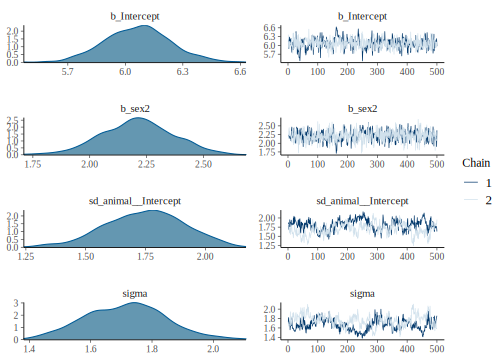
\includegraphics{wam_tuto_files/figure-latex/unnamed-chunk-54-1.pdf}

\begin{Shaded}
\begin{Highlighting}[]
\NormalTok{v\_animal \textless{}{-}}\StringTok{ }\NormalTok{(}\KeywordTok{VarCorr}\NormalTok{(brms\_m1}\FloatTok{.1}\NormalTok{, }\DataTypeTok{summary =} \OtherTok{FALSE}\NormalTok{)}\OperatorTok{$}\NormalTok{animal}\OperatorTok{$}\NormalTok{sd)}\OperatorTok{\^{}}\DecValTok{2}
\NormalTok{v\_r \textless{}{-}}\StringTok{ }\NormalTok{(}\KeywordTok{VarCorr}\NormalTok{(brms\_m1}\FloatTok{.1}\NormalTok{, }\DataTypeTok{summary =} \OtherTok{FALSE}\NormalTok{)}\OperatorTok{$}\NormalTok{residual}\OperatorTok{$}\NormalTok{sd)}\OperatorTok{\^{}}\DecValTok{2}
\NormalTok{h.bwt \textless{}{-}}\StringTok{ }\KeywordTok{as.mcmc}\NormalTok{(v\_animal }\OperatorTok{/}\StringTok{ }\NormalTok{(v\_animal }\OperatorTok{+}\StringTok{ }\NormalTok{v\_r))}
\KeywordTok{summary}\NormalTok{(h.bwt)}
\end{Highlighting}
\end{Shaded}

\begin{verbatim}
## 
## Iterations = 1:1000
## Thinning interval = 1 
## Number of chains = 1 
## Sample size per chain = 1000 
## 
## 1. Empirical mean and standard deviation for each variable,
##    plus standard error of the mean:
## 
##           Mean             SD       Naive SE Time-series SE 
##       0.484221       0.074533       0.002357       0.009275 
## 
## 2. Quantiles for each variable:
## 
##   2.5%    25%    50%    75%  97.5% 
## 0.3433 0.4338 0.4841 0.5350 0.6369
\end{verbatim}

\hypertarget{adding-fixed-effects-2}{%
\subsection{Adding fixed effects}\label{adding-fixed-effects-2}}

To add effects to a univariate model we simply modify the fixed effect portion of the model specification:

\begin{Shaded}
\begin{Highlighting}[]
\NormalTok{brms\_m1}\FloatTok{.2}\NormalTok{ \textless{}{-}}\StringTok{ }\KeywordTok{brm}\NormalTok{(}
\NormalTok{  bwt }\OperatorTok{\textasciitilde{}}\StringTok{ }\DecValTok{1} \OperatorTok{+}\StringTok{ }\NormalTok{sex }\OperatorTok{+}\StringTok{ }\NormalTok{(}\DecValTok{1} \OperatorTok{|}\StringTok{ }\KeywordTok{gr}\NormalTok{(animal, }\DataTypeTok{cov =}\NormalTok{ Amat)),}
  \DataTypeTok{data =}\NormalTok{ gryphon,}
  \DataTypeTok{data2 =} \KeywordTok{list}\NormalTok{(}\DataTypeTok{Amat =}\NormalTok{ Amat),}
  \DataTypeTok{family =} \KeywordTok{gaussian}\NormalTok{(),}
  \DataTypeTok{chains =} \DecValTok{2}\NormalTok{, }\DataTypeTok{cores =} \DecValTok{2}\NormalTok{, }\DataTypeTok{iter =} \DecValTok{1000}
\NormalTok{)}

\KeywordTok{save}\NormalTok{(brms\_m1}\FloatTok{.2}\NormalTok{, }\DataTypeTok{file =} \StringTok{"data/brms\_m1\_2.rda"}\NormalTok{)}
\end{Highlighting}
\end{Shaded}

\begin{Shaded}
\begin{Highlighting}[]
\KeywordTok{load}\NormalTok{(}\StringTok{"data/brms\_m1\_2.rda"}\NormalTok{)}
\KeywordTok{summary}\NormalTok{(brms\_m1}\FloatTok{.2}\NormalTok{)}
\end{Highlighting}
\end{Shaded}

\begin{verbatim}
## Warning: Parts of the model have not converged (some Rhats are > 1.05). Be
## careful when analysing the results! We recommend running more iterations and/or
## setting stronger priors.
\end{verbatim}

\begin{verbatim}
##  Family: gaussian 
##   Links: mu = identity; sigma = identity 
## Formula: bwt ~ 1 + sex + (1 | gr(animal, cov = Amat)) 
##    Data: gryphon (Number of observations: 854) 
##   Draws: 2 chains, each with iter = 1000; warmup = 500; thin = 1;
##          total post-warmup draws = 1000
## 
## Group-Level Effects: 
## ~animal (Number of levels: 854) 
##               Estimate Est.Error l-95% CI u-95% CI Rhat Bulk_ESS Tail_ESS
## sd(Intercept)     1.75      0.16     1.42     2.05 1.13       13      113
## 
## Population-Level Effects: 
##           Estimate Est.Error l-95% CI u-95% CI Rhat Bulk_ESS Tail_ESS
## Intercept     6.06      0.17     5.74     6.41 1.00      358      574
## sex2          2.21      0.16     1.90     2.52 1.00      723      657
## 
## Family Specific Parameters: 
##       Estimate Est.Error l-95% CI u-95% CI Rhat Bulk_ESS Tail_ESS
## sigma     1.71      0.13     1.47     1.98 1.12       14       97
## 
## Draws were sampled using sampling(NUTS). For each parameter, Bulk_ESS
## and Tail_ESS are effective sample size measures, and Rhat is the potential
## scale reduction factor on split chains (at convergence, Rhat = 1).
\end{verbatim}

\begin{Shaded}
\begin{Highlighting}[]
\KeywordTok{plot}\NormalTok{(brms\_m1}\FloatTok{.2}\NormalTok{)}
\end{Highlighting}
\end{Shaded}

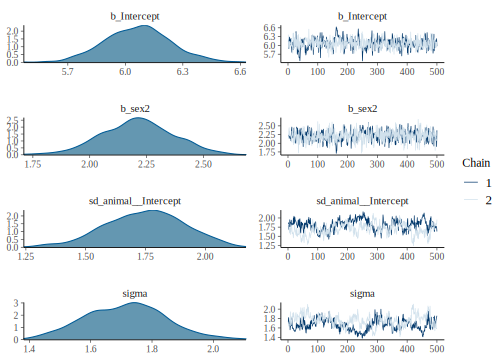
\includegraphics{wam_tuto_files/figure-latex/unnamed-chunk-56-1.pdf}

\begin{Shaded}
\begin{Highlighting}[]
\KeywordTok{summary}\NormalTok{(brms\_m1}\FloatTok{.2}\NormalTok{)}\OperatorTok{$}\NormalTok{fixed}
\end{Highlighting}
\end{Shaded}

\begin{verbatim}
## Warning: Parts of the model have not converged (some Rhats are > 1.05). Be
## careful when analysing the results! We recommend running more iterations and/or
## setting stronger priors.
\end{verbatim}

\begin{verbatim}
##           Estimate Est.Error l-95% CI u-95% CI     Rhat Bulk_ESS Tail_ESS
## Intercept 6.064853 0.1726459 5.735170 6.410117 1.002990 357.5666 574.2620
## sex2      2.210675 0.1574542 1.898645 2.520026 1.002313 722.8016 657.2121
\end{verbatim}

\begin{Shaded}
\begin{Highlighting}[]
\KeywordTok{summary}\NormalTok{(brms\_m1}\FloatTok{.2}\NormalTok{)}\OperatorTok{$}\NormalTok{random}
\end{Highlighting}
\end{Shaded}

\begin{verbatim}
## Warning: Parts of the model have not converged (some Rhats are > 1.05). Be
## careful when analysing the results! We recommend running more iterations and/or
## setting stronger priors.
\end{verbatim}

\begin{verbatim}
## $animal
##               Estimate Est.Error l-95% CI u-95% CI     Rhat Bulk_ESS Tail_ESS
## sd(Intercept) 1.747083 0.1632548 1.419377 2.050884 1.126639 13.10221 113.2445
\end{verbatim}

\hypertarget{adding-random-effects-2}{%
\subsection{Adding random effects}\label{adding-random-effects-2}}

This is done by simply modifying the model statement in the same way, but requires addition of a prior for the new random effect. For instance, we can fit an effect of birth year:

\begin{Shaded}
\begin{Highlighting}[]
\NormalTok{brms\_m1}\FloatTok{.3}\NormalTok{ \textless{}{-}}\StringTok{ }\KeywordTok{brm}\NormalTok{(}
\NormalTok{  bwt }\OperatorTok{\textasciitilde{}}\StringTok{ }\DecValTok{1} \OperatorTok{+}\StringTok{ }\NormalTok{sex }\OperatorTok{+}\StringTok{ }\NormalTok{(}\DecValTok{1} \OperatorTok{|}\StringTok{ }\KeywordTok{gr}\NormalTok{(animal, }\DataTypeTok{cov =}\NormalTok{ Amat)) }\OperatorTok{+}\StringTok{ }\NormalTok{(}\DecValTok{1} \OperatorTok{|}\StringTok{ }\NormalTok{byear) }\OperatorTok{+}\StringTok{ }\NormalTok{(}\DecValTok{1} \OperatorTok{|}\StringTok{ }\NormalTok{mother),}
  \DataTypeTok{data =}\NormalTok{ gryphon,}
  \DataTypeTok{data2 =} \KeywordTok{list}\NormalTok{(}\DataTypeTok{Amat =}\NormalTok{ Amat),}
  \DataTypeTok{family =} \KeywordTok{gaussian}\NormalTok{(),}
  \DataTypeTok{chains =} \DecValTok{2}\NormalTok{, }\DataTypeTok{cores =} \DecValTok{2}\NormalTok{, }\DataTypeTok{iter =} \DecValTok{1000}
\NormalTok{)}
\KeywordTok{save}\NormalTok{(brms\_m1}\FloatTok{.3}\NormalTok{, }\DataTypeTok{file =} \StringTok{"data/brms\_m1\_3.rda"}\NormalTok{)}
\end{Highlighting}
\end{Shaded}

\begin{Shaded}
\begin{Highlighting}[]
\KeywordTok{load}\NormalTok{(}\StringTok{"data/brms\_m1\_3.rda"}\NormalTok{)}
\KeywordTok{summary}\NormalTok{(brms\_m1}\FloatTok{.3}\NormalTok{)}
\end{Highlighting}
\end{Shaded}

\begin{verbatim}
## Warning: Parts of the model have not converged (some Rhats are > 1.05). Be
## careful when analysing the results! We recommend running more iterations and/or
## setting stronger priors.
\end{verbatim}

\begin{verbatim}
##  Family: gaussian 
##   Links: mu = identity; sigma = identity 
## Formula: bwt ~ 1 + sex + (1 | gr(animal, cov = Amat)) + (1 | byear) + (1 | mother) 
##    Data: gryphon (Number of observations: 854) 
##   Draws: 2 chains, each with iter = 1000; warmup = 500; thin = 1;
##          total post-warmup draws = 1000
## 
## Group-Level Effects: 
## ~animal (Number of levels: 854) 
##               Estimate Est.Error l-95% CI u-95% CI Rhat Bulk_ESS Tail_ESS
## sd(Intercept)     1.50      0.17     1.11     1.78 1.16        9       51
## 
## ~byear (Number of levels: 34) 
##               Estimate Est.Error l-95% CI u-95% CI Rhat Bulk_ESS Tail_ESS
## sd(Intercept)     0.96      0.14     0.71     1.28 1.00      400      642
## 
## ~mother (Number of levels: 394) 
##               Estimate Est.Error l-95% CI u-95% CI Rhat Bulk_ESS Tail_ESS
## sd(Intercept)     1.05      0.11     0.83     1.26 1.01      193      379
## 
## Population-Level Effects: 
##           Estimate Est.Error l-95% CI u-95% CI Rhat Bulk_ESS Tail_ESS
## Intercept     6.39      0.23     5.93     6.87 1.02      251      504
## sex2          1.97      0.15     1.67     2.28 1.00      644      785
## 
## Family Specific Parameters: 
##       Estimate Est.Error l-95% CI u-95% CI Rhat Bulk_ESS Tail_ESS
## sigma     1.30      0.14     1.03     1.56 1.17        9       55
## 
## Draws were sampled using sampling(NUTS). For each parameter, Bulk_ESS
## and Tail_ESS are effective sample size measures, and Rhat is the potential
## scale reduction factor on split chains (at convergence, Rhat = 1).
\end{verbatim}

\begin{Shaded}
\begin{Highlighting}[]
\KeywordTok{plot}\NormalTok{(brms\_m1}\FloatTok{.3}\NormalTok{, }\DataTypeTok{ask =} \OtherTok{FALSE}\NormalTok{, }\DataTypeTok{N =} \DecValTok{3}\NormalTok{)}
\end{Highlighting}
\end{Shaded}

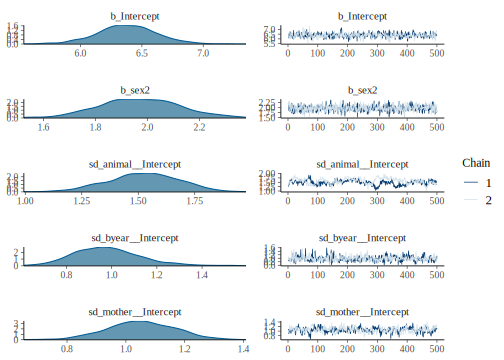
\includegraphics{wam_tuto_files/figure-latex/unnamed-chunk-58-1.pdf} 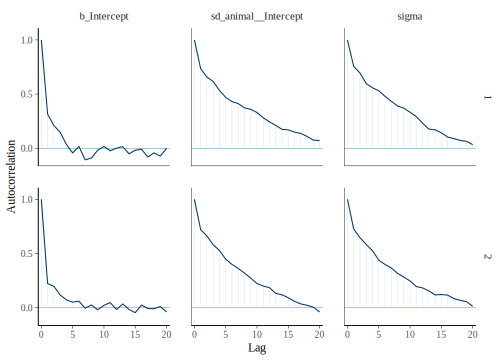
\includegraphics{wam_tuto_files/figure-latex/unnamed-chunk-58-2.pdf}

\hypertarget{testing-significance-of-variance-components-1}{%
\subsection{Testing significance of variance components}\label{testing-significance-of-variance-components-1}}

\hypertarget{further-partitioning-of-the-variance}{%
\subsection{Further partitioning of the variance}\label{further-partitioning-of-the-variance}}

Depending of the research question and the presence of different group within the dataset, MCMCglmm allowed to partition the variance at different level. For the example, we can partition the additive genetic and residual variance between SEXE (male and female) to estimate the sex-specific heritability

\begin{Shaded}
\begin{Highlighting}[]
\NormalTok{brms\_m1}\FloatTok{.4}\NormalTok{ \textless{}{-}}\StringTok{ }\KeywordTok{brm}\NormalTok{(}
\NormalTok{  bwt }\OperatorTok{\textasciitilde{}}\StringTok{ }\DecValTok{1} \OperatorTok{+}\StringTok{ }\NormalTok{sex }\OperatorTok{+}\StringTok{ }\NormalTok{(}\DecValTok{1} \OperatorTok{|}\StringTok{ }\KeywordTok{gr}\NormalTok{(animal, }\DataTypeTok{cov =}\NormalTok{ Amat)) }\OperatorTok{+}\StringTok{ }\NormalTok{(}\DecValTok{1} \OperatorTok{|}\StringTok{ }\NormalTok{byear) }\OperatorTok{+}\StringTok{ }\NormalTok{(}\DecValTok{1} \OperatorTok{|}\StringTok{ }\NormalTok{mother),}
  \DataTypeTok{data =}\NormalTok{ gryphon,}
  \DataTypeTok{data2 =} \KeywordTok{list}\NormalTok{(}\DataTypeTok{Amat =}\NormalTok{ Amat),}
  \DataTypeTok{family =} \KeywordTok{gaussian}\NormalTok{(),}
  \DataTypeTok{chains =} \DecValTok{2}\NormalTok{, }\DataTypeTok{cores =} \DecValTok{2}\NormalTok{, }\DataTypeTok{iter =} \DecValTok{1000}
\NormalTok{)}
\KeywordTok{save}\NormalTok{(brms\_m1}\FloatTok{.4}\NormalTok{, }\DataTypeTok{file =} \StringTok{"data/brms\_m1\_4.rda"}\NormalTok{)}
\end{Highlighting}
\end{Shaded}

\begin{Shaded}
\begin{Highlighting}[]
\KeywordTok{load}\NormalTok{(}\StringTok{"data/brms\_m1\_4.rda"}\NormalTok{)}
\KeywordTok{summary}\NormalTok{(brms\_m1}\FloatTok{.4}\NormalTok{)}
\end{Highlighting}
\end{Shaded}

\begin{verbatim}
## Warning: Parts of the model have not converged (some Rhats are > 1.05). Be
## careful when analysing the results! We recommend running more iterations and/or
## setting stronger priors.
\end{verbatim}

\begin{verbatim}
##  Family: gaussian 
##   Links: mu = identity; sigma = identity 
## Formula: bwt ~ 1 + sex + (1 | gr(animal, cov = Amat)) + (1 | byear) + (1 | mother) 
##    Data: gryphon (Number of observations: 854) 
##   Draws: 2 chains, each with iter = 1000; warmup = 500; thin = 1;
##          total post-warmup draws = 1000
## 
## Group-Level Effects: 
## ~animal (Number of levels: 854) 
##               Estimate Est.Error l-95% CI u-95% CI Rhat Bulk_ESS Tail_ESS
## sd(Intercept)     1.52      0.16     1.21     1.82 1.09       22      103
## 
## ~byear (Number of levels: 34) 
##               Estimate Est.Error l-95% CI u-95% CI Rhat Bulk_ESS Tail_ESS
## sd(Intercept)     0.98      0.15     0.73     1.32 1.00      538      677
## 
## ~mother (Number of levels: 394) 
##               Estimate Est.Error l-95% CI u-95% CI Rhat Bulk_ESS Tail_ESS
## sd(Intercept)     1.05      0.11     0.83     1.28 1.00      219      428
## 
## Population-Level Effects: 
##           Estimate Est.Error l-95% CI u-95% CI Rhat Bulk_ESS Tail_ESS
## Intercept     6.38      0.24     5.91     6.86 1.00      516      579
## sex2          1.97      0.15     1.68     2.28 1.00     1044      766
## 
## Family Specific Parameters: 
##       Estimate Est.Error l-95% CI u-95% CI Rhat Bulk_ESS Tail_ESS
## sigma     1.27      0.13     1.01     1.50 1.11       16       48
## 
## Draws were sampled using sampling(NUTS). For each parameter, Bulk_ESS
## and Tail_ESS are effective sample size measures, and Rhat is the potential
## scale reduction factor on split chains (at convergence, Rhat = 1).
\end{verbatim}

\begin{Shaded}
\begin{Highlighting}[]
\KeywordTok{plot}\NormalTok{(brms\_m1}\FloatTok{.4}\NormalTok{, }\DataTypeTok{ask =} \OtherTok{FALSE}\NormalTok{, }\DataTypeTok{N =} \DecValTok{3}\NormalTok{)}
\end{Highlighting}
\end{Shaded}

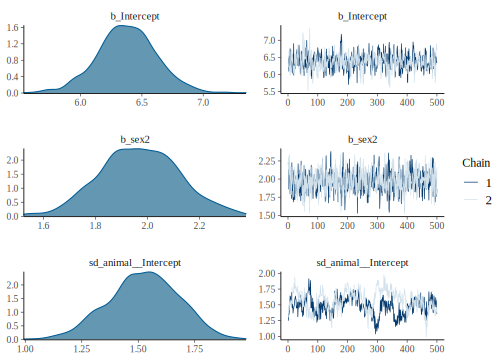
\includegraphics{wam_tuto_files/figure-latex/unnamed-chunk-60-1.pdf} 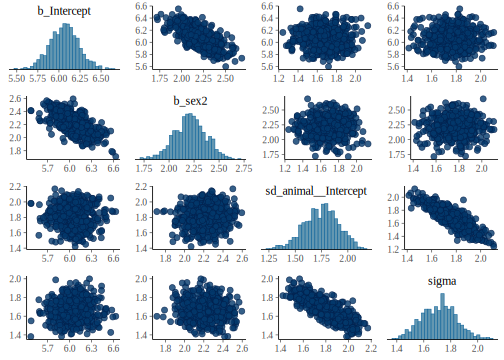
\includegraphics{wam_tuto_files/figure-latex/unnamed-chunk-60-2.pdf}

\hypertarget{modification-of-model-parameter-2}{%
\subsection{Modification of model parameter}\label{modification-of-model-parameter-2}}

\hypertarget{covariance-between-two-random-effects-2}{%
\subsection{Covariance between two random effects}\label{covariance-between-two-random-effects-2}}

\hypertarget{stan}{%
\section{stan}\label{stan}}

to do

\hypertarget{multivariate-animal-model}{%
\chapter{Multivariate animal model}\label{multivariate-animal-model}}

This tutorial will demonstrate how to run a multivariate animal model looking at birth weight and tarsus length of the phenomenal gryphons.

\hypertarget{scenario-and-data-1}{%
\section{Scenario and data}\label{scenario-and-data-1}}

\hypertarget{scenario-1}{%
\subsection{Scenario}\label{scenario-1}}

Since natural selection rarely acts on single traits, to understand how birth weight might evolve in our population of gryphons, we may also want to think about possible covariance with other traits. If tarsus length at fledging is also under positive selection, what implications does it have for birth weight and vice versa? If the two traits are positively genetically correlated then this will facilitate evolution of larger size (since response of one trait will induce a positively correlated response in the other). If there is negative genetic covariance then this could act as an evolutionary constraint.

Using multivariate models allows the estimation of parameters relating to each trait alone (\emph{i.e.} \(V_A\), \(h^2\), etc), but also yields estimates of covariance components between traits. These include the (additive) genetic covariance \(COV_A\) which is often rescaled to give the additive genetic correlation \(r_A\). However, covariance can also arise through other random effects (\emph{e.g.} maternal covariance) and these sources can also be explicitly modelled in a bivariate analysis.

\hypertarget{gryphon-files}{%
\subsection{gryphon files}\label{gryphon-files}}

gryphonpedigree and phenotypic data files are the same as those used in tutorial 1 (\emph{i.e}, \texttt{gryphonped.csv} and \texttt{gryphon.csv} respectively).

Reading the data

\begin{Shaded}
\begin{Highlighting}[]
\NormalTok{gryphon \textless{}{-}}\StringTok{ }\KeywordTok{read.csv}\NormalTok{(}\StringTok{"data/gryphon.csv"}\NormalTok{)}
\NormalTok{gryphon}\OperatorTok{$}\NormalTok{animal \textless{}{-}}\StringTok{ }\KeywordTok{as.factor}\NormalTok{(gryphon}\OperatorTok{$}\NormalTok{animal)}
\NormalTok{gryphon}\OperatorTok{$}\NormalTok{mother \textless{}{-}}\StringTok{ }\KeywordTok{as.factor}\NormalTok{(gryphon}\OperatorTok{$}\NormalTok{mother)}
\NormalTok{gryphon}\OperatorTok{$}\NormalTok{byear \textless{}{-}}\StringTok{ }\KeywordTok{as.factor}\NormalTok{(gryphon}\OperatorTok{$}\NormalTok{byear)}
\NormalTok{gryphon}\OperatorTok{$}\NormalTok{sex \textless{}{-}}\StringTok{ }\KeywordTok{as.factor}\NormalTok{(gryphon}\OperatorTok{$}\NormalTok{sex)}
\NormalTok{gryphon}\OperatorTok{$}\NormalTok{bwt \textless{}{-}}\StringTok{ }\KeywordTok{as.numeric}\NormalTok{(gryphon}\OperatorTok{$}\NormalTok{bwt)}
\NormalTok{gryphon}\OperatorTok{$}\NormalTok{tarsus \textless{}{-}}\StringTok{ }\KeywordTok{as.numeric}\NormalTok{(gryphon}\OperatorTok{$}\NormalTok{tarsus)}
\end{Highlighting}
\end{Shaded}

Reading the pedigree

\begin{Shaded}
\begin{Highlighting}[]
\NormalTok{gryphonped \textless{}{-}}\StringTok{ }\KeywordTok{read.csv}\NormalTok{(}\StringTok{"data/gryphonped.csv"}\NormalTok{)}
\NormalTok{gryphonped}\OperatorTok{$}\NormalTok{id \textless{}{-}}\StringTok{ }\KeywordTok{as.factor}\NormalTok{(gryphonped}\OperatorTok{$}\NormalTok{id)}
\NormalTok{gryphonped}\OperatorTok{$}\NormalTok{father \textless{}{-}}\StringTok{ }\KeywordTok{as.factor}\NormalTok{(gryphonped}\OperatorTok{$}\NormalTok{father)}
\NormalTok{gryphonped}\OperatorTok{$}\NormalTok{mother \textless{}{-}}\StringTok{ }\KeywordTok{as.factor}\NormalTok{(gryphonped}\OperatorTok{$}\NormalTok{mother)}
\end{Highlighting}
\end{Shaded}

\hypertarget{asreml-biv}{%
\section{Asreml-R}\label{asreml-biv}}

\hypertarget{running-the-model-3}{%
\subsection{Running the model}\label{running-the-model-3}}

First we need to load the \texttt{asreml} library:

\begin{Shaded}
\begin{Highlighting}[]
\KeywordTok{library}\NormalTok{(asreml)}
\end{Highlighting}
\end{Shaded}

For running multivariate analyses in ASReml-R, the code is slightly more complex than for the univariate case. This is because ASReml-R allows us to make different assumptions about the way in which traits might be related. So we need to explicitly code a model of the (co)variance structure we want to fit by specified some starting values. These are can be very approximate \emph{guestimates}, but having reasonable starting values can aid convergence. Finally, we have increased the default maximum number of iterations (\texttt{maxiter}) which can help to achieve convergence for more complicated models. Another way to increase the number of iteration will be to use the \texttt{update} function. Notes that if the \texttt{LogLik} is not stabilized after several iterations, it is good indication of the model require more iteration.

It is also possible to let the model running without any specify starting values but usually univariate model will allow to get some \emph{guestimates} in the additive genetic variances.

\begin{Shaded}
\begin{Highlighting}[]
\NormalTok{ainv \textless{}{-}}\StringTok{ }\KeywordTok{ainverse}\NormalTok{(gryphonped)}
\NormalTok{modela \textless{}{-}}\StringTok{ }\KeywordTok{asreml}\NormalTok{(}
  \DataTypeTok{fixed =} \KeywordTok{cbind}\NormalTok{(bwt, tarsus) }\OperatorTok{\textasciitilde{}}\StringTok{ }\NormalTok{trait,}
  \DataTypeTok{random =} \OperatorTok{\textasciitilde{}}\StringTok{ }\KeywordTok{us}\NormalTok{(trait)}\OperatorTok{:}\KeywordTok{vm}\NormalTok{(animal, ainv), }\DataTypeTok{init =} \KeywordTok{c}\NormalTok{(}\DecValTok{1}\NormalTok{, }\FloatTok{0.1}\NormalTok{, }\DecValTok{1}\NormalTok{),}
  \DataTypeTok{residual =} \OperatorTok{\textasciitilde{}}\StringTok{ }\KeywordTok{id}\NormalTok{(units)}\OperatorTok{:}\KeywordTok{us}\NormalTok{(trait, }\DataTypeTok{init =} \KeywordTok{c}\NormalTok{(}\DecValTok{1}\NormalTok{, }\FloatTok{0.1}\NormalTok{, }\DecValTok{1}\NormalTok{)),}
  \DataTypeTok{data =}\NormalTok{ gryphon,}
  \DataTypeTok{na.action =} \KeywordTok{na.method}\NormalTok{(}\DataTypeTok{x =} \StringTok{"include"}\NormalTok{, }\DataTypeTok{y =} \StringTok{"include"}\NormalTok{),}
  \DataTypeTok{maxit =} \DecValTok{20}
\NormalTok{)}
\end{Highlighting}
\end{Shaded}

\begin{verbatim}
## Warning in type.convert.default(x): 'as.is' should be specified by the caller;
## using TRUE

## Warning in type.convert.default(x): 'as.is' should be specified by the caller;
## using TRUE
\end{verbatim}

\begin{verbatim}
## Model fitted using the sigma parameterization.
## ASReml 4.1.0 Tue Nov 23 22:10:54 2021
##           LogLik        Sigma2     DF     wall    cpu
##  1     -5118.122           1.0   1535 22:10:54    0.0
##  2     -4358.769           1.0   1535 22:10:54    0.0
##  3     -3540.792           1.0   1535 22:10:54    0.0
##  4     -3004.970           1.0   1535 22:10:54    0.0
##  5     -2747.831           1.0   1535 22:10:54    0.0
##  6     -2687.807           1.0   1535 22:10:54    0.0
##  7     -2680.057           1.0   1535 22:10:54    0.0
##  8     -2679.743           1.0   1535 22:10:54    0.0
##  9     -2679.741           1.0   1535 22:10:54    0.0
\end{verbatim}

\begin{Shaded}
\begin{Highlighting}[]
\NormalTok{modela \textless{}{-}}\StringTok{ }\KeywordTok{update}\NormalTok{(modela)}
\end{Highlighting}
\end{Shaded}

\begin{verbatim}
## Warning in type.convert.default(x): 'as.is' should be specified by the caller;
## using TRUE

## Warning in type.convert.default(x): 'as.is' should be specified by the caller;
## using TRUE
\end{verbatim}

\begin{verbatim}
## Model fitted using the sigma parameterization.
## ASReml 4.1.0 Tue Nov 23 22:10:54 2021
##           LogLik        Sigma2     DF     wall    cpu
##  1     -2679.741           1.0   1535 22:10:55    0.0
##  2     -2679.741           1.0   1535 22:10:55    0.0
\end{verbatim}

\texttt{modela} has fitted a bivariate model of \texttt{bwt} and \texttt{tarsus}, with the mean for each of the traits as a fixed effect (\texttt{trait}). The additive genetic variance-covariance matrix (\(\textbf{G}\)) is unstructured (\texttt{us}; \emph{i.e.} all elements are free to vary) and the starting values for \(V_A\) for \texttt{bwt}, \(COV_A\) between \texttt{bwt} and \texttt{tarsus}, and \(V_A\) for \texttt{tarsus} are set to 1, 0.1 and 1, respectively. Similarly, the residual matrix is unstructured and uses the same starting values.

Note that the argument \texttt{na.action\ =\ na.method(x\ =\ "include",\ y\ =\ "include")} can be added to the model. In a bivariate model, it will help calculate the covariance between two traits with different missing information \texttt{NA} and so help imbalance phenotypage and save sample size. However, it is important to scale ( mean =0, var =1) the two traits to correctly adjust the model(see Asreml-R manual for more information).

Let's have a look at the variance components, and notice that there are now seven (co)variance components reported in the table:

\begin{Shaded}
\begin{Highlighting}[]
\KeywordTok{summary}\NormalTok{(modela)}\OperatorTok{$}\NormalTok{varcomp}
\end{Highlighting}
\end{Shaded}

\begin{verbatim}
##                                            component std.error  z.ratio bound
## trait:vm(animal, ainv)!trait_bwt:bwt        3.368405 0.6348356 5.305948     P
## trait:vm(animal, ainv)!trait_tarsus:bwt     2.459827 1.0732809 2.291876     P
## trait:vm(animal, ainv)!trait_tarsus:tarsus 12.345849 3.0744787 4.015591     P
## units:trait!R                               1.000000        NA       NA     F
## units:trait!trait_bwt:bwt                   3.849910 0.5200095 7.403539     P
## units:trait!trait_tarsus:bwt                3.313269 0.9129222 3.629300     P
## units:trait!trait_tarsus:tarsus            17.646386 2.6670308 6.616491     P
##                                            %ch
## trait:vm(animal, ainv)!trait_bwt:bwt         0
## trait:vm(animal, ainv)!trait_tarsus:bwt      0
## trait:vm(animal, ainv)!trait_tarsus:tarsus   0
## units:trait!R                                0
## units:trait!trait_bwt:bwt                    0
## units:trait!trait_tarsus:bwt                 0
## units:trait!trait_tarsus:tarsus              0
\end{verbatim}

The first three terms are related to the genetic matrix and, in order are \(V_{A,bwt}\), \(COV_A\), \(V_{A, tarsus}\). Below is again a line where the \texttt{units:traitr!R} component equals to 1, which again can be ignored. The final three terms relate to the residual matrix and correspond to \(V_{R,bwt}\), \(COV_R\), \(V_{R,tarsus}\). Based on our quick and dirty check (is \texttt{z.ratio} \textgreater{} 1.96?) all components look to be statistically significant.

We can calculate the genetic correlation as \(COV_A / \sqrt{V_{A,bwt} \cdot V_{A,tarsus}}\). Thus this model gives an estimate of \(r_A\) = 0.38. It is also possible to estimate the residual correlation \(r_res\) = 0.4.

Although we can calculate this by hand, we can also use \texttt{vpredict()}, which also provides an (approximate) standard error:

\begin{Shaded}
\begin{Highlighting}[]
\KeywordTok{vpredict}\NormalTok{(modela, r\_A }\OperatorTok{\textasciitilde{}}\StringTok{ }\NormalTok{V2 }\OperatorTok{/}\StringTok{ }\KeywordTok{sqrt}\NormalTok{(V1 }\OperatorTok{*}\StringTok{ }\NormalTok{V3))}
\end{Highlighting}
\end{Shaded}

\begin{verbatim}
##     Estimate        SE
## r_A 0.381445 0.1299765
\end{verbatim}

\begin{Shaded}
\begin{Highlighting}[]
\KeywordTok{vpredict}\NormalTok{(modela, r\_res }\OperatorTok{\textasciitilde{}}\StringTok{ }\NormalTok{V6 }\OperatorTok{/}\StringTok{ }\KeywordTok{sqrt}\NormalTok{(V5 }\OperatorTok{*}\StringTok{ }\NormalTok{V7))}
\end{Highlighting}
\end{Shaded}

\begin{verbatim}
##        Estimate         SE
## r_res 0.4019791 0.08607119
\end{verbatim}

Of course we can also calculate the heritability of \texttt{bwt} and \texttt{tarsus} from this model:

\begin{Shaded}
\begin{Highlighting}[]
\KeywordTok{vpredict}\NormalTok{(modela, h2.bwt }\OperatorTok{\textasciitilde{}}\StringTok{ }\NormalTok{V1 }\OperatorTok{/}\StringTok{ }\NormalTok{(V1 }\OperatorTok{+}\StringTok{ }\NormalTok{V5))}
\end{Highlighting}
\end{Shaded}

\begin{verbatim}
##         Estimate         SE
## h2.bwt 0.4666469 0.07671563
\end{verbatim}

\begin{Shaded}
\begin{Highlighting}[]
\KeywordTok{vpredict}\NormalTok{(modela, h2.tarsus }\OperatorTok{\textasciitilde{}}\StringTok{ }\NormalTok{V3 }\OperatorTok{/}\StringTok{ }\NormalTok{(V3 }\OperatorTok{+}\StringTok{ }\NormalTok{V7))}
\end{Highlighting}
\end{Shaded}

\begin{verbatim}
##            Estimate         SE
## h2.tarsus 0.4116348 0.09305947
\end{verbatim}

\hypertarget{adding-fixed-and-random-effects}{%
\subsection{Adding fixed and random effects}\label{adding-fixed-and-random-effects}}

Fixed and random effects can be added just as for the univariate case. Given that our full model of bwt from tutorial 1 had sex as a fixed effect as well as birth year and mother as random effects, we could specify a bivariate formulation with the same complexity:

\begin{Shaded}
\begin{Highlighting}[]
\NormalTok{modelb \textless{}{-}}\StringTok{ }\KeywordTok{asreml}\NormalTok{(}
  \DataTypeTok{fixed =} \KeywordTok{cbind}\NormalTok{(bwt, tarsus) }\OperatorTok{\textasciitilde{}}\StringTok{ }\NormalTok{trait }\OperatorTok{+}\StringTok{ }\KeywordTok{at}\NormalTok{(trait)}\OperatorTok{:}\NormalTok{sex,}
  \DataTypeTok{random =} \OperatorTok{\textasciitilde{}}\StringTok{ }\KeywordTok{us}\NormalTok{(trait, }\DataTypeTok{init =} \KeywordTok{c}\NormalTok{(}\DecValTok{1}\NormalTok{, }\FloatTok{0.1}\NormalTok{, }\DecValTok{1}\NormalTok{))}\OperatorTok{:}\KeywordTok{vm}\NormalTok{(animal, ainv) }\OperatorTok{+}
\StringTok{    }\KeywordTok{us}\NormalTok{(trait, }\DataTypeTok{init =} \KeywordTok{c}\NormalTok{(}\DecValTok{1}\NormalTok{, }\FloatTok{0.1}\NormalTok{, }\DecValTok{1}\NormalTok{))}\OperatorTok{:}\NormalTok{byear }\OperatorTok{+}
\StringTok{    }\KeywordTok{us}\NormalTok{(trait, }\DataTypeTok{init =} \KeywordTok{c}\NormalTok{(}\DecValTok{1}\NormalTok{, }\FloatTok{0.1}\NormalTok{, }\DecValTok{1}\NormalTok{))}\OperatorTok{:}\NormalTok{mother,}
  \DataTypeTok{residual =} \OperatorTok{\textasciitilde{}}\StringTok{ }\KeywordTok{id}\NormalTok{(units)}\OperatorTok{:}\KeywordTok{us}\NormalTok{(trait, }\DataTypeTok{init =} \KeywordTok{c}\NormalTok{(}\DecValTok{1}\NormalTok{, }\FloatTok{0.1}\NormalTok{, }\DecValTok{1}\NormalTok{)),}
  \DataTypeTok{data =}\NormalTok{ gryphon,}
  \DataTypeTok{na.action =} \KeywordTok{na.method}\NormalTok{(}\DataTypeTok{x =} \StringTok{"include"}\NormalTok{, }\DataTypeTok{y =} \StringTok{"include"}\NormalTok{),}
  \DataTypeTok{maxit =} \DecValTok{20}
\NormalTok{)}
\end{Highlighting}
\end{Shaded}

\begin{verbatim}
## Model fitted using the sigma parameterization.
## ASReml 4.1.0 Tue Nov 23 22:10:55 2021
##           LogLik        Sigma2     DF     wall    cpu
##  1     -4672.301           1.0   1533 22:10:55    0.0
##  2     -4005.615           1.0   1533 22:10:55    0.0
##  3     -3271.483           1.0   1533 22:10:55    0.0 (1 restrained)
##  4     -2761.414           1.0   1533 22:10:55    0.0 (1 restrained)
##  5     -2481.357           1.0   1533 22:10:55    0.0
##  6     -2395.858           1.0   1533 22:10:55    0.1
##  7     -2381.050           1.0   1533 22:10:55    0.0
##  8     -2380.251           1.0   1533 22:10:55    0.0
##  9     -2380.246           1.0   1533 22:10:55    0.0
\end{verbatim}

\begin{Shaded}
\begin{Highlighting}[]
\NormalTok{modelb \textless{}{-}}\StringTok{ }\KeywordTok{update}\NormalTok{(modelb)}
\end{Highlighting}
\end{Shaded}

\begin{verbatim}
## Model fitted using the sigma parameterization.
## ASReml 4.1.0 Tue Nov 23 22:10:55 2021
##           LogLik        Sigma2     DF     wall    cpu
##  1     -2380.246           1.0   1533 22:10:55    0.1
##  2     -2380.246           1.0   1533 22:10:55    0.0
\end{verbatim}

Note that we have specified a covariance structure for each random effect and an estimate of the effect of sex on both birth weight and tarsus length.

There will now be thirteen (co)variance components reported after running the code:

\begin{Shaded}
\begin{Highlighting}[]
\KeywordTok{summary}\NormalTok{(modelb)}\OperatorTok{$}\NormalTok{varcomp}
\end{Highlighting}
\end{Shaded}

\begin{verbatim}
##                                             component std.error    z.ratio
## trait:byear!trait_bwt:bwt                   0.9746385 0.2825727  3.4491602
## trait:byear!trait_tarsus:bwt                0.1624076 0.4185079  0.3880635
## trait:byear!trait_tarsus:tarsus             3.7383721 1.2065992  3.0982716
## trait:mother!trait_bwt:bwt                  1.1445184 0.2302182  4.9714512
## trait:mother!trait_tarsus:bwt              -1.5567306 0.4051848 -3.8420260
## trait:mother!trait_tarsus:tarsus            4.8206132 1.3201300  3.6516202
## trait:vm(animal, ainv)!trait_bwt:bwt        1.9893546 0.4410246  4.5107569
## trait:vm(animal, ainv)!trait_tarsus:bwt     3.3170404 0.9032323  3.6724110
## trait:vm(animal, ainv)!trait_tarsus:tarsus 10.2294887 2.8077066  3.6433610
## units:trait!R                               1.0000000        NA         NA
## units:trait!trait_bwt:bwt                   1.8443110 0.3443178  5.3564203
## units:trait!trait_tarsus:bwt                4.0142841 0.7412540  5.4155308
## units:trait!trait_tarsus:tarsus            12.4845955 2.2893363  5.4533690
##                                            bound %ch
## trait:byear!trait_bwt:bwt                      P   0
## trait:byear!trait_tarsus:bwt                   P   0
## trait:byear!trait_tarsus:tarsus                P   0
## trait:mother!trait_bwt:bwt                     P   0
## trait:mother!trait_tarsus:bwt                  P   0
## trait:mother!trait_tarsus:tarsus               P   0
## trait:vm(animal, ainv)!trait_bwt:bwt           P   0
## trait:vm(animal, ainv)!trait_tarsus:bwt        P   0
## trait:vm(animal, ainv)!trait_tarsus:tarsus     P   0
## units:trait!R                                  F   0
## units:trait!trait_bwt:bwt                      P   0
## units:trait!trait_tarsus:bwt                   P   0
## units:trait!trait_tarsus:tarsus                P   0
\end{verbatim}

we can estimate the different correlations using \texttt{vpredict}:

\begin{Shaded}
\begin{Highlighting}[]
\KeywordTok{vpredict}\NormalTok{(modelb, r\_byear }\OperatorTok{\textasciitilde{}}\StringTok{ }\NormalTok{V2 }\OperatorTok{/}\StringTok{ }\KeywordTok{sqrt}\NormalTok{(V1 }\OperatorTok{*}\StringTok{ }\NormalTok{V3))}
\end{Highlighting}
\end{Shaded}

\begin{verbatim}
##           Estimate        SE
## r_byear 0.08508312 0.2134209
\end{verbatim}

\begin{Shaded}
\begin{Highlighting}[]
\KeywordTok{vpredict}\NormalTok{(modelb, r\_M }\OperatorTok{\textasciitilde{}}\StringTok{ }\NormalTok{V5 }\OperatorTok{/}\StringTok{ }\KeywordTok{sqrt}\NormalTok{(V4 }\OperatorTok{*}\StringTok{ }\NormalTok{V6))}
\end{Highlighting}
\end{Shaded}

\begin{verbatim}
##       Estimate        SE
## r_M -0.6627518 0.2487963
\end{verbatim}

\begin{Shaded}
\begin{Highlighting}[]
\KeywordTok{vpredict}\NormalTok{(modelb, r\_A }\OperatorTok{\textasciitilde{}}\StringTok{ }\NormalTok{V8 }\OperatorTok{/}\StringTok{ }\KeywordTok{sqrt}\NormalTok{(V7 }\OperatorTok{*}\StringTok{ }\NormalTok{V9))}
\end{Highlighting}
\end{Shaded}

\begin{verbatim}
##      Estimate        SE
## r_A 0.7353053 0.1094747
\end{verbatim}

\begin{Shaded}
\begin{Highlighting}[]
\KeywordTok{vpredict}\NormalTok{(modelb, r\_res }\OperatorTok{\textasciitilde{}}\StringTok{ }\NormalTok{V12 }\OperatorTok{/}\StringTok{ }\KeywordTok{sqrt}\NormalTok{(V11 }\OperatorTok{*}\StringTok{ }\NormalTok{V13))}
\end{Highlighting}
\end{Shaded}

\begin{verbatim}
##        Estimate         SE
## r_res 0.8365729 0.07366762
\end{verbatim}

Now we can look at the fixed effects parameters and assess their significance with a conditional Wald F-test:

\begin{Shaded}
\begin{Highlighting}[]
\KeywordTok{summary}\NormalTok{(modelb, }\DataTypeTok{coef =} \OtherTok{TRUE}\NormalTok{)}\OperatorTok{$}\NormalTok{coef.fi}
\KeywordTok{wald.asreml}\NormalTok{(modelb, }\DataTypeTok{denDF =} \StringTok{"default"}\NormalTok{, }\DataTypeTok{ssType =} \StringTok{"conditional"}\NormalTok{)}\OperatorTok{$}\NormalTok{Wald}
\end{Highlighting}
\end{Shaded}

\begin{verbatim}
##                           solution std error    z.ratio
## at(trait, tarsus):sex_1  0.0000000        NA         NA
## at(trait, tarsus):sex_2 -0.0684413 0.3823448 -0.1790041
## at(trait, bwt):sex_1     0.0000000        NA         NA
## at(trait, bwt):sex_2     1.9502053 0.1480467 13.1729086
## trait_bwt                6.3844483 0.2328210 27.4221324
## trait_tarsus            20.5936436 0.5098944 40.3880569
\end{verbatim}

\begin{verbatim}
## Model fitted using the sigma parameterization.
## ASReml 4.1.0 Tue Nov 23 22:10:55 2021
##           LogLik        Sigma2     DF     wall    cpu
##  1     -2380.246           1.0   1533 22:10:56    0.1
##  2     -2380.246           1.0   1533 22:10:56    0.0
## Calculating denominator DF
\end{verbatim}

\begin{verbatim}
## 
##                       Df denDF   F.inc   F.con Margin      Pr
## trait                  2  52.6 1396.00 1396.00        0.00000
## at(trait, bwt):sex     1 812.8  298.40  173.50      B 0.00000
## at(trait, tarsus):sex  1 747.9    0.03    0.03      B 0.85798
\end{verbatim}

Note that it is possible to specify a fixed effect to a specific trait by adding the number of order within \texttt{cbind} inside the argument \texttt{at(trait,x)}. For example, here we apply the fixed effect \texttt{sex} only to the response variable \texttt{tarsus}.

\begin{Shaded}
\begin{Highlighting}[]
\NormalTok{modelb\_}\DecValTok{2}\NormalTok{ \textless{}{-}}\StringTok{ }\KeywordTok{asreml}\NormalTok{(}
  \DataTypeTok{fixed =} \KeywordTok{cbind}\NormalTok{(bwt, tarsus) }\OperatorTok{\textasciitilde{}}\StringTok{ }\NormalTok{trait }\OperatorTok{+}\StringTok{ }\KeywordTok{at}\NormalTok{(trait, }\DecValTok{2}\NormalTok{)}\OperatorTok{:}\NormalTok{sex,}
  \DataTypeTok{random =} \OperatorTok{\textasciitilde{}}\StringTok{ }\KeywordTok{us}\NormalTok{(trait, }\DataTypeTok{init =} \KeywordTok{c}\NormalTok{(}\DecValTok{1}\NormalTok{, }\FloatTok{0.1}\NormalTok{, }\DecValTok{1}\NormalTok{))}\OperatorTok{:}\KeywordTok{vm}\NormalTok{(animal, ainv) }\OperatorTok{+}
\StringTok{    }\KeywordTok{us}\NormalTok{(trait, }\DataTypeTok{init =} \KeywordTok{c}\NormalTok{(}\DecValTok{1}\NormalTok{, }\FloatTok{0.1}\NormalTok{, }\DecValTok{1}\NormalTok{))}\OperatorTok{:}\NormalTok{byear }\OperatorTok{+}
\StringTok{    }\KeywordTok{us}\NormalTok{(trait, }\DataTypeTok{init =} \KeywordTok{c}\NormalTok{(}\DecValTok{1}\NormalTok{, }\FloatTok{0.1}\NormalTok{, }\DecValTok{1}\NormalTok{))}\OperatorTok{:}\NormalTok{mother,}
  \DataTypeTok{residual =} \OperatorTok{\textasciitilde{}}\StringTok{ }\KeywordTok{id}\NormalTok{(units)}\OperatorTok{:}\KeywordTok{us}\NormalTok{(trait, }\DataTypeTok{init =} \KeywordTok{c}\NormalTok{(}\DecValTok{1}\NormalTok{, }\FloatTok{0.1}\NormalTok{, }\DecValTok{1}\NormalTok{)),}
  \DataTypeTok{data =}\NormalTok{ gryphon,}
  \DataTypeTok{na.action =} \KeywordTok{na.method}\NormalTok{(}\DataTypeTok{x =} \StringTok{"include"}\NormalTok{, }\DataTypeTok{y =} \StringTok{"include"}\NormalTok{),}
  \DataTypeTok{maxit =} \DecValTok{20}
\NormalTok{)}
\end{Highlighting}
\end{Shaded}

\begin{verbatim}
## Model fitted using the sigma parameterization.
## ASReml 4.1.0 Tue Nov 23 22:10:56 2021
##           LogLik        Sigma2     DF     wall    cpu
##  1     -4810.563           1.0   1534 22:10:56    0.1
##  2     -4129.799           1.0   1534 22:10:56    0.0
##  3     -3382.529           1.0   1534 22:10:56    0.1 (1 restrained)
##  4     -2864.076           1.0   1534 22:10:56    0.1
##  5     -2574.891           1.0   1534 22:10:56    0.1
##  6     -2478.879           1.0   1534 22:10:56    0.1
##  7     -2458.305           1.0   1534 22:10:57    0.1
##  8     -2456.425           1.0   1534 22:10:57    0.0
##  9     -2456.377           1.0   1534 22:10:57    0.1
## 10     -2456.376           1.0   1534 22:10:57    0.0
\end{verbatim}

\begin{Shaded}
\begin{Highlighting}[]
\KeywordTok{summary}\NormalTok{(modelb\_}\DecValTok{2}\NormalTok{, }\DataTypeTok{coef =} \OtherTok{TRUE}\NormalTok{)}\OperatorTok{$}\NormalTok{coef.fi}
\KeywordTok{wald.asreml}\NormalTok{(modelb\_}\DecValTok{2}\NormalTok{, }\DataTypeTok{denDF =} \StringTok{"default"}\NormalTok{, }\DataTypeTok{ssType =} \StringTok{"conditional"}\NormalTok{)}\OperatorTok{$}\NormalTok{Wald}
\end{Highlighting}
\end{Shaded}

\begin{verbatim}
##                          solution std error   z.ratio
## at(trait, tarsus):sex_1  0.000000        NA        NA
## at(trait, tarsus):sex_2 -3.267042 0.2953279 -11.06242
## trait_bwt                7.636226 0.2389515  31.95722
## trait_tarsus            22.703658 0.4827348  47.03133
\end{verbatim}

\begin{verbatim}
## Model fitted using the sigma parameterization.
## ASReml 4.1.0 Tue Nov 23 22:10:57 2021
##           LogLik        Sigma2     DF     wall    cpu
##  1     -2456.376           1.0   1534 22:10:57    0.1
##  2     -2456.376           1.0   1534 22:10:57    0.1
## Calculating denominator DF
\end{verbatim}

\begin{verbatim}
## 
##                       Df denDF  F.inc  F.con Margin          Pr
## trait                  2  50.7 1233.0 1233.0        0.00000e+00
## at(trait, tarsus):sex  1 522.9  122.4  122.4      B 1.02886e-25
\end{verbatim}

\hypertarget{significance-testing}{%
\subsection{Significance testing}\label{significance-testing}}

Under the model above \(r_M\) is estimated as -0.66 and the \texttt{z.ratio} associated with the corresponding covariance (\(COV_M\)) is \textgreater2 (in absolute terms). We might therefore infer that there is evidence for a strong negative correlation between the traits with respect to the mother and that while maternal identity explains variance in both traits those mothers that tend to produce heavier offspring actually tend to produce offspring with shorter tarsus lengths.

To formally test if \(COV_M\) is significantly different from zero, we can compare the log-likelihood for this model:

\begin{Shaded}
\begin{Highlighting}[]
\NormalTok{modelb}\OperatorTok{$}\NormalTok{loglik}
\end{Highlighting}
\end{Shaded}

\begin{verbatim}
## [1] -2380.246
\end{verbatim}

to a model in which we specify that \(COV_M\)=0. Since this constraint reduces the number of parameters to be estimated by one, we can use a likelihood ratio test (LRT) with one degree of freedom. To run the constrained model, we modify the G structure defined for the \texttt{mother} random effect to diagonal (\texttt{diag}), which means we only estimate the variances (the diagonal of the matrix) but not the covariance (the covariance are fixed to 0):

\begin{Shaded}
\begin{Highlighting}[]
\NormalTok{modelc \textless{}{-}}\StringTok{ }\KeywordTok{asreml}\NormalTok{(}
  \DataTypeTok{fixed =} \KeywordTok{cbind}\NormalTok{(bwt, tarsus) }\OperatorTok{\textasciitilde{}}\StringTok{ }\NormalTok{trait }\OperatorTok{+}\StringTok{ }\KeywordTok{at}\NormalTok{(trait)}\OperatorTok{:}\NormalTok{sex,}
  \DataTypeTok{random =} \OperatorTok{\textasciitilde{}}\StringTok{ }\KeywordTok{us}\NormalTok{(trait, }\DataTypeTok{init =} \KeywordTok{c}\NormalTok{(}\DecValTok{1}\NormalTok{, }\FloatTok{0.1}\NormalTok{, }\DecValTok{1}\NormalTok{))}\OperatorTok{:}\KeywordTok{vm}\NormalTok{(animal, ainv) }\OperatorTok{+}
\StringTok{    }\KeywordTok{us}\NormalTok{(trait, }\DataTypeTok{init =} \KeywordTok{c}\NormalTok{(}\DecValTok{1}\NormalTok{, }\FloatTok{0.1}\NormalTok{, }\DecValTok{1}\NormalTok{))}\OperatorTok{:}\NormalTok{byear }\OperatorTok{+}
\StringTok{    }\KeywordTok{diag}\NormalTok{(trait, }\DataTypeTok{init =} \KeywordTok{c}\NormalTok{(}\DecValTok{1}\NormalTok{, }\DecValTok{1}\NormalTok{))}\OperatorTok{:}\NormalTok{mother,}
  \DataTypeTok{residual =} \OperatorTok{\textasciitilde{}}\StringTok{ }\KeywordTok{id}\NormalTok{(units)}\OperatorTok{:}\KeywordTok{us}\NormalTok{(trait, }\DataTypeTok{init =} \KeywordTok{c}\NormalTok{(}\DecValTok{1}\NormalTok{, }\FloatTok{0.1}\NormalTok{, }\DecValTok{1}\NormalTok{)),}
  \DataTypeTok{data =}\NormalTok{ gryphon,}
  \DataTypeTok{na.action =} \KeywordTok{na.method}\NormalTok{(}\DataTypeTok{x =} \StringTok{"include"}\NormalTok{, }\DataTypeTok{y =} \StringTok{"include"}\NormalTok{),}
  \DataTypeTok{maxit =} \DecValTok{20}
\NormalTok{)}
\end{Highlighting}
\end{Shaded}

\begin{verbatim}
## Model fitted using the sigma parameterization.
## ASReml 4.1.0 Tue Nov 23 22:10:57 2021
##           LogLik        Sigma2     DF     wall    cpu
##  1     -4677.820           1.0   1533 22:10:57    0.0
##  2     -4010.442           1.0   1533 22:10:57    0.0
##  3     -3275.409           1.0   1533 22:10:57    0.0
##  4     -2763.519           1.0   1533 22:10:57    0.0
##  5     -2483.732           1.0   1533 22:10:57    0.0
##  6     -2400.242           1.0   1533 22:10:57    0.0
##  7     -2386.663           1.0   1533 22:10:58    0.0
##  8     -2386.049           1.0   1533 22:10:58    0.0
##  9     -2386.045           1.0   1533 22:10:58    0.0
\end{verbatim}

You can run \texttt{summary(modelc)\$varcomp} to confirm this worked. We can now obtain the log-likelihood of this model and compare this to that of \texttt{modelb} using a likelihood ratio test:

\begin{Shaded}
\begin{Highlighting}[]
\NormalTok{modelc}\OperatorTok{$}\NormalTok{loglik}
\end{Highlighting}
\end{Shaded}

\begin{verbatim}
## [1] -2386.045
\end{verbatim}

We can see that the model log-likelihood is now -2386.05.
And comparing the models using a likelihood ratio test:

\begin{Shaded}
\begin{Highlighting}[]
\DecValTok{2} \OperatorTok{*}\StringTok{ }\NormalTok{(modelb}\OperatorTok{$}\NormalTok{loglik }\OperatorTok{{-}}\StringTok{ }\NormalTok{modelc}\OperatorTok{$}\NormalTok{loglik)}
\end{Highlighting}
\end{Shaded}

\begin{verbatim}
## [1] 11.59835
\end{verbatim}

So our chi-square test statistic is \(\chi^2_1\)= 11.6.
The p-value that goes with this is obtained by:

\begin{Shaded}
\begin{Highlighting}[]
\DecValTok{1} \OperatorTok{{-}}\StringTok{ }\KeywordTok{pchisq}\NormalTok{(}\DecValTok{2} \OperatorTok{*}\StringTok{ }\NormalTok{(modelb}\OperatorTok{$}\NormalTok{loglik }\OperatorTok{{-}}\StringTok{ }\NormalTok{modelc}\OperatorTok{$}\NormalTok{loglik), }\DecValTok{1}\NormalTok{)}
\end{Highlighting}
\end{Shaded}

\begin{verbatim}
## [1] 0.0006601037
\end{verbatim}

We would therefore conclude that the maternal covariance is significantly different from zero.

We could apply the same procedure to show that the residual (environmental) covariance and the genetic covariance estimates are significantly greater than zero (\emph{i.e.}, heavier individuals tend to have longer tarsus lengths). In contrast, we should find that the byear covariance between the two traits is non-significant.

\begin{Shaded}
\begin{Highlighting}[]
\NormalTok{modeld \textless{}{-}}\StringTok{ }\KeywordTok{asreml}\NormalTok{(}
  \DataTypeTok{fixed =} \KeywordTok{cbind}\NormalTok{(bwt, tarsus) }\OperatorTok{\textasciitilde{}}\StringTok{ }\NormalTok{trait }\OperatorTok{+}\StringTok{ }\KeywordTok{at}\NormalTok{(trait)}\OperatorTok{:}\NormalTok{sex,}
  \DataTypeTok{random =} \OperatorTok{\textasciitilde{}}\StringTok{ }\KeywordTok{us}\NormalTok{(trait, }\DataTypeTok{init =} \KeywordTok{c}\NormalTok{(}\DecValTok{1}\NormalTok{, }\FloatTok{0.1}\NormalTok{, }\DecValTok{1}\NormalTok{))}\OperatorTok{:}\KeywordTok{vm}\NormalTok{(animal, ainv) }\OperatorTok{+}
\StringTok{    }\KeywordTok{diag}\NormalTok{(trait, }\DataTypeTok{init =} \KeywordTok{c}\NormalTok{(}\DecValTok{1}\NormalTok{, }\DecValTok{1}\NormalTok{))}\OperatorTok{:}\NormalTok{byear }\OperatorTok{+}
\StringTok{    }\KeywordTok{us}\NormalTok{(trait, }\DataTypeTok{init =} \KeywordTok{c}\NormalTok{(}\DecValTok{1}\NormalTok{, }\FloatTok{0.1}\NormalTok{, }\DecValTok{1}\NormalTok{))}\OperatorTok{:}\NormalTok{mother,}
  \DataTypeTok{residual =} \OperatorTok{\textasciitilde{}}\StringTok{ }\KeywordTok{id}\NormalTok{(units)}\OperatorTok{:}\KeywordTok{us}\NormalTok{(trait, }\DataTypeTok{init =} \KeywordTok{c}\NormalTok{(}\DecValTok{1}\NormalTok{, }\FloatTok{0.1}\NormalTok{, }\DecValTok{1}\NormalTok{)),}
  \DataTypeTok{data =}\NormalTok{ gryphon,}
  \DataTypeTok{na.action =} \KeywordTok{na.method}\NormalTok{(}\DataTypeTok{x =} \StringTok{"include"}\NormalTok{, }\DataTypeTok{y =} \StringTok{"include"}\NormalTok{),}
  \DataTypeTok{maxit =} \DecValTok{20}
\NormalTok{)}
\end{Highlighting}
\end{Shaded}

\begin{verbatim}
## Model fitted using the sigma parameterization.
## ASReml 4.1.0 Tue Nov 23 22:10:58 2021
##           LogLik        Sigma2     DF     wall    cpu
##  1     -4672.708           1.0   1533 22:10:58    0.0
##  2     -4005.953           1.0   1533 22:10:58    0.0
##  3     -3271.737           1.0   1533 22:10:58    0.0 (1 restrained)
##  4     -2761.626           1.0   1533 22:10:58    0.0 (1 restrained)
##  5     -2481.649           1.0   1533 22:10:58    0.0
##  6     -2395.992           1.0   1533 22:10:58    0.0
##  7     -2381.136           1.0   1533 22:10:58    0.0
##  8     -2380.331           1.0   1533 22:10:58    0.0
##  9     -2380.326           1.0   1533 22:10:58    0.0
\end{verbatim}

\begin{Shaded}
\begin{Highlighting}[]
\DecValTok{2} \OperatorTok{*}\StringTok{ }\NormalTok{(modelb}\OperatorTok{$}\NormalTok{loglik }\OperatorTok{{-}}\StringTok{ }\NormalTok{modeld}\OperatorTok{$}\NormalTok{loglik)}
\end{Highlighting}
\end{Shaded}

\begin{verbatim}
## [1] 0.1600641
\end{verbatim}

\begin{Shaded}
\begin{Highlighting}[]
\DecValTok{1} \OperatorTok{{-}}\StringTok{ }\KeywordTok{pchisq}\NormalTok{(}\DecValTok{2} \OperatorTok{*}\StringTok{ }\NormalTok{(modelb}\OperatorTok{$}\NormalTok{loglik }\OperatorTok{{-}}\StringTok{ }\NormalTok{modeld}\OperatorTok{$}\NormalTok{loglik), }\DecValTok{1}\NormalTok{)}
\end{Highlighting}
\end{Shaded}

\begin{verbatim}
## [1] 0.6890975
\end{verbatim}

\hypertarget{estimate-directly-the-genetic-correlation-within-the-model}{%
\subsection{Estimate directly the genetic correlation within the model}\label{estimate-directly-the-genetic-correlation-within-the-model}}

Within Asreml-r, different matrix structure can be specify such as \texttt{us},\texttt{corg}, \texttt{diag}, etc (cf see the Asreml-r guide). Instead of the fitting an unstructured matrix with the argument \texttt{us} or a reduced model with no covariance with the argument \texttt{diag}, we can also directly estimate the genetic correlation between the \texttt{bwt} and \texttt{tarsus} with \texttt{corgh}.
Here we decide to estimate directly the additive genetic correlation.

\begin{Shaded}
\begin{Highlighting}[]
\NormalTok{modele \textless{}{-}}\StringTok{ }\KeywordTok{asreml}\NormalTok{(}
  \DataTypeTok{fixed =} \KeywordTok{cbind}\NormalTok{(bwt, tarsus) }\OperatorTok{\textasciitilde{}}\StringTok{ }\NormalTok{trait }\OperatorTok{+}\StringTok{ }\KeywordTok{at}\NormalTok{(trait)}\OperatorTok{:}\NormalTok{sex,}
  \DataTypeTok{random =} \OperatorTok{\textasciitilde{}}\StringTok{ }\KeywordTok{corgh}\NormalTok{(trait)}\OperatorTok{:}\KeywordTok{vm}\NormalTok{(animal, ainv) }\OperatorTok{+}
\StringTok{    }\KeywordTok{us}\NormalTok{(trait, }\DataTypeTok{init =} \KeywordTok{c}\NormalTok{(}\DecValTok{1}\NormalTok{, }\FloatTok{0.1}\NormalTok{, }\DecValTok{1}\NormalTok{))}\OperatorTok{:}\NormalTok{byear }\OperatorTok{+}
\StringTok{    }\KeywordTok{us}\NormalTok{(trait, }\DataTypeTok{init =} \KeywordTok{c}\NormalTok{(}\DecValTok{1}\NormalTok{, }\FloatTok{0.1}\NormalTok{, }\DecValTok{1}\NormalTok{))}\OperatorTok{:}\NormalTok{mother,}
  \DataTypeTok{residual =} \OperatorTok{\textasciitilde{}}\StringTok{ }\KeywordTok{id}\NormalTok{(units)}\OperatorTok{:}\KeywordTok{us}\NormalTok{(trait, }\DataTypeTok{init =} \KeywordTok{c}\NormalTok{(}\DecValTok{1}\NormalTok{, }\FloatTok{0.1}\NormalTok{, }\DecValTok{1}\NormalTok{)),}
  \DataTypeTok{data =}\NormalTok{ gryphon,}
  \DataTypeTok{na.action =} \KeywordTok{na.method}\NormalTok{(}\DataTypeTok{x =} \StringTok{"include"}\NormalTok{, }\DataTypeTok{y =} \StringTok{"include"}\NormalTok{),}
  \DataTypeTok{maxit =} \DecValTok{20}
\NormalTok{)}
\end{Highlighting}
\end{Shaded}

\begin{verbatim}
## Warning in type.convert.default(x): 'as.is' should be specified by the caller;
## using TRUE

## Warning in type.convert.default(x): 'as.is' should be specified by the caller;
## using TRUE
\end{verbatim}

\begin{verbatim}
## Model fitted using the sigma parameterization.
## ASReml 4.1.0 Tue Nov 23 22:10:58 2021
##           LogLik        Sigma2     DF     wall    cpu
##  1     -3544.356           1.0   1533 22:10:58    0.0
##  2     -3177.908           1.0   1533 22:10:58    0.0 (1 restrained)
##  3     -2784.992           1.0   1533 22:10:58    0.0
##  4     -2527.352           1.0   1533 22:10:58    0.0
##  5     -2406.422           1.0   1533 22:10:58    0.1
##  6     -2382.062           1.0   1533 22:10:58    0.0
##  7     -2380.263           1.0   1533 22:10:58    0.0
##  8     -2380.246           1.0   1533 22:10:58    0.0
##  9     -2380.246           1.0   1533 22:10:58    0.0
\end{verbatim}

\begin{Shaded}
\begin{Highlighting}[]
\NormalTok{modele \textless{}{-}}\StringTok{ }\KeywordTok{update}\NormalTok{(modele)}
\end{Highlighting}
\end{Shaded}

\begin{verbatim}
## Warning in type.convert.default(x): 'as.is' should be specified by the caller;
## using TRUE

## Warning in type.convert.default(x): 'as.is' should be specified by the caller;
## using TRUE
\end{verbatim}

\begin{verbatim}
## Model fitted using the sigma parameterization.
## ASReml 4.1.0 Tue Nov 23 22:10:58 2021
##           LogLik        Sigma2     DF     wall    cpu
##  1     -2380.246           1.0   1533 22:10:59    0.0
##  2     -2380.246           1.0   1533 22:10:59    0.0
\end{verbatim}

\begin{Shaded}
\begin{Highlighting}[]
\KeywordTok{summary}\NormalTok{(modele)}\OperatorTok{$}\NormalTok{varcomp}
\end{Highlighting}
\end{Shaded}

\begin{verbatim}
##                                                     component std.error
## trait:byear!trait_bwt:bwt                           0.9746376 0.2825690
## trait:byear!trait_tarsus:bwt                        0.1624052 0.4184989
## trait:byear!trait_tarsus:tarsus                     3.7383599 1.2065684
## trait:mother!trait_bwt:bwt                          1.1445196 0.2302189
## trait:mother!trait_tarsus:bwt                      -1.5567326 0.4051847
## trait:mother!trait_tarsus:tarsus                    4.8206100 1.3201239
## trait:vm(animal, ainv)!trait!tarsus:!trait!bwt.cor  0.7353034 0.1094744
## trait:vm(animal, ainv)!trait_bwt                    1.9893544 0.4410242
## trait:vm(animal, ainv)!trait_tarsus                10.2296667 2.8078190
## units:trait!R                                       1.0000000        NA
## units:trait!trait_bwt:bwt                           1.8443104 0.3443173
## units:trait!trait_tarsus:bwt                        4.0142731 0.7412587
## units:trait!trait_tarsus:tarsus                    12.4844745 2.2893621
##                                                      z.ratio bound %ch
## trait:byear!trait_bwt:bwt                           3.449203     P   0
## trait:byear!trait_tarsus:bwt                        0.388066     P   0
## trait:byear!trait_tarsus:tarsus                     3.098341     P   0
## trait:mother!trait_bwt:bwt                          4.971441     P   0
## trait:mother!trait_tarsus:bwt                      -3.842032     P   0
## trait:mother!trait_tarsus:tarsus                    3.651634     P   0
## trait:vm(animal, ainv)!trait!tarsus:!trait!bwt.cor  6.716668     U   0
## trait:vm(animal, ainv)!trait_bwt                    4.510760     P   0
## trait:vm(animal, ainv)!trait_tarsus                 3.643279     P   0
## units:trait!R                                             NA     F   0
## units:trait!trait_bwt:bwt                           5.356427     P   0
## units:trait!trait_tarsus:bwt                        5.415482     P   0
## units:trait!trait_tarsus:tarsus                     5.453255     P   0
\end{verbatim}

It is important to note that using \texttt{corgh} change the order of the estimate (co)variance. All different calculation need to be adjust in consequence.
It is also important to check the difference between the model with \texttt{us} and \texttt{corgh} to make sure any mistake are made.

\begin{Shaded}
\begin{Highlighting}[]
\KeywordTok{summary}\NormalTok{(modelb)}\OperatorTok{$}\NormalTok{loglik}
\end{Highlighting}
\end{Shaded}

\begin{verbatim}
## [1] -2380.246
\end{verbatim}

\begin{Shaded}
\begin{Highlighting}[]
\KeywordTok{summary}\NormalTok{(modele)}\OperatorTok{$}\NormalTok{loglik}
\end{Highlighting}
\end{Shaded}

\begin{verbatim}
## [1] -2380.246
\end{verbatim}

There two main advantages to use \texttt{corgh}: first, a direct estimation of correlation within the G matrix can avoid mistake in the \texttt{vpredict} calculation; second, it is possible to test if the correlation is significantly different than 0 (similar result as LRT with the covariance) but also to -1 and 1 which correspond of the correlation boundaries.
The following code showed how to create a reduced model with the correlation close to 1 and compared to the initial model.
Since we compared the correlation to its boundary, the degree of freedom is only half as a one tail LTR.

\begin{Shaded}
\begin{Highlighting}[]
\NormalTok{MODEL\_MODIF \textless{}{-}}\StringTok{ }\KeywordTok{update.asreml}\NormalTok{(modele, }\DataTypeTok{start.values =}\NormalTok{ T)}
\end{Highlighting}
\end{Shaded}

\begin{verbatim}
## Warning in type.convert.default(x): 'as.is' should be specified by the caller;
## using TRUE

## Warning in type.convert.default(x): 'as.is' should be specified by the caller;
## using TRUE
\end{verbatim}

\begin{Shaded}
\begin{Highlighting}[]
\NormalTok{G\_MOD \textless{}{-}}\StringTok{ }\NormalTok{MODEL\_MODIF}\OperatorTok{$}\NormalTok{vparameters.table[(}\DecValTok{1}\OperatorTok{:}\DecValTok{9}\NormalTok{), ]}
\NormalTok{G\_MOD[}\DecValTok{1}\NormalTok{, }\DecValTok{2}\NormalTok{] \textless{}{-}}\StringTok{ }\FloatTok{0.99999}
\NormalTok{G\_MOD[}\DecValTok{1}\NormalTok{, }\DecValTok{3}\NormalTok{] \textless{}{-}}\StringTok{ "F"}
\NormalTok{modele.red \textless{}{-}}\StringTok{ }\KeywordTok{asreml}\NormalTok{(}
  \DataTypeTok{fixed =} \KeywordTok{cbind}\NormalTok{(bwt, tarsus) }\OperatorTok{\textasciitilde{}}\StringTok{ }\NormalTok{trait }\OperatorTok{+}\StringTok{ }\KeywordTok{at}\NormalTok{(trait)}\OperatorTok{:}\NormalTok{sex,}
  \DataTypeTok{random =} \OperatorTok{\textasciitilde{}}\StringTok{ }\KeywordTok{corgh}\NormalTok{(trait)}\OperatorTok{:}\KeywordTok{vm}\NormalTok{(animal, ainv) }\OperatorTok{+}
\StringTok{    }\KeywordTok{us}\NormalTok{(trait, }\DataTypeTok{init =} \KeywordTok{c}\NormalTok{(}\DecValTok{1}\NormalTok{, }\FloatTok{0.1}\NormalTok{, }\DecValTok{1}\NormalTok{))}\OperatorTok{:}\NormalTok{byear }\OperatorTok{+}
\StringTok{    }\KeywordTok{us}\NormalTok{(trait, }\DataTypeTok{init =} \KeywordTok{c}\NormalTok{(}\DecValTok{1}\NormalTok{, }\FloatTok{0.1}\NormalTok{, }\DecValTok{1}\NormalTok{))}\OperatorTok{:}\NormalTok{mother,}
  \DataTypeTok{residual =} \OperatorTok{\textasciitilde{}}\StringTok{ }\KeywordTok{id}\NormalTok{(units)}\OperatorTok{:}\KeywordTok{us}\NormalTok{(trait, }\DataTypeTok{init =} \KeywordTok{c}\NormalTok{(}\DecValTok{1}\NormalTok{, }\FloatTok{0.1}\NormalTok{, }\DecValTok{1}\NormalTok{)),}
  \DataTypeTok{data =}\NormalTok{ gryphon,}
  \DataTypeTok{na.action =} \KeywordTok{na.method}\NormalTok{(}\DataTypeTok{x =} \StringTok{"include"}\NormalTok{, }\DataTypeTok{y =} \StringTok{"include"}\NormalTok{),}
  \DataTypeTok{maxit =} \DecValTok{20}\NormalTok{,}
  \DataTypeTok{G.param =}\NormalTok{ G\_MOD}
\NormalTok{)}
\end{Highlighting}
\end{Shaded}

\begin{verbatim}
## Warning in type.convert.default(x): 'as.is' should be specified by the caller;
## using TRUE

## Warning in type.convert.default(x): 'as.is' should be specified by the caller;
## using TRUE
\end{verbatim}

\begin{verbatim}
## Model fitted using the sigma parameterization.
## ASReml 4.1.0 Tue Nov 23 22:10:59 2021
##           LogLik        Sigma2     DF     wall    cpu
##  1     -2545.227           1.0   1533 22:10:59    0.0
##  2     -2483.880           1.0   1533 22:10:59    0.0
##  3     -2423.502           1.0   1533 22:10:59    0.0
##  4     -2392.508           1.0   1533 22:10:59    0.0
##  5     -2383.661           1.0   1533 22:10:59    0.0
##  6     -2383.084           1.0   1533 22:10:59    0.0
##  7     -2383.033           1.0   1533 22:10:59    0.0
##  8     -2383.022           1.0   1533 22:10:59    0.0
##  9     -2383.019           1.0   1533 22:10:59    0.0
## 10     -2383.019           1.0   1533 22:10:59    0.0
\end{verbatim}

\begin{Shaded}
\begin{Highlighting}[]
\DecValTok{2} \OperatorTok{*}\StringTok{ }\NormalTok{(modele}\OperatorTok{$}\NormalTok{loglik }\OperatorTok{{-}}\StringTok{ }\NormalTok{modele.red}\OperatorTok{$}\NormalTok{loglik)}
\end{Highlighting}
\end{Shaded}

\begin{verbatim}
## [1] 5.544679
\end{verbatim}

\begin{Shaded}
\begin{Highlighting}[]
\DecValTok{1} \OperatorTok{{-}}\StringTok{ }\KeywordTok{pchisq}\NormalTok{(}\DecValTok{2} \OperatorTok{*}\StringTok{ }\NormalTok{(modele}\OperatorTok{$}\NormalTok{loglik }\OperatorTok{{-}}\StringTok{ }\NormalTok{modele.red}\OperatorTok{$}\NormalTok{loglik), }\DataTypeTok{df =} \FloatTok{0.5}\NormalTok{)}
\end{Highlighting}
\end{Shaded}

\begin{verbatim}
## [1] 0.006598675
\end{verbatim}

Here, the correlation is significantly different than 1 (\textasciitilde0.99999).

\hypertarget{visualisation-of-the-correlation-aka-blup-extraction}{%
\subsection{Visualisation of the correlation (aka BLUP extraction)}\label{visualisation-of-the-correlation-aka-blup-extraction}}

When estimating correlation between traits, having a visualisation of it can help the interpretation. In addition, visualizing the correlation can spot outlier in the dataset.
Thanks to mixed model, each breeding values is stored within the model and can be extract as BLUP (Best Linear Unbiaised Predictor).
BLUP should be normaly distributed, if not you need to check the assumption of your animal model.extract

To simplify the following code, we rename the variable T1 and T2.

\begin{Shaded}
\begin{Highlighting}[]
\NormalTok{gryphon}\OperatorTok{$}\NormalTok{T1\textless{}{-}gryphon}\OperatorTok{$}\NormalTok{bwt}
\NormalTok{gryphon}\OperatorTok{$}\NormalTok{T2\textless{}{-}gryphon}\OperatorTok{$}\NormalTok{tarsus}
\CommentTok{\#\#\#\#\#\#\#\#\#\#\#\#}
\NormalTok{modele \textless{}{-}}\StringTok{ }\KeywordTok{asreml}\NormalTok{(}
  \DataTypeTok{fixed =} \KeywordTok{cbind}\NormalTok{(T1, T2) }\OperatorTok{\textasciitilde{}}\StringTok{ }\NormalTok{trait }\OperatorTok{+}\StringTok{ }\KeywordTok{at}\NormalTok{(trait)}\OperatorTok{:}\NormalTok{sex,}
  \DataTypeTok{random =} \OperatorTok{\textasciitilde{}}\StringTok{ }\KeywordTok{corgh}\NormalTok{(trait)}\OperatorTok{:}\KeywordTok{vm}\NormalTok{(animal, ainv) }\OperatorTok{+}
\StringTok{    }\KeywordTok{us}\NormalTok{(trait, }\DataTypeTok{init =} \KeywordTok{c}\NormalTok{(}\DecValTok{1}\NormalTok{, }\FloatTok{0.1}\NormalTok{, }\DecValTok{1}\NormalTok{))}\OperatorTok{:}\NormalTok{byear }\OperatorTok{+}
\StringTok{    }\KeywordTok{us}\NormalTok{(trait, }\DataTypeTok{init =} \KeywordTok{c}\NormalTok{(}\DecValTok{1}\NormalTok{, }\FloatTok{0.1}\NormalTok{, }\DecValTok{1}\NormalTok{))}\OperatorTok{:}\NormalTok{mother,}
  \DataTypeTok{residual =} \OperatorTok{\textasciitilde{}}\StringTok{ }\KeywordTok{id}\NormalTok{(units)}\OperatorTok{:}\KeywordTok{us}\NormalTok{(trait, }\DataTypeTok{init =} \KeywordTok{c}\NormalTok{(}\DecValTok{1}\NormalTok{, }\FloatTok{0.1}\NormalTok{, }\DecValTok{1}\NormalTok{)),}
  \DataTypeTok{data =}\NormalTok{ gryphon,}
  \DataTypeTok{na.action =} \KeywordTok{na.method}\NormalTok{(}\DataTypeTok{x =} \StringTok{"include"}\NormalTok{, }\DataTypeTok{y =} \StringTok{"include"}\NormalTok{),}
  \DataTypeTok{maxit =} \DecValTok{20}
\NormalTok{)}
\end{Highlighting}
\end{Shaded}

\begin{verbatim}
## Warning in type.convert.default(x): 'as.is' should be specified by the caller;
## using TRUE

## Warning in type.convert.default(x): 'as.is' should be specified by the caller;
## using TRUE
\end{verbatim}

\begin{verbatim}
## Model fitted using the sigma parameterization.
## ASReml 4.1.0 Tue Nov 23 22:10:59 2021
##           LogLik        Sigma2     DF     wall    cpu
##  1     -3544.356           1.0   1533 22:10:59    0.0
##  2     -3177.908           1.0   1533 22:10:59    0.0 (1 restrained)
##  3     -2784.992           1.0   1533 22:10:59    0.0
##  4     -2527.352           1.0   1533 22:10:59    0.0
##  5     -2406.422           1.0   1533 22:10:59    0.0
##  6     -2382.062           1.0   1533 22:10:59    0.0
##  7     -2380.263           1.0   1533 22:11:00    0.1
##  8     -2380.246           1.0   1533 22:11:00    0.0
##  9     -2380.246           1.0   1533 22:11:00    0.0
\end{verbatim}

\begin{Shaded}
\begin{Highlighting}[]
\NormalTok{modele \textless{}{-}}\StringTok{ }\KeywordTok{update}\NormalTok{(modele)}
\end{Highlighting}
\end{Shaded}

\begin{verbatim}
## Warning in type.convert.default(x): 'as.is' should be specified by the caller;
## using TRUE

## Warning in type.convert.default(x): 'as.is' should be specified by the caller;
## using TRUE
\end{verbatim}

\begin{verbatim}
## Model fitted using the sigma parameterization.
## ASReml 4.1.0 Tue Nov 23 22:11:00 2021
##           LogLik        Sigma2     DF     wall    cpu
##  1     -2380.246           1.0   1533 22:11:00    0.0
##  2     -2380.246           1.0   1533 22:11:00    0.0
\end{verbatim}

\begin{Shaded}
\begin{Highlighting}[]
\KeywordTok{summary}\NormalTok{(modele)}\OperatorTok{$}\NormalTok{varcomp}
\end{Highlighting}
\end{Shaded}

\begin{verbatim}
##                                                component std.error   z.ratio
## trait:byear!trait_T1:T1                        0.9746376 0.2825690  3.449203
## trait:byear!trait_T2:T1                        0.1624052 0.4184989  0.388066
## trait:byear!trait_T2:T2                        3.7383599 1.2065684  3.098341
## trait:mother!trait_T1:T1                       1.1445196 0.2302189  4.971441
## trait:mother!trait_T2:T1                      -1.5567326 0.4051847 -3.842032
## trait:mother!trait_T2:T2                       4.8206100 1.3201239  3.651634
## trait:vm(animal, ainv)!trait!T2:!trait!T1.cor  0.7353034 0.1094744  6.716668
## trait:vm(animal, ainv)!trait_T1                1.9893544 0.4410242  4.510760
## trait:vm(animal, ainv)!trait_T2               10.2296667 2.8078190  3.643279
## units:trait!R                                  1.0000000        NA        NA
## units:trait!trait_T1:T1                        1.8443104 0.3443173  5.356427
## units:trait!trait_T2:T1                        4.0142731 0.7412587  5.415482
## units:trait!trait_T2:T2                       12.4844745 2.2893621  5.453255
##                                               bound %ch
## trait:byear!trait_T1:T1                           P   0
## trait:byear!trait_T2:T1                           P   0
## trait:byear!trait_T2:T2                           P   0
## trait:mother!trait_T1:T1                          P   0
## trait:mother!trait_T2:T1                          P   0
## trait:mother!trait_T2:T2                          P   0
## trait:vm(animal, ainv)!trait!T2:!trait!T1.cor     U   0
## trait:vm(animal, ainv)!trait_T1                   P   0
## trait:vm(animal, ainv)!trait_T2                   P   0
## units:trait!R                                     F   0
## units:trait!trait_T1:T1                           P   0
## units:trait!trait_T2:T1                           P   0
## units:trait!trait_T2:T2                           P   0
\end{verbatim}

\begin{Shaded}
\begin{Highlighting}[]
\CommentTok{\#\#\#\#\#\#\#\#\#\#\#\#}
\NormalTok{DvsS\textless{}{-}}\KeywordTok{data.frame}\NormalTok{(}\DataTypeTok{Trait =} \KeywordTok{rownames}\NormalTok{(modele}\OperatorTok{$}\NormalTok{coefficients}\OperatorTok{$}\NormalTok{random),}
                 \DataTypeTok{BLUP =}\NormalTok{ modele}\OperatorTok{$}\NormalTok{coefficients}\OperatorTok{$}\NormalTok{random,}
                 \DataTypeTok{SE =} \KeywordTok{sqrt}\NormalTok{(modele}\OperatorTok{$}\NormalTok{vcoeff}\OperatorTok{$}\NormalTok{random}\OperatorTok{*}\NormalTok{modele}\OperatorTok{$}\NormalTok{sigma2))}
\NormalTok{DvsS}\OperatorTok{$}\NormalTok{ID\textless{}{-}}\KeywordTok{substr}\NormalTok{(DvsS}\OperatorTok{$}\NormalTok{Trait, }\DecValTok{27}\NormalTok{,}\DecValTok{30}\NormalTok{)}
\NormalTok{DvsS}\OperatorTok{$}\NormalTok{TRAIT\textless{}{-}}\KeywordTok{substr}\NormalTok{(DvsS}\OperatorTok{$}\NormalTok{Trait, }\DecValTok{7}\NormalTok{,}\DecValTok{8}\NormalTok{)}
\NormalTok{DvsS\textless{}{-}DvsS[}\DecValTok{927}\OperatorTok{:}\DecValTok{3544}\NormalTok{,] }\CommentTok{\#keep only row associated to animal }
\KeywordTok{summary}\NormalTok{(}\KeywordTok{factor}\NormalTok{(DvsS}\OperatorTok{$}\NormalTok{TRAIT)) }\CommentTok{\# 1309 each}
\end{Highlighting}
\end{Shaded}

\begin{verbatim}
##   T1   T2 
## 1309 1309
\end{verbatim}

\begin{Shaded}
\begin{Highlighting}[]
\CommentTok{\#}
\NormalTok{DvsS}\OperatorTok{$}\NormalTok{Trait\textless{}{-}}\OtherTok{NULL}
\KeywordTok{colnames}\NormalTok{(DvsS)[}\DecValTok{1}\NormalTok{]\textless{}{-}}\StringTok{"BLUP"}
\NormalTok{BLUPS\textless{}{-}}\KeywordTok{reshape}\NormalTok{(DvsS, }\DataTypeTok{v.names =} \KeywordTok{c}\NormalTok{(}\StringTok{"BLUP"}\NormalTok{,}\StringTok{"SE"}\NormalTok{), }\DataTypeTok{idvar =} \StringTok{"ID"}\NormalTok{,}\DataTypeTok{timevar =} \StringTok{"TRAIT"}\NormalTok{, }\DataTypeTok{direction =} \StringTok{"wide"}\NormalTok{)}
\KeywordTok{nrow}\NormalTok{(BLUPS)}
\end{Highlighting}
\end{Shaded}

\begin{verbatim}
## [1] 1309
\end{verbatim}

\begin{Shaded}
\begin{Highlighting}[]
\KeywordTok{rownames}\NormalTok{(BLUPS) \textless{}{-}}\StringTok{ }\KeywordTok{c}\NormalTok{()}
\KeywordTok{colnames}\NormalTok{(BLUPS) \textless{}{-}}\StringTok{ }\KeywordTok{c}\NormalTok{(}\StringTok{"ID"}\NormalTok{,}\StringTok{"BLUP.btw"}\NormalTok{,}\StringTok{"SE.btw"}\NormalTok{,}\StringTok{"BLUP.tarsus"}\NormalTok{,}\StringTok{"SE.tarsus"}\NormalTok{)}
\KeywordTok{summary}\NormalTok{(BLUPS)}
\end{Highlighting}
\end{Shaded}

\begin{verbatim}
##       ID               BLUP.btw             SE.btw        BLUP.tarsus      
##  Length:1309        Min.   :-3.165477   Min.   :0.7984   Min.   :-6.34167  
##  Class :character   1st Qu.:-0.559295   1st Qu.:0.9967   1st Qu.:-1.14433  
##  Mode  :character   Median :-0.001902   Median :1.0367   Median :-0.02629  
##                     Mean   :-0.009007   Mean   :1.0933   Mean   : 0.02134  
##                     3rd Qu.: 0.533983   3rd Qu.:1.2210   3rd Qu.: 1.18113  
##                     Max.   : 3.319620   Max.   :1.4377   Max.   : 6.71613  
##    SE.tarsus    
##  Min.   :1.928  
##  1st Qu.:2.371  
##  Median :2.451  
##  Mean   :2.577  
##  3rd Qu.:2.811  
##  Max.   :3.287
\end{verbatim}

\begin{Shaded}
\begin{Highlighting}[]
\KeywordTok{write.csv}\NormalTok{(BLUPS,}\DataTypeTok{file=}\StringTok{"BLUPS\_6x6.csv"}\NormalTok{,}\DataTypeTok{row.names=}\NormalTok{F)}
\CommentTok{\#\#\#\#\#\#\#\#\#\#\#\#}
\KeywordTok{par}\NormalTok{(}\DataTypeTok{mfrow=}\KeywordTok{c}\NormalTok{(}\DecValTok{2}\NormalTok{,}\DecValTok{2}\NormalTok{))}
  \KeywordTok{hist}\NormalTok{(BLUPS}\OperatorTok{$}\NormalTok{BLUP.btw)}
\KeywordTok{qqnorm}\NormalTok{(BLUPS}\OperatorTok{$}\NormalTok{BLUP.btw)}
\KeywordTok{qqline}\NormalTok{(BLUPS}\OperatorTok{$}\NormalTok{BLUP.btw)}
  \KeywordTok{hist}\NormalTok{(BLUPS}\OperatorTok{$}\NormalTok{BLUP.tarsus)}
\KeywordTok{qqnorm}\NormalTok{(BLUPS}\OperatorTok{$}\NormalTok{BLUP.tarsus)}
\KeywordTok{qqline}\NormalTok{(BLUPS}\OperatorTok{$}\NormalTok{BLUP.tarsus)}
\end{Highlighting}
\end{Shaded}

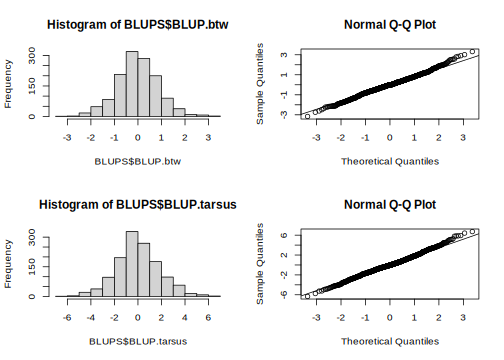
\includegraphics{wam_tuto_files/figure-latex/unnamed-chunk-85-1.pdf}

\begin{Shaded}
\begin{Highlighting}[]
\CommentTok{\#}
\KeywordTok{plot}\NormalTok{(BLUP.tarsus}\OperatorTok{\textasciitilde{}}\NormalTok{BLUP.btw,BLUPS,}\DataTypeTok{xlab=}\StringTok{""}\NormalTok{,}\DataTypeTok{ylab=}\StringTok{""}\NormalTok{, }\DataTypeTok{las=}\FloatTok{1.2}\NormalTok{, }\DataTypeTok{bty=}\StringTok{"o"}\NormalTok{, }\DataTypeTok{col=}\StringTok{"white"}\NormalTok{)}
\KeywordTok{arrows}\NormalTok{(}\DataTypeTok{x0=}\NormalTok{BLUPS}\OperatorTok{$}\NormalTok{BLUP.btw,}\DataTypeTok{y0=}\NormalTok{BLUPS}\OperatorTok{$}\NormalTok{BLUP.tarsus}\OperatorTok{{-}}\NormalTok{BLUPS}\OperatorTok{$}\NormalTok{SE.tarsus,}\DataTypeTok{x1=}\NormalTok{BLUPS}\OperatorTok{$}\NormalTok{BLUP.btw,}\DataTypeTok{y1=}\NormalTok{BLUPS}\OperatorTok{$}\NormalTok{BLUP.tarsus}\OperatorTok{+}\NormalTok{BLUPS}\OperatorTok{$}\NormalTok{SE.tarsus,}\DataTypeTok{col=}\StringTok{"black"}\NormalTok{,}\DataTypeTok{code=}\DecValTok{3}\NormalTok{,}\DataTypeTok{angle=}\DecValTok{90}\NormalTok{,}\DataTypeTok{length=}\DecValTok{0}\NormalTok{)}
\KeywordTok{arrows}\NormalTok{(}\DataTypeTok{x0=}\NormalTok{BLUPS}\OperatorTok{$}\NormalTok{BLUP.btw}\OperatorTok{{-}}\NormalTok{BLUPS}\OperatorTok{$}\NormalTok{SE.btw,}\DataTypeTok{y0=}\NormalTok{BLUPS}\OperatorTok{$}\NormalTok{BLUP.tarsus,}\DataTypeTok{x1=}\NormalTok{BLUPS}\OperatorTok{$}\NormalTok{BLUP.btw}\OperatorTok{+}\NormalTok{BLUPS}\OperatorTok{$}\NormalTok{SE.btw,}\DataTypeTok{y1=}\NormalTok{BLUPS}\OperatorTok{$}\NormalTok{BLUP.tarsus,}\DataTypeTok{col=}\StringTok{"black"}\NormalTok{,}\DataTypeTok{code=}\DecValTok{3}\NormalTok{,}\DataTypeTok{angle=}\DecValTok{90}\NormalTok{,}\DataTypeTok{length=}\DecValTok{0}\NormalTok{)}
\KeywordTok{points}\NormalTok{(BLUP.tarsus}\OperatorTok{\textasciitilde{}}\NormalTok{BLUP.btw,BLUPS,}\DataTypeTok{pch=}\DecValTok{16}\NormalTok{,}\DataTypeTok{col=}\StringTok{"red"}\NormalTok{, }\DataTypeTok{cex=}\FloatTok{1.5}\NormalTok{)}
\KeywordTok{points}\NormalTok{(BLUP.tarsus}\OperatorTok{\textasciitilde{}}\NormalTok{BLUP.btw,BLUPS,}\DataTypeTok{pch=}\DecValTok{1}\NormalTok{, }\DataTypeTok{col=}\KeywordTok{rgb}\NormalTok{(}\DecValTok{0}\NormalTok{,}\DecValTok{0}\NormalTok{,}\DecValTok{0}\NormalTok{,}\FloatTok{0.3}\NormalTok{), }\DataTypeTok{cex=}\KeywordTok{c}\NormalTok{(}\FloatTok{1.5}\NormalTok{))}
\KeywordTok{mtext}\NormalTok{(}\StringTok{"btw (BV±SE)"}\NormalTok{,  }\DataTypeTok{side=}\DecValTok{1}\NormalTok{, }\DataTypeTok{line=}\FloatTok{2.4}\NormalTok{)}
\KeywordTok{mtext}\NormalTok{(}\StringTok{"tarsus (BV±SE)"}\NormalTok{,  }\DataTypeTok{side=}\DecValTok{2}\NormalTok{, }\DataTypeTok{line=}\DecValTok{2}\NormalTok{,}\DataTypeTok{las=}\DecValTok{3}\NormalTok{)}
\KeywordTok{mtext}\NormalTok{(}\KeywordTok{expression}\NormalTok{(}\KeywordTok{paste}\NormalTok{(}\KeywordTok{italic}\NormalTok{(r)[A],}\StringTok{" = 0.7353065 ±  0.1094838"}\NormalTok{)),}\DataTypeTok{side=}\DecValTok{1}\NormalTok{,}\DataTypeTok{line=}\OperatorTok{{-}}\DecValTok{1}\NormalTok{,}\DataTypeTok{adj=}\FloatTok{0.95}\NormalTok{,}\DataTypeTok{cex=}\FloatTok{0.9}\NormalTok{)}
\end{Highlighting}
\end{Shaded}

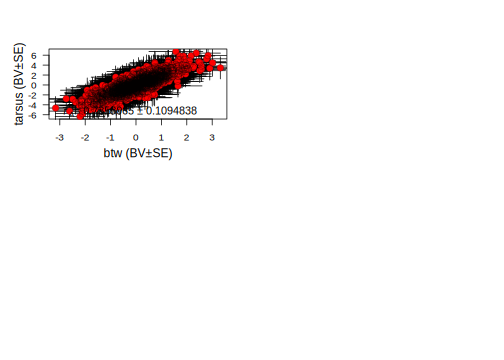
\includegraphics{wam_tuto_files/figure-latex/unnamed-chunk-85-2.pdf}

\hypertarget{partitionning-covariance-between-groups}{%
\subsection{Partitionning (co)variance between groups}\label{partitionning-covariance-between-groups}}

Similar to the univariate model, it is possible to partition the variance and also the covariance between different groups within the dataset. Here, we can estimate sex-specific genetic correlation.
Note, to partition a correlation, it is require to have important sample size within each group. For this example, we simplify the model !

\begin{Shaded}
\begin{Highlighting}[]
\NormalTok{gryphon \textless{}{-}}\StringTok{ }\NormalTok{gryphon[}\KeywordTok{order}\NormalTok{(gryphon}\OperatorTok{$}\NormalTok{sex), ]}
\NormalTok{model\_sex \textless{}{-}}\StringTok{ }\KeywordTok{asreml}\NormalTok{(}
  \DataTypeTok{fixed =} \KeywordTok{cbind}\NormalTok{(bwt, tarsus) }\OperatorTok{\textasciitilde{}}\StringTok{ }\NormalTok{trait }\OperatorTok{+}\StringTok{ }\KeywordTok{at}\NormalTok{(trait)}\OperatorTok{:}\NormalTok{sex,}
  \DataTypeTok{random =} \OperatorTok{\textasciitilde{}}\StringTok{ }\KeywordTok{at}\NormalTok{(sex)}\OperatorTok{:}\KeywordTok{us}\NormalTok{(trait)}\OperatorTok{:}\KeywordTok{vm}\NormalTok{(animal, ainv) }\OperatorTok{+}
\StringTok{    }\KeywordTok{us}\NormalTok{(trait, }\DataTypeTok{init =} \KeywordTok{c}\NormalTok{(}\DecValTok{1}\NormalTok{, }\FloatTok{0.1}\NormalTok{, }\DecValTok{1}\NormalTok{))}\OperatorTok{:}\NormalTok{byear }\OperatorTok{+}
\StringTok{    }\KeywordTok{us}\NormalTok{(trait, }\DataTypeTok{init =} \KeywordTok{c}\NormalTok{(}\DecValTok{1}\NormalTok{, }\FloatTok{0.1}\NormalTok{, }\DecValTok{1}\NormalTok{))}\OperatorTok{:}\NormalTok{mother,}
  \DataTypeTok{residual =} \OperatorTok{\textasciitilde{}}\StringTok{ }\KeywordTok{dsum}\NormalTok{(}\OperatorTok{\textasciitilde{}}\StringTok{ }\KeywordTok{id}\NormalTok{(units)}\OperatorTok{:}\KeywordTok{us}\NormalTok{(trait) }\OperatorTok{|}\StringTok{ }\NormalTok{sex),}
  \DataTypeTok{data =}\NormalTok{ gryphon,}
  \DataTypeTok{na.action =} \KeywordTok{na.method}\NormalTok{(}\DataTypeTok{x =} \StringTok{"include"}\NormalTok{, }\DataTypeTok{y =} \StringTok{"include"}\NormalTok{),}
  \DataTypeTok{maxit =} \DecValTok{20}
\NormalTok{)}
\end{Highlighting}
\end{Shaded}

\begin{verbatim}
## Warning in type.convert.default(x): 'as.is' should be specified by the caller;
## using TRUE

## Warning in type.convert.default(x): 'as.is' should be specified by the caller;
## using TRUE

## Warning in type.convert.default(x): 'as.is' should be specified by the caller;
## using TRUE

## Warning in type.convert.default(x): 'as.is' should be specified by the caller;
## using TRUE

## Warning in type.convert.default(x): 'as.is' should be specified by the caller;
## using TRUE

## Warning in type.convert.default(x): 'as.is' should be specified by the caller;
## using TRUE

## Warning in type.convert.default(x): 'as.is' should be specified by the caller;
## using TRUE

## Warning in type.convert.default(x): 'as.is' should be specified by the caller;
## using TRUE
\end{verbatim}

\begin{verbatim}
## Multi-section model using the sigma parameterization.
## ASReml 4.1.0 Tue Nov 23 22:11:00 2021
##           LogLik        Sigma2     DF     wall    cpu
##  1     -2495.853           1.0   1807 22:11:01    0.1 (1 restrained)
##  2     -2444.497           1.0   1807 22:11:01    0.1
##  3     -2401.367           1.0   1807 22:11:01    0.1
##  4     -2390.943           1.0   1807 22:11:01    0.1
##  5     -2388.819           1.0   1807 22:11:01    0.1
##  6     -2388.738           1.0   1807 22:11:01    0.1
##  7     -2388.736           1.0   1807 22:11:01    0.1
\end{verbatim}

\begin{Shaded}
\begin{Highlighting}[]
\NormalTok{model\_sex \textless{}{-}}\StringTok{ }\KeywordTok{update}\NormalTok{(model\_sex)}
\end{Highlighting}
\end{Shaded}

\begin{verbatim}
## Warning in type.convert.default(x): 'as.is' should be specified by the caller;
## using TRUE

## Warning in type.convert.default(x): 'as.is' should be specified by the caller;
## using TRUE

## Warning in type.convert.default(x): 'as.is' should be specified by the caller;
## using TRUE

## Warning in type.convert.default(x): 'as.is' should be specified by the caller;
## using TRUE

## Warning in type.convert.default(x): 'as.is' should be specified by the caller;
## using TRUE

## Warning in type.convert.default(x): 'as.is' should be specified by the caller;
## using TRUE

## Warning in type.convert.default(x): 'as.is' should be specified by the caller;
## using TRUE

## Warning in type.convert.default(x): 'as.is' should be specified by the caller;
## using TRUE
\end{verbatim}

\begin{verbatim}
## Multi-section model using the sigma parameterization.
## ASReml 4.1.0 Tue Nov 23 22:11:01 2021
##           LogLik        Sigma2     DF     wall    cpu
##  1     -2388.736           1.0   1807 22:11:01    0.1
##  2     -2388.736           1.0   1807 22:11:02    0.1
\end{verbatim}

\begin{Shaded}
\begin{Highlighting}[]
\KeywordTok{summary}\NormalTok{(model\_sex)}\OperatorTok{$}\NormalTok{varcomp}
\end{Highlighting}
\end{Shaded}

\begin{verbatim}
##                                                        component std.error
## trait:byear!trait_bwt:bwt                              0.9858502 0.2863930
## trait:byear!trait_tarsus:bwt                           0.1525073 0.4334219
## trait:byear!trait_tarsus:tarsus                        3.9981750 1.2798231
## trait:mother!trait_bwt:bwt                             1.3312802 0.2484496
## trait:mother!trait_tarsus:bwt                         -1.6173911 0.4283985
## trait:mother!trait_tarsus:tarsus                       4.7543015 1.3546795
## at(sex, 1):trait:vm(animal, ainv)!trait_bwt:bwt        1.3402726 0.5670807
## at(sex, 1):trait:vm(animal, ainv)!trait_tarsus:bwt     2.3607838 1.1348534
## at(sex, 1):trait:vm(animal, ainv)!trait_tarsus:tarsus  6.0624925 3.1304679
## at(sex, 2):trait:vm(animal, ainv)!trait_bwt:bwt        1.8645331 0.8887843
## at(sex, 2):trait:vm(animal, ainv)!trait_tarsus:bwt     5.0952433 2.0683128
## at(sex, 2):trait:vm(animal, ainv)!trait_tarsus:tarsus 14.9762227 6.4472652
## sex_1!R                                                1.0000000        NA
## sex_1!trait_bwt:bwt                                    2.3079924 0.5015700
## sex_1!trait_tarsus:bwt                                 4.4288323 1.0376540
## sex_1!trait_tarsus:tarsus                             13.4858721 2.9285483
## sex_2!R                                                1.0000000        NA
## sex_2!trait_bwt:bwt                                    1.7957128 0.7549623
## sex_2!trait_tarsus:bwt                                 2.6342177 1.7685005
## sex_2!trait_tarsus:tarsus                              9.6101885 5.4914087
##                                                          z.ratio bound %ch
## trait:byear!trait_bwt:bwt                              3.4422982     P 0.0
## trait:byear!trait_tarsus:bwt                           0.3518681     P 0.0
## trait:byear!trait_tarsus:tarsus                        3.1240060     P 0.0
## trait:mother!trait_bwt:bwt                             5.3583516     P 0.0
## trait:mother!trait_tarsus:bwt                         -3.7754356     P 0.0
## trait:mother!trait_tarsus:tarsus                       3.5095396     P 0.0
## at(sex, 1):trait:vm(animal, ainv)!trait_bwt:bwt        2.3634603     P 0.0
## at(sex, 1):trait:vm(animal, ainv)!trait_tarsus:bwt     2.0802544     P 0.0
## at(sex, 1):trait:vm(animal, ainv)!trait_tarsus:tarsus  1.9366091     P 0.0
## at(sex, 2):trait:vm(animal, ainv)!trait_bwt:bwt        2.0978466     P 0.0
## at(sex, 2):trait:vm(animal, ainv)!trait_tarsus:bwt     2.4634781     P 0.0
## at(sex, 2):trait:vm(animal, ainv)!trait_tarsus:tarsus  2.3228799     P 0.0
## sex_1!R                                                       NA     F 0.0
## sex_1!trait_bwt:bwt                                    4.6015360     P 0.0
## sex_1!trait_tarsus:bwt                                 4.2681204     P 0.0
## sex_1!trait_tarsus:tarsus                              4.6049683     P 0.0
## sex_2!R                                                       NA     F 0.0
## sex_2!trait_bwt:bwt                                    2.3785463     P 0.0
## sex_2!trait_tarsus:bwt                                 1.4895205     P 0.1
## sex_2!trait_tarsus:tarsus                              1.7500407     P 0.1
\end{verbatim}

we can estimate the different correlations using \texttt{vpredict}:

\begin{Shaded}
\begin{Highlighting}[]
\KeywordTok{vpredict}\NormalTok{(model\_sex, r\_byear }\OperatorTok{\textasciitilde{}}\StringTok{ }\NormalTok{V2 }\OperatorTok{/}\StringTok{ }\KeywordTok{sqrt}\NormalTok{(V1 }\OperatorTok{*}\StringTok{ }\NormalTok{V3))}
\end{Highlighting}
\end{Shaded}

\begin{verbatim}
##           Estimate       SE
## r_byear 0.07681647 0.213139
\end{verbatim}

\begin{Shaded}
\begin{Highlighting}[]
\KeywordTok{vpredict}\NormalTok{(model\_sex, r\_M }\OperatorTok{\textasciitilde{}}\StringTok{ }\NormalTok{V5 }\OperatorTok{/}\StringTok{ }\KeywordTok{sqrt}\NormalTok{(V4 }\OperatorTok{*}\StringTok{ }\NormalTok{V6))}
\end{Highlighting}
\end{Shaded}

\begin{verbatim}
##       Estimate        SE
## r_M -0.6428904 0.2489498
\end{verbatim}

\begin{Shaded}
\begin{Highlighting}[]
\KeywordTok{vpredict}\NormalTok{(model\_sex, r\_A}\FloatTok{.1} \OperatorTok{\textasciitilde{}}\StringTok{ }\NormalTok{V8 }\OperatorTok{/}\StringTok{ }\KeywordTok{sqrt}\NormalTok{(V7 }\OperatorTok{*}\StringTok{ }\NormalTok{V9))}
\end{Highlighting}
\end{Shaded}

\begin{verbatim}
##        Estimate        SE
## r_A.1 0.8281977 0.1723661
\end{verbatim}

\begin{Shaded}
\begin{Highlighting}[]
\KeywordTok{vpredict}\NormalTok{(model\_sex, r\_A}\FloatTok{.2} \OperatorTok{\textasciitilde{}}\StringTok{ }\NormalTok{V11 }\OperatorTok{/}\StringTok{ }\KeywordTok{sqrt}\NormalTok{(V10 }\OperatorTok{*}\StringTok{ }\NormalTok{V12))}
\end{Highlighting}
\end{Shaded}

\begin{verbatim}
##        Estimate        SE
## r_A.2 0.9642258 0.1241699
\end{verbatim}

\begin{Shaded}
\begin{Highlighting}[]
\KeywordTok{vpredict}\NormalTok{(model\_sex, r\_res}\FloatTok{.1} \OperatorTok{\textasciitilde{}}\StringTok{ }\NormalTok{V15 }\OperatorTok{/}\StringTok{ }\KeywordTok{sqrt}\NormalTok{(V14 }\OperatorTok{*}\StringTok{ }\NormalTok{V16))}
\end{Highlighting}
\end{Shaded}

\begin{verbatim}
##          Estimate        SE
## r_res.1 0.7938392 0.0789263
\end{verbatim}

\begin{Shaded}
\begin{Highlighting}[]
\KeywordTok{vpredict}\NormalTok{(model\_sex, r\_res}\FloatTok{.2} \OperatorTok{\textasciitilde{}}\StringTok{ }\NormalTok{V19 }\OperatorTok{/}\StringTok{ }\KeywordTok{sqrt}\NormalTok{(V18 }\OperatorTok{*}\StringTok{ }\NormalTok{V20))}
\end{Highlighting}
\end{Shaded}

\begin{verbatim}
##          Estimate        SE
## r_res.2 0.6341139 0.1894661
\end{verbatim}

and the heritability too:

\begin{Shaded}
\begin{Highlighting}[]
\KeywordTok{vpredict}\NormalTok{(model\_sex, h2.bwt}\FloatTok{.1} \OperatorTok{\textasciitilde{}}\StringTok{ }\NormalTok{V7 }\OperatorTok{/}\StringTok{ }\NormalTok{(V1 }\OperatorTok{+}\StringTok{ }\NormalTok{V4 }\OperatorTok{+}\StringTok{ }\NormalTok{V7 }\OperatorTok{+}\StringTok{ }\NormalTok{V14))}
\end{Highlighting}
\end{Shaded}

\begin{verbatim}
##           Estimate         SE
## h2.bwt.1 0.2246746 0.09176899
\end{verbatim}

\begin{Shaded}
\begin{Highlighting}[]
\KeywordTok{vpredict}\NormalTok{(model\_sex, h2.bwt}\FloatTok{.2} \OperatorTok{\textasciitilde{}}\StringTok{ }\NormalTok{V10 }\OperatorTok{/}\StringTok{ }\NormalTok{(V1 }\OperatorTok{+}\StringTok{ }\NormalTok{V4 }\OperatorTok{+}\StringTok{ }\NormalTok{V10 }\OperatorTok{+}\StringTok{ }\NormalTok{V18))}
\end{Highlighting}
\end{Shaded}

\begin{verbatim}
##           Estimate        SE
## h2.bwt.2 0.3119317 0.1442501
\end{verbatim}

\begin{Shaded}
\begin{Highlighting}[]
\KeywordTok{vpredict}\NormalTok{(model\_sex, h2.tarsus}\FloatTok{.1} \OperatorTok{\textasciitilde{}}\StringTok{ }\NormalTok{V9 }\OperatorTok{/}\StringTok{ }\NormalTok{(V3 }\OperatorTok{+}\StringTok{ }\NormalTok{V6 }\OperatorTok{+}\StringTok{ }\NormalTok{V9 }\OperatorTok{+}\StringTok{ }\NormalTok{V16))}
\end{Highlighting}
\end{Shaded}

\begin{verbatim}
##             Estimate        SE
## h2.tarsus.1 0.214216 0.1070477
\end{verbatim}

\begin{Shaded}
\begin{Highlighting}[]
\KeywordTok{vpredict}\NormalTok{(model\_sex, h2.tarsus}\FloatTok{.2} \OperatorTok{\textasciitilde{}}\StringTok{ }\NormalTok{V12 }\OperatorTok{/}\StringTok{ }\NormalTok{(V3 }\OperatorTok{+}\StringTok{ }\NormalTok{V6 }\OperatorTok{+}\StringTok{ }\NormalTok{V12 }\OperatorTok{+}\StringTok{ }\NormalTok{V20))}
\end{Highlighting}
\end{Shaded}

\begin{verbatim}
##              Estimate        SE
## h2.tarsus.2 0.4492118 0.1833703
\end{verbatim}

Now we can look at the fixed effects parameters and assess their significance with a conditional Wald F-test:

\begin{Shaded}
\begin{Highlighting}[]
\KeywordTok{summary}\NormalTok{(model\_sex, }\DataTypeTok{coef =} \OtherTok{TRUE}\NormalTok{)}\OperatorTok{$}\NormalTok{coef.fi}
\KeywordTok{wald.asreml}\NormalTok{(model\_sex, }\DataTypeTok{denDF =} \StringTok{"default"}\NormalTok{, }\DataTypeTok{ssType =} \StringTok{"conditional"}\NormalTok{)}\OperatorTok{$}\NormalTok{Wald}
\end{Highlighting}
\end{Shaded}

\begin{verbatim}
##                            solution std error    z.ratio
## at(trait, tarsus):sex_1  0.00000000        NA         NA
## at(trait, tarsus):sex_2 -0.05549717 0.4758546 -0.1166263
## at(trait, bwt):sex_1     0.00000000        NA         NA
## at(trait, bwt):sex_2     1.93936200 0.1903213 10.1899393
## trait_bwt                6.37791872 0.2311775 27.5888427
## trait_tarsus            20.58389296 0.4942600 41.6458836
\end{verbatim}

\begin{verbatim}
## Warning in type.convert.default(x): 'as.is' should be specified by the caller;
## using TRUE

## Warning in type.convert.default(x): 'as.is' should be specified by the caller;
## using TRUE

## Warning in type.convert.default(x): 'as.is' should be specified by the caller;
## using TRUE

## Warning in type.convert.default(x): 'as.is' should be specified by the caller;
## using TRUE

## Warning in type.convert.default(x): 'as.is' should be specified by the caller;
## using TRUE

## Warning in type.convert.default(x): 'as.is' should be specified by the caller;
## using TRUE

## Warning in type.convert.default(x): 'as.is' should be specified by the caller;
## using TRUE

## Warning in type.convert.default(x): 'as.is' should be specified by the caller;
## using TRUE
\end{verbatim}

\begin{verbatim}
## Multi-section model using the sigma parameterization.
## ASReml 4.1.0 Tue Nov 23 22:11:02 2021
##           LogLik        Sigma2     DF     wall    cpu
##  1     -2388.736           1.0   1807 22:11:02    0.1
##  2     -2388.736           1.0   1807 22:11:02    0.1
## Calculating denominator DF
\end{verbatim}

\begin{verbatim}
## 
##                       Df denDF   F.inc   F.con Margin      Pr
## trait                  2  44.8 1522.00 1522.00        0.00000
## at(trait, bwt):sex     1 137.5  220.90  103.80      B 0.00000
## at(trait, tarsus):sex  1 138.6    0.01    0.01      B 0.90737
\end{verbatim}

\hypertarget{gremlin-2}{%
\section{gremlin}\label{gremlin-2}}

Might not available yet
Meanwhile

\begin{figure}

\includegraphics[width=1\linewidth]{images/Gizmo} \caption{Keep it dry and do no feed after midnight.}\label{fig:unnamed-chunk-91}
\end{figure}

\hypertarget{mcmcglmm-2}{%
\section{MCMCglmm}\label{mcmcglmm-2}}

\texttt{MCMCglmm} has the advantage to keep automatically keep the lines with missing data and will try to fit the model use latent variables for missing data.
For comparison, we will remove the missing values from the data before fitting the model.

\begin{Shaded}
\begin{Highlighting}[]
\NormalTok{gryphon2 \textless{}{-}}\StringTok{ }\KeywordTok{subset}\NormalTok{(gryphon, }\OperatorTok{!}\KeywordTok{is.na}\NormalTok{(bwt) }\OperatorTok{\&}\StringTok{ }\OperatorTok{!}\KeywordTok{is.na}\NormalTok{(tarsus))}
\end{Highlighting}
\end{Shaded}

First load MCMCglmm:

\begin{Shaded}
\begin{Highlighting}[]
\KeywordTok{library}\NormalTok{(MCMCglmm)}
\NormalTok{Ainv \textless{}{-}}\StringTok{ }\KeywordTok{inverseA}\NormalTok{(gryphonped)}\OperatorTok{$}\NormalTok{Ainv}
\end{Highlighting}
\end{Shaded}

\hypertarget{fitting-the-model}{%
\subsection{Fitting the model}\label{fitting-the-model}}

Fitting a multivariate model in MCMCglmm involves several new consideration above those for fitting univariate models. First, we have to fit multivariate priors; second, we have to specify the ways in which effects on different traits may covary, including the nature of residual (co)variation; and third, we will have to be a little more specific when specifying to MCMCglmm what type of distributions from which we assume our data are drawn. Our most basic model can be specified as:

\begin{Shaded}
\begin{Highlighting}[]
\NormalTok{prior2}\FloatTok{.1}\NormalTok{ \textless{}{-}}\StringTok{ }\KeywordTok{list}\NormalTok{(}
  \DataTypeTok{G =} \KeywordTok{list}\NormalTok{(}\DataTypeTok{G1 =} \KeywordTok{list}\NormalTok{(}\DataTypeTok{V =} \KeywordTok{diag}\NormalTok{(}\DecValTok{2}\NormalTok{), }\DataTypeTok{nu =} \FloatTok{1.002}\NormalTok{)),}
  \DataTypeTok{R =} \KeywordTok{list}\NormalTok{(}\DataTypeTok{V =} \KeywordTok{diag}\NormalTok{(}\DecValTok{2}\NormalTok{), }\DataTypeTok{nu =} \FloatTok{1.002}\NormalTok{)}
\NormalTok{)}

\NormalTok{model2}\FloatTok{.1}\NormalTok{ \textless{}{-}}\StringTok{ }\KeywordTok{MCMCglmm}\NormalTok{(}\KeywordTok{cbind}\NormalTok{(bwt, tarsus) }\OperatorTok{\textasciitilde{}}\StringTok{ }\NormalTok{trait }\OperatorTok{{-}}\StringTok{ }\DecValTok{1}\NormalTok{,}
  \DataTypeTok{random =} \OperatorTok{\textasciitilde{}}\StringTok{ }\KeywordTok{us}\NormalTok{(trait)}\OperatorTok{:}\NormalTok{animal,}
  \DataTypeTok{rcov =} \OperatorTok{\textasciitilde{}}\StringTok{ }\KeywordTok{us}\NormalTok{(trait)}\OperatorTok{:}\NormalTok{units,}
  \DataTypeTok{family =} \KeywordTok{c}\NormalTok{(}\StringTok{"gaussian"}\NormalTok{, }\StringTok{"gaussian"}\NormalTok{),}
  \DataTypeTok{ginv =} \KeywordTok{list}\NormalTok{(}\DataTypeTok{animal =}\NormalTok{ Ainv),}
  \DataTypeTok{data =}\NormalTok{ gryphon, }\DataTypeTok{prior =}\NormalTok{ prior2}\FloatTok{.1}\NormalTok{, }\DataTypeTok{verbose =} \OtherTok{FALSE}
\NormalTok{)}
\KeywordTok{summary}\NormalTok{(model2}\FloatTok{.1}\NormalTok{)}
\end{Highlighting}
\end{Shaded}

\begin{verbatim}
## 
##  Iterations = 3001:12991
##  Thinning interval  = 10
##  Sample size  = 1000 
## 
##  DIC: 7924.734 
## 
##  G-structure:  ~us(trait):animal
## 
##                                post.mean l-95% CI u-95% CI eff.samp
## traitbwt:traitbwt.animal           3.351   2.2344    4.555   167.36
## traittarsus:traitbwt.animal        2.322   0.1981    4.319    98.01
## traitbwt:traittarsus.animal        2.322   0.1981    4.319    98.01
## traittarsus:traittarsus.animal    11.631   4.8169   18.703    59.15
## 
##  R-structure:  ~us(trait):units
## 
##                               post.mean l-95% CI u-95% CI eff.samp
## traitbwt:traitbwt.units           3.905    2.969    4.928   172.53
## traittarsus:traitbwt.units        3.467    1.870    5.545   143.33
## traitbwt:traittarsus.units        3.467    1.870    5.545   143.33
## traittarsus:traittarsus.units    18.485   13.070   24.898    73.11
## 
##  Location effects: cbind(bwt, tarsus) ~ trait - 1 
## 
##             post.mean l-95% CI u-95% CI eff.samp  pMCMC    
## traitbwt        7.586    7.332    7.876    847.3 <0.001 ***
## traittarsus    20.522   20.024   21.157    776.4 <0.001 ***
## ---
## Signif. codes:  0 '***' 0.001 '**' 0.01 '*' 0.05 '.' 0.1 ' ' 1
\end{verbatim}

\begin{Shaded}
\begin{Highlighting}[]
\KeywordTok{plot}\NormalTok{(model2}\FloatTok{.1}\OperatorTok{$}\NormalTok{VCV[, }\StringTok{"traittarsus:traittarsus.animal"}\NormalTok{])}
\end{Highlighting}
\end{Shaded}

\begin{figure}
\centering
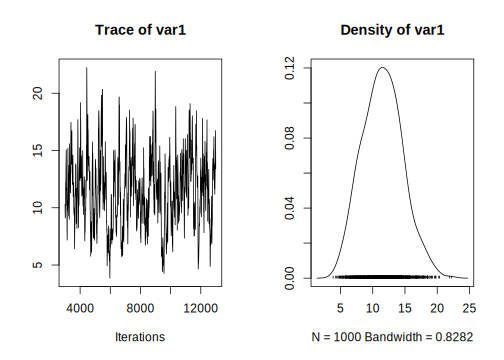
\includegraphics{wam_tuto_files/figure-latex/unnamed-chunk-94-1.pdf}
\caption{\label{fig:unnamed-chunk-94}The posterior distribution of the additive genetic effect for tarsus length in a MCMCglmm run with default values}
\end{figure}

\begin{Shaded}
\begin{Highlighting}[]
\KeywordTok{autocorr.diag}\NormalTok{(model2}\FloatTok{.1}\OperatorTok{$}\NormalTok{VCV)[, }\StringTok{"traittarsus:traittarsus.animal"}\NormalTok{][}\DecValTok{2}\NormalTok{]}
\end{Highlighting}
\end{Shaded}

\begin{verbatim}
##    Lag 10 
## 0.8512688
\end{verbatim}

We have constructed the prior similarly to the those in the univariate models in tutorial 1, only we are specifying a 2x2 covariance matrix rather than a single variance. In order to provide proper priors, we have set the degree of belief parameter to greater than 1 (1.002). Those priors are not necessarily weak or uninformative in all circumstances. We will consider them adequate nonetheless for this tutorial. Please the vignette of the MCMCglmm packages \citep{R-MCMCglmm} for more information on priors. In tutorial 1, we used full autocorrelation tables to evaluate the validity of the posterior distribution. Note that we have not done this here.
For a bivariate model this table can become very complex. Nonetheless, it is worth evaluating, rather it is simply to large to include here. It can be viewed in the console as before. Here we have displayed only the autocorrelation for estimates of additive genetic effects for tarsus length with a lag of one samples (10 iterations given this MCMCglmm run with default values). This lag of 0.8512688 is clearly unacceptable. The posterior distribution of the additive genetic effect on tarsus length is shown in Figure 4 (p.~15), note the autocorrelation evident in the left-hand plot.

We will opt to run the analysis for longer. This longer run could be run using the following code (including a line to save the output):

\begin{Shaded}
\begin{Highlighting}[]
\NormalTok{model2}\FloatTok{.1}\NormalTok{ \textless{}{-}}\StringTok{ }\KeywordTok{MCMCglmm}\NormalTok{(}\KeywordTok{cbind}\NormalTok{(bwt, tarsus) }\OperatorTok{\textasciitilde{}}\StringTok{ }\NormalTok{trait }\OperatorTok{{-}}\StringTok{ }\DecValTok{1}\NormalTok{,}
  \DataTypeTok{random =} \OperatorTok{\textasciitilde{}}\StringTok{ }\KeywordTok{us}\NormalTok{(trait)}\OperatorTok{:}\NormalTok{animal,}
  \DataTypeTok{rcov =} \OperatorTok{\textasciitilde{}}\StringTok{ }\KeywordTok{us}\NormalTok{(trait)}\OperatorTok{:}\NormalTok{units,}
  \DataTypeTok{family =} \KeywordTok{c}\NormalTok{(}\StringTok{"gaussian"}\NormalTok{, }\StringTok{"gaussian"}\NormalTok{),}
  \DataTypeTok{ginv =} \KeywordTok{list}\NormalTok{(}\DataTypeTok{animal =}\NormalTok{ Ainv),}
  \DataTypeTok{data =}\NormalTok{ gryphon,}
  \DataTypeTok{nitt =} \DecValTok{130000}\NormalTok{, }\DataTypeTok{thin =} \DecValTok{100}\NormalTok{, }\DataTypeTok{burnin =} \DecValTok{30000}\NormalTok{,}
  \DataTypeTok{prior =}\NormalTok{ prior2}\FloatTok{.1}\NormalTok{, }\DataTypeTok{verbose =} \OtherTok{FALSE}
\NormalTok{)}
\KeywordTok{save}\NormalTok{(model2}\FloatTok{.1}\NormalTok{, }\DataTypeTok{file =} \StringTok{"data/MCMCglmm\_model2\_1\_LongRun.rda"}\NormalTok{)}
\end{Highlighting}
\end{Shaded}

However, this run might take as long as an hour. For the purpose of this tutorial we have provided an output for such a run. It can be obtained and manipulated as follows, assuming that the file \texttt{MCMCglmm\_model2\_1\_LongRun.rda} is available at the specified location:

\begin{Shaded}
\begin{Highlighting}[]
\KeywordTok{load}\NormalTok{(}\DataTypeTok{file =} \StringTok{"data/MCMCglmm\_model2\_1\_LongRun.rda"}\NormalTok{)}
\KeywordTok{autocorr.diag}\NormalTok{(model2}\FloatTok{.1}\OperatorTok{$}\NormalTok{VCV)[, }\StringTok{"traittarsus:traittarsus.animal"}\NormalTok{][}\DecValTok{2}\NormalTok{]}
\end{Highlighting}
\end{Shaded}

\begin{verbatim}
##   Lag 100 
## 0.2608752
\end{verbatim}

This level of autocorrelation is more acceptable, at least for the purpose of demonstration in this tutorial.
We can recover variance components, heritabilities, and genetic correlations from the posterior distribution of this model:

\begin{Shaded}
\begin{Highlighting}[]
\KeywordTok{posterior.mode}\NormalTok{(model2}\FloatTok{.1}\OperatorTok{$}\NormalTok{VCV)}
\end{Highlighting}
\end{Shaded}

\begin{verbatim}
##       traitbwt:traitbwt.animal    traittarsus:traitbwt.animal 
##                       3.370616                       2.581839 
##    traitbwt:traittarsus.animal traittarsus:traittarsus.animal 
##                       2.581839                      12.463915 
##        traitbwt:traitbwt.units     traittarsus:traitbwt.units 
##                       3.761401                       2.982413 
##     traitbwt:traittarsus.units  traittarsus:traittarsus.units 
##                       2.982413                      19.556443
\end{verbatim}

\begin{Shaded}
\begin{Highlighting}[]
\NormalTok{heritability.bwt2}\FloatTok{.1}\NormalTok{ \textless{}{-}}\StringTok{ }\NormalTok{model2}\FloatTok{.1}\OperatorTok{$}\NormalTok{VCV[, }\StringTok{"traitbwt:traitbwt.animal"}\NormalTok{] }\OperatorTok{/}\StringTok{ }\NormalTok{(model2}\FloatTok{.1}\OperatorTok{$}\NormalTok{VCV[, }\StringTok{"traitbwt:traitbwt.animal"}\NormalTok{] }\OperatorTok{+}\StringTok{ }\NormalTok{model2}\FloatTok{.1}\OperatorTok{$}\NormalTok{VCV[, }\StringTok{"traitbwt:traitbwt.animal"}\NormalTok{])}
\KeywordTok{posterior.mode}\NormalTok{(heritability.bwt2}\FloatTok{.1}\NormalTok{)}
\end{Highlighting}
\end{Shaded}

\begin{verbatim}
##      var1 
## 0.4999336
\end{verbatim}

\begin{Shaded}
\begin{Highlighting}[]
\NormalTok{heritability.tarsus2}\FloatTok{.1}\NormalTok{ \textless{}{-}}\StringTok{ }\NormalTok{model2}\FloatTok{.1}\OperatorTok{$}\NormalTok{VCV[, }\StringTok{"traittarsus:traittarsus.animal"}\NormalTok{] }\OperatorTok{/}\StringTok{ }\NormalTok{(model2}\FloatTok{.1}\OperatorTok{$}\NormalTok{VCV[, }\StringTok{"traittarsus:traittarsus.animal"}\NormalTok{] }\OperatorTok{+}\StringTok{ }\NormalTok{model2}\FloatTok{.1}\OperatorTok{$}\NormalTok{VCV[, }\StringTok{"traittarsus:traittarsus.units"}\NormalTok{])}
\KeywordTok{posterior.mode}\NormalTok{(heritability.tarsus2}\FloatTok{.1}\NormalTok{)}
\end{Highlighting}
\end{Shaded}

\begin{verbatim}
##      var1 
## 0.4038754
\end{verbatim}

\begin{Shaded}
\begin{Highlighting}[]
\NormalTok{genetic.correlation2}\FloatTok{.1}\NormalTok{ \textless{}{-}}\StringTok{ }\NormalTok{model2}\FloatTok{.1}\OperatorTok{$}\NormalTok{VCV[, }\StringTok{"traitbwt:traittarsus.animal"}\NormalTok{] }\OperatorTok{/}\StringTok{ }\KeywordTok{sqrt}\NormalTok{(model2}\FloatTok{.1}\OperatorTok{$}\NormalTok{VCV[, }\StringTok{"traitbwt:traitbwt.animal"}\NormalTok{] }\OperatorTok{*}\StringTok{ }\NormalTok{model2}\FloatTok{.1}\OperatorTok{$}\NormalTok{VCV[, }\StringTok{"traittarsus:traittarsus.animal"}\NormalTok{])}
\KeywordTok{posterior.mode}\NormalTok{(genetic.correlation2}\FloatTok{.1}\NormalTok{)}
\end{Highlighting}
\end{Shaded}

\begin{verbatim}
##      var1 
## 0.3691503
\end{verbatim}

\hypertarget{adding-fixed-and-random-effects-1}{%
\subsection{Adding fixed and random effects}\label{adding-fixed-and-random-effects-1}}

Fixed and random effects can be added just as for the univariate case.
Given that our full model of bwt from tutorial 1 had sex as a fixed effect as well as random effects of byear and mother, we could specify a bivariate formulation of this using the following code (including a line to save the output):

\begin{Shaded}
\begin{Highlighting}[]
\NormalTok{prior2}\FloatTok{.2}\NormalTok{ \textless{}{-}}\StringTok{ }\KeywordTok{list}\NormalTok{(}
  \DataTypeTok{G =} \KeywordTok{list}\NormalTok{(}
    \DataTypeTok{G1 =} \KeywordTok{list}\NormalTok{(}\DataTypeTok{V =} \KeywordTok{diag}\NormalTok{(}\DecValTok{2}\NormalTok{), }\DataTypeTok{nu =} \FloatTok{1.002}\NormalTok{),}
    \DataTypeTok{G2 =} \KeywordTok{list}\NormalTok{(}\DataTypeTok{V =} \KeywordTok{diag}\NormalTok{(}\DecValTok{2}\NormalTok{), }\DataTypeTok{nu =} \FloatTok{1.002}\NormalTok{),}
    \DataTypeTok{G3 =} \KeywordTok{list}\NormalTok{(}\DataTypeTok{V =} \KeywordTok{diag}\NormalTok{(}\DecValTok{2}\NormalTok{), }\DataTypeTok{nu =} \FloatTok{1.002}\NormalTok{)}
\NormalTok{  ),}
  \DataTypeTok{R =} \KeywordTok{list}\NormalTok{(}\DataTypeTok{V =} \KeywordTok{diag}\NormalTok{(}\DecValTok{2}\NormalTok{), }\DataTypeTok{nu =} \FloatTok{1.002}\NormalTok{)}
\NormalTok{)}
\NormalTok{model2}\FloatTok{.2}\NormalTok{ \textless{}{-}}\StringTok{ }\KeywordTok{MCMCglmm}\NormalTok{(}\KeywordTok{cbind}\NormalTok{(bwt, tarsus) }\OperatorTok{\textasciitilde{}}\StringTok{ }\NormalTok{trait }\OperatorTok{{-}}\StringTok{ }\DecValTok{1} \OperatorTok{+}\StringTok{ }\NormalTok{trait}\OperatorTok{:}\NormalTok{sex,}
  \DataTypeTok{random =} \OperatorTok{\textasciitilde{}}\StringTok{ }\KeywordTok{us}\NormalTok{(trait)}\OperatorTok{:}\NormalTok{animal }\OperatorTok{+}\StringTok{ }\KeywordTok{us}\NormalTok{(trait)}\OperatorTok{:}\NormalTok{byear }\OperatorTok{+}\StringTok{ }\KeywordTok{us}\NormalTok{(trait)}\OperatorTok{:}\NormalTok{mother,}
  \DataTypeTok{rcov =} \OperatorTok{\textasciitilde{}}\StringTok{ }\KeywordTok{us}\NormalTok{(trait)}\OperatorTok{:}\NormalTok{units,}
  \DataTypeTok{family =} \KeywordTok{c}\NormalTok{(}\StringTok{"gaussian"}\NormalTok{, }\StringTok{"gaussian"}\NormalTok{),}
  \DataTypeTok{ginv =} \KeywordTok{list}\NormalTok{(}\DataTypeTok{animal =}\NormalTok{ Ainv), }\DataTypeTok{data =}\NormalTok{ gryphon,}
  \DataTypeTok{nitt =} \DecValTok{130000}\NormalTok{, }\DataTypeTok{thin =} \DecValTok{100}\NormalTok{, }\DataTypeTok{burnin =} \DecValTok{30000}\NormalTok{,}
  \DataTypeTok{prior =}\NormalTok{ prior2}\FloatTok{.2}\NormalTok{, }\DataTypeTok{verbose =} \OtherTok{FALSE}
\NormalTok{)}
\KeywordTok{save}\NormalTok{(model2}\FloatTok{.2}\NormalTok{, }\DataTypeTok{file =} \StringTok{"data/MCMCglmm\_model2\_2\_LongRun.rda"}\NormalTok{)}
\end{Highlighting}
\end{Shaded}

Again we have provided the data from one such run. It can be accessed using the code:

\begin{Shaded}
\begin{Highlighting}[]
\KeywordTok{load}\NormalTok{(}\DataTypeTok{file =} \StringTok{"data/MCMCglmm\_model2\_2\_LongRun.rda"}\NormalTok{)}
\KeywordTok{summary}\NormalTok{(model2}\FloatTok{.2}\NormalTok{)}
\end{Highlighting}
\end{Shaded}

\begin{verbatim}
## 
##  Iterations = 30001:529501
##  Thinning interval  = 500
##  Sample size  = 1000 
## 
##  DIC: 6222.288 
## 
##  G-structure:  ~us(trait):animal
## 
##                                post.mean  l-95% CI u-95% CI eff.samp
## traitbwt:traitbwt.animal           1.237  0.010802    2.183    71.22
## traittarsus:traitbwt.animal        2.138 -0.067106    4.268    49.85
## traitbwt:traittarsus.animal        2.138 -0.067106    4.268    49.85
## traittarsus:traittarsus.animal     5.265  0.005733   11.751    49.24
## 
##                ~us(trait):byear
## 
##                               post.mean l-95% CI u-95% CI eff.samp
## traitbwt:traitbwt.byear         0.85157   0.3924   1.3839     1000
## traittarsus:traitbwt.byear     -0.01322  -0.7624   0.8352     1000
## traitbwt:traittarsus.byear     -0.01322  -0.7624   0.8352     1000
## traittarsus:traittarsus.byear   3.30411   1.2574   5.6918     1000
## 
##                ~us(trait):mother
## 
##                                post.mean l-95% CI u-95% CI eff.samp
## traitbwt:traitbwt.mother           1.213   0.7414    1.688    164.7
## traittarsus:traitbwt.mother       -1.969  -2.3860   -1.533    422.4
## traitbwt:traittarsus.mother       -1.969  -2.3860   -1.533    422.4
## traittarsus:traittarsus.mother     3.484   1.7016    5.451    215.8
## 
##  R-structure:  ~us(trait):units
## 
##                               post.mean l-95% CI u-95% CI eff.samp
## traitbwt:traitbwt.units           2.531    1.618    3.485   133.27
## traittarsus:traitbwt.units        5.360    3.508    7.703    76.07
## traitbwt:traittarsus.units        5.360    3.508    7.703    76.07
## traittarsus:traittarsus.units    17.744   11.386   23.397    61.97
## 
##  Location effects: cbind(bwt, tarsus) ~ trait - 1 + trait:sex 
## 
##                  post.mean l-95% CI u-95% CI eff.samp  pMCMC    
## traitbwt            6.2643   5.8046   6.7063     1027 <0.001 ***
## traittarsus        20.3901  19.4377  21.2534     1000 <0.001 ***
## traitbwt:sex2       2.0315   1.7096   2.3452     1000 <0.001 ***
## traittarsus:sex2    0.1141  -0.6095   0.8959     1000  0.746    
## ---
## Signif. codes:  0 '***' 0.001 '**' 0.01 '*' 0.05 '.' 0.1 ' ' 1
\end{verbatim}

\begin{Shaded}
\begin{Highlighting}[]
\KeywordTok{autocorr}\NormalTok{(model2}\FloatTok{.2}\OperatorTok{$}\NormalTok{VCV)[, , }\StringTok{"traittarsus:traittarsus.animal"}\NormalTok{][}\DecValTok{3}\NormalTok{, }\DecValTok{4}\NormalTok{]}
\end{Highlighting}
\end{Shaded}

\begin{verbatim}
## [1] 0.5231926
\end{verbatim}

We can evaluate the fixed effect, their Ci evaluate their significance.

\begin{Shaded}
\begin{Highlighting}[]
\KeywordTok{posterior.mode}\NormalTok{(model2}\FloatTok{.2}\OperatorTok{$}\NormalTok{Sol)}
\end{Highlighting}
\end{Shaded}

\begin{verbatim}
##         traitbwt      traittarsus    traitbwt:sex2 traittarsus:sex2 
##       6.37708530      20.33434582       1.97881662       0.00709564
\end{verbatim}

\begin{Shaded}
\begin{Highlighting}[]
\KeywordTok{HPDinterval}\NormalTok{(model2}\FloatTok{.2}\OperatorTok{$}\NormalTok{Sol, }\FloatTok{0.95}\NormalTok{)}
\end{Highlighting}
\end{Shaded}

\begin{verbatim}
##                       lower     upper
## traitbwt          5.8045704  6.706339
## traittarsus      19.4377228 21.253397
## traitbwt:sex2     1.7095714  2.345200
## traittarsus:sex2 -0.6094733  0.895885
## attr(,"Probability")
## [1] 0.95
\end{verbatim}

\begin{Shaded}
\begin{Highlighting}[]
\KeywordTok{plot}\NormalTok{(model2}\FloatTok{.2}\OperatorTok{$}\NormalTok{Sol)}
\end{Highlighting}
\end{Shaded}

\begin{figure}
\centering
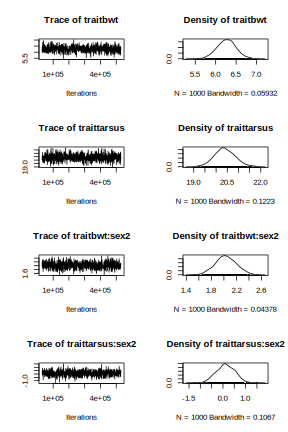
\includegraphics{wam_tuto_files/figure-latex/unnamed-chunk-100-1.pdf}
\caption{\label{fig:unnamed-chunk-100}Posterior trace and distribution for the fixed effects in model 2.2}
\end{figure}

As before we can obtain the raw variance component estimates and genetic correlations for the random effects:

\begin{Shaded}
\begin{Highlighting}[]
\KeywordTok{posterior.mode}\NormalTok{(model2}\FloatTok{.2}\OperatorTok{$}\NormalTok{VCV)}
\end{Highlighting}
\end{Shaded}

\begin{verbatim}
##       traitbwt:traitbwt.animal    traittarsus:traitbwt.animal 
##                     1.32761860                     1.98076467 
##    traitbwt:traittarsus.animal traittarsus:traittarsus.animal 
##                     1.98076467                     0.07827994 
##        traitbwt:traitbwt.byear     traittarsus:traitbwt.byear 
##                     0.83300490                    -0.14691430 
##     traitbwt:traittarsus.byear  traittarsus:traittarsus.byear 
##                    -0.14691430                     2.79242863 
##       traitbwt:traitbwt.mother    traittarsus:traitbwt.mother 
##                     1.29299116                    -1.97967150 
##    traitbwt:traittarsus.mother traittarsus:traittarsus.mother 
##                    -1.97967150                     3.71594577 
##        traitbwt:traitbwt.units     traittarsus:traitbwt.units 
##                     2.53632072                     5.22764927 
##     traitbwt:traittarsus.units  traittarsus:traittarsus.units 
##                     5.22764927                    16.57931045
\end{verbatim}

\begin{Shaded}
\begin{Highlighting}[]
\NormalTok{genetic.correlation2}\FloatTok{.2}\NormalTok{ \textless{}{-}}\StringTok{ }\NormalTok{model2}\FloatTok{.2}\OperatorTok{$}\NormalTok{VCV[, }\StringTok{"traitbwt:traittarsus.animal"}\NormalTok{] }\OperatorTok{/}\StringTok{ }\KeywordTok{sqrt}\NormalTok{(model2}\FloatTok{.2}\OperatorTok{$}\NormalTok{VCV[, }\StringTok{"traitbwt:traitbwt.animal"}\NormalTok{] }\OperatorTok{*}\StringTok{ }\NormalTok{model2}\FloatTok{.2}\OperatorTok{$}\NormalTok{VCV[, }\StringTok{"traittarsus:traittarsus.animal"}\NormalTok{])}
\NormalTok{maternal.correlation2}\FloatTok{.2}\NormalTok{ \textless{}{-}}\StringTok{ }\NormalTok{model2}\FloatTok{.2}\OperatorTok{$}\NormalTok{VCV[, }\StringTok{"traitbwt:traittarsus.mother"}\NormalTok{] }\OperatorTok{/}\StringTok{ }\KeywordTok{sqrt}\NormalTok{(model2}\FloatTok{.2}\OperatorTok{$}\NormalTok{VCV[, }\StringTok{"traitbwt:traitbwt.mother"}\NormalTok{] }\OperatorTok{*}\StringTok{ }\NormalTok{model2}\FloatTok{.2}\OperatorTok{$}\NormalTok{VCV[, }\StringTok{"traittarsus:traittarsus.mother"}\NormalTok{])}
\KeywordTok{posterior.mode}\NormalTok{(genetic.correlation2}\FloatTok{.2}\NormalTok{)}
\end{Highlighting}
\end{Shaded}

\begin{verbatim}
##      var1 
## 0.9942065
\end{verbatim}

\begin{Shaded}
\begin{Highlighting}[]
\KeywordTok{posterior.mode}\NormalTok{(maternal.correlation2}\FloatTok{.2}\NormalTok{)}
\end{Highlighting}
\end{Shaded}

\begin{verbatim}
##       var1 
## -0.9920879
\end{verbatim}

Evaluation of the statistical support for these genetic and maternal correlations is straightforward. Because we imposed no constraint on their estimation, we can evaluate the extent to which the posterior distributions overlap zero:

\begin{Shaded}
\begin{Highlighting}[]
\KeywordTok{HPDinterval}\NormalTok{(genetic.correlation2}\FloatTok{.2}\NormalTok{, }\FloatTok{0.95}\NormalTok{)}
\end{Highlighting}
\end{Shaded}

\begin{verbatim}
##          lower     upper
## var1 0.3935369 0.9990187
## attr(,"Probability")
## [1] 0.95
\end{verbatim}

\begin{Shaded}
\begin{Highlighting}[]
\KeywordTok{HPDinterval}\NormalTok{(maternal.correlation2}\FloatTok{.2}\NormalTok{, }\FloatTok{0.95}\NormalTok{)}
\end{Highlighting}
\end{Shaded}

\begin{verbatim}
##           lower      upper
## var1 -0.9980476 -0.9443838
## attr(,"Probability")
## [1] 0.95
\end{verbatim}

Neither or these posterior distributions overlaps zero, so we can consider them both statistically supported.

\hypertarget{direct-estimate-of-the-correlation-instead-of-the-covariance.}{%
\subsection{Direct estimate of the correlation instead of the covariance.}\label{direct-estimate-of-the-correlation-instead-of-the-covariance.}}

For this example, we just estimate the correlation at the geneticvel, the covariance for the other random effect (\texttt{mother} and \texttt{byear}) and the resdisual level was not estimate to help the model to converge and compute faster. The prior will be the same but we change the \texttt{pr} argument to be \texttt{TRUE} to keep the posterior distribution of random effects.
To simplify the following code, we rename the variable T1 and T2.

\begin{Shaded}
\begin{Highlighting}[]
\CommentTok{\#}
\NormalTok{gryphon}\OperatorTok{$}\NormalTok{T1\textless{}{-}gryphon}\OperatorTok{$}\NormalTok{bwt}
\NormalTok{gryphon}\OperatorTok{$}\NormalTok{T2\textless{}{-}gryphon}\OperatorTok{$}\NormalTok{tarsus}

\NormalTok{model2}\FloatTok{.3}\NormalTok{ \textless{}{-}}\StringTok{ }\KeywordTok{MCMCglmm}\NormalTok{(}\KeywordTok{cbind}\NormalTok{(T1, T2) }\OperatorTok{\textasciitilde{}}\StringTok{ }\NormalTok{trait }\OperatorTok{{-}}\StringTok{ }\DecValTok{1} \OperatorTok{+}\StringTok{ }\NormalTok{trait}\OperatorTok{:}\NormalTok{sex,}
  \DataTypeTok{random =} \OperatorTok{\textasciitilde{}}\StringTok{ }\KeywordTok{corg}\NormalTok{(trait)}\OperatorTok{:}\NormalTok{animal }\OperatorTok{+}\StringTok{ }\KeywordTok{idh}\NormalTok{(trait)}\OperatorTok{:}\NormalTok{byear }\OperatorTok{+}\StringTok{ }\KeywordTok{idh}\NormalTok{(trait)}\OperatorTok{:}\NormalTok{mother,}
  \DataTypeTok{rcov =} \OperatorTok{\textasciitilde{}}\StringTok{ }\KeywordTok{idh}\NormalTok{(trait)}\OperatorTok{:}\NormalTok{units,}
  \DataTypeTok{family =} \KeywordTok{c}\NormalTok{(}\StringTok{"gaussian"}\NormalTok{, }\StringTok{"gaussian"}\NormalTok{),}
  \DataTypeTok{ginv =} \KeywordTok{list}\NormalTok{(}\DataTypeTok{animal =}\NormalTok{ Ainv), }\DataTypeTok{data =}\NormalTok{ gryphon,}
  \DataTypeTok{nitt =} \DecValTok{130000}\NormalTok{, }\DataTypeTok{thin =} \DecValTok{100}\NormalTok{, }\DataTypeTok{burnin =} \DecValTok{30000}\NormalTok{,}
  \DataTypeTok{prior =}\NormalTok{ prior2}\FloatTok{.2}\NormalTok{, }\DataTypeTok{verbose =} \OtherTok{FALSE}\NormalTok{, }\DataTypeTok{pr=}\OtherTok{TRUE}\NormalTok{,}
\NormalTok{)}
\KeywordTok{save}\NormalTok{(model2}\FloatTok{.3}\NormalTok{, }\DataTypeTok{file =} \StringTok{"data/MCMCglmm\_model2\_3\_LongRun.rda"}\NormalTok{)}
\end{Highlighting}
\end{Shaded}

Again we have provided the data from one such run. It can be accessed using the code:

\begin{Shaded}
\begin{Highlighting}[]
\KeywordTok{load}\NormalTok{(}\DataTypeTok{file =} \StringTok{"data/MCMCglmm\_model2\_3\_LongRun.rda"}\NormalTok{)}
\KeywordTok{summary}\NormalTok{(model2}\FloatTok{.3}\NormalTok{)}
\end{Highlighting}
\end{Shaded}

\begin{verbatim}
## 
##  Iterations = 30001:129901
##  Thinning interval  = 100
##  Sample size  = 1000 
## 
##  DIC: 7507.783 
## 
##  G-structure:  ~corg(trait):animal
## 
##                        post.mean l-95% CI u-95% CI eff.samp
## traitT1:traitT1.animal         1        1        1        0
## traitT2:traitT1.animal         1        1        1        0
## traitT1:traitT2.animal         1        1        1        0
## traitT2:traitT2.animal         1        1        1        0
## 
##                ~idh(trait):byear
## 
##               post.mean l-95% CI u-95% CI eff.samp
## traitT1.byear    0.9325   0.4581    1.453     1000
## traitT2.byear    3.8018   1.5209    6.299     1000
## 
##                ~idh(trait):mother
## 
##                post.mean l-95% CI u-95% CI eff.samp
## traitT1.mother     1.394   0.9496    1.863     1107
## traitT2.mother     6.050   3.7116    8.838     1000
## 
##  R-structure:  ~idh(trait):units
## 
##               post.mean l-95% CI u-95% CI eff.samp
## traitT1.units      2.19    1.866    2.573     1000
## traitT2.units     17.13   14.297   19.727     1133
## 
##  Location effects: cbind(T1, T2) ~ trait - 1 + trait:sex 
## 
##              post.mean l-95% CI u-95% CI eff.samp  pMCMC    
## traitT1        6.37224  5.90335  6.77339    792.3 <0.001 ***
## traitT2       20.57785 19.68628 21.46742   1000.0 <0.001 ***
## traitT1:sex2   1.94807  1.66678  2.25085    975.1 <0.001 ***
## traitT2:sex2  -0.02244 -0.85604  0.67254   1000.0  0.938    
## ---
## Signif. codes:  0 '***' 0.001 '**' 0.01 '*' 0.05 '.' 0.1 ' ' 1
\end{verbatim}

\begin{Shaded}
\begin{Highlighting}[]
\KeywordTok{autocorr}\NormalTok{(model2}\FloatTok{.3}\OperatorTok{$}\NormalTok{VCV)[, , }\StringTok{"traitT2:traitT1.animal"}\NormalTok{][}\DecValTok{3}\NormalTok{, }\DecValTok{4}\NormalTok{]}
\end{Highlighting}
\end{Shaded}

\begin{verbatim}
## [1] -0.03857002
\end{verbatim}

Here we can plot the genetic correlation by extraction the breeding values or BLUP. Just to remember it is an example, the correlation is close to 1 due to a weak prior and model parameters.

\begin{Shaded}
\begin{Highlighting}[]
\NormalTok{DvsS\textless{}{-}}\KeywordTok{data.frame}\NormalTok{(}\DataTypeTok{Trait =} \KeywordTok{colnames}\NormalTok{(model2}\FloatTok{.3}\OperatorTok{$}\NormalTok{Sol),}
                 \DataTypeTok{BLUP =} \KeywordTok{posterior.mode}\NormalTok{(model2}\FloatTok{.3}\OperatorTok{$}\NormalTok{Sol),}
                 \DataTypeTok{CI =} \KeywordTok{HPDinterval}\NormalTok{((model2}\FloatTok{.3}\OperatorTok{$}\NormalTok{Sol)))}
\NormalTok{DvsS\textless{}{-}DvsS[}\DecValTok{5}\OperatorTok{:}\DecValTok{2622}\NormalTok{,] }\CommentTok{\#keep only rows associated with animal}

\NormalTok{DvsS}\OperatorTok{$}\NormalTok{ID\textless{}{-}}\KeywordTok{substr}\NormalTok{(DvsS}\OperatorTok{$}\NormalTok{Trait, }\DecValTok{16}\NormalTok{,}\DecValTok{19}\NormalTok{)}
\NormalTok{DvsS}\OperatorTok{$}\NormalTok{TRAIT\textless{}{-}}\KeywordTok{substr}\NormalTok{(DvsS}\OperatorTok{$}\NormalTok{Trait, }\DecValTok{6}\NormalTok{,}\DecValTok{7}\NormalTok{)}
\KeywordTok{summary}\NormalTok{(}\KeywordTok{factor}\NormalTok{(DvsS}\OperatorTok{$}\NormalTok{TRAIT))}
\end{Highlighting}
\end{Shaded}

\begin{verbatim}
##   T1   T2 
## 1309 1309
\end{verbatim}

\begin{Shaded}
\begin{Highlighting}[]
\NormalTok{DvsS}\OperatorTok{$}\NormalTok{Trait\textless{}{-}}\OtherTok{NULL}
\NormalTok{BLUPS\textless{}{-}}\KeywordTok{reshape}\NormalTok{(DvsS, }\DataTypeTok{v.names =} \KeywordTok{c}\NormalTok{(}\StringTok{"BLUP"}\NormalTok{,}\StringTok{"CI.lower"}\NormalTok{,}\StringTok{"CI.upper"}\NormalTok{), }\DataTypeTok{idvar =} \StringTok{"ID"}\NormalTok{,}\DataTypeTok{timevar =} \StringTok{"TRAIT"}\NormalTok{, }\DataTypeTok{direction =} \StringTok{"wide"}\NormalTok{)}
\KeywordTok{nrow}\NormalTok{(BLUPS)}
\end{Highlighting}
\end{Shaded}

\begin{verbatim}
## [1] 1309
\end{verbatim}

\begin{Shaded}
\begin{Highlighting}[]
\KeywordTok{rownames}\NormalTok{(BLUPS) \textless{}{-}}\StringTok{ }\KeywordTok{c}\NormalTok{()}
\KeywordTok{colnames}\NormalTok{(BLUPS) \textless{}{-}}\StringTok{ }\KeywordTok{c}\NormalTok{(}\StringTok{"ID"}\NormalTok{,}\StringTok{"BLUP.btw"}\NormalTok{,}\StringTok{"CI.L.btw"}\NormalTok{,}\StringTok{"CI.U.btw"}\NormalTok{,}\StringTok{"BLUP.tarsus"}\NormalTok{,}\StringTok{"CI.L.tarsus"}\NormalTok{,}\StringTok{"CI.U.tarsus"}\NormalTok{)}
\KeywordTok{summary}\NormalTok{(BLUPS)}
\end{Highlighting}
\end{Shaded}

\begin{verbatim}
##       ID               BLUP.btw            CI.L.btw          CI.U.btw      
##  Length:1309        Min.   :-2.100260   Min.   :-3.4147   Min.   :-0.3698  
##  Class :character   1st Qu.:-0.418476   1st Qu.:-2.0633   1st Qu.: 1.2942  
##  Mode  :character   Median : 0.003133   Median :-1.7213   Median : 1.7321  
##                     Mean   : 0.008158   Mean   :-1.6802   Mean   : 1.6938  
##                     3rd Qu.: 0.434014   3rd Qu.:-1.3143   3rd Qu.: 2.0846  
##                     Max.   : 2.217516   Max.   : 0.8722   Max.   : 3.8450  
##   BLUP.tarsus         CI.L.tarsus       CI.U.tarsus     
##  Min.   :-2.100575   Min.   :-3.4151   Min.   :-0.3701  
##  1st Qu.:-0.415065   1st Qu.:-2.0632   1st Qu.: 1.2944  
##  Median : 0.003118   Median :-1.7231   Median : 1.7320  
##  Mean   : 0.008294   Mean   :-1.6799   Mean   : 1.6941  
##  3rd Qu.: 0.431096   3rd Qu.:-1.3212   3rd Qu.: 2.0846  
##  Max.   : 2.217249   Max.   : 0.8721   Max.   : 3.8455
\end{verbatim}

\begin{Shaded}
\begin{Highlighting}[]
\KeywordTok{write.csv}\NormalTok{(BLUPS,}\DataTypeTok{file=}\StringTok{"BLUPS.model2.3.csv"}\NormalTok{,}\DataTypeTok{row.names=}\NormalTok{F)}
\CommentTok{\#}
\KeywordTok{par}\NormalTok{(}\DataTypeTok{mfrow=}\KeywordTok{c}\NormalTok{(}\DecValTok{2}\NormalTok{,}\DecValTok{2}\NormalTok{))}
  \KeywordTok{hist}\NormalTok{(BLUPS}\OperatorTok{$}\NormalTok{BLUP.btw)}
\KeywordTok{qqnorm}\NormalTok{(BLUPS}\OperatorTok{$}\NormalTok{BLUP.btw)}
\KeywordTok{qqline}\NormalTok{(BLUPS}\OperatorTok{$}\NormalTok{BLUP.btw)}
  \KeywordTok{hist}\NormalTok{(BLUPS}\OperatorTok{$}\NormalTok{BLUP.tarsus)}
\KeywordTok{qqnorm}\NormalTok{(BLUPS}\OperatorTok{$}\NormalTok{BLUP.tarsus)}
\KeywordTok{qqline}\NormalTok{(BLUPS}\OperatorTok{$}\NormalTok{BLUP.tarsus)}
\end{Highlighting}
\end{Shaded}

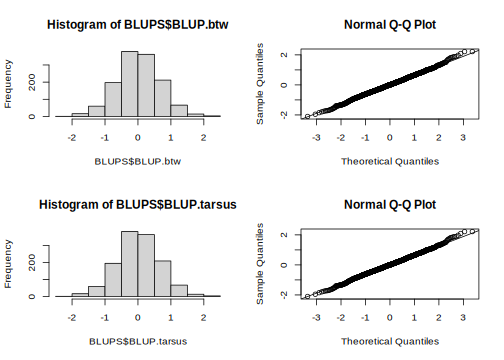
\includegraphics{wam_tuto_files/figure-latex/unnamed-chunk-105-1.pdf}

\begin{Shaded}
\begin{Highlighting}[]
\CommentTok{\#}
\KeywordTok{plot}\NormalTok{(BLUP.tarsus}\OperatorTok{\textasciitilde{}}\NormalTok{BLUP.btw,BLUPS,}\DataTypeTok{xlab=}\StringTok{""}\NormalTok{,}\DataTypeTok{ylab=}\StringTok{""}\NormalTok{, }\DataTypeTok{las=}\FloatTok{1.2}\NormalTok{, }\DataTypeTok{bty=}\StringTok{"o"}\NormalTok{, }\DataTypeTok{col=}\StringTok{"white"}\NormalTok{, }\DataTypeTok{ylim=}\KeywordTok{c}\NormalTok{(}\OperatorTok{{-}}\DecValTok{4}\NormalTok{,}\DecValTok{4}\NormalTok{),}\DataTypeTok{xlim=}\KeywordTok{c}\NormalTok{(}\OperatorTok{{-}}\DecValTok{4}\NormalTok{,}\DecValTok{4}\NormalTok{))}
\KeywordTok{arrows}\NormalTok{(}\DataTypeTok{x0=}\NormalTok{BLUPS}\OperatorTok{$}\NormalTok{BLUP.btw,}\DataTypeTok{y0=}\NormalTok{BLUPS}\OperatorTok{$}\NormalTok{CI.L.tarsus,}\DataTypeTok{x1=}\NormalTok{BLUPS}\OperatorTok{$}\NormalTok{BLUP.btw,}\DataTypeTok{y1=}\NormalTok{BLUPS}\OperatorTok{$}\NormalTok{CI.U.tarsus,}\DataTypeTok{col=}\StringTok{"black"}\NormalTok{,}\DataTypeTok{code=}\DecValTok{3}\NormalTok{,}\DataTypeTok{angle=}\DecValTok{90}\NormalTok{,}\DataTypeTok{length=}\DecValTok{0}\NormalTok{)}
\KeywordTok{arrows}\NormalTok{(}\DataTypeTok{x0=}\NormalTok{BLUPS}\OperatorTok{$}\NormalTok{CI.L.btw,}\DataTypeTok{y0=}\NormalTok{BLUPS}\OperatorTok{$}\NormalTok{BLUP.tarsus,}\DataTypeTok{x1=}\NormalTok{BLUPS}\OperatorTok{$}\NormalTok{CI.U.btw,}\DataTypeTok{y1=}\NormalTok{BLUPS}\OperatorTok{$}\NormalTok{BLUP.tarsus,}\DataTypeTok{col=}\StringTok{"black"}\NormalTok{,}\DataTypeTok{code=}\DecValTok{3}\NormalTok{,}\DataTypeTok{angle=}\DecValTok{90}\NormalTok{,}\DataTypeTok{length=}\DecValTok{0}\NormalTok{)}
\KeywordTok{points}\NormalTok{(BLUP.tarsus}\OperatorTok{\textasciitilde{}}\NormalTok{BLUP.btw,BLUPS,}\DataTypeTok{pch=}\DecValTok{16}\NormalTok{,}\DataTypeTok{col=}\StringTok{"red"}\NormalTok{, }\DataTypeTok{cex=}\FloatTok{1.5}\NormalTok{)}
\KeywordTok{points}\NormalTok{(BLUP.tarsus}\OperatorTok{\textasciitilde{}}\NormalTok{BLUP.btw,BLUPS,}\DataTypeTok{pch=}\DecValTok{1}\NormalTok{, }\DataTypeTok{col=}\KeywordTok{rgb}\NormalTok{(}\DecValTok{0}\NormalTok{,}\DecValTok{0}\NormalTok{,}\DecValTok{0}\NormalTok{,}\FloatTok{0.3}\NormalTok{), }\DataTypeTok{cex=}\KeywordTok{c}\NormalTok{(}\FloatTok{1.5}\NormalTok{))}
\KeywordTok{mtext}\NormalTok{(}\StringTok{"btw (BV±SE)"}\NormalTok{,  }\DataTypeTok{side=}\DecValTok{1}\NormalTok{, }\DataTypeTok{line=}\FloatTok{2.4}\NormalTok{)}
\KeywordTok{mtext}\NormalTok{(}\StringTok{"tarsus (BV±SE)"}\NormalTok{,  }\DataTypeTok{side=}\DecValTok{2}\NormalTok{, }\DataTypeTok{line=}\DecValTok{2}\NormalTok{,}\DataTypeTok{las=}\DecValTok{3}\NormalTok{)}
\end{Highlighting}
\end{Shaded}

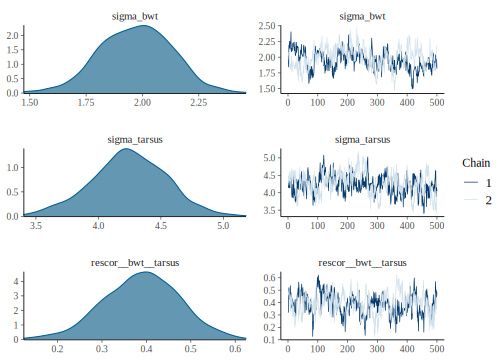
\includegraphics{wam_tuto_files/figure-latex/unnamed-chunk-105-2.pdf}

\hypertarget{partitioning-covariances}{%
\subsection{Partitioning (co)variances}\label{partitioning-covariances}}

As in the tutorial 1, it is possible to partition the variance-covariance matrix between groups (here sex)

\begin{Shaded}
\begin{Highlighting}[]
\NormalTok{prior2}\FloatTok{.3}\NormalTok{ \textless{}{-}}\StringTok{ }\KeywordTok{list}\NormalTok{(}
  \DataTypeTok{G =} \KeywordTok{list}\NormalTok{(}
    \DataTypeTok{G1 =} \KeywordTok{list}\NormalTok{(}\DataTypeTok{V =} \KeywordTok{diag}\NormalTok{(}\DecValTok{2}\NormalTok{), }\DataTypeTok{nu =} \FloatTok{1.002}\NormalTok{),}
    \DataTypeTok{G2 =} \KeywordTok{list}\NormalTok{(}\DataTypeTok{V =} \KeywordTok{diag}\NormalTok{(}\DecValTok{2}\NormalTok{), }\DataTypeTok{nu =} \FloatTok{1.002}\NormalTok{),}
    \DataTypeTok{G3 =} \KeywordTok{list}\NormalTok{(}\DataTypeTok{V =} \KeywordTok{diag}\NormalTok{(}\DecValTok{2}\NormalTok{), }\DataTypeTok{nu =} \FloatTok{1.002}\NormalTok{),}
    \DataTypeTok{G4 =} \KeywordTok{list}\NormalTok{(}\DataTypeTok{V =} \KeywordTok{diag}\NormalTok{(}\DecValTok{2}\NormalTok{), }\DataTypeTok{nu =} \FloatTok{1.002}\NormalTok{)}
\NormalTok{  ),}
  \DataTypeTok{R =} \KeywordTok{list}\NormalTok{(}
    \DataTypeTok{V1 =} \KeywordTok{list}\NormalTok{(}\DataTypeTok{V =} \KeywordTok{diag}\NormalTok{(}\DecValTok{2}\NormalTok{), }\DataTypeTok{nu =} \FloatTok{1.002}\NormalTok{),}
    \DataTypeTok{V2 =} \KeywordTok{list}\NormalTok{(}\DataTypeTok{V =} \KeywordTok{diag}\NormalTok{(}\DecValTok{2}\NormalTok{), }\DataTypeTok{nu =} \FloatTok{1.002}\NormalTok{)}
\NormalTok{  )}
\NormalTok{)}

\NormalTok{model2}\FloatTok{.4}\NormalTok{ \textless{}{-}}\StringTok{ }\KeywordTok{MCMCglmm}\NormalTok{(}\KeywordTok{cbind}\NormalTok{(bwt, tarsus) }\OperatorTok{\textasciitilde{}}\StringTok{ }\NormalTok{trait }\OperatorTok{{-}}\StringTok{ }\DecValTok{1} \OperatorTok{+}\StringTok{ }\NormalTok{trait}\OperatorTok{:}\NormalTok{sex,}
  \DataTypeTok{random =} \OperatorTok{\textasciitilde{}}\StringTok{ }\KeywordTok{us}\NormalTok{(}\KeywordTok{at.level}\NormalTok{(sex, }\StringTok{"1"}\NormalTok{)}\OperatorTok{:}\NormalTok{trait)}\OperatorTok{:}\NormalTok{animal }\OperatorTok{+}\StringTok{ }\KeywordTok{us}\NormalTok{(}\KeywordTok{at.level}\NormalTok{(sex, }\StringTok{"2"}\NormalTok{)}\OperatorTok{:}\NormalTok{trait)}\OperatorTok{:}\NormalTok{animal }\OperatorTok{+}\StringTok{ }\KeywordTok{us}\NormalTok{(trait)}\OperatorTok{:}\NormalTok{byear }\OperatorTok{+}\StringTok{ }\KeywordTok{us}\NormalTok{(trait)}\OperatorTok{:}\NormalTok{mother,}
  \DataTypeTok{rcov =} \OperatorTok{\textasciitilde{}}\StringTok{ }\KeywordTok{us}\NormalTok{(}\KeywordTok{at.level}\NormalTok{(sex, }\StringTok{"1"}\NormalTok{)}\OperatorTok{:}\NormalTok{trait)}\OperatorTok{:}\NormalTok{units }\OperatorTok{+}\StringTok{ }\KeywordTok{us}\NormalTok{(}\KeywordTok{at.level}\NormalTok{(sex, }\StringTok{"2"}\NormalTok{)}\OperatorTok{:}\NormalTok{trait)}\OperatorTok{:}\NormalTok{units,}
  \DataTypeTok{family =} \KeywordTok{c}\NormalTok{(}\StringTok{"gaussian"}\NormalTok{, }\StringTok{"gaussian"}\NormalTok{),}
  \DataTypeTok{ginv =} \KeywordTok{list}\NormalTok{(}\DataTypeTok{animal =}\NormalTok{ Ainv), }\DataTypeTok{data =}\NormalTok{ gryphon,}
  \DataTypeTok{nitt =} \DecValTok{130000}\NormalTok{, }\DataTypeTok{thin =} \DecValTok{100}\NormalTok{, }\DataTypeTok{burnin =} \DecValTok{30000}\NormalTok{,}
  \DataTypeTok{prior =}\NormalTok{ prior2}\FloatTok{.3}\NormalTok{, }\DataTypeTok{verbose =} \OtherTok{FALSE}\NormalTok{, }\DataTypeTok{pr=}\OtherTok{TRUE}\NormalTok{,}
\NormalTok{)}
\KeywordTok{save}\NormalTok{(model2}\FloatTok{.4}\NormalTok{, }\DataTypeTok{file =} \StringTok{"data/MCMCglmm\_model2\_4\_LongRun.rda"}\NormalTok{)}
\end{Highlighting}
\end{Shaded}

Again we have provided the data from one such run. It can be accessed using the code:

\begin{Shaded}
\begin{Highlighting}[]
\KeywordTok{load}\NormalTok{(}\DataTypeTok{file =} \StringTok{"data/MCMCglmm\_model2\_4\_LongRun.rda"}\NormalTok{)}
\KeywordTok{summary}\NormalTok{(model2}\FloatTok{.4}\NormalTok{)}
\end{Highlighting}
\end{Shaded}

\begin{verbatim}
## 
##  Iterations = 30001:129901
##  Thinning interval  = 100
##  Sample size  = 1000 
## 
##  DIC: 5781.353 
## 
##  G-structure:  ~us(at.level(sex, "1"):trait):animal
## 
##                                                                      post.mean
## at.level(sex, "1"):traitbwt:at.level(sex, "1"):traitbwt.animal           1.309
## at.level(sex, "1"):traittarsus:at.level(sex, "1"):traitbwt.animal        1.732
## at.level(sex, "1"):traitbwt:at.level(sex, "1"):traittarsus.animal        1.732
## at.level(sex, "1"):traittarsus:at.level(sex, "1"):traittarsus.animal     4.632
##                                                                      l-95% CI
## at.level(sex, "1"):traitbwt:at.level(sex, "1"):traitbwt.animal        0.30628
## at.level(sex, "1"):traittarsus:at.level(sex, "1"):traitbwt.animal     0.01207
## at.level(sex, "1"):traitbwt:at.level(sex, "1"):traittarsus.animal     0.01207
## at.level(sex, "1"):traittarsus:at.level(sex, "1"):traittarsus.animal  0.31760
##                                                                      u-95% CI
## at.level(sex, "1"):traitbwt:at.level(sex, "1"):traitbwt.animal          2.403
## at.level(sex, "1"):traittarsus:at.level(sex, "1"):traitbwt.animal       3.957
## at.level(sex, "1"):traitbwt:at.level(sex, "1"):traittarsus.animal       3.957
## at.level(sex, "1"):traittarsus:at.level(sex, "1"):traittarsus.animal   10.415
##                                                                      eff.samp
## at.level(sex, "1"):traitbwt:at.level(sex, "1"):traitbwt.animal          275.9
## at.level(sex, "1"):traittarsus:at.level(sex, "1"):traitbwt.animal       188.6
## at.level(sex, "1"):traitbwt:at.level(sex, "1"):traittarsus.animal       188.6
## at.level(sex, "1"):traittarsus:at.level(sex, "1"):traittarsus.animal    116.1
## 
##                ~us(at.level(sex, "2"):trait):animal
## 
##                                                                      post.mean
## at.level(sex, "2"):traitbwt:at.level(sex, "2"):traitbwt.animal           2.542
## at.level(sex, "2"):traittarsus:at.level(sex, "2"):traitbwt.animal        6.343
## at.level(sex, "2"):traitbwt:at.level(sex, "2"):traittarsus.animal        6.343
## at.level(sex, "2"):traittarsus:at.level(sex, "2"):traittarsus.animal    19.987
##                                                                      l-95% CI
## at.level(sex, "2"):traitbwt:at.level(sex, "2"):traitbwt.animal          1.048
## at.level(sex, "2"):traittarsus:at.level(sex, "2"):traitbwt.animal       1.746
## at.level(sex, "2"):traitbwt:at.level(sex, "2"):traittarsus.animal       1.746
## at.level(sex, "2"):traittarsus:at.level(sex, "2"):traittarsus.animal    5.544
##                                                                      u-95% CI
## at.level(sex, "2"):traitbwt:at.level(sex, "2"):traitbwt.animal          4.194
## at.level(sex, "2"):traittarsus:at.level(sex, "2"):traitbwt.animal       9.571
## at.level(sex, "2"):traitbwt:at.level(sex, "2"):traittarsus.animal       9.571
## at.level(sex, "2"):traittarsus:at.level(sex, "2"):traittarsus.animal   29.561
##                                                                      eff.samp
## at.level(sex, "2"):traitbwt:at.level(sex, "2"):traitbwt.animal         118.48
## at.level(sex, "2"):traittarsus:at.level(sex, "2"):traitbwt.animal       83.91
## at.level(sex, "2"):traitbwt:at.level(sex, "2"):traittarsus.animal       83.91
## at.level(sex, "2"):traittarsus:at.level(sex, "2"):traittarsus.animal    70.87
## 
##                ~us(trait):byear
## 
##                               post.mean l-95% CI u-95% CI eff.samp
## traitbwt:traitbwt.byear          1.0665   0.5056    1.690     1193
## traittarsus:traitbwt.byear       0.1562  -0.7425    1.091      846
## traitbwt:traittarsus.byear       0.1562  -0.7425    1.091      846
## traittarsus:traittarsus.byear    4.3061   2.0966    7.661     1000
## 
##                ~us(trait):mother
## 
##                                post.mean l-95% CI u-95% CI eff.samp
## traitbwt:traitbwt.mother           1.344   0.9056   1.8031    683.4
## traittarsus:traitbwt.mother       -1.568  -2.2064  -0.9099    420.9
## traitbwt:traittarsus.mother       -1.568  -2.2064  -0.9099    420.9
## traittarsus:traittarsus.mother     4.471   2.3931   6.8389    502.2
## 
##  R-structure:  ~us(at.level(sex, "1"):trait):units
## 
##                                                                     post.mean
## at.level(sex, "1"):traitbwt:at.level(sex, "1"):traitbwt.units           2.424
## at.level(sex, "1"):traittarsus:at.level(sex, "1"):traitbwt.units        5.071
## at.level(sex, "1"):traitbwt:at.level(sex, "1"):traittarsus.units        5.071
## at.level(sex, "1"):traittarsus:at.level(sex, "1"):traittarsus.units    15.138
##                                                                     l-95% CI
## at.level(sex, "1"):traitbwt:at.level(sex, "1"):traitbwt.units          1.362
## at.level(sex, "1"):traittarsus:at.level(sex, "1"):traitbwt.units       3.039
## at.level(sex, "1"):traitbwt:at.level(sex, "1"):traittarsus.units       3.039
## at.level(sex, "1"):traittarsus:at.level(sex, "1"):traittarsus.units    9.432
##                                                                     u-95% CI
## at.level(sex, "1"):traitbwt:at.level(sex, "1"):traitbwt.units          3.356
## at.level(sex, "1"):traittarsus:at.level(sex, "1"):traitbwt.units       7.027
## at.level(sex, "1"):traitbwt:at.level(sex, "1"):traittarsus.units       7.027
## at.level(sex, "1"):traittarsus:at.level(sex, "1"):traittarsus.units   20.904
##                                                                     eff.samp
## at.level(sex, "1"):traitbwt:at.level(sex, "1"):traitbwt.units          319.3
## at.level(sex, "1"):traittarsus:at.level(sex, "1"):traitbwt.units       161.9
## at.level(sex, "1"):traitbwt:at.level(sex, "1"):traittarsus.units       161.9
## at.level(sex, "1"):traittarsus:at.level(sex, "1"):traittarsus.units    146.7
## 
##                ~us(at.level(sex, "2"):trait):units
## 
##                                                                     post.mean
## at.level(sex, "2"):traitbwt:at.level(sex, "2"):traitbwt.units           1.259
## at.level(sex, "2"):traittarsus:at.level(sex, "2"):traitbwt.units        1.595
## at.level(sex, "2"):traitbwt:at.level(sex, "2"):traittarsus.units        1.595
## at.level(sex, "2"):traittarsus:at.level(sex, "2"):traittarsus.units     5.700
##                                                                     l-95% CI
## at.level(sex, "2"):traitbwt:at.level(sex, "2"):traitbwt.units         0.2235
## at.level(sex, "2"):traittarsus:at.level(sex, "2"):traitbwt.units     -0.6282
## at.level(sex, "2"):traitbwt:at.level(sex, "2"):traittarsus.units     -0.6282
## at.level(sex, "2"):traittarsus:at.level(sex, "2"):traittarsus.units   0.0998
##                                                                     u-95% CI
## at.level(sex, "2"):traitbwt:at.level(sex, "2"):traitbwt.units          2.624
## at.level(sex, "2"):traittarsus:at.level(sex, "2"):traitbwt.units       5.238
## at.level(sex, "2"):traitbwt:at.level(sex, "2"):traittarsus.units       5.238
## at.level(sex, "2"):traittarsus:at.level(sex, "2"):traittarsus.units   16.890
##                                                                     eff.samp
## at.level(sex, "2"):traitbwt:at.level(sex, "2"):traitbwt.units         107.05
## at.level(sex, "2"):traittarsus:at.level(sex, "2"):traitbwt.units       75.15
## at.level(sex, "2"):traitbwt:at.level(sex, "2"):traittarsus.units       75.15
## at.level(sex, "2"):traittarsus:at.level(sex, "2"):traittarsus.units    65.01
## 
##  Location effects: cbind(bwt, tarsus) ~ trait - 1 + trait:sex 
## 
##                  post.mean l-95% CI u-95% CI eff.samp  pMCMC    
## traitbwt           6.37918  5.91126  6.83434    805.9 <0.001 ***
## traittarsus       20.58772 19.68033 21.64950   1000.0 <0.001 ***
## traitbwt:sex2      1.94258  1.59412  2.31172   1107.5 <0.001 ***
## traittarsus:sex2  -0.06608 -1.01248  0.81828   1000.0  0.888    
## ---
## Signif. codes:  0 '***' 0.001 '**' 0.01 '*' 0.05 '.' 0.1 ' ' 1
\end{verbatim}

\begin{Shaded}
\begin{Highlighting}[]
\KeywordTok{autocorr}\NormalTok{(model2}\FloatTok{.4}\OperatorTok{$}\NormalTok{VCV)}
\end{Highlighting}
\end{Shaded}

\begin{verbatim}
## , , at.level(sex, "1"):traitbwt:at.level(sex, "1"):traitbwt.animal
## 
##          at.level(sex, "1"):traitbwt:at.level(sex, "1"):traitbwt.animal
## Lag 0                                                        1.00000000
## Lag 100                                                      0.53245307
## Lag 500                                                      0.12686054
## Lag 1000                                                     0.06237696
## Lag 5000                                                     0.01824033
##          at.level(sex, "1"):traittarsus:at.level(sex, "1"):traitbwt.animal
## Lag 0                                                          0.793591491
## Lag 100                                                        0.463650796
## Lag 500                                                        0.144349339
## Lag 1000                                                       0.123875583
## Lag 5000                                                       0.002943118
##          at.level(sex, "1"):traitbwt:at.level(sex, "1"):traittarsus.animal
## Lag 0                                                          0.793591491
## Lag 100                                                        0.463650796
## Lag 500                                                        0.144349339
## Lag 1000                                                       0.123875583
## Lag 5000                                                       0.002943118
##          at.level(sex, "1"):traittarsus:at.level(sex, "1"):traittarsus.animal
## Lag 0                                                             0.491321854
## Lag 100                                                           0.327568418
## Lag 500                                                           0.153728089
## Lag 1000                                                          0.164417478
## Lag 5000                                                          0.009502224
##          at.level(sex, "2"):traitbwt:at.level(sex, "2"):traitbwt.animal
## Lag 0                                                      -0.003843723
## Lag 100                                                    -0.057261889
## Lag 500                                                    -0.108913061
## Lag 1000                                                   -0.047889583
## Lag 5000                                                    0.052420824
##          at.level(sex, "2"):traittarsus:at.level(sex, "2"):traitbwt.animal
## Lag 0                                                          -0.08612408
## Lag 100                                                        -0.11380506
## Lag 500                                                        -0.12380683
## Lag 1000                                                       -0.05287906
## Lag 5000                                                        0.02599475
##          at.level(sex, "2"):traitbwt:at.level(sex, "2"):traittarsus.animal
## Lag 0                                                          -0.08612408
## Lag 100                                                        -0.11380506
## Lag 500                                                        -0.12380683
## Lag 1000                                                       -0.05287906
## Lag 5000                                                        0.02599475
##          at.level(sex, "2"):traittarsus:at.level(sex, "2"):traittarsus.animal
## Lag 0                                                             -0.11625878
## Lag 100                                                           -0.12093127
## Lag 500                                                           -0.09830795
## Lag 1000                                                          -0.05398243
## Lag 5000                                                           0.01854725
##          traitbwt:traitbwt.byear traittarsus:traitbwt.byear
## Lag 0               0.0329574997                -0.01270192
## Lag 100            -0.0004022758                -0.01069124
## Lag 500             0.0108756691                -0.03078252
## Lag 1000           -0.0402453374                -0.05525656
## Lag 5000           -0.0094617871                 0.01181511
##          traitbwt:traittarsus.byear traittarsus:traittarsus.byear
## Lag 0                   -0.01270192                  -0.002678407
## Lag 100                 -0.01069124                   0.030235120
## Lag 500                 -0.03078252                   0.039658918
## Lag 1000                -0.05525656                  -0.013352341
## Lag 5000                 0.01181511                  -0.014747793
##          traitbwt:traitbwt.mother traittarsus:traitbwt.mother
## Lag 0                 -0.22299692                 -0.11473447
## Lag 100               -0.14281206                 -0.08858053
## Lag 500               -0.04546466                  0.01664463
## Lag 1000              -0.01935302                 -0.02792684
## Lag 5000              -0.02375293                  0.03638036
##          traitbwt:traittarsus.mother traittarsus:traittarsus.mother
## Lag 0                    -0.11473447                    0.077005136
## Lag 100                  -0.08858053                    0.047410051
## Lag 500                   0.01664463                    0.063839298
## Lag 1000                 -0.02792684                   -0.005369024
## Lag 5000                  0.03638036                   -0.045393729
##          at.level(sex, "1"):traitbwt:at.level(sex, "1"):traitbwt.units
## Lag 0                                                      -0.80762218
## Lag 100                                                    -0.48377693
## Lag 500                                                    -0.11906060
## Lag 1000                                                   -0.08092305
## Lag 5000                                                   -0.01474778
##          at.level(sex, "1"):traittarsus:at.level(sex, "1"):traitbwt.units
## Lag 0                                                        -0.637966294
## Lag 100                                                      -0.415484170
## Lag 500                                                      -0.155520020
## Lag 1000                                                     -0.133950450
## Lag 5000                                                     -0.006204077
##          at.level(sex, "1"):traitbwt:at.level(sex, "1"):traittarsus.units
## Lag 0                                                        -0.637966294
## Lag 100                                                      -0.415484170
## Lag 500                                                      -0.155520020
## Lag 1000                                                     -0.133950450
## Lag 5000                                                     -0.006204077
##          at.level(sex, "1"):traittarsus:at.level(sex, "1"):traittarsus.units
## Lag 0                                                           -0.412524277
## Lag 100                                                         -0.303401540
## Lag 500                                                         -0.183526418
## Lag 1000                                                        -0.155534598
## Lag 5000                                                        -0.009036592
##          at.level(sex, "2"):traitbwt:at.level(sex, "2"):traitbwt.units
## Lag 0                                                       0.04046100
## Lag 100                                                     0.08263080
## Lag 500                                                     0.12012062
## Lag 1000                                                    0.05230390
## Lag 5000                                                   -0.05042002
##          at.level(sex, "2"):traittarsus:at.level(sex, "2"):traitbwt.units
## Lag 0                                                          0.10738222
## Lag 100                                                        0.12852079
## Lag 500                                                        0.12878991
## Lag 1000                                                       0.06253120
## Lag 5000                                                      -0.02977866
##          at.level(sex, "2"):traitbwt:at.level(sex, "2"):traittarsus.units
## Lag 0                                                          0.10738222
## Lag 100                                                        0.12852079
## Lag 500                                                        0.12878991
## Lag 1000                                                       0.06253120
## Lag 5000                                                      -0.02977866
##          at.level(sex, "2"):traittarsus:at.level(sex, "2"):traittarsus.units
## Lag 0                                                             0.12157763
## Lag 100                                                           0.13000823
## Lag 500                                                           0.10069977
## Lag 1000                                                          0.05608494
## Lag 5000                                                         -0.02159746
## 
## , , at.level(sex, "1"):traittarsus:at.level(sex, "1"):traitbwt.animal
## 
##          at.level(sex, "1"):traitbwt:at.level(sex, "1"):traitbwt.animal
## Lag 0                                                        0.79359149
## Lag 100                                                      0.47105949
## Lag 500                                                      0.12122685
## Lag 1000                                                     0.06563711
## Lag 5000                                                     0.02614113
##          at.level(sex, "1"):traittarsus:at.level(sex, "1"):traitbwt.animal
## Lag 0                                                            1.0000000
## Lag 100                                                          0.6458216
## Lag 500                                                          0.2191270
## Lag 1000                                                         0.1407425
## Lag 5000                                                         0.0165183
##          at.level(sex, "1"):traitbwt:at.level(sex, "1"):traittarsus.animal
## Lag 0                                                            1.0000000
## Lag 100                                                          0.6458216
## Lag 500                                                          0.2191270
## Lag 1000                                                         0.1407425
## Lag 5000                                                         0.0165183
##          at.level(sex, "1"):traittarsus:at.level(sex, "1"):traittarsus.animal
## Lag 0                                                              0.85123642
## Lag 100                                                            0.60842535
## Lag 500                                                            0.25356361
## Lag 1000                                                           0.18179651
## Lag 5000                                                           0.05340421
##          at.level(sex, "2"):traitbwt:at.level(sex, "2"):traitbwt.animal
## Lag 0                                                       -0.07587185
## Lag 100                                                     -0.10484483
## Lag 500                                                     -0.12899421
## Lag 1000                                                    -0.04675813
## Lag 5000                                                     0.05371834
##          at.level(sex, "2"):traittarsus:at.level(sex, "2"):traitbwt.animal
## Lag 0                                                          -0.10066538
## Lag 100                                                        -0.11984034
## Lag 500                                                        -0.10860036
## Lag 1000                                                       -0.04404039
## Lag 5000                                                        0.03404106
##          at.level(sex, "2"):traitbwt:at.level(sex, "2"):traittarsus.animal
## Lag 0                                                          -0.10066538
## Lag 100                                                        -0.11984034
## Lag 500                                                        -0.10860036
## Lag 1000                                                       -0.04404039
## Lag 5000                                                        0.03404106
##          at.level(sex, "2"):traittarsus:at.level(sex, "2"):traittarsus.animal
## Lag 0                                                             -0.08130370
## Lag 100                                                           -0.08739523
## Lag 500                                                           -0.06222808
## Lag 1000                                                          -0.02757986
## Lag 5000                                                           0.02334607
##          traitbwt:traitbwt.byear traittarsus:traitbwt.byear
## Lag 0               -0.004800874                -0.04707976
## Lag 100             -0.008011503                -0.02692482
## Lag 500              0.003485631                -0.02204639
## Lag 1000            -0.038554146                -0.05647478
## Lag 5000            -0.005966844                 0.01256057
##          traitbwt:traittarsus.byear traittarsus:traittarsus.byear
## Lag 0                   -0.04707976                  -0.023318437
## Lag 100                 -0.02692482                   0.007533592
## Lag 500                 -0.02204639                   0.024968239
## Lag 1000                -0.05647478                  -0.009582103
## Lag 5000                 0.01256057                   0.005864905
##          traitbwt:traitbwt.mother traittarsus:traitbwt.mother
## Lag 0                 -0.13866371                -0.172461577
## Lag 100               -0.07597941                -0.127399110
## Lag 500               -0.04943607                -0.039757470
## Lag 1000              -0.02804419                -0.046223598
## Lag 5000              -0.02328241                -0.005813647
##          traitbwt:traittarsus.mother traittarsus:traittarsus.mother
## Lag 0                   -0.172461577                    0.025486576
## Lag 100                 -0.127399110                    0.015476585
## Lag 500                 -0.039757470                   -0.002678799
## Lag 1000                -0.046223598                   -0.037182954
## Lag 5000                -0.005813647                   -0.013258339
##          at.level(sex, "1"):traitbwt:at.level(sex, "1"):traitbwt.units
## Lag 0                                                     -0.662342828
## Lag 100                                                   -0.445416218
## Lag 500                                                   -0.096469432
## Lag 1000                                                  -0.072047578
## Lag 5000                                                  -0.002333197
##          at.level(sex, "1"):traittarsus:at.level(sex, "1"):traitbwt.units
## Lag 0                                                         -0.79740796
## Lag 100                                                       -0.56365504
## Lag 500                                                       -0.18875545
## Lag 1000                                                      -0.12573197
## Lag 5000                                                      -0.01529201
##          at.level(sex, "1"):traitbwt:at.level(sex, "1"):traittarsus.units
## Lag 0                                                         -0.79740796
## Lag 100                                                       -0.56365504
## Lag 500                                                       -0.18875545
## Lag 1000                                                      -0.12573197
## Lag 5000                                                      -0.01529201
##          at.level(sex, "1"):traittarsus:at.level(sex, "1"):traittarsus.units
## Lag 0                                                            -0.69413392
## Lag 100                                                          -0.53055234
## Lag 500                                                          -0.23504465
## Lag 1000                                                         -0.14414582
## Lag 5000                                                         -0.06176488
##          at.level(sex, "2"):traitbwt:at.level(sex, "2"):traitbwt.units
## Lag 0                                                       0.09874742
## Lag 100                                                     0.12012793
## Lag 500                                                     0.13963436
## Lag 1000                                                    0.04225527
## Lag 5000                                                   -0.06006498
##          at.level(sex, "2"):traittarsus:at.level(sex, "2"):traitbwt.units
## Lag 0                                                          0.12036344
## Lag 100                                                        0.13016686
## Lag 500                                                        0.11898560
## Lag 1000                                                       0.04600190
## Lag 5000                                                      -0.04060248
##          at.level(sex, "2"):traitbwt:at.level(sex, "2"):traittarsus.units
## Lag 0                                                          0.12036344
## Lag 100                                                        0.13016686
## Lag 500                                                        0.11898560
## Lag 1000                                                       0.04600190
## Lag 5000                                                      -0.04060248
##          at.level(sex, "2"):traittarsus:at.level(sex, "2"):traittarsus.units
## Lag 0                                                             0.09081352
## Lag 100                                                           0.09525252
## Lag 500                                                           0.06993879
## Lag 1000                                                          0.03023552
## Lag 5000                                                         -0.02979182
## 
## , , at.level(sex, "1"):traitbwt:at.level(sex, "1"):traittarsus.animal
## 
##          at.level(sex, "1"):traitbwt:at.level(sex, "1"):traitbwt.animal
## Lag 0                                                        0.79359149
## Lag 100                                                      0.47105949
## Lag 500                                                      0.12122685
## Lag 1000                                                     0.06563711
## Lag 5000                                                     0.02614113
##          at.level(sex, "1"):traittarsus:at.level(sex, "1"):traitbwt.animal
## Lag 0                                                            1.0000000
## Lag 100                                                          0.6458216
## Lag 500                                                          0.2191270
## Lag 1000                                                         0.1407425
## Lag 5000                                                         0.0165183
##          at.level(sex, "1"):traitbwt:at.level(sex, "1"):traittarsus.animal
## Lag 0                                                            1.0000000
## Lag 100                                                          0.6458216
## Lag 500                                                          0.2191270
## Lag 1000                                                         0.1407425
## Lag 5000                                                         0.0165183
##          at.level(sex, "1"):traittarsus:at.level(sex, "1"):traittarsus.animal
## Lag 0                                                              0.85123642
## Lag 100                                                            0.60842535
## Lag 500                                                            0.25356361
## Lag 1000                                                           0.18179651
## Lag 5000                                                           0.05340421
##          at.level(sex, "2"):traitbwt:at.level(sex, "2"):traitbwt.animal
## Lag 0                                                       -0.07587185
## Lag 100                                                     -0.10484483
## Lag 500                                                     -0.12899421
## Lag 1000                                                    -0.04675813
## Lag 5000                                                     0.05371834
##          at.level(sex, "2"):traittarsus:at.level(sex, "2"):traitbwt.animal
## Lag 0                                                          -0.10066538
## Lag 100                                                        -0.11984034
## Lag 500                                                        -0.10860036
## Lag 1000                                                       -0.04404039
## Lag 5000                                                        0.03404106
##          at.level(sex, "2"):traitbwt:at.level(sex, "2"):traittarsus.animal
## Lag 0                                                          -0.10066538
## Lag 100                                                        -0.11984034
## Lag 500                                                        -0.10860036
## Lag 1000                                                       -0.04404039
## Lag 5000                                                        0.03404106
##          at.level(sex, "2"):traittarsus:at.level(sex, "2"):traittarsus.animal
## Lag 0                                                             -0.08130370
## Lag 100                                                           -0.08739523
## Lag 500                                                           -0.06222808
## Lag 1000                                                          -0.02757986
## Lag 5000                                                           0.02334607
##          traitbwt:traitbwt.byear traittarsus:traitbwt.byear
## Lag 0               -0.004800874                -0.04707976
## Lag 100             -0.008011503                -0.02692482
## Lag 500              0.003485631                -0.02204639
## Lag 1000            -0.038554146                -0.05647478
## Lag 5000            -0.005966844                 0.01256057
##          traitbwt:traittarsus.byear traittarsus:traittarsus.byear
## Lag 0                   -0.04707976                  -0.023318437
## Lag 100                 -0.02692482                   0.007533592
## Lag 500                 -0.02204639                   0.024968239
## Lag 1000                -0.05647478                  -0.009582103
## Lag 5000                 0.01256057                   0.005864905
##          traitbwt:traitbwt.mother traittarsus:traitbwt.mother
## Lag 0                 -0.13866371                -0.172461577
## Lag 100               -0.07597941                -0.127399110
## Lag 500               -0.04943607                -0.039757470
## Lag 1000              -0.02804419                -0.046223598
## Lag 5000              -0.02328241                -0.005813647
##          traitbwt:traittarsus.mother traittarsus:traittarsus.mother
## Lag 0                   -0.172461577                    0.025486576
## Lag 100                 -0.127399110                    0.015476585
## Lag 500                 -0.039757470                   -0.002678799
## Lag 1000                -0.046223598                   -0.037182954
## Lag 5000                -0.005813647                   -0.013258339
##          at.level(sex, "1"):traitbwt:at.level(sex, "1"):traitbwt.units
## Lag 0                                                     -0.662342828
## Lag 100                                                   -0.445416218
## Lag 500                                                   -0.096469432
## Lag 1000                                                  -0.072047578
## Lag 5000                                                  -0.002333197
##          at.level(sex, "1"):traittarsus:at.level(sex, "1"):traitbwt.units
## Lag 0                                                         -0.79740796
## Lag 100                                                       -0.56365504
## Lag 500                                                       -0.18875545
## Lag 1000                                                      -0.12573197
## Lag 5000                                                      -0.01529201
##          at.level(sex, "1"):traitbwt:at.level(sex, "1"):traittarsus.units
## Lag 0                                                         -0.79740796
## Lag 100                                                       -0.56365504
## Lag 500                                                       -0.18875545
## Lag 1000                                                      -0.12573197
## Lag 5000                                                      -0.01529201
##          at.level(sex, "1"):traittarsus:at.level(sex, "1"):traittarsus.units
## Lag 0                                                            -0.69413392
## Lag 100                                                          -0.53055234
## Lag 500                                                          -0.23504465
## Lag 1000                                                         -0.14414582
## Lag 5000                                                         -0.06176488
##          at.level(sex, "2"):traitbwt:at.level(sex, "2"):traitbwt.units
## Lag 0                                                       0.09874742
## Lag 100                                                     0.12012793
## Lag 500                                                     0.13963436
## Lag 1000                                                    0.04225527
## Lag 5000                                                   -0.06006498
##          at.level(sex, "2"):traittarsus:at.level(sex, "2"):traitbwt.units
## Lag 0                                                          0.12036344
## Lag 100                                                        0.13016686
## Lag 500                                                        0.11898560
## Lag 1000                                                       0.04600190
## Lag 5000                                                      -0.04060248
##          at.level(sex, "2"):traitbwt:at.level(sex, "2"):traittarsus.units
## Lag 0                                                          0.12036344
## Lag 100                                                        0.13016686
## Lag 500                                                        0.11898560
## Lag 1000                                                       0.04600190
## Lag 5000                                                      -0.04060248
##          at.level(sex, "2"):traittarsus:at.level(sex, "2"):traittarsus.units
## Lag 0                                                             0.09081352
## Lag 100                                                           0.09525252
## Lag 500                                                           0.06993879
## Lag 1000                                                          0.03023552
## Lag 5000                                                         -0.02979182
## 
## , , at.level(sex, "1"):traittarsus:at.level(sex, "1"):traittarsus.animal
## 
##          at.level(sex, "1"):traitbwt:at.level(sex, "1"):traitbwt.animal
## Lag 0                                                        0.49132185
## Lag 100                                                      0.32397350
## Lag 500                                                      0.09735587
## Lag 1000                                                     0.01948632
## Lag 5000                                                     0.01400017
##          at.level(sex, "1"):traittarsus:at.level(sex, "1"):traitbwt.animal
## Lag 0                                                          0.851236420
## Lag 100                                                        0.599217841
## Lag 500                                                        0.236266209
## Lag 1000                                                       0.091814106
## Lag 5000                                                       0.003895014
##          at.level(sex, "1"):traitbwt:at.level(sex, "1"):traittarsus.animal
## Lag 0                                                          0.851236420
## Lag 100                                                        0.599217841
## Lag 500                                                        0.236266209
## Lag 1000                                                       0.091814106
## Lag 5000                                                       0.003895014
##          at.level(sex, "1"):traittarsus:at.level(sex, "1"):traittarsus.animal
## Lag 0                                                              1.00000000
## Lag 100                                                            0.74200065
## Lag 500                                                            0.30091371
## Lag 1000                                                           0.12851708
## Lag 5000                                                           0.04303146
##          at.level(sex, "2"):traitbwt:at.level(sex, "2"):traitbwt.animal
## Lag 0                                                       -0.05845611
## Lag 100                                                     -0.07395684
## Lag 500                                                     -0.11589624
## Lag 1000                                                    -0.04794607
## Lag 5000                                                     0.05750024
##          at.level(sex, "2"):traittarsus:at.level(sex, "2"):traitbwt.animal
## Lag 0                                                          -0.05165271
## Lag 100                                                        -0.06815575
## Lag 500                                                        -0.07284060
## Lag 1000                                                       -0.03823355
## Lag 5000                                                        0.05267309
##          at.level(sex, "2"):traitbwt:at.level(sex, "2"):traittarsus.animal
## Lag 0                                                          -0.05165271
## Lag 100                                                        -0.06815575
## Lag 500                                                        -0.07284060
## Lag 1000                                                       -0.03823355
## Lag 5000                                                        0.05267309
##          at.level(sex, "2"):traittarsus:at.level(sex, "2"):traittarsus.animal
## Lag 0                                                             -0.02909781
## Lag 100                                                           -0.03618871
## Lag 500                                                           -0.02507480
## Lag 1000                                                          -0.01566177
## Lag 5000                                                           0.03620672
##          traitbwt:traitbwt.byear traittarsus:traitbwt.byear
## Lag 0                -0.04518682               -0.053509656
## Lag 100              -0.03023390               -0.053785754
## Lag 500              -0.01167528               -0.030562683
## Lag 1000             -0.03823697               -0.022101926
## Lag 5000             -0.02463048                0.001563628
##          traitbwt:traittarsus.byear traittarsus:traittarsus.byear
## Lag 0                  -0.053509656                  -0.007685252
## Lag 100                -0.053785754                  -0.006306728
## Lag 500                -0.030562683                   0.014291649
## Lag 1000               -0.022101926                  -0.005269219
## Lag 5000                0.001563628                   0.019401666
##          traitbwt:traitbwt.mother traittarsus:traitbwt.mother
## Lag 0                -0.063423241                 -0.17777280
## Lag 100              -0.009062692                 -0.13853865
## Lag 500              -0.042113848                 -0.08286190
## Lag 1000             -0.013957065                 -0.01322478
## Lag 5000              0.006507080                 -0.01155970
##          traitbwt:traittarsus.mother traittarsus:traittarsus.mother
## Lag 0                    -0.17777280                    -0.04728633
## Lag 100                  -0.13853865                    -0.04945451
## Lag 500                  -0.08286190                    -0.03304820
## Lag 1000                 -0.01322478                    -0.01992587
## Lag 5000                 -0.01155970                     0.03384995
##          at.level(sex, "1"):traitbwt:at.level(sex, "1"):traitbwt.units
## Lag 0                                                     -0.409207676
## Lag 100                                                   -0.307288937
## Lag 500                                                   -0.061272231
## Lag 1000                                                  -0.042039590
## Lag 5000                                                   0.008258457
##          at.level(sex, "1"):traittarsus:at.level(sex, "1"):traitbwt.units
## Lag 0                                                        -0.671382738
## Lag 100                                                      -0.510544011
## Lag 500                                                      -0.182950626
## Lag 1000                                                     -0.088268794
## Lag 5000                                                     -0.005387253
##          at.level(sex, "1"):traitbwt:at.level(sex, "1"):traittarsus.units
## Lag 0                                                        -0.671382738
## Lag 100                                                      -0.510544011
## Lag 500                                                      -0.182950626
## Lag 1000                                                     -0.088268794
## Lag 5000                                                     -0.005387253
##          at.level(sex, "1"):traittarsus:at.level(sex, "1"):traittarsus.units
## Lag 0                                                            -0.79571901
## Lag 100                                                          -0.62678280
## Lag 500                                                          -0.25804277
## Lag 1000                                                         -0.10484463
## Lag 5000                                                         -0.05217593
##          at.level(sex, "2"):traitbwt:at.level(sex, "2"):traitbwt.units
## Lag 0                                                       0.06806845
## Lag 100                                                     0.07815045
## Lag 500                                                     0.12138479
## Lag 1000                                                    0.03814240
## Lag 5000                                                   -0.08128641
##          at.level(sex, "2"):traittarsus:at.level(sex, "2"):traitbwt.units
## Lag 0                                                          0.07119344
## Lag 100                                                        0.07879327
## Lag 500                                                        0.08516610
## Lag 1000                                                       0.03300356
## Lag 5000                                                      -0.07210236
##          at.level(sex, "2"):traitbwt:at.level(sex, "2"):traittarsus.units
## Lag 0                                                          0.07119344
## Lag 100                                                        0.07879327
## Lag 500                                                        0.08516610
## Lag 1000                                                       0.03300356
## Lag 5000                                                      -0.07210236
##          at.level(sex, "2"):traittarsus:at.level(sex, "2"):traittarsus.units
## Lag 0                                                             0.04340604
## Lag 100                                                           0.04925759
## Lag 500                                                           0.03823635
## Lag 1000                                                          0.01430909
## Lag 5000                                                         -0.05779692
## 
## , , at.level(sex, "2"):traitbwt:at.level(sex, "2"):traitbwt.animal
## 
##          at.level(sex, "1"):traitbwt:at.level(sex, "1"):traitbwt.animal
## Lag 0                                                      -0.003843723
## Lag 100                                                    -0.019807965
## Lag 500                                                     0.000390834
## Lag 1000                                                   -0.064584976
## Lag 5000                                                    0.017848905
##          at.level(sex, "1"):traittarsus:at.level(sex, "1"):traitbwt.animal
## Lag 0                                                          -0.07587185
## Lag 100                                                        -0.09042283
## Lag 500                                                        -0.08610620
## Lag 1000                                                       -0.07352524
## Lag 5000                                                        0.07963821
##          at.level(sex, "1"):traitbwt:at.level(sex, "1"):traittarsus.animal
## Lag 0                                                          -0.07587185
## Lag 100                                                        -0.09042283
## Lag 500                                                        -0.08610620
## Lag 1000                                                       -0.07352524
## Lag 5000                                                        0.07963821
##          at.level(sex, "1"):traittarsus:at.level(sex, "1"):traittarsus.animal
## Lag 0                                                             -0.05845611
## Lag 100                                                           -0.06974217
## Lag 500                                                           -0.08382436
## Lag 1000                                                          -0.05820649
## Lag 5000                                                           0.04243671
##          at.level(sex, "2"):traitbwt:at.level(sex, "2"):traitbwt.animal
## Lag 0                                                        1.00000000
## Lag 100                                                      0.74586530
## Lag 500                                                      0.29412045
## Lag 1000                                                     0.08841839
## Lag 5000                                                    -0.02062597
##          at.level(sex, "2"):traittarsus:at.level(sex, "2"):traitbwt.animal
## Lag 0                                                           0.86231033
## Lag 100                                                         0.67164996
## Lag 500                                                         0.31369971
## Lag 1000                                                        0.12293712
## Lag 5000                                                       -0.02689427
##          at.level(sex, "2"):traitbwt:at.level(sex, "2"):traittarsus.animal
## Lag 0                                                           0.86231033
## Lag 100                                                         0.67164996
## Lag 500                                                         0.31369971
## Lag 1000                                                        0.12293712
## Lag 5000                                                       -0.02689427
##          at.level(sex, "2"):traittarsus:at.level(sex, "2"):traittarsus.animal
## Lag 0                                                              0.58304840
## Lag 100                                                            0.48350902
## Lag 500                                                            0.27985004
## Lag 1000                                                           0.15352769
## Lag 5000                                                          -0.01749816
##          traitbwt:traitbwt.byear traittarsus:traitbwt.byear
## Lag 0               -0.052245792               -0.032744962
## Lag 100             -0.029304102               -0.001566614
## Lag 500              0.011926792                0.040600332
## Lag 1000             0.010875387                0.078490111
## Lag 5000            -0.003593568               -0.032451727
##          traitbwt:traittarsus.byear traittarsus:traittarsus.byear
## Lag 0                  -0.032744962                    0.04719456
## Lag 100                -0.001566614                    0.08616299
## Lag 500                 0.040600332                    0.01844772
## Lag 1000                0.078490111                    0.06198478
## Lag 5000               -0.032451727                   -0.01666522
##          traitbwt:traitbwt.mother traittarsus:traitbwt.mother
## Lag 0                -0.189956396                 -0.19580452
## Lag 100              -0.103295312                 -0.12048638
## Lag 500              -0.067382829                 -0.03011413
## Lag 1000              0.001831830                  0.03214268
## Lag 5000              0.007147165                  0.01713454
##          traitbwt:traittarsus.mother traittarsus:traittarsus.mother
## Lag 0                    -0.19580452                   -0.050056478
## Lag 100                  -0.12048638                   -0.073764828
## Lag 500                  -0.03011413                   -0.042260044
## Lag 1000                  0.03214268                   -0.006831233
## Lag 5000                  0.01713454                   -0.005888998
##          at.level(sex, "1"):traitbwt:at.level(sex, "1"):traitbwt.units
## Lag 0                                                      0.068818720
## Lag 100                                                    0.049924317
## Lag 500                                                   -0.005152445
## Lag 1000                                                   0.054977455
## Lag 5000                                                  -0.028090228
##          at.level(sex, "1"):traittarsus:at.level(sex, "1"):traitbwt.units
## Lag 0                                                          0.10068936
## Lag 100                                                        0.09918065
## Lag 500                                                        0.07066591
## Lag 1000                                                       0.04129974
## Lag 5000                                                      -0.06163804
##          at.level(sex, "1"):traitbwt:at.level(sex, "1"):traittarsus.units
## Lag 0                                                          0.10068936
## Lag 100                                                        0.09918065
## Lag 500                                                        0.07066591
## Lag 1000                                                       0.04129974
## Lag 5000                                                      -0.06163804
##          at.level(sex, "1"):traittarsus:at.level(sex, "1"):traittarsus.units
## Lag 0                                                             0.05138952
## Lag 100                                                           0.06139434
## Lag 500                                                           0.07864228
## Lag 1000                                                          0.02919204
## Lag 5000                                                         -0.02369120
##          at.level(sex, "2"):traitbwt:at.level(sex, "2"):traitbwt.units
## Lag 0                                                     -0.926626190
## Lag 100                                                   -0.740872468
## Lag 500                                                   -0.289793861
## Lag 1000                                                  -0.103506115
## Lag 5000                                                   0.006092354
##          at.level(sex, "2"):traittarsus:at.level(sex, "2"):traitbwt.units
## Lag 0                                                         -0.80874017
## Lag 100                                                       -0.66917864
## Lag 500                                                       -0.31152744
## Lag 1000                                                      -0.13887853
## Lag 5000                                                       0.01406275
##          at.level(sex, "2"):traitbwt:at.level(sex, "2"):traittarsus.units
## Lag 0                                                         -0.80874017
## Lag 100                                                       -0.66917864
## Lag 500                                                       -0.31152744
## Lag 1000                                                      -0.13887853
## Lag 5000                                                       0.01406275
##          at.level(sex, "2"):traittarsus:at.level(sex, "2"):traittarsus.units
## Lag 0                                                           -0.574419792
## Lag 100                                                         -0.501010802
## Lag 500                                                         -0.294322021
## Lag 1000                                                        -0.169313346
## Lag 5000                                                         0.000450165
## 
## , , at.level(sex, "2"):traittarsus:at.level(sex, "2"):traitbwt.animal
## 
##          at.level(sex, "1"):traitbwt:at.level(sex, "1"):traitbwt.animal
## Lag 0                                                       -0.08612408
## Lag 100                                                     -0.09508939
## Lag 500                                                     -0.02662870
## Lag 1000                                                    -0.08173905
## Lag 5000                                                     0.03132970
##          at.level(sex, "1"):traittarsus:at.level(sex, "1"):traitbwt.animal
## Lag 0                                                          -0.10066538
## Lag 100                                                        -0.10617469
## Lag 500                                                        -0.05370753
## Lag 1000                                                       -0.03607745
## Lag 5000                                                        0.06556887
##          at.level(sex, "1"):traitbwt:at.level(sex, "1"):traittarsus.animal
## Lag 0                                                          -0.10066538
## Lag 100                                                        -0.10617469
## Lag 500                                                        -0.05370753
## Lag 1000                                                       -0.03607745
## Lag 5000                                                        0.06556887
##          at.level(sex, "1"):traittarsus:at.level(sex, "1"):traittarsus.animal
## Lag 0                                                            -0.051652714
## Lag 100                                                          -0.050972556
## Lag 500                                                          -0.027858819
## Lag 1000                                                         -0.004096389
## Lag 5000                                                          0.029848639
##          at.level(sex, "2"):traitbwt:at.level(sex, "2"):traitbwt.animal
## Lag 0                                                        0.86231033
## Lag 100                                                      0.66985799
## Lag 500                                                      0.31138225
## Lag 1000                                                     0.10345592
## Lag 5000                                                     0.03769792
##          at.level(sex, "2"):traittarsus:at.level(sex, "2"):traitbwt.animal
## Lag 0                                                          1.000000000
## Lag 100                                                        0.798090691
## Lag 500                                                        0.424222277
## Lag 1000                                                       0.195069296
## Lag 5000                                                       0.007537444
##          at.level(sex, "2"):traitbwt:at.level(sex, "2"):traittarsus.animal
## Lag 0                                                          1.000000000
## Lag 100                                                        0.798090691
## Lag 500                                                        0.424222277
## Lag 1000                                                       0.195069296
## Lag 5000                                                       0.007537444
##          at.level(sex, "2"):traittarsus:at.level(sex, "2"):traittarsus.animal
## Lag 0                                                             0.884232066
## Lag 100                                                           0.727789161
## Lag 500                                                           0.443591895
## Lag 1000                                                          0.261090035
## Lag 5000                                                         -0.001243526
##          traitbwt:traitbwt.byear traittarsus:traitbwt.byear
## Lag 0               -0.056712863               -0.033095086
## Lag 100             -0.025276767               -0.008549714
## Lag 500             -0.001395562                0.020977058
## Lag 1000             0.026942117                0.051848367
## Lag 5000            -0.029066749               -0.047932041
##          traitbwt:traittarsus.byear traittarsus:traittarsus.byear
## Lag 0                  -0.033095086                   0.033062537
## Lag 100                -0.008549714                   0.060690550
## Lag 500                 0.020977058                   0.005336618
## Lag 1000                0.051848367                   0.017104639
## Lag 5000               -0.047932041                  -0.035431365
##          traitbwt:traitbwt.mother traittarsus:traitbwt.mother
## Lag 0                -0.104893767                -0.200363599
## Lag 100              -0.052356318                -0.141651563
## Lag 500              -0.048601325                -0.066425281
## Lag 1000              0.001687339                -0.007407475
## Lag 5000              0.003826205                 0.009274469
##          traitbwt:traittarsus.mother traittarsus:traittarsus.mother
## Lag 0                   -0.200363599                    -0.17066817
## Lag 100                 -0.141651563                    -0.15790550
## Lag 500                 -0.066425281                    -0.12271412
## Lag 1000                -0.007407475                    -0.06886947
## Lag 5000                 0.009274469                     0.02191334
##          at.level(sex, "1"):traitbwt:at.level(sex, "1"):traitbwt.units
## Lag 0                                                       0.12211999
## Lag 100                                                     0.10778634
## Lag 500                                                     0.01489366
## Lag 1000                                                    0.08298038
## Lag 5000                                                   -0.02145601
##          at.level(sex, "1"):traittarsus:at.level(sex, "1"):traitbwt.units
## Lag 0                                                          0.12691934
## Lag 100                                                        0.12387190
## Lag 500                                                        0.06351087
## Lag 1000                                                       0.03881668
## Lag 5000                                                      -0.04313535
##          at.level(sex, "1"):traitbwt:at.level(sex, "1"):traittarsus.units
## Lag 0                                                          0.12691934
## Lag 100                                                        0.12387190
## Lag 500                                                        0.06351087
## Lag 1000                                                       0.03881668
## Lag 5000                                                      -0.04313535
##          at.level(sex, "1"):traittarsus:at.level(sex, "1"):traittarsus.units
## Lag 0                                                             0.07508892
## Lag 100                                                           0.07340720
## Lag 500                                                           0.05855212
## Lag 1000                                                          0.01312227
## Lag 5000                                                         -0.01735907
##          at.level(sex, "2"):traitbwt:at.level(sex, "2"):traitbwt.units
## Lag 0                                                      -0.82035406
## Lag 100                                                    -0.68364680
## Lag 500                                                    -0.31240343
## Lag 1000                                                   -0.12487885
## Lag 5000                                                   -0.05098756
##          at.level(sex, "2"):traittarsus:at.level(sex, "2"):traitbwt.units
## Lag 0                                                         -0.94247947
## Lag 100                                                       -0.79903997
## Lag 500                                                       -0.41985143
## Lag 1000                                                      -0.21416350
## Lag 5000                                                      -0.01928283
##          at.level(sex, "2"):traitbwt:at.level(sex, "2"):traittarsus.units
## Lag 0                                                         -0.94247947
## Lag 100                                                       -0.79903997
## Lag 500                                                       -0.41985143
## Lag 1000                                                      -0.21416350
## Lag 5000                                                      -0.01928283
##          at.level(sex, "2"):traittarsus:at.level(sex, "2"):traittarsus.units
## Lag 0                                                            -0.85215135
## Lag 100                                                          -0.74441905
## Lag 500                                                          -0.45524013
## Lag 1000                                                         -0.27926694
## Lag 5000                                                         -0.01408505
## 
## , , at.level(sex, "2"):traitbwt:at.level(sex, "2"):traittarsus.animal
## 
##          at.level(sex, "1"):traitbwt:at.level(sex, "1"):traitbwt.animal
## Lag 0                                                       -0.08612408
## Lag 100                                                     -0.09508939
## Lag 500                                                     -0.02662870
## Lag 1000                                                    -0.08173905
## Lag 5000                                                     0.03132970
##          at.level(sex, "1"):traittarsus:at.level(sex, "1"):traitbwt.animal
## Lag 0                                                          -0.10066538
## Lag 100                                                        -0.10617469
## Lag 500                                                        -0.05370753
## Lag 1000                                                       -0.03607745
## Lag 5000                                                        0.06556887
##          at.level(sex, "1"):traitbwt:at.level(sex, "1"):traittarsus.animal
## Lag 0                                                          -0.10066538
## Lag 100                                                        -0.10617469
## Lag 500                                                        -0.05370753
## Lag 1000                                                       -0.03607745
## Lag 5000                                                        0.06556887
##          at.level(sex, "1"):traittarsus:at.level(sex, "1"):traittarsus.animal
## Lag 0                                                            -0.051652714
## Lag 100                                                          -0.050972556
## Lag 500                                                          -0.027858819
## Lag 1000                                                         -0.004096389
## Lag 5000                                                          0.029848639
##          at.level(sex, "2"):traitbwt:at.level(sex, "2"):traitbwt.animal
## Lag 0                                                        0.86231033
## Lag 100                                                      0.66985799
## Lag 500                                                      0.31138225
## Lag 1000                                                     0.10345592
## Lag 5000                                                     0.03769792
##          at.level(sex, "2"):traittarsus:at.level(sex, "2"):traitbwt.animal
## Lag 0                                                          1.000000000
## Lag 100                                                        0.798090691
## Lag 500                                                        0.424222277
## Lag 1000                                                       0.195069296
## Lag 5000                                                       0.007537444
##          at.level(sex, "2"):traitbwt:at.level(sex, "2"):traittarsus.animal
## Lag 0                                                          1.000000000
## Lag 100                                                        0.798090691
## Lag 500                                                        0.424222277
## Lag 1000                                                       0.195069296
## Lag 5000                                                       0.007537444
##          at.level(sex, "2"):traittarsus:at.level(sex, "2"):traittarsus.animal
## Lag 0                                                             0.884232066
## Lag 100                                                           0.727789161
## Lag 500                                                           0.443591895
## Lag 1000                                                          0.261090035
## Lag 5000                                                         -0.001243526
##          traitbwt:traitbwt.byear traittarsus:traitbwt.byear
## Lag 0               -0.056712863               -0.033095086
## Lag 100             -0.025276767               -0.008549714
## Lag 500             -0.001395562                0.020977058
## Lag 1000             0.026942117                0.051848367
## Lag 5000            -0.029066749               -0.047932041
##          traitbwt:traittarsus.byear traittarsus:traittarsus.byear
## Lag 0                  -0.033095086                   0.033062537
## Lag 100                -0.008549714                   0.060690550
## Lag 500                 0.020977058                   0.005336618
## Lag 1000                0.051848367                   0.017104639
## Lag 5000               -0.047932041                  -0.035431365
##          traitbwt:traitbwt.mother traittarsus:traitbwt.mother
## Lag 0                -0.104893767                -0.200363599
## Lag 100              -0.052356318                -0.141651563
## Lag 500              -0.048601325                -0.066425281
## Lag 1000              0.001687339                -0.007407475
## Lag 5000              0.003826205                 0.009274469
##          traitbwt:traittarsus.mother traittarsus:traittarsus.mother
## Lag 0                   -0.200363599                    -0.17066817
## Lag 100                 -0.141651563                    -0.15790550
## Lag 500                 -0.066425281                    -0.12271412
## Lag 1000                -0.007407475                    -0.06886947
## Lag 5000                 0.009274469                     0.02191334
##          at.level(sex, "1"):traitbwt:at.level(sex, "1"):traitbwt.units
## Lag 0                                                       0.12211999
## Lag 100                                                     0.10778634
## Lag 500                                                     0.01489366
## Lag 1000                                                    0.08298038
## Lag 5000                                                   -0.02145601
##          at.level(sex, "1"):traittarsus:at.level(sex, "1"):traitbwt.units
## Lag 0                                                          0.12691934
## Lag 100                                                        0.12387190
## Lag 500                                                        0.06351087
## Lag 1000                                                       0.03881668
## Lag 5000                                                      -0.04313535
##          at.level(sex, "1"):traitbwt:at.level(sex, "1"):traittarsus.units
## Lag 0                                                          0.12691934
## Lag 100                                                        0.12387190
## Lag 500                                                        0.06351087
## Lag 1000                                                       0.03881668
## Lag 5000                                                      -0.04313535
##          at.level(sex, "1"):traittarsus:at.level(sex, "1"):traittarsus.units
## Lag 0                                                             0.07508892
## Lag 100                                                           0.07340720
## Lag 500                                                           0.05855212
## Lag 1000                                                          0.01312227
## Lag 5000                                                         -0.01735907
##          at.level(sex, "2"):traitbwt:at.level(sex, "2"):traitbwt.units
## Lag 0                                                      -0.82035406
## Lag 100                                                    -0.68364680
## Lag 500                                                    -0.31240343
## Lag 1000                                                   -0.12487885
## Lag 5000                                                   -0.05098756
##          at.level(sex, "2"):traittarsus:at.level(sex, "2"):traitbwt.units
## Lag 0                                                         -0.94247947
## Lag 100                                                       -0.79903997
## Lag 500                                                       -0.41985143
## Lag 1000                                                      -0.21416350
## Lag 5000                                                      -0.01928283
##          at.level(sex, "2"):traitbwt:at.level(sex, "2"):traittarsus.units
## Lag 0                                                         -0.94247947
## Lag 100                                                       -0.79903997
## Lag 500                                                       -0.41985143
## Lag 1000                                                      -0.21416350
## Lag 5000                                                      -0.01928283
##          at.level(sex, "2"):traittarsus:at.level(sex, "2"):traittarsus.units
## Lag 0                                                            -0.85215135
## Lag 100                                                          -0.74441905
## Lag 500                                                          -0.45524013
## Lag 1000                                                         -0.27926694
## Lag 5000                                                         -0.01408505
## 
## , , at.level(sex, "2"):traittarsus:at.level(sex, "2"):traittarsus.animal
## 
##          at.level(sex, "1"):traitbwt:at.level(sex, "1"):traitbwt.animal
## Lag 0                                                       -0.11625878
## Lag 100                                                     -0.12133267
## Lag 500                                                     -0.02908923
## Lag 1000                                                    -0.04347712
## Lag 5000                                                     0.05589626
##          at.level(sex, "1"):traittarsus:at.level(sex, "1"):traitbwt.animal
## Lag 0                                                         -0.081303700
## Lag 100                                                       -0.086347087
## Lag 500                                                        0.002576562
## Lag 1000                                                       0.042275919
## Lag 5000                                                       0.055039812
##          at.level(sex, "1"):traitbwt:at.level(sex, "1"):traittarsus.animal
## Lag 0                                                         -0.081303700
## Lag 100                                                       -0.086347087
## Lag 500                                                        0.002576562
## Lag 1000                                                       0.042275919
## Lag 5000                                                       0.055039812
##          at.level(sex, "1"):traittarsus:at.level(sex, "1"):traittarsus.animal
## Lag 0                                                             -0.02909781
## Lag 100                                                           -0.02759724
## Lag 500                                                            0.03236151
## Lag 1000                                                           0.06196043
## Lag 5000                                                           0.02329902
##          at.level(sex, "2"):traitbwt:at.level(sex, "2"):traitbwt.animal
## Lag 0                                                        0.58304840
## Lag 100                                                      0.46768214
## Lag 500                                                      0.23319941
## Lag 1000                                                     0.07733806
## Lag 5000                                                     0.08757375
##          at.level(sex, "2"):traittarsus:at.level(sex, "2"):traitbwt.animal
## Lag 0                                                           0.88423207
## Lag 100                                                         0.71840736
## Lag 500                                                         0.39941574
## Lag 1000                                                        0.18235058
## Lag 5000                                                        0.04885955
##          at.level(sex, "2"):traitbwt:at.level(sex, "2"):traittarsus.animal
## Lag 0                                                           0.88423207
## Lag 100                                                         0.71840736
## Lag 500                                                         0.39941574
## Lag 1000                                                        0.18235058
## Lag 5000                                                        0.04885955
##          at.level(sex, "2"):traittarsus:at.level(sex, "2"):traittarsus.animal
## Lag 0                                                               1.0000000
## Lag 100                                                             0.8140472
## Lag 500                                                             0.4841244
## Lag 1000                                                            0.2676078
## Lag 5000                                                            0.0204883
##          traitbwt:traitbwt.byear traittarsus:traitbwt.byear
## Lag 0               -0.047004140               -0.020955783
## Lag 100             -0.026271000               -0.017229673
## Lag 500             -0.005660212                0.002089780
## Lag 1000             0.032782768                0.007101181
## Lag 5000            -0.035427752               -0.046137578
##          traitbwt:traittarsus.byear traittarsus:traittarsus.byear
## Lag 0                  -0.020955783                    0.01888036
## Lag 100                -0.017229673                    0.01213038
## Lag 500                 0.002089780                   -0.01146733
## Lag 1000                0.007101181                   -0.02554581
## Lag 5000               -0.046137578                   -0.04242899
##          traitbwt:traitbwt.mother traittarsus:traitbwt.mother
## Lag 0                -0.017380519                -0.160441009
## Lag 100              -0.012477762                -0.123418888
## Lag 500              -0.038006255                -0.067509996
## Lag 1000             -0.004837495                -0.051279317
## Lag 5000              0.002420297                 0.006938422
##          traitbwt:traittarsus.mother traittarsus:traittarsus.mother
## Lag 0                   -0.160441009                    -0.25349174
## Lag 100                 -0.123418888                    -0.19819643
## Lag 500                 -0.067509996                    -0.15759765
## Lag 1000                -0.051279317                    -0.08803485
## Lag 5000                 0.006938422                     0.03993044
##          at.level(sex, "1"):traitbwt:at.level(sex, "1"):traitbwt.units
## Lag 0                                                       0.12059097
## Lag 100                                                     0.11146924
## Lag 500                                                     0.01047241
## Lag 1000                                                    0.05190884
## Lag 5000                                                   -0.01919122
##          at.level(sex, "1"):traittarsus:at.level(sex, "1"):traitbwt.units
## Lag 0                                                         0.107769400
## Lag 100                                                       0.102254028
## Lag 500                                                       0.020165795
## Lag 1000                                                     -0.008420454
## Lag 5000                                                     -0.023531402
##          at.level(sex, "1"):traitbwt:at.level(sex, "1"):traittarsus.units
## Lag 0                                                         0.107769400
## Lag 100                                                       0.102254028
## Lag 500                                                       0.020165795
## Lag 1000                                                     -0.008420454
## Lag 5000                                                     -0.023531402
##          at.level(sex, "1"):traittarsus:at.level(sex, "1"):traittarsus.units
## Lag 0                                                             0.07428814
## Lag 100                                                           0.06556800
## Lag 500                                                           0.01735044
## Lag 1000                                                         -0.02532038
## Lag 5000                                                         -0.01153827
##          at.level(sex, "2"):traitbwt:at.level(sex, "2"):traitbwt.units
## Lag 0                                                      -0.57098307
## Lag 100                                                    -0.49175195
## Lag 500                                                    -0.23419078
## Lag 1000                                                   -0.09286210
## Lag 5000                                                   -0.09906176
##          at.level(sex, "2"):traittarsus:at.level(sex, "2"):traitbwt.units
## Lag 0                                                         -0.83428692
## Lag 100                                                       -0.72060411
## Lag 500                                                       -0.39258516
## Lag 1000                                                      -0.19584233
## Lag 5000                                                      -0.05745591
##          at.level(sex, "2"):traitbwt:at.level(sex, "2"):traittarsus.units
## Lag 0                                                         -0.83428692
## Lag 100                                                       -0.72060411
## Lag 500                                                       -0.39258516
## Lag 1000                                                      -0.19584233
## Lag 5000                                                      -0.05745591
##          at.level(sex, "2"):traittarsus:at.level(sex, "2"):traittarsus.units
## Lag 0                                                            -0.94125010
## Lag 100                                                          -0.82273334
## Lag 500                                                          -0.48799904
## Lag 1000                                                         -0.28158834
## Lag 5000                                                         -0.03175632
## 
## , , traitbwt:traitbwt.byear
## 
##          at.level(sex, "1"):traitbwt:at.level(sex, "1"):traitbwt.animal
## Lag 0                                                       0.032957500
## Lag 100                                                    -0.002872185
## Lag 500                                                     0.072870370
## Lag 1000                                                    0.016474341
## Lag 5000                                                   -0.011161098
##          at.level(sex, "1"):traittarsus:at.level(sex, "1"):traitbwt.animal
## Lag 0                                                         -0.004800874
## Lag 100                                                       -0.024595270
## Lag 500                                                        0.045226149
## Lag 1000                                                       0.031977784
## Lag 5000                                                      -0.008343928
##          at.level(sex, "1"):traitbwt:at.level(sex, "1"):traittarsus.animal
## Lag 0                                                         -0.004800874
## Lag 100                                                       -0.024595270
## Lag 500                                                        0.045226149
## Lag 1000                                                       0.031977784
## Lag 5000                                                      -0.008343928
##          at.level(sex, "1"):traittarsus:at.level(sex, "1"):traittarsus.animal
## Lag 0                                                           -0.0451868186
## Lag 100                                                         -0.0432641746
## Lag 500                                                          0.0006204901
## Lag 1000                                                         0.0171992736
## Lag 5000                                                        -0.0207897052
##          at.level(sex, "2"):traitbwt:at.level(sex, "2"):traitbwt.animal
## Lag 0                                                      -0.052245792
## Lag 100                                                    -0.038578572
## Lag 500                                                    -0.007425334
## Lag 1000                                                    0.029369483
## Lag 5000                                                    0.017340000
##          at.level(sex, "2"):traittarsus:at.level(sex, "2"):traitbwt.animal
## Lag 0                                                         -0.056712863
## Lag 100                                                       -0.042257965
## Lag 500                                                       -0.034533272
## Lag 1000                                                       0.005057455
## Lag 5000                                                       0.011308767
##          at.level(sex, "2"):traitbwt:at.level(sex, "2"):traittarsus.animal
## Lag 0                                                         -0.056712863
## Lag 100                                                       -0.042257965
## Lag 500                                                       -0.034533272
## Lag 1000                                                       0.005057455
## Lag 5000                                                       0.011308767
##          at.level(sex, "2"):traittarsus:at.level(sex, "2"):traittarsus.animal
## Lag 0                                                            -0.047004140
## Lag 100                                                          -0.043066578
## Lag 500                                                          -0.045790983
## Lag 1000                                                         -0.008912578
## Lag 5000                                                          0.008070979
##          traitbwt:traitbwt.byear traittarsus:traitbwt.byear
## Lag 0                 1.00000000                 0.22249893
## Lag 100              -0.01958135                 0.04819530
## Lag 500               0.01474140                -0.04776516
## Lag 1000              0.03682181                 0.01958463
## Lag 5000              0.02573568                 0.04696410
##          traitbwt:traittarsus.byear traittarsus:traittarsus.byear
## Lag 0                    0.22249893                   0.037575170
## Lag 100                  0.04819530                   0.021793880
## Lag 500                 -0.04776516                  -0.042875186
## Lag 1000                 0.01958463                   0.008022821
## Lag 5000                 0.04696410                  -0.021550555
##          traitbwt:traitbwt.mother traittarsus:traitbwt.mother
## Lag 0                -0.023535790                 -0.04270528
## Lag 100              -0.014061060                  0.01080830
## Lag 500              -0.069696677                 -0.02968543
## Lag 1000             -0.005049151                 -0.02691413
## Lag 5000             -0.062212716                  0.05134029
##          traitbwt:traittarsus.mother traittarsus:traittarsus.mother
## Lag 0                    -0.04270528                    0.012340224
## Lag 100                   0.01080830                   -0.025667125
## Lag 500                  -0.02968543                    0.007274226
## Lag 1000                 -0.02691413                   -0.027744769
## Lag 5000                  0.05134029                   -0.019008221
##          at.level(sex, "1"):traitbwt:at.level(sex, "1"):traitbwt.units
## Lag 0                                                      -0.03141180
## Lag 100                                                     0.01824044
## Lag 500                                                    -0.04317152
## Lag 1000                                                    0.01140030
## Lag 5000                                                    0.02842624
##          at.level(sex, "1"):traittarsus:at.level(sex, "1"):traitbwt.units
## Lag 0                                                         0.016655844
## Lag 100                                                       0.044664921
## Lag 500                                                      -0.050850773
## Lag 1000                                                     -0.003771045
## Lag 5000                                                      0.008066277
##          at.level(sex, "1"):traitbwt:at.level(sex, "1"):traittarsus.units
## Lag 0                                                         0.016655844
## Lag 100                                                       0.044664921
## Lag 500                                                      -0.050850773
## Lag 1000                                                     -0.003771045
## Lag 5000                                                      0.008066277
##          at.level(sex, "1"):traittarsus:at.level(sex, "1"):traittarsus.units
## Lag 0                                                            0.060618065
## Lag 100                                                          0.066726809
## Lag 500                                                         -0.027484017
## Lag 1000                                                         0.001220577
## Lag 5000                                                         0.010601100
##          at.level(sex, "2"):traitbwt:at.level(sex, "2"):traitbwt.units
## Lag 0                                                       0.05688106
## Lag 100                                                     0.06283790
## Lag 500                                                     0.01438843
## Lag 1000                                                   -0.01437096
## Lag 5000                                                   -0.00112466
##          at.level(sex, "2"):traittarsus:at.level(sex, "2"):traitbwt.units
## Lag 0                                                        0.0628174137
## Lag 100                                                      0.0586236698
## Lag 500                                                      0.0389795005
## Lag 1000                                                    -0.0001692341
## Lag 5000                                                    -0.0064883821
##          at.level(sex, "2"):traitbwt:at.level(sex, "2"):traittarsus.units
## Lag 0                                                        0.0628174137
## Lag 100                                                      0.0586236698
## Lag 500                                                      0.0389795005
## Lag 1000                                                    -0.0001692341
## Lag 5000                                                    -0.0064883821
##          at.level(sex, "2"):traittarsus:at.level(sex, "2"):traittarsus.units
## Lag 0                                                            0.050987067
## Lag 100                                                          0.050840043
## Lag 500                                                          0.042564496
## Lag 1000                                                         0.012375061
## Lag 5000                                                         0.004929412
## 
## , , traittarsus:traitbwt.byear
## 
##          at.level(sex, "1"):traitbwt:at.level(sex, "1"):traitbwt.animal
## Lag 0                                                      -0.012701917
## Lag 100                                                    -0.006618396
## Lag 500                                                     0.031181039
## Lag 1000                                                   -0.021305293
## Lag 5000                                                   -0.005452055
##          at.level(sex, "1"):traittarsus:at.level(sex, "1"):traitbwt.animal
## Lag 0                                                          -0.04707976
## Lag 100                                                        -0.01844689
## Lag 500                                                         0.01829365
## Lag 1000                                                       -0.03577231
## Lag 5000                                                        0.01059967
##          at.level(sex, "1"):traitbwt:at.level(sex, "1"):traittarsus.animal
## Lag 0                                                          -0.04707976
## Lag 100                                                        -0.01844689
## Lag 500                                                         0.01829365
## Lag 1000                                                       -0.03577231
## Lag 5000                                                        0.01059967
##          at.level(sex, "1"):traittarsus:at.level(sex, "1"):traittarsus.animal
## Lag 0                                                             -0.05350966
## Lag 100                                                           -0.02551887
## Lag 500                                                            0.02493965
## Lag 1000                                                          -0.05865858
## Lag 5000                                                           0.01735222
##          at.level(sex, "2"):traitbwt:at.level(sex, "2"):traitbwt.animal
## Lag 0                                                      -0.032744962
## Lag 100                                                     0.006022023
## Lag 500                                                    -0.017456508
## Lag 1000                                                   -0.062444758
## Lag 5000                                                    0.014595722
##          at.level(sex, "2"):traittarsus:at.level(sex, "2"):traitbwt.animal
## Lag 0                                                         -0.033095086
## Lag 100                                                       -0.002624808
## Lag 500                                                       -0.040885378
## Lag 1000                                                      -0.055789727
## Lag 5000                                                       0.026219367
##          at.level(sex, "2"):traitbwt:at.level(sex, "2"):traittarsus.animal
## Lag 0                                                         -0.033095086
## Lag 100                                                       -0.002624808
## Lag 500                                                       -0.040885378
## Lag 1000                                                      -0.055789727
## Lag 5000                                                       0.026219367
##          at.level(sex, "2"):traittarsus:at.level(sex, "2"):traittarsus.animal
## Lag 0                                                            -0.020955783
## Lag 100                                                          -0.005388917
## Lag 500                                                          -0.044952437
## Lag 1000                                                         -0.043308392
## Lag 5000                                                          0.034590509
##          traitbwt:traitbwt.byear traittarsus:traitbwt.byear
## Lag 0                0.222498932                 1.00000000
## Lag 100             -0.023169582                 0.08294419
## Lag 500              0.005739951                -0.01017277
## Lag 1000            -0.069349114                -0.03486502
## Lag 5000            -0.032909780                -0.01935354
##          traitbwt:traittarsus.byear traittarsus:traittarsus.byear
## Lag 0                    1.00000000                    0.25503184
## Lag 100                  0.08294419                    0.01370598
## Lag 500                 -0.01017277                   -0.02672978
## Lag 1000                -0.03486502                   -0.03246579
## Lag 5000                -0.01935354                   -0.01573265
##          traitbwt:traitbwt.mother traittarsus:traitbwt.mother
## Lag 0               -0.0052204947                0.0476832498
## Lag 100              0.0008372718                0.0009224294
## Lag 500              0.0137579147                0.0514242802
## Lag 1000            -0.0525092046                0.0283599771
## Lag 5000             0.0054986172                0.0021282832
##          traitbwt:traittarsus.mother traittarsus:traittarsus.mother
## Lag 0                   0.0476832498                   -0.010050266
## Lag 100                 0.0009224294                   -0.011416507
## Lag 500                 0.0514242802                    0.020701189
## Lag 1000                0.0283599771                    0.056971751
## Lag 5000                0.0021282832                   -0.007032218
##          at.level(sex, "1"):traitbwt:at.level(sex, "1"):traitbwt.units
## Lag 0                                                     -0.011716457
## Lag 100                                                    0.034850044
## Lag 500                                                   -0.021778124
## Lag 1000                                                   0.013945153
## Lag 5000                                                   0.004645315
##          at.level(sex, "1"):traittarsus:at.level(sex, "1"):traitbwt.units
## Lag 0                                                          0.02967803
## Lag 100                                                        0.02325500
## Lag 500                                                       -0.03903901
## Lag 1000                                                       0.00701632
## Lag 5000                                                      -0.00991587
##          at.level(sex, "1"):traitbwt:at.level(sex, "1"):traittarsus.units
## Lag 0                                                          0.02967803
## Lag 100                                                        0.02325500
## Lag 500                                                       -0.03903901
## Lag 1000                                                       0.00701632
## Lag 5000                                                      -0.00991587
##          at.level(sex, "1"):traittarsus:at.level(sex, "1"):traittarsus.units
## Lag 0                                                             0.06750978
## Lag 100                                                           0.01870361
## Lag 500                                                          -0.04632410
## Lag 1000                                                          0.01123019
## Lag 5000                                                         -0.03290537
##          at.level(sex, "2"):traitbwt:at.level(sex, "2"):traitbwt.units
## Lag 0                                                      0.007946205
## Lag 100                                                    0.011920714
## Lag 500                                                    0.016668482
## Lag 1000                                                   0.085126280
## Lag 5000                                                  -0.028248494
##          at.level(sex, "2"):traittarsus:at.level(sex, "2"):traitbwt.units
## Lag 0                                                          0.01690732
## Lag 100                                                        0.01515335
## Lag 500                                                        0.04442886
## Lag 1000                                                       0.06876031
## Lag 5000                                                      -0.04067609
##          at.level(sex, "2"):traitbwt:at.level(sex, "2"):traittarsus.units
## Lag 0                                                          0.01690732
## Lag 100                                                        0.01515335
## Lag 500                                                        0.04442886
## Lag 1000                                                       0.06876031
## Lag 5000                                                      -0.04067609
##          at.level(sex, "2"):traittarsus:at.level(sex, "2"):traittarsus.units
## Lag 0                                                             0.01137362
## Lag 100                                                           0.02117399
## Lag 500                                                           0.04982896
## Lag 1000                                                          0.05845022
## Lag 5000                                                         -0.04451936
## 
## , , traitbwt:traittarsus.byear
## 
##          at.level(sex, "1"):traitbwt:at.level(sex, "1"):traitbwt.animal
## Lag 0                                                      -0.012701917
## Lag 100                                                    -0.006618396
## Lag 500                                                     0.031181039
## Lag 1000                                                   -0.021305293
## Lag 5000                                                   -0.005452055
##          at.level(sex, "1"):traittarsus:at.level(sex, "1"):traitbwt.animal
## Lag 0                                                          -0.04707976
## Lag 100                                                        -0.01844689
## Lag 500                                                         0.01829365
## Lag 1000                                                       -0.03577231
## Lag 5000                                                        0.01059967
##          at.level(sex, "1"):traitbwt:at.level(sex, "1"):traittarsus.animal
## Lag 0                                                          -0.04707976
## Lag 100                                                        -0.01844689
## Lag 500                                                         0.01829365
## Lag 1000                                                       -0.03577231
## Lag 5000                                                        0.01059967
##          at.level(sex, "1"):traittarsus:at.level(sex, "1"):traittarsus.animal
## Lag 0                                                             -0.05350966
## Lag 100                                                           -0.02551887
## Lag 500                                                            0.02493965
## Lag 1000                                                          -0.05865858
## Lag 5000                                                           0.01735222
##          at.level(sex, "2"):traitbwt:at.level(sex, "2"):traitbwt.animal
## Lag 0                                                      -0.032744962
## Lag 100                                                     0.006022023
## Lag 500                                                    -0.017456508
## Lag 1000                                                   -0.062444758
## Lag 5000                                                    0.014595722
##          at.level(sex, "2"):traittarsus:at.level(sex, "2"):traitbwt.animal
## Lag 0                                                         -0.033095086
## Lag 100                                                       -0.002624808
## Lag 500                                                       -0.040885378
## Lag 1000                                                      -0.055789727
## Lag 5000                                                       0.026219367
##          at.level(sex, "2"):traitbwt:at.level(sex, "2"):traittarsus.animal
## Lag 0                                                         -0.033095086
## Lag 100                                                       -0.002624808
## Lag 500                                                       -0.040885378
## Lag 1000                                                      -0.055789727
## Lag 5000                                                       0.026219367
##          at.level(sex, "2"):traittarsus:at.level(sex, "2"):traittarsus.animal
## Lag 0                                                            -0.020955783
## Lag 100                                                          -0.005388917
## Lag 500                                                          -0.044952437
## Lag 1000                                                         -0.043308392
## Lag 5000                                                          0.034590509
##          traitbwt:traitbwt.byear traittarsus:traitbwt.byear
## Lag 0                0.222498932                 1.00000000
## Lag 100             -0.023169582                 0.08294419
## Lag 500              0.005739951                -0.01017277
## Lag 1000            -0.069349114                -0.03486502
## Lag 5000            -0.032909780                -0.01935354
##          traitbwt:traittarsus.byear traittarsus:traittarsus.byear
## Lag 0                    1.00000000                    0.25503184
## Lag 100                  0.08294419                    0.01370598
## Lag 500                 -0.01017277                   -0.02672978
## Lag 1000                -0.03486502                   -0.03246579
## Lag 5000                -0.01935354                   -0.01573265
##          traitbwt:traitbwt.mother traittarsus:traitbwt.mother
## Lag 0               -0.0052204947                0.0476832498
## Lag 100              0.0008372718                0.0009224294
## Lag 500              0.0137579147                0.0514242802
## Lag 1000            -0.0525092046                0.0283599771
## Lag 5000             0.0054986172                0.0021282832
##          traitbwt:traittarsus.mother traittarsus:traittarsus.mother
## Lag 0                   0.0476832498                   -0.010050266
## Lag 100                 0.0009224294                   -0.011416507
## Lag 500                 0.0514242802                    0.020701189
## Lag 1000                0.0283599771                    0.056971751
## Lag 5000                0.0021282832                   -0.007032218
##          at.level(sex, "1"):traitbwt:at.level(sex, "1"):traitbwt.units
## Lag 0                                                     -0.011716457
## Lag 100                                                    0.034850044
## Lag 500                                                   -0.021778124
## Lag 1000                                                   0.013945153
## Lag 5000                                                   0.004645315
##          at.level(sex, "1"):traittarsus:at.level(sex, "1"):traitbwt.units
## Lag 0                                                          0.02967803
## Lag 100                                                        0.02325500
## Lag 500                                                       -0.03903901
## Lag 1000                                                       0.00701632
## Lag 5000                                                      -0.00991587
##          at.level(sex, "1"):traitbwt:at.level(sex, "1"):traittarsus.units
## Lag 0                                                          0.02967803
## Lag 100                                                        0.02325500
## Lag 500                                                       -0.03903901
## Lag 1000                                                       0.00701632
## Lag 5000                                                      -0.00991587
##          at.level(sex, "1"):traittarsus:at.level(sex, "1"):traittarsus.units
## Lag 0                                                             0.06750978
## Lag 100                                                           0.01870361
## Lag 500                                                          -0.04632410
## Lag 1000                                                          0.01123019
## Lag 5000                                                         -0.03290537
##          at.level(sex, "2"):traitbwt:at.level(sex, "2"):traitbwt.units
## Lag 0                                                      0.007946205
## Lag 100                                                    0.011920714
## Lag 500                                                    0.016668482
## Lag 1000                                                   0.085126280
## Lag 5000                                                  -0.028248494
##          at.level(sex, "2"):traittarsus:at.level(sex, "2"):traitbwt.units
## Lag 0                                                          0.01690732
## Lag 100                                                        0.01515335
## Lag 500                                                        0.04442886
## Lag 1000                                                       0.06876031
## Lag 5000                                                      -0.04067609
##          at.level(sex, "2"):traitbwt:at.level(sex, "2"):traittarsus.units
## Lag 0                                                          0.01690732
## Lag 100                                                        0.01515335
## Lag 500                                                        0.04442886
## Lag 1000                                                       0.06876031
## Lag 5000                                                      -0.04067609
##          at.level(sex, "2"):traittarsus:at.level(sex, "2"):traittarsus.units
## Lag 0                                                             0.01137362
## Lag 100                                                           0.02117399
## Lag 500                                                           0.04982896
## Lag 1000                                                          0.05845022
## Lag 5000                                                         -0.04451936
## 
## , , traittarsus:traittarsus.byear
## 
##          at.level(sex, "1"):traitbwt:at.level(sex, "1"):traitbwt.animal
## Lag 0                                                      -0.002678407
## Lag 100                                                    -0.020680486
## Lag 500                                                     0.021799676
## Lag 1000                                                   -0.014406050
## Lag 5000                                                   -0.013200007
##          at.level(sex, "1"):traittarsus:at.level(sex, "1"):traitbwt.animal
## Lag 0                                                          -0.02331844
## Lag 100                                                        -0.04988311
## Lag 500                                                        -0.01805954
## Lag 1000                                                       -0.04461513
## Lag 5000                                                        0.01940267
##          at.level(sex, "1"):traitbwt:at.level(sex, "1"):traittarsus.animal
## Lag 0                                                          -0.02331844
## Lag 100                                                        -0.04988311
## Lag 500                                                        -0.01805954
## Lag 1000                                                       -0.04461513
## Lag 5000                                                        0.01940267
##          at.level(sex, "1"):traittarsus:at.level(sex, "1"):traittarsus.animal
## Lag 0                                                            -0.007685252
## Lag 100                                                          -0.027587993
## Lag 500                                                          -0.036669584
## Lag 1000                                                         -0.054601798
## Lag 5000                                                          0.020400828
##          at.level(sex, "2"):traitbwt:at.level(sex, "2"):traitbwt.animal
## Lag 0                                                       0.047194560
## Lag 100                                                     0.067539561
## Lag 500                                                     0.035054240
## Lag 1000                                                    0.009310476
## Lag 5000                                                    0.044480891
##          at.level(sex, "2"):traittarsus:at.level(sex, "2"):traitbwt.animal
## Lag 0                                                           0.03306254
## Lag 100                                                         0.03693382
## Lag 500                                                         0.04692363
## Lag 1000                                                        0.01997462
## Lag 5000                                                        0.03198839
##          at.level(sex, "2"):traitbwt:at.level(sex, "2"):traittarsus.animal
## Lag 0                                                           0.03306254
## Lag 100                                                         0.03693382
## Lag 500                                                         0.04692363
## Lag 1000                                                        0.01997462
## Lag 5000                                                        0.03198839
##          at.level(sex, "2"):traittarsus:at.level(sex, "2"):traittarsus.animal
## Lag 0                                                              0.01888036
## Lag 100                                                            0.01150868
## Lag 500                                                            0.04190689
## Lag 1000                                                           0.02289741
## Lag 5000                                                           0.01993469
##          traitbwt:traitbwt.byear traittarsus:traitbwt.byear
## Lag 0               0.0375751697               0.2550318394
## Lag 100            -0.0007609227               0.0101075326
## Lag 500            -0.0165213777               0.0302737516
## Lag 1000            0.0037409546               0.0008841284
## Lag 5000            0.0003747512               0.0106718263
##          traitbwt:traittarsus.byear traittarsus:traittarsus.byear
## Lag 0                  0.2550318394                   1.000000000
## Lag 100                0.0101075326                   0.002241288
## Lag 500                0.0302737516                  -0.001679785
## Lag 1000               0.0008841284                  -0.001370357
## Lag 5000               0.0106718263                  -0.027757749
##          traitbwt:traitbwt.mother traittarsus:traitbwt.mother
## Lag 0                 0.012795376                 0.012546692
## Lag 100               0.007304096                -0.013399494
## Lag 500               0.014566111                 0.003455263
## Lag 1000             -0.011481937                 0.028475316
## Lag 5000              0.002566223                 0.014501080
##          traitbwt:traittarsus.mother traittarsus:traittarsus.mother
## Lag 0                    0.012546692                   -0.006671361
## Lag 100                 -0.013399494                   -0.036158507
## Lag 500                  0.003455263                   -0.033137662
## Lag 1000                 0.028475316                    0.014083703
## Lag 5000                 0.014501080                    0.011505770
##          at.level(sex, "1"):traitbwt:at.level(sex, "1"):traitbwt.units
## Lag 0                                                     -0.045710570
## Lag 100                                                    0.044664210
## Lag 500                                                   -0.014154485
## Lag 1000                                                   0.014942136
## Lag 5000                                                  -0.009011947
##          at.level(sex, "1"):traittarsus:at.level(sex, "1"):traitbwt.units
## Lag 0                                                         -0.02602881
## Lag 100                                                        0.04888616
## Lag 500                                                        0.02453615
## Lag 1000                                                       0.04695947
## Lag 5000                                                      -0.04398748
##          at.level(sex, "1"):traitbwt:at.level(sex, "1"):traittarsus.units
## Lag 0                                                         -0.02602881
## Lag 100                                                        0.04888616
## Lag 500                                                        0.02453615
## Lag 1000                                                       0.04695947
## Lag 5000                                                      -0.04398748
##          at.level(sex, "1"):traittarsus:at.level(sex, "1"):traittarsus.units
## Lag 0                                                           -0.009923036
## Lag 100                                                          0.017418681
## Lag 500                                                          0.050473158
## Lag 1000                                                         0.061294046
## Lag 5000                                                        -0.055092082
##          at.level(sex, "2"):traitbwt:at.level(sex, "2"):traitbwt.units
## Lag 0                                                     -0.066772242
## Lag 100                                                   -0.063219112
## Lag 500                                                   -0.050313365
## Lag 1000                                                  -0.008488144
## Lag 5000                                                  -0.053444261
##          at.level(sex, "2"):traittarsus:at.level(sex, "2"):traitbwt.units
## Lag 0                                                         -0.05188331
## Lag 100                                                       -0.04495757
## Lag 500                                                       -0.05696890
## Lag 1000                                                      -0.01772969
## Lag 5000                                                      -0.04974115
##          at.level(sex, "2"):traitbwt:at.level(sex, "2"):traittarsus.units
## Lag 0                                                         -0.05188331
## Lag 100                                                       -0.04495757
## Lag 500                                                       -0.05696890
## Lag 1000                                                      -0.01772969
## Lag 5000                                                      -0.04974115
##          at.level(sex, "2"):traittarsus:at.level(sex, "2"):traittarsus.units
## Lag 0                                                            -0.03510855
## Lag 100                                                          -0.02056435
## Lag 500                                                          -0.05336508
## Lag 1000                                                         -0.01995244
## Lag 5000                                                         -0.04051087
## 
## , , traitbwt:traitbwt.mother
## 
##          at.level(sex, "1"):traitbwt:at.level(sex, "1"):traitbwt.animal
## Lag 0                                                       -0.22299692
## Lag 100                                                     -0.18256466
## Lag 500                                                     -0.02372518
## Lag 1000                                                    -0.03281909
## Lag 5000                                                     0.03319739
##          at.level(sex, "1"):traittarsus:at.level(sex, "1"):traitbwt.animal
## Lag 0                                                         -0.138663708
## Lag 100                                                       -0.097543907
## Lag 500                                                       -0.034441461
## Lag 1000                                                      -0.014216577
## Lag 5000                                                      -0.005053284
##          at.level(sex, "1"):traitbwt:at.level(sex, "1"):traittarsus.animal
## Lag 0                                                         -0.138663708
## Lag 100                                                       -0.097543907
## Lag 500                                                       -0.034441461
## Lag 1000                                                      -0.014216577
## Lag 5000                                                      -0.005053284
##          at.level(sex, "1"):traittarsus:at.level(sex, "1"):traittarsus.animal
## Lag 0                                                             -0.06342324
## Lag 100                                                           -0.05292215
## Lag 500                                                           -0.05200667
## Lag 1000                                                          -0.01833004
## Lag 5000                                                          -0.01416652
##          at.level(sex, "2"):traitbwt:at.level(sex, "2"):traitbwt.animal
## Lag 0                                                       -0.18995640
## Lag 100                                                     -0.14652172
## Lag 500                                                     -0.02828580
## Lag 1000                                                     0.01043594
## Lag 5000                                                     0.00131296
##          at.level(sex, "2"):traittarsus:at.level(sex, "2"):traitbwt.animal
## Lag 0                                                         -0.104893767
## Lag 100                                                       -0.098759760
## Lag 500                                                       -0.020835828
## Lag 1000                                                       0.033662627
## Lag 5000                                                      -0.006527144
##          at.level(sex, "2"):traitbwt:at.level(sex, "2"):traittarsus.animal
## Lag 0                                                         -0.104893767
## Lag 100                                                       -0.098759760
## Lag 500                                                       -0.020835828
## Lag 1000                                                       0.033662627
## Lag 5000                                                      -0.006527144
##          at.level(sex, "2"):traittarsus:at.level(sex, "2"):traittarsus.animal
## Lag 0                                                             -0.01738052
## Lag 100                                                           -0.04714925
## Lag 500                                                           -0.01556281
## Lag 1000                                                           0.03596676
## Lag 5000                                                          -0.02020569
##          traitbwt:traitbwt.byear traittarsus:traitbwt.byear
## Lag 0               -0.023535790               -0.005220495
## Lag 100              0.019838446                0.017220221
## Lag 500             -0.052654385                0.053572112
## Lag 1000             0.007864629               -0.006489961
## Lag 5000             0.018570617               -0.009783873
##          traitbwt:traittarsus.byear traittarsus:traittarsus.byear
## Lag 0                  -0.005220495                   0.012795376
## Lag 100                 0.017220221                  -0.011607293
## Lag 500                 0.053572112                  -0.017459739
## Lag 1000               -0.006489961                  -0.001544599
## Lag 5000               -0.009783873                   0.048229183
##          traitbwt:traitbwt.mother traittarsus:traitbwt.mother
## Lag 0                  1.00000000                  0.17609473
## Lag 100                0.13346712                  0.13512678
## Lag 500                0.04584542                  0.02562190
## Lag 1000               0.02150744                  0.01005941
## Lag 5000               0.03354591                  0.02326099
##          traitbwt:traittarsus.mother traittarsus:traittarsus.mother
## Lag 0                     0.17609473                    -0.17888066
## Lag 100                   0.13512678                    -0.01230050
## Lag 500                   0.02562190                    -0.01763641
## Lag 1000                  0.01005941                     0.03718037
## Lag 5000                  0.02326099                     0.01160657
##          at.level(sex, "1"):traitbwt:at.level(sex, "1"):traitbwt.units
## Lag 0                                                      0.088906525
## Lag 100                                                    0.104456354
## Lag 500                                                    0.028284320
## Lag 1000                                                   0.015876354
## Lag 5000                                                  -0.004226726
##          at.level(sex, "1"):traittarsus:at.level(sex, "1"):traitbwt.units
## Lag 0                                                          0.06495120
## Lag 100                                                        0.05159257
## Lag 500                                                        0.04214100
## Lag 1000                                                       0.01166482
## Lag 5000                                                       0.02007460
##          at.level(sex, "1"):traitbwt:at.level(sex, "1"):traittarsus.units
## Lag 0                                                          0.06495120
## Lag 100                                                        0.05159257
## Lag 500                                                        0.04214100
## Lag 1000                                                       0.01166482
## Lag 5000                                                       0.02007460
##          at.level(sex, "1"):traittarsus:at.level(sex, "1"):traittarsus.units
## Lag 0                                                             0.04336576
## Lag 100                                                           0.04095905
## Lag 500                                                           0.06483266
## Lag 1000                                                          0.01570197
## Lag 5000                                                          0.02081694
##          at.level(sex, "2"):traitbwt:at.level(sex, "2"):traitbwt.units
## Lag 0                                                     0.0830643008
## Lag 100                                                   0.1226231393
## Lag 500                                                   0.0028885149
## Lag 1000                                                 -0.0008284722
## Lag 5000                                                  0.0042491829
##          at.level(sex, "2"):traittarsus:at.level(sex, "2"):traitbwt.units
## Lag 0                                                         0.051959659
## Lag 100                                                       0.080518678
## Lag 500                                                      -0.004243183
## Lag 1000                                                     -0.026405742
## Lag 5000                                                      0.012411029
##          at.level(sex, "2"):traitbwt:at.level(sex, "2"):traittarsus.units
## Lag 0                                                         0.051959659
## Lag 100                                                       0.080518678
## Lag 500                                                      -0.004243183
## Lag 1000                                                     -0.026405742
## Lag 5000                                                      0.012411029
##          at.level(sex, "2"):traittarsus:at.level(sex, "2"):traittarsus.units
## Lag 0                                                            0.001104865
## Lag 100                                                          0.033758367
## Lag 500                                                         -0.004909053
## Lag 1000                                                        -0.026248822
## Lag 5000                                                         0.024345990
## 
## , , traittarsus:traitbwt.mother
## 
##          at.level(sex, "1"):traitbwt:at.level(sex, "1"):traitbwt.animal
## Lag 0                                                      -0.114734466
## Lag 100                                                    -0.130090455
## Lag 500                                                    -0.009909095
## Lag 1000                                                   -0.018470147
## Lag 5000                                                    0.019354974
##          at.level(sex, "1"):traittarsus:at.level(sex, "1"):traitbwt.animal
## Lag 0                                                          -0.17246158
## Lag 100                                                        -0.15523527
## Lag 500                                                        -0.01685196
## Lag 1000                                                       -0.04201253
## Lag 5000                                                        0.02401576
##          at.level(sex, "1"):traitbwt:at.level(sex, "1"):traittarsus.animal
## Lag 0                                                          -0.17246158
## Lag 100                                                        -0.15523527
## Lag 500                                                        -0.01685196
## Lag 1000                                                       -0.04201253
## Lag 5000                                                        0.02401576
##          at.level(sex, "1"):traittarsus:at.level(sex, "1"):traittarsus.animal
## Lag 0                                                             -0.17777280
## Lag 100                                                           -0.15776339
## Lag 500                                                           -0.05226177
## Lag 1000                                                          -0.06641884
## Lag 5000                                                           0.02999995
##          at.level(sex, "2"):traitbwt:at.level(sex, "2"):traitbwt.animal
## Lag 0                                                       -0.19580452
## Lag 100                                                     -0.15230088
## Lag 500                                                     -0.04692576
## Lag 1000                                                    -0.01263905
## Lag 5000                                                    -0.03086045
##          at.level(sex, "2"):traittarsus:at.level(sex, "2"):traitbwt.animal
## Lag 0                                                         -0.200363599
## Lag 100                                                       -0.179994619
## Lag 500                                                       -0.091850499
## Lag 1000                                                      -0.034112819
## Lag 5000                                                      -0.008158325
##          at.level(sex, "2"):traitbwt:at.level(sex, "2"):traittarsus.animal
## Lag 0                                                         -0.200363599
## Lag 100                                                       -0.179994619
## Lag 500                                                       -0.091850499
## Lag 1000                                                      -0.034112819
## Lag 5000                                                      -0.008158325
##          at.level(sex, "2"):traittarsus:at.level(sex, "2"):traittarsus.animal
## Lag 0                                                             -0.16044101
## Lag 100                                                           -0.16939884
## Lag 500                                                           -0.11161035
## Lag 1000                                                          -0.06740182
## Lag 5000                                                           0.02132213
##          traitbwt:traitbwt.byear traittarsus:traitbwt.byear
## Lag 0               -0.042705278                0.047683250
## Lag 100              0.007470460                0.001171696
## Lag 500             -0.009178500               -0.001727801
## Lag 1000            -0.003946266                0.032232184
## Lag 5000             0.002730884                0.009397506
##          traitbwt:traittarsus.byear traittarsus:traittarsus.byear
## Lag 0                   0.047683250                   0.012546692
## Lag 100                 0.001171696                  -0.009522831
## Lag 500                -0.001727801                   0.032061130
## Lag 1000                0.032232184                   0.036567580
## Lag 5000                0.009397506                   0.027402060
##          traitbwt:traitbwt.mother traittarsus:traitbwt.mother
## Lag 0                 0.176094735                  1.00000000
## Lag 100               0.120279010                  0.23613349
## Lag 500               0.013370523                  0.06734478
## Lag 1000              0.004042799                  0.04073119
## Lag 5000             -0.014099821                 -0.02020316
##          traitbwt:traittarsus.mother traittarsus:traittarsus.mother
## Lag 0                     1.00000000                     0.18178413
## Lag 100                   0.23613349                     0.18181750
## Lag 500                   0.06734478                     0.02634041
## Lag 1000                  0.04073119                     0.02540822
## Lag 5000                 -0.02020316                     0.01228076
##          at.level(sex, "1"):traitbwt:at.level(sex, "1"):traitbwt.units
## Lag 0                                                      0.002629408
## Lag 100                                                    0.070060739
## Lag 500                                                    0.020229964
## Lag 1000                                                  -0.001089939
## Lag 5000                                                  -0.005187391
##          at.level(sex, "1"):traittarsus:at.level(sex, "1"):traitbwt.units
## Lag 0                                                          0.03576707
## Lag 100                                                        0.04763070
## Lag 500                                                        0.01988156
## Lag 1000                                                       0.02877726
## Lag 5000                                                      -0.01068331
##          at.level(sex, "1"):traitbwt:at.level(sex, "1"):traittarsus.units
## Lag 0                                                          0.03576707
## Lag 100                                                        0.04763070
## Lag 500                                                        0.01988156
## Lag 1000                                                       0.02877726
## Lag 5000                                                      -0.01068331
##          at.level(sex, "1"):traittarsus:at.level(sex, "1"):traittarsus.units
## Lag 0                                                             0.09455670
## Lag 100                                                           0.04868195
## Lag 500                                                           0.04082962
## Lag 1000                                                          0.04976219
## Lag 5000                                                         -0.01324040
##          at.level(sex, "2"):traitbwt:at.level(sex, "2"):traitbwt.units
## Lag 0                                                       0.12912269
## Lag 100                                                     0.12255496
## Lag 500                                                     0.04340250
## Lag 1000                                                    0.02174953
## Lag 5000                                                    0.06733086
##          at.level(sex, "2"):traittarsus:at.level(sex, "2"):traitbwt.units
## Lag 0                                                          0.11018437
## Lag 100                                                        0.13200752
## Lag 500                                                        0.07858725
## Lag 1000                                                       0.02845345
## Lag 5000                                                       0.03736947
##          at.level(sex, "2"):traitbwt:at.level(sex, "2"):traittarsus.units
## Lag 0                                                          0.11018437
## Lag 100                                                        0.13200752
## Lag 500                                                        0.07858725
## Lag 1000                                                       0.02845345
## Lag 5000                                                       0.03736947
##          at.level(sex, "2"):traittarsus:at.level(sex, "2"):traittarsus.units
## Lag 0                                                             0.09335354
## Lag 100                                                           0.13289549
## Lag 500                                                           0.10556574
## Lag 1000                                                          0.06074209
## Lag 5000                                                          0.00789308
## 
## , , traitbwt:traittarsus.mother
## 
##          at.level(sex, "1"):traitbwt:at.level(sex, "1"):traitbwt.animal
## Lag 0                                                      -0.114734466
## Lag 100                                                    -0.130090455
## Lag 500                                                    -0.009909095
## Lag 1000                                                   -0.018470147
## Lag 5000                                                    0.019354974
##          at.level(sex, "1"):traittarsus:at.level(sex, "1"):traitbwt.animal
## Lag 0                                                          -0.17246158
## Lag 100                                                        -0.15523527
## Lag 500                                                        -0.01685196
## Lag 1000                                                       -0.04201253
## Lag 5000                                                        0.02401576
##          at.level(sex, "1"):traitbwt:at.level(sex, "1"):traittarsus.animal
## Lag 0                                                          -0.17246158
## Lag 100                                                        -0.15523527
## Lag 500                                                        -0.01685196
## Lag 1000                                                       -0.04201253
## Lag 5000                                                        0.02401576
##          at.level(sex, "1"):traittarsus:at.level(sex, "1"):traittarsus.animal
## Lag 0                                                             -0.17777280
## Lag 100                                                           -0.15776339
## Lag 500                                                           -0.05226177
## Lag 1000                                                          -0.06641884
## Lag 5000                                                           0.02999995
##          at.level(sex, "2"):traitbwt:at.level(sex, "2"):traitbwt.animal
## Lag 0                                                       -0.19580452
## Lag 100                                                     -0.15230088
## Lag 500                                                     -0.04692576
## Lag 1000                                                    -0.01263905
## Lag 5000                                                    -0.03086045
##          at.level(sex, "2"):traittarsus:at.level(sex, "2"):traitbwt.animal
## Lag 0                                                         -0.200363599
## Lag 100                                                       -0.179994619
## Lag 500                                                       -0.091850499
## Lag 1000                                                      -0.034112819
## Lag 5000                                                      -0.008158325
##          at.level(sex, "2"):traitbwt:at.level(sex, "2"):traittarsus.animal
## Lag 0                                                         -0.200363599
## Lag 100                                                       -0.179994619
## Lag 500                                                       -0.091850499
## Lag 1000                                                      -0.034112819
## Lag 5000                                                      -0.008158325
##          at.level(sex, "2"):traittarsus:at.level(sex, "2"):traittarsus.animal
## Lag 0                                                             -0.16044101
## Lag 100                                                           -0.16939884
## Lag 500                                                           -0.11161035
## Lag 1000                                                          -0.06740182
## Lag 5000                                                           0.02132213
##          traitbwt:traitbwt.byear traittarsus:traitbwt.byear
## Lag 0               -0.042705278                0.047683250
## Lag 100              0.007470460                0.001171696
## Lag 500             -0.009178500               -0.001727801
## Lag 1000            -0.003946266                0.032232184
## Lag 5000             0.002730884                0.009397506
##          traitbwt:traittarsus.byear traittarsus:traittarsus.byear
## Lag 0                   0.047683250                   0.012546692
## Lag 100                 0.001171696                  -0.009522831
## Lag 500                -0.001727801                   0.032061130
## Lag 1000                0.032232184                   0.036567580
## Lag 5000                0.009397506                   0.027402060
##          traitbwt:traitbwt.mother traittarsus:traitbwt.mother
## Lag 0                 0.176094735                  1.00000000
## Lag 100               0.120279010                  0.23613349
## Lag 500               0.013370523                  0.06734478
## Lag 1000              0.004042799                  0.04073119
## Lag 5000             -0.014099821                 -0.02020316
##          traitbwt:traittarsus.mother traittarsus:traittarsus.mother
## Lag 0                     1.00000000                     0.18178413
## Lag 100                   0.23613349                     0.18181750
## Lag 500                   0.06734478                     0.02634041
## Lag 1000                  0.04073119                     0.02540822
## Lag 5000                 -0.02020316                     0.01228076
##          at.level(sex, "1"):traitbwt:at.level(sex, "1"):traitbwt.units
## Lag 0                                                      0.002629408
## Lag 100                                                    0.070060739
## Lag 500                                                    0.020229964
## Lag 1000                                                  -0.001089939
## Lag 5000                                                  -0.005187391
##          at.level(sex, "1"):traittarsus:at.level(sex, "1"):traitbwt.units
## Lag 0                                                          0.03576707
## Lag 100                                                        0.04763070
## Lag 500                                                        0.01988156
## Lag 1000                                                       0.02877726
## Lag 5000                                                      -0.01068331
##          at.level(sex, "1"):traitbwt:at.level(sex, "1"):traittarsus.units
## Lag 0                                                          0.03576707
## Lag 100                                                        0.04763070
## Lag 500                                                        0.01988156
## Lag 1000                                                       0.02877726
## Lag 5000                                                      -0.01068331
##          at.level(sex, "1"):traittarsus:at.level(sex, "1"):traittarsus.units
## Lag 0                                                             0.09455670
## Lag 100                                                           0.04868195
## Lag 500                                                           0.04082962
## Lag 1000                                                          0.04976219
## Lag 5000                                                         -0.01324040
##          at.level(sex, "2"):traitbwt:at.level(sex, "2"):traitbwt.units
## Lag 0                                                       0.12912269
## Lag 100                                                     0.12255496
## Lag 500                                                     0.04340250
## Lag 1000                                                    0.02174953
## Lag 5000                                                    0.06733086
##          at.level(sex, "2"):traittarsus:at.level(sex, "2"):traitbwt.units
## Lag 0                                                          0.11018437
## Lag 100                                                        0.13200752
## Lag 500                                                        0.07858725
## Lag 1000                                                       0.02845345
## Lag 5000                                                       0.03736947
##          at.level(sex, "2"):traitbwt:at.level(sex, "2"):traittarsus.units
## Lag 0                                                          0.11018437
## Lag 100                                                        0.13200752
## Lag 500                                                        0.07858725
## Lag 1000                                                       0.02845345
## Lag 5000                                                       0.03736947
##          at.level(sex, "2"):traittarsus:at.level(sex, "2"):traittarsus.units
## Lag 0                                                             0.09335354
## Lag 100                                                           0.13289549
## Lag 500                                                           0.10556574
## Lag 1000                                                          0.06074209
## Lag 5000                                                          0.00789308
## 
## , , traittarsus:traittarsus.mother
## 
##          at.level(sex, "1"):traitbwt:at.level(sex, "1"):traitbwt.animal
## Lag 0                                                        0.07700514
## Lag 100                                                      0.04596933
## Lag 500                                                      0.03150428
## Lag 1000                                                     0.02601302
## Lag 5000                                                    -0.05502614
##          at.level(sex, "1"):traittarsus:at.level(sex, "1"):traitbwt.animal
## Lag 0                                                          0.025486576
## Lag 100                                                       -0.013826844
## Lag 500                                                       -0.005030482
## Lag 1000                                                      -0.057750967
## Lag 5000                                                      -0.017643273
##          at.level(sex, "1"):traitbwt:at.level(sex, "1"):traittarsus.animal
## Lag 0                                                          0.025486576
## Lag 100                                                       -0.013826844
## Lag 500                                                       -0.005030482
## Lag 1000                                                      -0.057750967
## Lag 5000                                                      -0.017643273
##          at.level(sex, "1"):traittarsus:at.level(sex, "1"):traittarsus.animal
## Lag 0                                                             -0.04728633
## Lag 100                                                           -0.06693212
## Lag 500                                                           -0.02347438
## Lag 1000                                                          -0.05746867
## Lag 5000                                                           0.02063938
##          at.level(sex, "2"):traitbwt:at.level(sex, "2"):traitbwt.animal
## Lag 0                                                     -0.0500564777
## Lag 100                                                   -0.0761567604
## Lag 500                                                   -0.0368765949
## Lag 1000                                                   0.0004518595
## Lag 5000                                                  -0.0187514053
##          at.level(sex, "2"):traittarsus:at.level(sex, "2"):traitbwt.animal
## Lag 0                                                          -0.17066817
## Lag 100                                                        -0.17466047
## Lag 500                                                        -0.11665839
## Lag 1000                                                       -0.03927414
## Lag 5000                                                       -0.01106480
##          at.level(sex, "2"):traitbwt:at.level(sex, "2"):traittarsus.animal
## Lag 0                                                          -0.17066817
## Lag 100                                                        -0.17466047
## Lag 500                                                        -0.11665839
## Lag 1000                                                       -0.03927414
## Lag 5000                                                       -0.01106480
##          at.level(sex, "2"):traittarsus:at.level(sex, "2"):traittarsus.animal
## Lag 0                                                             -0.25349174
## Lag 100                                                           -0.23721876
## Lag 500                                                           -0.16392345
## Lag 1000                                                          -0.08097116
## Lag 5000                                                           0.00148992
##          traitbwt:traitbwt.byear traittarsus:traitbwt.byear
## Lag 0                0.012340224               -0.010050266
## Lag 100             -0.009242526                0.008860586
## Lag 500              0.007384755               -0.012656973
## Lag 1000             0.006024723                0.058027061
## Lag 5000             0.026629953                0.076180104
##          traitbwt:traittarsus.byear traittarsus:traittarsus.byear
## Lag 0                  -0.010050266                  -0.006671361
## Lag 100                 0.008860586                   0.004848066
## Lag 500                -0.012656973                   0.004106007
## Lag 1000                0.058027061                   0.047933287
## Lag 5000                0.076180104                   0.019710587
##          traitbwt:traitbwt.mother traittarsus:traitbwt.mother
## Lag 0                -0.178880660                  0.18178413
## Lag 100               0.057687066                  0.21785078
## Lag 500               0.042921401                  0.03426539
## Lag 1000              0.046388651                  0.07464526
## Lag 5000              0.006651954                 -0.01236939
##          traitbwt:traittarsus.mother traittarsus:traittarsus.mother
## Lag 0                     0.18178413                     1.00000000
## Lag 100                   0.21785078                     0.24185456
## Lag 500                   0.03426539                     0.08009989
## Lag 1000                  0.07464526                     0.03396615
## Lag 5000                 -0.01236939                    -0.07541321
##          at.level(sex, "1"):traitbwt:at.level(sex, "1"):traitbwt.units
## Lag 0                                                    -0.1083315348
## Lag 100                                                  -0.0448535428
## Lag 500                                                  -0.0008303987
## Lag 1000                                                 -0.0515993618
## Lag 5000                                                 -0.0035088279
##          at.level(sex, "1"):traittarsus:at.level(sex, "1"):traitbwt.units
## Lag 0                                                        -0.135947587
## Lag 100                                                      -0.030399476
## Lag 500                                                      -0.001274984
## Lag 1000                                                      0.028167856
## Lag 5000                                                     -0.020578531
##          at.level(sex, "1"):traitbwt:at.level(sex, "1"):traittarsus.units
## Lag 0                                                        -0.135947587
## Lag 100                                                      -0.030399476
## Lag 500                                                      -0.001274984
## Lag 1000                                                      0.028167856
## Lag 5000                                                     -0.020578531
##          at.level(sex, "1"):traittarsus:at.level(sex, "1"):traittarsus.units
## Lag 0                                                           -0.120400477
## Lag 100                                                         -0.004736225
## Lag 500                                                         -0.014555724
## Lag 1000                                                         0.049198196
## Lag 5000                                                        -0.039765170
##          at.level(sex, "2"):traitbwt:at.level(sex, "2"):traitbwt.units
## Lag 0                                                     0.0562806308
## Lag 100                                                   0.0489280678
## Lag 500                                                   0.0308688415
## Lag 1000                                                 -0.0004362802
## Lag 5000                                                  0.0319768444
##          at.level(sex, "2"):traittarsus:at.level(sex, "2"):traitbwt.units
## Lag 0                                                          0.13462494
## Lag 100                                                        0.13301505
## Lag 500                                                        0.11117584
## Lag 1000                                                       0.03423446
## Lag 5000                                                       0.01102220
##          at.level(sex, "2"):traitbwt:at.level(sex, "2"):traittarsus.units
## Lag 0                                                          0.13462494
## Lag 100                                                        0.13301505
## Lag 500                                                        0.11117584
## Lag 1000                                                       0.03423446
## Lag 5000                                                       0.01102220
##          at.level(sex, "2"):traittarsus:at.level(sex, "2"):traittarsus.units
## Lag 0                                                            0.175975542
## Lag 100                                                          0.190305128
## Lag 500                                                          0.157708116
## Lag 1000                                                         0.073978555
## Lag 5000                                                         0.001934132
## 
## , , at.level(sex, "1"):traitbwt:at.level(sex, "1"):traitbwt.units
## 
##          at.level(sex, "1"):traitbwt:at.level(sex, "1"):traitbwt.animal
## Lag 0                                                       -0.80762218
## Lag 100                                                     -0.44860006
## Lag 500                                                     -0.12457853
## Lag 1000                                                    -0.07204909
## Lag 5000                                                    -0.01290860
##          at.level(sex, "1"):traittarsus:at.level(sex, "1"):traitbwt.animal
## Lag 0                                                         -0.662342828
## Lag 100                                                       -0.391231619
## Lag 500                                                       -0.140782430
## Lag 1000                                                      -0.123408784
## Lag 5000                                                      -0.002413713
##          at.level(sex, "1"):traitbwt:at.level(sex, "1"):traittarsus.animal
## Lag 0                                                         -0.662342828
## Lag 100                                                       -0.391231619
## Lag 500                                                       -0.140782430
## Lag 1000                                                      -0.123408784
## Lag 5000                                                      -0.002413713
##          at.level(sex, "1"):traittarsus:at.level(sex, "1"):traittarsus.animal
## Lag 0                                                             -0.40920768
## Lag 100                                                           -0.26368482
## Lag 500                                                           -0.13945621
## Lag 1000                                                          -0.14430280
## Lag 5000                                                          -0.02210059
##          at.level(sex, "2"):traitbwt:at.level(sex, "2"):traitbwt.animal
## Lag 0                                                        0.06881872
## Lag 100                                                      0.08680293
## Lag 500                                                      0.11378850
## Lag 1000                                                     0.06388239
## Lag 5000                                                    -0.05261808
##          at.level(sex, "2"):traittarsus:at.level(sex, "2"):traitbwt.animal
## Lag 0                                                           0.12211999
## Lag 100                                                         0.11796890
## Lag 500                                                         0.13147604
## Lag 1000                                                        0.05367904
## Lag 5000                                                       -0.02763961
##          at.level(sex, "2"):traitbwt:at.level(sex, "2"):traittarsus.animal
## Lag 0                                                           0.12211999
## Lag 100                                                         0.11796890
## Lag 500                                                         0.13147604
## Lag 1000                                                        0.05367904
## Lag 5000                                                       -0.02763961
##          at.level(sex, "2"):traittarsus:at.level(sex, "2"):traittarsus.animal
## Lag 0                                                              0.12059097
## Lag 100                                                            0.10601498
## Lag 500                                                            0.10369301
## Lag 1000                                                           0.04816929
## Lag 5000                                                          -0.01124586
##          traitbwt:traitbwt.byear traittarsus:traitbwt.byear
## Lag 0               -0.031411796              -0.0117164568
## Lag 100              0.005433719               0.0058645738
## Lag 500             -0.023481715              -0.0002233753
## Lag 1000             0.057770916               0.0082276554
## Lag 5000             0.051881846               0.0389620277
##          traitbwt:traittarsus.byear traittarsus:traittarsus.byear
## Lag 0                 -0.0117164568                 -0.0457105698
## Lag 100                0.0058645738                  0.0144255744
## Lag 500               -0.0002233753                 -0.0006386778
## Lag 1000               0.0082276554                  0.0259599350
## Lag 5000               0.0389620277                  0.0089879515
##          traitbwt:traitbwt.mother traittarsus:traitbwt.mother
## Lag 0                 0.088906525                 0.002629408
## Lag 100               0.093270716                 0.010652851
## Lag 500               0.070319373                -0.012490612
## Lag 1000              0.008950467                 0.004698569
## Lag 5000              0.029825935                -0.020840798
##          traitbwt:traittarsus.mother traittarsus:traittarsus.mother
## Lag 0                    0.002629408                   -0.108331535
## Lag 100                  0.010652851                   -0.066821079
## Lag 500                 -0.012490612                   -0.031662934
## Lag 1000                 0.004698569                    0.004944268
## Lag 5000                -0.020840798                    0.009516672
##          at.level(sex, "1"):traitbwt:at.level(sex, "1"):traitbwt.units
## Lag 0                                                       1.00000000
## Lag 100                                                     0.41926237
## Lag 500                                                     0.09341357
## Lag 1000                                                    0.09086905
## Lag 5000                                                    0.01650292
##          at.level(sex, "1"):traittarsus:at.level(sex, "1"):traitbwt.units
## Lag 0                                                          0.81340397
## Lag 100                                                        0.36292515
## Lag 500                                                        0.13193407
## Lag 1000                                                       0.13741486
## Lag 5000                                                       0.01377542
##          at.level(sex, "1"):traitbwt:at.level(sex, "1"):traittarsus.units
## Lag 0                                                          0.81340397
## Lag 100                                                        0.36292515
## Lag 500                                                        0.13193407
## Lag 1000                                                       0.13741486
## Lag 5000                                                       0.01377542
##          at.level(sex, "1"):traittarsus:at.level(sex, "1"):traittarsus.units
## Lag 0                                                             0.49563551
## Lag 100                                                           0.25222459
## Lag 500                                                           0.15418087
## Lag 1000                                                          0.15303709
## Lag 5000                                                          0.02978192
##          at.level(sex, "2"):traitbwt:at.level(sex, "2"):traitbwt.units
## Lag 0                                                      -0.07709014
## Lag 100                                                    -0.10759787
## Lag 500                                                    -0.12405558
## Lag 1000                                                   -0.06851662
## Lag 5000                                                    0.06385702
##          at.level(sex, "2"):traittarsus:at.level(sex, "2"):traitbwt.units
## Lag 0                                                         -0.11624693
## Lag 100                                                       -0.12122516
## Lag 500                                                       -0.12657463
## Lag 1000                                                      -0.06243888
## Lag 5000                                                       0.04324917
##          at.level(sex, "2"):traitbwt:at.level(sex, "2"):traittarsus.units
## Lag 0                                                         -0.11624693
## Lag 100                                                       -0.12122516
## Lag 500                                                       -0.12657463
## Lag 1000                                                      -0.06243888
## Lag 5000                                                       0.04324917
##          at.level(sex, "2"):traittarsus:at.level(sex, "2"):traittarsus.units
## Lag 0                                                            -0.10720936
## Lag 100                                                          -0.10284838
## Lag 500                                                          -0.09465528
## Lag 1000                                                         -0.05500622
## Lag 5000                                                          0.02652104
## 
## , , at.level(sex, "1"):traittarsus:at.level(sex, "1"):traitbwt.units
## 
##          at.level(sex, "1"):traitbwt:at.level(sex, "1"):traitbwt.animal
## Lag 0                                                      -0.637966294
## Lag 100                                                    -0.382730756
## Lag 500                                                    -0.120463229
## Lag 1000                                                   -0.090192266
## Lag 5000                                                   -0.009492873
##          at.level(sex, "1"):traittarsus:at.level(sex, "1"):traitbwt.animal
## Lag 0                                                         -0.797407959
## Lag 100                                                       -0.520179633
## Lag 500                                                       -0.189476363
## Lag 1000                                                      -0.145460714
## Lag 5000                                                      -0.001387137
##          at.level(sex, "1"):traitbwt:at.level(sex, "1"):traittarsus.animal
## Lag 0                                                         -0.797407959
## Lag 100                                                       -0.520179633
## Lag 500                                                       -0.189476363
## Lag 1000                                                      -0.145460714
## Lag 5000                                                      -0.001387137
##          at.level(sex, "1"):traittarsus:at.level(sex, "1"):traittarsus.animal
## Lag 0                                                             -0.67138274
## Lag 100                                                           -0.47862860
## Lag 500                                                           -0.20887217
## Lag 1000                                                          -0.16460100
## Lag 5000                                                          -0.04555746
##          at.level(sex, "2"):traitbwt:at.level(sex, "2"):traitbwt.animal
## Lag 0                                                        0.10068936
## Lag 100                                                      0.10986432
## Lag 500                                                      0.13784047
## Lag 1000                                                     0.06522426
## Lag 5000                                                    -0.05925795
##          at.level(sex, "2"):traittarsus:at.level(sex, "2"):traitbwt.animal
## Lag 0                                                           0.12691934
## Lag 100                                                         0.12008373
## Lag 500                                                         0.14062351
## Lag 1000                                                        0.06261059
## Lag 5000                                                       -0.02667868
##          at.level(sex, "2"):traitbwt:at.level(sex, "2"):traittarsus.animal
## Lag 0                                                           0.12691934
## Lag 100                                                         0.12008373
## Lag 500                                                         0.14062351
## Lag 1000                                                        0.06261059
## Lag 5000                                                       -0.02667868
##          at.level(sex, "2"):traittarsus:at.level(sex, "2"):traittarsus.animal
## Lag 0                                                             0.107769400
## Lag 100                                                           0.090084631
## Lag 500                                                           0.103985549
## Lag 1000                                                          0.060653342
## Lag 5000                                                          0.002716658
##          traitbwt:traitbwt.byear traittarsus:traitbwt.byear
## Lag 0                0.016655844                0.029678027
## Lag 100             -0.002780736                0.004791705
## Lag 500             -0.016055033                0.006664474
## Lag 1000             0.043325309                0.006982454
## Lag 5000             0.051322048                0.021749475
##          traitbwt:traittarsus.byear traittarsus:traittarsus.byear
## Lag 0                   0.029678027                 -0.0260288095
## Lag 100                 0.004791705                  0.0285641684
## Lag 500                 0.006664474                 -0.0004068663
## Lag 1000                0.006982454                  0.0173751545
## Lag 5000                0.021749475                 -0.0321679110
##          traitbwt:traitbwt.mother traittarsus:traitbwt.mother
## Lag 0                  0.06495120                  0.03576707
## Lag 100                0.02552521                  0.03720822
## Lag 500                0.04992598                  0.01407547
## Lag 1000               0.01144446                  0.01597883
## Lag 5000               0.03301469                  0.00992688
##          traitbwt:traittarsus.mother traittarsus:traittarsus.mother
## Lag 0                     0.03576707                    -0.13594759
## Lag 100                   0.03720822                    -0.04313272
## Lag 500                   0.01407547                     0.01550740
## Lag 1000                  0.01597883                     0.01296943
## Lag 5000                  0.00992688                    -0.03171674
##          at.level(sex, "1"):traitbwt:at.level(sex, "1"):traitbwt.units
## Lag 0                                                      0.813403969
## Lag 100                                                    0.373472997
## Lag 500                                                    0.085910460
## Lag 1000                                                   0.095323018
## Lag 5000                                                  -0.005897231
##          at.level(sex, "1"):traittarsus:at.level(sex, "1"):traitbwt.units
## Lag 0                                                          1.00000000
## Lag 100                                                        0.47230643
## Lag 500                                                        0.15655275
## Lag 1000                                                       0.13706805
## Lag 5000                                                       0.01191151
##          at.level(sex, "1"):traitbwt:at.level(sex, "1"):traittarsus.units
## Lag 0                                                          1.00000000
## Lag 100                                                        0.47230643
## Lag 500                                                        0.15655275
## Lag 1000                                                       0.13706805
## Lag 5000                                                       0.01191151
##          at.level(sex, "1"):traittarsus:at.level(sex, "1"):traittarsus.units
## Lag 0                                                             0.84543395
## Lag 100                                                           0.42919445
## Lag 500                                                           0.18784351
## Lag 1000                                                          0.13904299
## Lag 5000                                                          0.06381952
##          at.level(sex, "2"):traitbwt:at.level(sex, "2"):traitbwt.units
## Lag 0                                                      -0.10351566
## Lag 100                                                    -0.11280793
## Lag 500                                                    -0.14822860
## Lag 1000                                                   -0.06493536
## Lag 5000                                                    0.07233422
##          at.level(sex, "2"):traittarsus:at.level(sex, "2"):traitbwt.units
## Lag 0                                                         -0.12586917
## Lag 100                                                       -0.11761075
## Lag 500                                                       -0.13960574
## Lag 1000                                                      -0.06675834
## Lag 5000                                                       0.04455167
##          at.level(sex, "2"):traitbwt:at.level(sex, "2"):traittarsus.units
## Lag 0                                                         -0.12586917
## Lag 100                                                       -0.11761075
## Lag 500                                                       -0.13960574
## Lag 1000                                                      -0.06675834
## Lag 5000                                                       0.04455167
##          at.level(sex, "2"):traittarsus:at.level(sex, "2"):traittarsus.units
## Lag 0                                                            -0.09761952
## Lag 100                                                          -0.08933947
## Lag 500                                                          -0.09665711
## Lag 1000                                                         -0.06394737
## Lag 5000                                                          0.01809009
## 
## , , at.level(sex, "1"):traitbwt:at.level(sex, "1"):traittarsus.units
## 
##          at.level(sex, "1"):traitbwt:at.level(sex, "1"):traitbwt.animal
## Lag 0                                                      -0.637966294
## Lag 100                                                    -0.382730756
## Lag 500                                                    -0.120463229
## Lag 1000                                                   -0.090192266
## Lag 5000                                                   -0.009492873
##          at.level(sex, "1"):traittarsus:at.level(sex, "1"):traitbwt.animal
## Lag 0                                                         -0.797407959
## Lag 100                                                       -0.520179633
## Lag 500                                                       -0.189476363
## Lag 1000                                                      -0.145460714
## Lag 5000                                                      -0.001387137
##          at.level(sex, "1"):traitbwt:at.level(sex, "1"):traittarsus.animal
## Lag 0                                                         -0.797407959
## Lag 100                                                       -0.520179633
## Lag 500                                                       -0.189476363
## Lag 1000                                                      -0.145460714
## Lag 5000                                                      -0.001387137
##          at.level(sex, "1"):traittarsus:at.level(sex, "1"):traittarsus.animal
## Lag 0                                                             -0.67138274
## Lag 100                                                           -0.47862860
## Lag 500                                                           -0.20887217
## Lag 1000                                                          -0.16460100
## Lag 5000                                                          -0.04555746
##          at.level(sex, "2"):traitbwt:at.level(sex, "2"):traitbwt.animal
## Lag 0                                                        0.10068936
## Lag 100                                                      0.10986432
## Lag 500                                                      0.13784047
## Lag 1000                                                     0.06522426
## Lag 5000                                                    -0.05925795
##          at.level(sex, "2"):traittarsus:at.level(sex, "2"):traitbwt.animal
## Lag 0                                                           0.12691934
## Lag 100                                                         0.12008373
## Lag 500                                                         0.14062351
## Lag 1000                                                        0.06261059
## Lag 5000                                                       -0.02667868
##          at.level(sex, "2"):traitbwt:at.level(sex, "2"):traittarsus.animal
## Lag 0                                                           0.12691934
## Lag 100                                                         0.12008373
## Lag 500                                                         0.14062351
## Lag 1000                                                        0.06261059
## Lag 5000                                                       -0.02667868
##          at.level(sex, "2"):traittarsus:at.level(sex, "2"):traittarsus.animal
## Lag 0                                                             0.107769400
## Lag 100                                                           0.090084631
## Lag 500                                                           0.103985549
## Lag 1000                                                          0.060653342
## Lag 5000                                                          0.002716658
##          traitbwt:traitbwt.byear traittarsus:traitbwt.byear
## Lag 0                0.016655844                0.029678027
## Lag 100             -0.002780736                0.004791705
## Lag 500             -0.016055033                0.006664474
## Lag 1000             0.043325309                0.006982454
## Lag 5000             0.051322048                0.021749475
##          traitbwt:traittarsus.byear traittarsus:traittarsus.byear
## Lag 0                   0.029678027                 -0.0260288095
## Lag 100                 0.004791705                  0.0285641684
## Lag 500                 0.006664474                 -0.0004068663
## Lag 1000                0.006982454                  0.0173751545
## Lag 5000                0.021749475                 -0.0321679110
##          traitbwt:traitbwt.mother traittarsus:traitbwt.mother
## Lag 0                  0.06495120                  0.03576707
## Lag 100                0.02552521                  0.03720822
## Lag 500                0.04992598                  0.01407547
## Lag 1000               0.01144446                  0.01597883
## Lag 5000               0.03301469                  0.00992688
##          traitbwt:traittarsus.mother traittarsus:traittarsus.mother
## Lag 0                     0.03576707                    -0.13594759
## Lag 100                   0.03720822                    -0.04313272
## Lag 500                   0.01407547                     0.01550740
## Lag 1000                  0.01597883                     0.01296943
## Lag 5000                  0.00992688                    -0.03171674
##          at.level(sex, "1"):traitbwt:at.level(sex, "1"):traitbwt.units
## Lag 0                                                      0.813403969
## Lag 100                                                    0.373472997
## Lag 500                                                    0.085910460
## Lag 1000                                                   0.095323018
## Lag 5000                                                  -0.005897231
##          at.level(sex, "1"):traittarsus:at.level(sex, "1"):traitbwt.units
## Lag 0                                                          1.00000000
## Lag 100                                                        0.47230643
## Lag 500                                                        0.15655275
## Lag 1000                                                       0.13706805
## Lag 5000                                                       0.01191151
##          at.level(sex, "1"):traitbwt:at.level(sex, "1"):traittarsus.units
## Lag 0                                                          1.00000000
## Lag 100                                                        0.47230643
## Lag 500                                                        0.15655275
## Lag 1000                                                       0.13706805
## Lag 5000                                                       0.01191151
##          at.level(sex, "1"):traittarsus:at.level(sex, "1"):traittarsus.units
## Lag 0                                                             0.84543395
## Lag 100                                                           0.42919445
## Lag 500                                                           0.18784351
## Lag 1000                                                          0.13904299
## Lag 5000                                                          0.06381952
##          at.level(sex, "2"):traitbwt:at.level(sex, "2"):traitbwt.units
## Lag 0                                                      -0.10351566
## Lag 100                                                    -0.11280793
## Lag 500                                                    -0.14822860
## Lag 1000                                                   -0.06493536
## Lag 5000                                                    0.07233422
##          at.level(sex, "2"):traittarsus:at.level(sex, "2"):traitbwt.units
## Lag 0                                                         -0.12586917
## Lag 100                                                       -0.11761075
## Lag 500                                                       -0.13960574
## Lag 1000                                                      -0.06675834
## Lag 5000                                                       0.04455167
##          at.level(sex, "2"):traitbwt:at.level(sex, "2"):traittarsus.units
## Lag 0                                                         -0.12586917
## Lag 100                                                       -0.11761075
## Lag 500                                                       -0.13960574
## Lag 1000                                                      -0.06675834
## Lag 5000                                                       0.04455167
##          at.level(sex, "2"):traittarsus:at.level(sex, "2"):traittarsus.units
## Lag 0                                                            -0.09761952
## Lag 100                                                          -0.08933947
## Lag 500                                                          -0.09665711
## Lag 1000                                                         -0.06394737
## Lag 5000                                                          0.01809009
## 
## , , at.level(sex, "1"):traittarsus:at.level(sex, "1"):traittarsus.units
## 
##          at.level(sex, "1"):traitbwt:at.level(sex, "1"):traitbwt.animal
## Lag 0                                                     -0.4125242766
## Lag 100                                                   -0.2806660034
## Lag 500                                                   -0.1127649633
## Lag 1000                                                  -0.0711417277
## Lag 5000                                                  -0.0004811528
##          at.level(sex, "1"):traittarsus:at.level(sex, "1"):traitbwt.animal
## Lag 0                                                         -0.694133916
## Lag 100                                                       -0.505332959
## Lag 500                                                       -0.209407368
## Lag 1000                                                      -0.122230703
## Lag 5000                                                       0.009495762
##          at.level(sex, "1"):traitbwt:at.level(sex, "1"):traittarsus.animal
## Lag 0                                                         -0.694133916
## Lag 100                                                       -0.505332959
## Lag 500                                                       -0.209407368
## Lag 1000                                                      -0.122230703
## Lag 5000                                                       0.009495762
##          at.level(sex, "1"):traittarsus:at.level(sex, "1"):traittarsus.animal
## Lag 0                                                             -0.79571901
## Lag 100                                                           -0.61126469
## Lag 500                                                           -0.25551846
## Lag 1000                                                          -0.14553419
## Lag 5000                                                          -0.03284946
##          at.level(sex, "2"):traitbwt:at.level(sex, "2"):traitbwt.animal
## Lag 0                                                        0.05138952
## Lag 100                                                      0.07131131
## Lag 500                                                      0.12626032
## Lag 1000                                                     0.06939880
## Lag 5000                                                    -0.05281441
##          at.level(sex, "2"):traittarsus:at.level(sex, "2"):traitbwt.animal
## Lag 0                                                           0.07508892
## Lag 100                                                         0.08134351
## Lag 500                                                         0.11739461
## Lag 1000                                                        0.06936765
## Lag 5000                                                       -0.02577773
##          at.level(sex, "2"):traitbwt:at.level(sex, "2"):traittarsus.animal
## Lag 0                                                           0.07508892
## Lag 100                                                         0.08134351
## Lag 500                                                         0.11739461
## Lag 1000                                                        0.06936765
## Lag 5000                                                       -0.02577773
##          at.level(sex, "2"):traittarsus:at.level(sex, "2"):traittarsus.animal
## Lag 0                                                             0.074288136
## Lag 100                                                           0.064279987
## Lag 500                                                           0.082096422
## Lag 1000                                                          0.068239814
## Lag 5000                                                          0.005992137
##          traitbwt:traitbwt.byear traittarsus:traitbwt.byear
## Lag 0                0.060618065                0.067509782
## Lag 100              0.008675686                0.023941804
## Lag 500             -0.001945638                0.025217905
## Lag 1000             0.031300584               -0.021079305
## Lag 5000             0.036654592                0.007106046
##          traitbwt:traittarsus.byear traittarsus:traittarsus.byear
## Lag 0                   0.067509782                  -0.009923036
## Lag 100                 0.023941804                   0.023808897
## Lag 500                 0.025217905                  -0.009485063
## Lag 1000               -0.021079305                  -0.005166533
## Lag 5000                0.007106046                  -0.049351348
##          traitbwt:traitbwt.mother traittarsus:traitbwt.mother
## Lag 0                0.0433657571                 0.094556703
## Lag 100             -0.0078195990                 0.064719029
## Lag 500              0.0296866347                 0.051312492
## Lag 1000             0.0034544753                -0.008809754
## Lag 5000             0.0007998699                 0.009532444
##          traitbwt:traittarsus.mother traittarsus:traittarsus.mother
## Lag 0                    0.094556703                   -0.120400477
## Lag 100                  0.064719029                   -0.009413915
## Lag 500                  0.051312492                    0.037184355
## Lag 1000                -0.008809754                   -0.010791220
## Lag 5000                 0.009532444                   -0.058184252
##          at.level(sex, "1"):traitbwt:at.level(sex, "1"):traitbwt.units
## Lag 0                                                       0.49563551
## Lag 100                                                     0.27755578
## Lag 500                                                     0.08456762
## Lag 1000                                                    0.08743335
## Lag 5000                                                   -0.01862098
##          at.level(sex, "1"):traittarsus:at.level(sex, "1"):traitbwt.units
## Lag 0                                                         0.845433953
## Lag 100                                                       0.444048028
## Lag 500                                                       0.171107847
## Lag 1000                                                      0.118142678
## Lag 5000                                                     -0.002886825
##          at.level(sex, "1"):traitbwt:at.level(sex, "1"):traittarsus.units
## Lag 0                                                         0.845433953
## Lag 100                                                       0.444048028
## Lag 500                                                       0.171107847
## Lag 1000                                                      0.118142678
## Lag 5000                                                     -0.002886825
##          at.level(sex, "1"):traittarsus:at.level(sex, "1"):traittarsus.units
## Lag 0                                                             1.00000000
## Lag 100                                                           0.52128242
## Lag 500                                                           0.22321071
## Lag 1000                                                          0.11755417
## Lag 5000                                                          0.04977855
##          at.level(sex, "2"):traitbwt:at.level(sex, "2"):traitbwt.units
## Lag 0                                                      -0.05362912
## Lag 100                                                    -0.06040181
## Lag 500                                                    -0.13007469
## Lag 1000                                                   -0.06680325
## Lag 5000                                                    0.07225668
##          at.level(sex, "2"):traittarsus:at.level(sex, "2"):traitbwt.units
## Lag 0                                                         -0.08354345
## Lag 100                                                       -0.08074631
## Lag 500                                                       -0.11837886
## Lag 1000                                                      -0.06855843
## Lag 5000                                                       0.05075506
##          at.level(sex, "2"):traitbwt:at.level(sex, "2"):traittarsus.units
## Lag 0                                                         -0.08354345
## Lag 100                                                       -0.08074631
## Lag 500                                                       -0.11837886
## Lag 1000                                                      -0.06855843
## Lag 5000                                                       0.05075506
##          at.level(sex, "2"):traittarsus:at.level(sex, "2"):traittarsus.units
## Lag 0                                                            -0.07510714
## Lag 100                                                          -0.06941211
## Lag 500                                                          -0.08025432
## Lag 1000                                                         -0.06535315
## Lag 5000                                                          0.02350662
## 
## , , at.level(sex, "2"):traitbwt:at.level(sex, "2"):traitbwt.units
## 
##          at.level(sex, "1"):traitbwt:at.level(sex, "1"):traitbwt.animal
## Lag 0                                                        0.04046100
## Lag 100                                                      0.04571579
## Lag 500                                                      0.01721648
## Lag 1000                                                     0.07789377
## Lag 5000                                                    -0.02713791
##          at.level(sex, "1"):traittarsus:at.level(sex, "1"):traitbwt.animal
## Lag 0                                                           0.09874742
## Lag 100                                                         0.10542023
## Lag 500                                                         0.10937547
## Lag 1000                                                        0.09745116
## Lag 5000                                                       -0.09218288
##          at.level(sex, "1"):traitbwt:at.level(sex, "1"):traittarsus.animal
## Lag 0                                                           0.09874742
## Lag 100                                                         0.10542023
## Lag 500                                                         0.10937547
## Lag 1000                                                        0.09745116
## Lag 5000                                                       -0.09218288
##          at.level(sex, "1"):traittarsus:at.level(sex, "1"):traittarsus.animal
## Lag 0                                                              0.06806845
## Lag 100                                                            0.07637188
## Lag 500                                                            0.10669337
## Lag 1000                                                           0.07810950
## Lag 5000                                                          -0.04964814
##          at.level(sex, "2"):traitbwt:at.level(sex, "2"):traitbwt.animal
## Lag 0                                                       -0.92662619
## Lag 100                                                     -0.74772330
## Lag 500                                                     -0.32322138
## Lag 1000                                                    -0.09235098
## Lag 5000                                                     0.04243473
##          at.level(sex, "2"):traittarsus:at.level(sex, "2"):traitbwt.animal
## Lag 0                                                          -0.82035406
## Lag 100                                                        -0.68551264
## Lag 500                                                        -0.34058291
## Lag 1000                                                       -0.13342586
## Lag 5000                                                        0.04634228
##          at.level(sex, "2"):traitbwt:at.level(sex, "2"):traittarsus.animal
## Lag 0                                                          -0.82035406
## Lag 100                                                        -0.68551264
## Lag 500                                                        -0.34058291
## Lag 1000                                                       -0.13342586
## Lag 5000                                                        0.04634228
##          at.level(sex, "2"):traittarsus:at.level(sex, "2"):traittarsus.animal
## Lag 0                                                             -0.57098307
## Lag 100                                                           -0.49909003
## Lag 500                                                           -0.29512465
## Lag 1000                                                          -0.16556622
## Lag 5000                                                           0.03267985
##          traitbwt:traitbwt.byear traittarsus:traitbwt.byear
## Lag 0                0.056881056                0.007946205
## Lag 100              0.031833265               -0.002321080
## Lag 500              0.004160807               -0.043563537
## Lag 1000            -0.008248471               -0.079625213
## Lag 5000            -0.007084843                0.032242533
##          traitbwt:traittarsus.byear traittarsus:traittarsus.byear
## Lag 0                   0.007946205                   -0.06677224
## Lag 100                -0.002321080                   -0.08270817
## Lag 500                -0.043563537                   -0.01814598
## Lag 1000               -0.079625213                   -0.04117966
## Lag 5000                0.032242533                    0.01335502
##          traitbwt:traitbwt.mother traittarsus:traitbwt.mother
## Lag 0                 0.083064301                  0.12912269
## Lag 100               0.071554588                  0.08629343
## Lag 500               0.067001497                  0.03380759
## Lag 1000             -0.001185103                 -0.05547163
## Lag 5000             -0.021520743                 -0.02062184
##          traitbwt:traittarsus.mother traittarsus:traittarsus.mother
## Lag 0                     0.12912269                    0.056280631
## Lag 100                   0.08629343                    0.082823489
## Lag 500                   0.03380759                    0.055425919
## Lag 1000                 -0.05547163                   -0.006087910
## Lag 5000                 -0.02062184                    0.006515501
##          at.level(sex, "1"):traitbwt:at.level(sex, "1"):traitbwt.units
## Lag 0                                                      -0.07709014
## Lag 100                                                    -0.05910680
## Lag 500                                                    -0.01793821
## Lag 1000                                                   -0.06684326
## Lag 5000                                                    0.04527250
##          at.level(sex, "1"):traittarsus:at.level(sex, "1"):traitbwt.units
## Lag 0                                                         -0.10351566
## Lag 100                                                       -0.10370529
## Lag 500                                                       -0.09936747
## Lag 1000                                                      -0.06671270
## Lag 5000                                                       0.08384934
##          at.level(sex, "1"):traitbwt:at.level(sex, "1"):traittarsus.units
## Lag 0                                                         -0.10351566
## Lag 100                                                       -0.10370529
## Lag 500                                                       -0.09936747
## Lag 1000                                                      -0.06671270
## Lag 5000                                                       0.08384934
##          at.level(sex, "1"):traittarsus:at.level(sex, "1"):traittarsus.units
## Lag 0                                                            -0.05362912
## Lag 100                                                          -0.07011830
## Lag 500                                                          -0.10185308
## Lag 1000                                                         -0.05119489
## Lag 5000                                                          0.03741796
##          at.level(sex, "2"):traitbwt:at.level(sex, "2"):traitbwt.units
## Lag 0                                                       1.00000000
## Lag 100                                                     0.75277709
## Lag 500                                                     0.31759858
## Lag 1000                                                    0.11025549
## Lag 5000                                                   -0.02625322
##          at.level(sex, "2"):traittarsus:at.level(sex, "2"):traitbwt.units
## Lag 0                                                          0.86898191
## Lag 100                                                        0.69328580
## Lag 500                                                        0.33838020
## Lag 1000                                                       0.15076673
## Lag 5000                                                      -0.03079626
##          at.level(sex, "2"):traitbwt:at.level(sex, "2"):traittarsus.units
## Lag 0                                                          0.86898191
## Lag 100                                                        0.69328580
## Lag 500                                                        0.33838020
## Lag 1000                                                       0.15076673
## Lag 5000                                                      -0.03079626
##          at.level(sex, "2"):traittarsus:at.level(sex, "2"):traittarsus.units
## Lag 0                                                             0.62258635
## Lag 100                                                           0.52441193
## Lag 500                                                           0.31144881
## Lag 1000                                                          0.18059719
## Lag 5000                                                         -0.01334003
## 
## , , at.level(sex, "2"):traittarsus:at.level(sex, "2"):traitbwt.units
## 
##          at.level(sex, "1"):traitbwt:at.level(sex, "1"):traitbwt.animal
## Lag 0                                                        0.10738222
## Lag 100                                                      0.10404938
## Lag 500                                                      0.03091065
## Lag 1000                                                     0.09606429
## Lag 5000                                                    -0.04161242
##          at.level(sex, "1"):traittarsus:at.level(sex, "1"):traitbwt.animal
## Lag 0                                                           0.12036344
## Lag 100                                                         0.11767480
## Lag 500                                                         0.06845585
## Lag 1000                                                        0.06731443
## Lag 5000                                                       -0.08053253
##          at.level(sex, "1"):traitbwt:at.level(sex, "1"):traittarsus.animal
## Lag 0                                                           0.12036344
## Lag 100                                                         0.11767480
## Lag 500                                                         0.06845585
## Lag 1000                                                        0.06731443
## Lag 5000                                                       -0.08053253
##          at.level(sex, "1"):traittarsus:at.level(sex, "1"):traittarsus.animal
## Lag 0                                                              0.07119344
## Lag 100                                                            0.06640217
## Lag 500                                                            0.04975408
## Lag 1000                                                           0.03785190
## Lag 5000                                                          -0.04178140
##          at.level(sex, "2"):traitbwt:at.level(sex, "2"):traitbwt.animal
## Lag 0                                                       -0.80874017
## Lag 100                                                     -0.67543837
## Lag 500                                                     -0.33457892
## Lag 1000                                                    -0.10930005
## Lag 5000                                                    -0.02495916
##          at.level(sex, "2"):traittarsus:at.level(sex, "2"):traitbwt.animal
## Lag 0                                                         -0.942479474
## Lag 100                                                       -0.801578496
## Lag 500                                                       -0.442441080
## Lag 1000                                                      -0.203712049
## Lag 5000                                                      -0.005535188
##          at.level(sex, "2"):traitbwt:at.level(sex, "2"):traittarsus.animal
## Lag 0                                                         -0.942479474
## Lag 100                                                       -0.801578496
## Lag 500                                                       -0.442441080
## Lag 1000                                                      -0.203712049
## Lag 5000                                                      -0.005535188
##          at.level(sex, "2"):traittarsus:at.level(sex, "2"):traittarsus.animal
## Lag 0                                                             -0.83428692
## Lag 100                                                           -0.72542879
## Lag 500                                                           -0.44969762
## Lag 1000                                                          -0.27015071
## Lag 5000                                                          -0.00595241
##          traitbwt:traitbwt.byear traittarsus:traitbwt.byear
## Lag 0                0.062817414                 0.01690732
## Lag 100              0.025572763                 0.01303683
## Lag 500              0.004542774                -0.02484670
## Lag 1000            -0.021982766                -0.06361710
## Lag 5000             0.020075127                 0.03868218
##          traitbwt:traittarsus.byear traittarsus:traittarsus.byear
## Lag 0                    0.01690732                  -0.051883308
## Lag 100                  0.01303683                  -0.062141918
## Lag 500                 -0.02484670                  -0.008139698
## Lag 1000                -0.06361710                  -0.008719135
## Lag 5000                 0.03868218                   0.026985762
##          traitbwt:traitbwt.mother traittarsus:traitbwt.mother
## Lag 0                 0.051959659                 0.110184367
## Lag 100               0.025499712                 0.100178718
## Lag 500               0.042686449                 0.069647367
## Lag 1000             -0.001054203                -0.021467943
## Lag 5000             -0.023344961                -0.001739398
##          traitbwt:traittarsus.mother traittarsus:traittarsus.mother
## Lag 0                    0.110184367                   0.1346249419
## Lag 100                  0.100178718                   0.1407780253
## Lag 500                  0.069647367                   0.1266506177
## Lag 1000                -0.021467943                   0.0599991484
## Lag 5000                -0.001739398                   0.0006441141
##          at.level(sex, "1"):traitbwt:at.level(sex, "1"):traitbwt.units
## Lag 0                                                      -0.11624693
## Lag 100                                                    -0.10311742
## Lag 500                                                    -0.03469634
## Lag 1000                                                   -0.09482960
## Lag 5000                                                    0.04123156
##          at.level(sex, "1"):traittarsus:at.level(sex, "1"):traitbwt.units
## Lag 0                                                         -0.12586917
## Lag 100                                                       -0.11953639
## Lag 500                                                       -0.09262625
## Lag 1000                                                      -0.06753022
## Lag 5000                                                       0.06709954
##          at.level(sex, "1"):traitbwt:at.level(sex, "1"):traittarsus.units
## Lag 0                                                         -0.12586917
## Lag 100                                                       -0.11953639
## Lag 500                                                       -0.09262625
## Lag 1000                                                      -0.06753022
## Lag 5000                                                       0.06709954
##          at.level(sex, "1"):traittarsus:at.level(sex, "1"):traittarsus.units
## Lag 0                                                            -0.08354345
## Lag 100                                                          -0.08075309
## Lag 500                                                          -0.08590743
## Lag 1000                                                         -0.04375833
## Lag 5000                                                          0.03240830
##          at.level(sex, "2"):traitbwt:at.level(sex, "2"):traitbwt.units
## Lag 0                                                       0.86898191
## Lag 100                                                     0.70043673
## Lag 500                                                     0.33522363
## Lag 1000                                                    0.13132373
## Lag 5000                                                    0.03467105
##          at.level(sex, "2"):traittarsus:at.level(sex, "2"):traitbwt.units
## Lag 0                                                          1.00000000
## Lag 100                                                        0.81873373
## Lag 500                                                        0.44002284
## Lag 1000                                                       0.22429443
## Lag 5000                                                       0.01495122
##          at.level(sex, "2"):traitbwt:at.level(sex, "2"):traittarsus.units
## Lag 0                                                          1.00000000
## Lag 100                                                        0.81873373
## Lag 500                                                        0.44002284
## Lag 1000                                                       0.22429443
## Lag 5000                                                       0.01495122
##          at.level(sex, "2"):traittarsus:at.level(sex, "2"):traittarsus.units
## Lag 0                                                             0.89715393
## Lag 100                                                           0.75767136
## Lag 500                                                           0.46445989
## Lag 1000                                                          0.28778778
## Lag 5000                                                          0.01828781
## 
## , , at.level(sex, "2"):traitbwt:at.level(sex, "2"):traittarsus.units
## 
##          at.level(sex, "1"):traitbwt:at.level(sex, "1"):traitbwt.animal
## Lag 0                                                        0.10738222
## Lag 100                                                      0.10404938
## Lag 500                                                      0.03091065
## Lag 1000                                                     0.09606429
## Lag 5000                                                    -0.04161242
##          at.level(sex, "1"):traittarsus:at.level(sex, "1"):traitbwt.animal
## Lag 0                                                           0.12036344
## Lag 100                                                         0.11767480
## Lag 500                                                         0.06845585
## Lag 1000                                                        0.06731443
## Lag 5000                                                       -0.08053253
##          at.level(sex, "1"):traitbwt:at.level(sex, "1"):traittarsus.animal
## Lag 0                                                           0.12036344
## Lag 100                                                         0.11767480
## Lag 500                                                         0.06845585
## Lag 1000                                                        0.06731443
## Lag 5000                                                       -0.08053253
##          at.level(sex, "1"):traittarsus:at.level(sex, "1"):traittarsus.animal
## Lag 0                                                              0.07119344
## Lag 100                                                            0.06640217
## Lag 500                                                            0.04975408
## Lag 1000                                                           0.03785190
## Lag 5000                                                          -0.04178140
##          at.level(sex, "2"):traitbwt:at.level(sex, "2"):traitbwt.animal
## Lag 0                                                       -0.80874017
## Lag 100                                                     -0.67543837
## Lag 500                                                     -0.33457892
## Lag 1000                                                    -0.10930005
## Lag 5000                                                    -0.02495916
##          at.level(sex, "2"):traittarsus:at.level(sex, "2"):traitbwt.animal
## Lag 0                                                         -0.942479474
## Lag 100                                                       -0.801578496
## Lag 500                                                       -0.442441080
## Lag 1000                                                      -0.203712049
## Lag 5000                                                      -0.005535188
##          at.level(sex, "2"):traitbwt:at.level(sex, "2"):traittarsus.animal
## Lag 0                                                         -0.942479474
## Lag 100                                                       -0.801578496
## Lag 500                                                       -0.442441080
## Lag 1000                                                      -0.203712049
## Lag 5000                                                      -0.005535188
##          at.level(sex, "2"):traittarsus:at.level(sex, "2"):traittarsus.animal
## Lag 0                                                             -0.83428692
## Lag 100                                                           -0.72542879
## Lag 500                                                           -0.44969762
## Lag 1000                                                          -0.27015071
## Lag 5000                                                          -0.00595241
##          traitbwt:traitbwt.byear traittarsus:traitbwt.byear
## Lag 0                0.062817414                 0.01690732
## Lag 100              0.025572763                 0.01303683
## Lag 500              0.004542774                -0.02484670
## Lag 1000            -0.021982766                -0.06361710
## Lag 5000             0.020075127                 0.03868218
##          traitbwt:traittarsus.byear traittarsus:traittarsus.byear
## Lag 0                    0.01690732                  -0.051883308
## Lag 100                  0.01303683                  -0.062141918
## Lag 500                 -0.02484670                  -0.008139698
## Lag 1000                -0.06361710                  -0.008719135
## Lag 5000                 0.03868218                   0.026985762
##          traitbwt:traitbwt.mother traittarsus:traitbwt.mother
## Lag 0                 0.051959659                 0.110184367
## Lag 100               0.025499712                 0.100178718
## Lag 500               0.042686449                 0.069647367
## Lag 1000             -0.001054203                -0.021467943
## Lag 5000             -0.023344961                -0.001739398
##          traitbwt:traittarsus.mother traittarsus:traittarsus.mother
## Lag 0                    0.110184367                   0.1346249419
## Lag 100                  0.100178718                   0.1407780253
## Lag 500                  0.069647367                   0.1266506177
## Lag 1000                -0.021467943                   0.0599991484
## Lag 5000                -0.001739398                   0.0006441141
##          at.level(sex, "1"):traitbwt:at.level(sex, "1"):traitbwt.units
## Lag 0                                                      -0.11624693
## Lag 100                                                    -0.10311742
## Lag 500                                                    -0.03469634
## Lag 1000                                                   -0.09482960
## Lag 5000                                                    0.04123156
##          at.level(sex, "1"):traittarsus:at.level(sex, "1"):traitbwt.units
## Lag 0                                                         -0.12586917
## Lag 100                                                       -0.11953639
## Lag 500                                                       -0.09262625
## Lag 1000                                                      -0.06753022
## Lag 5000                                                       0.06709954
##          at.level(sex, "1"):traitbwt:at.level(sex, "1"):traittarsus.units
## Lag 0                                                         -0.12586917
## Lag 100                                                       -0.11953639
## Lag 500                                                       -0.09262625
## Lag 1000                                                      -0.06753022
## Lag 5000                                                       0.06709954
##          at.level(sex, "1"):traittarsus:at.level(sex, "1"):traittarsus.units
## Lag 0                                                            -0.08354345
## Lag 100                                                          -0.08075309
## Lag 500                                                          -0.08590743
## Lag 1000                                                         -0.04375833
## Lag 5000                                                          0.03240830
##          at.level(sex, "2"):traitbwt:at.level(sex, "2"):traitbwt.units
## Lag 0                                                       0.86898191
## Lag 100                                                     0.70043673
## Lag 500                                                     0.33522363
## Lag 1000                                                    0.13132373
## Lag 5000                                                    0.03467105
##          at.level(sex, "2"):traittarsus:at.level(sex, "2"):traitbwt.units
## Lag 0                                                          1.00000000
## Lag 100                                                        0.81873373
## Lag 500                                                        0.44002284
## Lag 1000                                                       0.22429443
## Lag 5000                                                       0.01495122
##          at.level(sex, "2"):traitbwt:at.level(sex, "2"):traittarsus.units
## Lag 0                                                          1.00000000
## Lag 100                                                        0.81873373
## Lag 500                                                        0.44002284
## Lag 1000                                                       0.22429443
## Lag 5000                                                       0.01495122
##          at.level(sex, "2"):traittarsus:at.level(sex, "2"):traittarsus.units
## Lag 0                                                             0.89715393
## Lag 100                                                           0.75767136
## Lag 500                                                           0.46445989
## Lag 1000                                                          0.28778778
## Lag 5000                                                          0.01828781
## 
## , , at.level(sex, "2"):traittarsus:at.level(sex, "2"):traittarsus.units
## 
##          at.level(sex, "1"):traitbwt:at.level(sex, "1"):traitbwt.animal
## Lag 0                                                        0.12157763
## Lag 100                                                      0.12940238
## Lag 500                                                      0.02560797
## Lag 1000                                                     0.05365033
## Lag 5000                                                    -0.05989863
##          at.level(sex, "1"):traittarsus:at.level(sex, "1"):traitbwt.animal
## Lag 0                                                          0.090813518
## Lag 100                                                        0.094168159
## Lag 500                                                        0.008543454
## Lag 1000                                                      -0.014046056
## Lag 5000                                                      -0.066320213
##          at.level(sex, "1"):traitbwt:at.level(sex, "1"):traittarsus.animal
## Lag 0                                                          0.090813518
## Lag 100                                                        0.094168159
## Lag 500                                                        0.008543454
## Lag 1000                                                      -0.014046056
## Lag 5000                                                      -0.066320213
##          at.level(sex, "1"):traittarsus:at.level(sex, "1"):traittarsus.animal
## Lag 0                                                              0.04340604
## Lag 100                                                            0.03922687
## Lag 500                                                           -0.01483952
## Lag 1000                                                          -0.03193958
## Lag 5000                                                          -0.03553166
##          at.level(sex, "2"):traitbwt:at.level(sex, "2"):traitbwt.animal
## Lag 0                                                       -0.57441979
## Lag 100                                                     -0.48704716
## Lag 500                                                     -0.26495575
## Lag 1000                                                    -0.09903822
## Lag 5000                                                    -0.07699670
##          at.level(sex, "2"):traittarsus:at.level(sex, "2"):traitbwt.animal
## Lag 0                                                          -0.85215135
## Lag 100                                                        -0.73532445
## Lag 500                                                        -0.42399720
## Lag 1000                                                       -0.20315382
## Lag 5000                                                       -0.04688476
##          at.level(sex, "2"):traitbwt:at.level(sex, "2"):traittarsus.animal
## Lag 0                                                          -0.85215135
## Lag 100                                                        -0.73532445
## Lag 500                                                        -0.42399720
## Lag 1000                                                       -0.20315382
## Lag 5000                                                       -0.04688476
##          at.level(sex, "2"):traittarsus:at.level(sex, "2"):traittarsus.animal
## Lag 0                                                             -0.94125010
## Lag 100                                                           -0.81884848
## Lag 500                                                           -0.49492341
## Lag 1000                                                          -0.28479803
## Lag 5000                                                          -0.02654889
##          traitbwt:traitbwt.byear traittarsus:traitbwt.byear
## Lag 0                0.050987067                0.011373617
## Lag 100              0.024680932                0.034869512
## Lag 500             -0.006910133               -0.003807341
## Lag 1000            -0.034257583               -0.020206456
## Lag 5000             0.028771839                0.042674104
##          traitbwt:traittarsus.byear traittarsus:traittarsus.byear
## Lag 0                   0.011373617                  -0.035108549
## Lag 100                 0.034869512                  -0.015205265
## Lag 500                -0.003807341                   0.002544737
## Lag 1000               -0.020206456                   0.026577991
## Lag 5000                0.042674104                   0.033935137
##          traitbwt:traitbwt.mother traittarsus:traitbwt.mother
## Lag 0                 0.001104865                 0.093353540
## Lag 100              -0.016184450                 0.088057106
## Lag 500               0.032904742                 0.076667026
## Lag 1000              0.002455698                 0.026910877
## Lag 5000             -0.018700412                 0.004468963
##          traitbwt:traittarsus.mother traittarsus:traittarsus.mother
## Lag 0                    0.093353540                     0.17597554
## Lag 100                  0.088057106                     0.17789704
## Lag 500                  0.076667026                     0.15325502
## Lag 1000                 0.026910877                     0.07681184
## Lag 5000                 0.004468963                    -0.01064153
##          at.level(sex, "1"):traitbwt:at.level(sex, "1"):traitbwt.units
## Lag 0                                                      -0.10720936
## Lag 100                                                    -0.11513932
## Lag 500                                                    -0.02794651
## Lag 1000                                                   -0.06153431
## Lag 5000                                                    0.03200052
##          at.level(sex, "1"):traittarsus:at.level(sex, "1"):traitbwt.units
## Lag 0                                                         -0.09761952
## Lag 100                                                       -0.10132440
## Lag 500                                                       -0.04596338
## Lag 1000                                                      -0.01817900
## Lag 5000                                                       0.03901751
##          at.level(sex, "1"):traitbwt:at.level(sex, "1"):traittarsus.units
## Lag 0                                                         -0.09761952
## Lag 100                                                       -0.10132440
## Lag 500                                                       -0.04596338
## Lag 1000                                                      -0.01817900
## Lag 5000                                                       0.03901751
##          at.level(sex, "1"):traittarsus:at.level(sex, "1"):traittarsus.units
## Lag 0                                                            -0.07510714
## Lag 100                                                          -0.06962400
## Lag 500                                                          -0.03917883
## Lag 1000                                                         -0.00214991
## Lag 5000                                                          0.02318045
##          at.level(sex, "2"):traitbwt:at.level(sex, "2"):traitbwt.units
## Lag 0                                                       0.62258635
## Lag 100                                                     0.52294897
## Lag 500                                                     0.26943745
## Lag 1000                                                    0.11256203
## Lag 5000                                                    0.07867781
##          at.level(sex, "2"):traittarsus:at.level(sex, "2"):traitbwt.units
## Lag 0                                                          0.89715393
## Lag 100                                                        0.75583605
## Lag 500                                                        0.42012070
## Lag 1000                                                       0.21831609
## Lag 5000                                                       0.04803057
##          at.level(sex, "2"):traitbwt:at.level(sex, "2"):traittarsus.units
## Lag 0                                                          0.89715393
## Lag 100                                                        0.75583605
## Lag 500                                                        0.42012070
## Lag 1000                                                       0.21831609
## Lag 5000                                                       0.04803057
##          at.level(sex, "2"):traittarsus:at.level(sex, "2"):traittarsus.units
## Lag 0                                                             1.00000000
## Lag 100                                                           0.84637907
## Lag 500                                                           0.50210771
## Lag 1000                                                          0.30173053
## Lag 5000                                                          0.03224176
\end{verbatim}

As before we can obtain the raw variance component estimates and genetic correlations for the random effects:

Evaluation of the statistical support for these sex-specific correlations is straightforward. Because we imposed no constraint on their estimation, we can evaluate the extent to which the posterior distributions overlap zero or overlap each other:

Neither or these posterior distributions overlaps between each other, which suggest the correlation were not significantly different between sexes. All correlations were significant (posterior distribution did not overlaps with zero) except for the male residual correlation.

\hypertarget{brms-2}{%
\section{brms}\label{brms-2}}

\begin{Shaded}
\begin{Highlighting}[]
\KeywordTok{library}\NormalTok{(brms)}
\NormalTok{Amat \textless{}{-}}\StringTok{ }\KeywordTok{as.matrix}\NormalTok{(nadiv}\OperatorTok{::}\KeywordTok{makeA}\NormalTok{(gryphonped))}
\NormalTok{bf\_bwt \textless{}{-}}\StringTok{ }\KeywordTok{bf}\NormalTok{(bwt }\OperatorTok{\textasciitilde{}}\StringTok{ }\DecValTok{1} \OperatorTok{+}\StringTok{ }\NormalTok{(}\DecValTok{1} \OperatorTok{|}\StringTok{ }\NormalTok{p }\OperatorTok{|}\StringTok{ }\KeywordTok{gr}\NormalTok{(animal, }\DataTypeTok{cov =}\NormalTok{ Amat)))}
\NormalTok{bf\_tarsus \textless{}{-}}\StringTok{ }\KeywordTok{bf}\NormalTok{(tarsus }\OperatorTok{\textasciitilde{}}\StringTok{ }\DecValTok{1} \OperatorTok{+}\StringTok{ }\NormalTok{(}\DecValTok{1} \OperatorTok{|}\StringTok{ }\NormalTok{p }\OperatorTok{|}\StringTok{ }\KeywordTok{gr}\NormalTok{(animal, }\DataTypeTok{cov =}\NormalTok{ Amat)))}
\NormalTok{brms\_m2}\FloatTok{.1}\NormalTok{ \textless{}{-}}\StringTok{ }\KeywordTok{brm}\NormalTok{(}
\NormalTok{  bf\_bwt }\OperatorTok{+}\StringTok{ }\NormalTok{bf\_tarsus }\OperatorTok{+}\StringTok{ }\KeywordTok{set\_rescor}\NormalTok{(}\OtherTok{TRUE}\NormalTok{),}
  \DataTypeTok{data =}\NormalTok{ gryphon,}
  \DataTypeTok{data2 =} \KeywordTok{list}\NormalTok{(}\DataTypeTok{Amat =}\NormalTok{ Amat),}
  \DataTypeTok{chains =} \DecValTok{2}\NormalTok{, }\DataTypeTok{cores =} \DecValTok{2}\NormalTok{, }\DataTypeTok{iter =} \DecValTok{1000}
\NormalTok{)}
\KeywordTok{save}\NormalTok{(brms\_m2}\FloatTok{.1}\NormalTok{, }\DataTypeTok{file =} \StringTok{"data/brms\_m2\_1.rda"}\NormalTok{)}
\end{Highlighting}
\end{Shaded}

\begin{Shaded}
\begin{Highlighting}[]
\KeywordTok{load}\NormalTok{(}\StringTok{"data/brms\_m2\_1.rda"}\NormalTok{)}
\KeywordTok{summary}\NormalTok{(brms\_m2}\FloatTok{.1}\NormalTok{)}
\end{Highlighting}
\end{Shaded}

\begin{verbatim}
## Warning: Parts of the model have not converged (some Rhats are > 1.05). Be
## careful when analysing the results! We recommend running more iterations and/or
## setting stronger priors.
\end{verbatim}

\begin{verbatim}
##  Family: MV(gaussian, gaussian) 
##   Links: mu = identity; sigma = identity
##          mu = identity; sigma = identity 
## Formula: bwt ~ 1 + (1 | p | gr(animal, cov = Amat)) 
##          tarsus ~ 1 + (1 | p | gr(animal, cov = Amat)) 
##    Data: gryphon (Number of observations: 683) 
##   Draws: 2 chains, each with iter = 1000; warmup = 500; thin = 1;
##          total post-warmup draws = 1000
## 
## Group-Level Effects: 
## ~animal (Number of levels: 683) 
##                                     Estimate Est.Error l-95% CI u-95% CI Rhat
## sd(bwt_Intercept)                       1.81      0.21     1.41     2.20 1.06
## sd(tarsus_Intercept)                    3.44      0.43     2.49     4.25 1.05
## cor(bwt_Intercept,tarsus_Intercept)     0.38      0.14     0.08     0.62 1.02
##                                     Bulk_ESS Tail_ESS
## sd(bwt_Intercept)                         31      192
## sd(tarsus_Intercept)                      61      173
## cor(bwt_Intercept,tarsus_Intercept)      101      232
## 
## Population-Level Effects: 
##                  Estimate Est.Error l-95% CI u-95% CI Rhat Bulk_ESS Tail_ESS
## bwt_Intercept        7.49      0.16     7.20     7.79 1.00      608      839
## tarsus_Intercept    20.47      0.30    19.92    21.03 1.00      868      803
## 
## Family Specific Parameters: 
##              Estimate Est.Error l-95% CI u-95% CI Rhat Bulk_ESS Tail_ESS
## sigma_bwt        1.97      0.16     1.66     2.28 1.06       27      172
## sigma_tarsus     4.24      0.30     3.63     4.82 1.04       72      162
## 
## Residual Correlations: 
##                    Estimate Est.Error l-95% CI u-95% CI Rhat Bulk_ESS Tail_ESS
## rescor(bwt,tarsus)     0.39      0.09     0.21     0.55 1.02       95      179
## 
## Draws were sampled using sampling(NUTS). For each parameter, Bulk_ESS
## and Tail_ESS are effective sample size measures, and Rhat is the potential
## scale reduction factor on split chains (at convergence, Rhat = 1).
\end{verbatim}

\begin{Shaded}
\begin{Highlighting}[]
\KeywordTok{plot}\NormalTok{(brms\_m2}\FloatTok{.1}\NormalTok{, }\DataTypeTok{ask =} \OtherTok{FALSE}\NormalTok{)}
\end{Highlighting}
\end{Shaded}

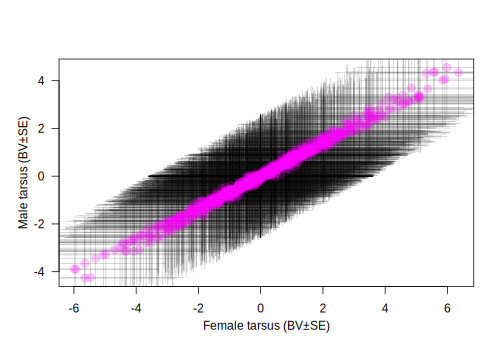
\includegraphics{wam_tuto_files/figure-latex/unnamed-chunk-111-1.pdf} 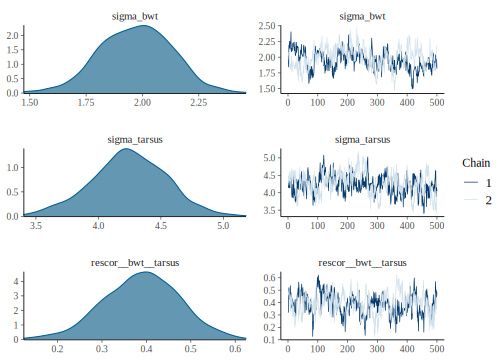
\includegraphics{wam_tuto_files/figure-latex/unnamed-chunk-111-2.pdf}

\begin{Shaded}
\begin{Highlighting}[]
\KeywordTok{VarCorr}\NormalTok{(brms\_m2}\FloatTok{.1}\NormalTok{)}
\end{Highlighting}
\end{Shaded}

\begin{verbatim}
## $animal
## $animal$sd
##                  Estimate Est.Error     Q2.5    Q97.5
## bwt_Intercept    1.808171 0.2050233 1.412824 2.204805
## tarsus_Intercept 3.438368 0.4283612 2.491218 4.245264
## 
## $animal$cor
## , , bwt_Intercept
## 
##                   Estimate Est.Error       Q2.5     Q97.5
## bwt_Intercept    1.0000000 0.0000000 1.00000000 1.0000000
## tarsus_Intercept 0.3814062 0.1380014 0.07581464 0.6209038
## 
## , , tarsus_Intercept
## 
##                   Estimate Est.Error       Q2.5     Q97.5
## bwt_Intercept    0.3814062 0.1380014 0.07581464 0.6209038
## tarsus_Intercept 1.0000000 0.0000000 1.00000000 1.0000000
## 
## 
## $animal$cov
## , , bwt_Intercept
## 
##                  Estimate Est.Error      Q2.5    Q97.5
## bwt_Intercept    3.311473 0.7430185 1.9960721 4.861167
## tarsus_Intercept 2.440166 1.0901689 0.3870783 4.668720
## 
## , , tarsus_Intercept
## 
##                   Estimate Est.Error      Q2.5    Q97.5
## bwt_Intercept     2.440166  1.090169 0.3870783  4.66872
## tarsus_Intercept 12.005688  2.918741 6.2061701 18.02226
## 
## 
## 
## $residual__
## $residual__$sd
##        Estimate Est.Error     Q2.5    Q97.5
## bwt    1.970532 0.1597581 1.658782 2.276074
## tarsus 4.244704 0.2984518 3.632824 4.820109
## 
## $residual__$cor
## , , bwt
## 
##         Estimate  Est.Error      Q2.5     Q97.5
## bwt    1.0000000 0.00000000 1.0000000 1.0000000
## tarsus 0.3888754 0.08510488 0.2127907 0.5526631
## 
## , , tarsus
## 
##         Estimate  Est.Error      Q2.5     Q97.5
## bwt    0.3888754 0.08510488 0.2127907 0.5526631
## tarsus 1.0000000 0.00000000 1.0000000 1.0000000
## 
## 
## $residual__$cov
## , , bwt
## 
##        Estimate Est.Error     Q2.5    Q97.5
## bwt    3.908493 0.6282892 2.751557 5.180511
## tarsus 3.289995 0.9305960 1.572647 5.147133
## 
## , , tarsus
## 
##         Estimate Est.Error      Q2.5     Q97.5
## bwt     3.289995  0.930596  1.572647  5.147133
## tarsus 18.106495  2.530138 13.197409 23.233452
\end{verbatim}

\hypertarget{stan-1}{%
\section{stan}\label{stan-1}}

to do

\hypertarget{rep_measures}{%
\chapter{A repeated measures animal model}\label{rep_measures}}

This tutorial will demonstrate how to run a univariate animal model for a trait with repeated observations using different R packages with an example data files provided.

\hypertarget{scenario-and-data-2}{%
\section{Scenario and data}\label{scenario-and-data-2}}

\hypertarget{scenario-2}{%
\subsection{scenario}\label{scenario-2}}

Since gryphons are iteroparous, multiple observations of reproductive traits are available for some individuals. Here we have repeated measures of lay date (measured in days after January 1) for individual females varying in age from 2 (age of sexual maturation) up until age 6. Not all females lay every year so the number of observations per female is variable (between 1 to 5). We want to know how repeatable the trait is, and (assuming it is repeatable) how heritable it is.

\hypertarget{data-files-2}{%
\subsection{Data files}\label{data-files-2}}

The pedigree file \texttt{gryphonped.csv} is that used in the preceding tutorials but we now use a new data file \texttt{gryphonRM.csv}. Columns correspond to individual identity (\texttt{animal}), birth year (\texttt{byear}), age in years (\texttt{age}), year of measurement (\texttt{year}) and lay date (\texttt{laydate}).
Each row of the data file corresponds to a single phenotypic observation. Here the data is sorted by identity and then age so that the repeated observations on individuals are apparent. However this is not a requirement for analysis - data could equally be sorted by some other variable (\emph{e.g.}, measurement year) or be in a random order.

\begin{Shaded}
\begin{Highlighting}[]
\KeywordTok{str}\NormalTok{(gryphonRM)}
\end{Highlighting}
\end{Shaded}

\begin{verbatim}
## 'data.frame':    1607 obs. of  5 variables:
##  $ animal : Factor w/ 469 levels "1","2","3","8",..: 1 1 1 1 1 2 2 2 3 3 ...
##  $ byear  : Factor w/ 34 levels "968","970","971",..: 22 22 22 22 22 22 22 22 22 22 ...
##  $ age    : Factor w/ 5 levels "2","3","4","5",..: 1 2 3 4 5 1 2 3 1 2 ...
##  $ year   : Factor w/ 39 levels "970","971","972",..: 23 24 25 26 27 23 24 25 23 24 ...
##  $ laydate: num  19 23 24 23 29 21 17 21 20 20 ...
\end{verbatim}

\begin{Shaded}
\begin{Highlighting}[]
\KeywordTok{summary}\NormalTok{(gryphonRM)}
\end{Highlighting}
\end{Shaded}

\begin{verbatim}
##      animal         byear      age          year         laydate     
##  1      :   5   1000   : 109   2:308   1004   :  79   Min.   : 0.00  
##  3      :   5   1001   :  98   3:322   1005   :  78   1st Qu.:20.00  
##  9      :   5   999    :  86   4:339   1003   :  69   Median :24.00  
##  17     :   5   1002   :  85   5:315   1006   :  64   Mean   :23.54  
##  42     :   5   987    :  70   6:323   1002   :  60   3rd Qu.:27.00  
##  50     :   5   989    :  66           988    :  54   Max.   :41.00  
##  (Other):1577   (Other):1093           (Other):1203
\end{verbatim}

\begin{Shaded}
\begin{Highlighting}[]
\KeywordTok{head}\NormalTok{(gryphonRM)}
\end{Highlighting}
\end{Shaded}

\begin{verbatim}
##   animal byear age year laydate
## 1      1   990   2  992      19
## 2      1   990   3  993      23
## 3      1   990   4  994      24
## 4      1   990   5  995      23
## 5      1   990   6  996      29
## 6      2   990   2  992      21
\end{verbatim}

\hypertarget{asreml-r-2}{%
\section{Asreml-R}\label{asreml-r-2}}

\hypertarget{estimating-repeatability}{%
\subsection{Estimating repeatability}\label{estimating-repeatability}}

With repeated measures on individuals it is often of interest to see how repeatable a trait is.
We can estimate the repeatability of a trait as the proportion of phenotypic variance \(V_P\) explained by individual variance \(V_{ind}\); \(R = V_{ind}/V_P = V_{ind}/(V_{ind}+V_R)\).

\begin{Shaded}
\begin{Highlighting}[]
\NormalTok{modelv \textless{}{-}}\StringTok{ }\KeywordTok{asreml}\NormalTok{(}
  \DataTypeTok{fixed =}\NormalTok{ laydate }\OperatorTok{\textasciitilde{}}\StringTok{ }\DecValTok{1}\NormalTok{,}
  \DataTypeTok{random =} \OperatorTok{\textasciitilde{}}\NormalTok{animal,}
  \DataTypeTok{residual =} \OperatorTok{\textasciitilde{}}\StringTok{ }\KeywordTok{idv}\NormalTok{(units),}
  \DataTypeTok{data =}\NormalTok{ gryphonRM,}
  \DataTypeTok{na.action =} \KeywordTok{na.method}\NormalTok{(}\DataTypeTok{x =} \StringTok{"omit"}\NormalTok{, }\DataTypeTok{y =} \StringTok{"omit"}\NormalTok{)}
\NormalTok{)}
\end{Highlighting}
\end{Shaded}

\begin{verbatim}
## Model fitted using the sigma parameterization.
## ASReml 4.1.0 Tue Nov 23 22:11:11 2021
##           LogLik        Sigma2     DF     wall    cpu
##  1     -10182.83           1.0   1606 22:11:11    0.0
##  2      -8266.10           1.0   1606 22:11:11    0.0
##  3      -6145.01           1.0   1606 22:11:11    0.0
##  4      -4651.57           1.0   1606 22:11:11    0.0
##  5      -3819.31           1.0   1606 22:11:11    0.0
##  6      -3554.22           1.0   1606 22:11:11    0.0
##  7      -3501.56           1.0   1606 22:11:11    0.0
##  8      -3497.58           1.0   1606 22:11:11    0.0
##  9      -3497.54           1.0   1606 22:11:11    0.0
## 10      -3497.54           1.0   1606 22:11:11    0.0
\end{verbatim}

\begin{Shaded}
\begin{Highlighting}[]
\KeywordTok{plot}\NormalTok{(modelv)}
\end{Highlighting}
\end{Shaded}

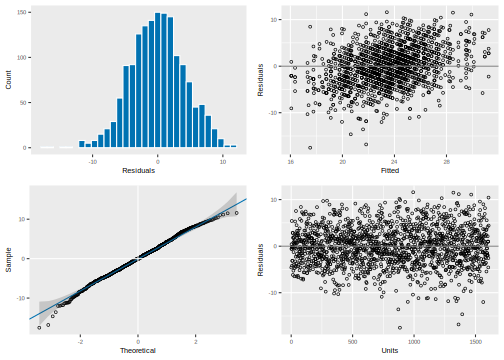
\includegraphics{wam_tuto_files/figure-latex/unnamed-chunk-114-1.pdf}
The model assumption seems correct, so we can look at the different estimates.
Note that since we want to estimate the amount of variance explained by individual identity (rather than by additive genetic effects), we fit \texttt{animal} as a normal random effect and we don't associate it with the pedigree.
Here, we also ask the model to remove any \texttt{NA} in \texttt{laydate}.

This model partitions the phenotypic variance in \texttt{laydate} as follows:

\begin{Shaded}
\begin{Highlighting}[]
\KeywordTok{summary}\NormalTok{(modelv)}\OperatorTok{$}\NormalTok{varcomp}
\end{Highlighting}
\end{Shaded}

\begin{verbatim}
##             component std.error   z.ratio bound %ch
## animal       11.08634 1.1794319  9.399728     P   0
## units!units  21.29643 0.8896196 23.938798     P   0
## units!R       1.00000        NA        NA     F   0
\end{verbatim}

Between-individual (or among-individual) variance is given by the \texttt{animal} component, while the residual component (\texttt{units!units}) represents within-individual variance. Here then the repeatability of the trait can be determined by hand as 0.34 (\emph{i.e.}, as 11.086/(11.086 + 21.296)).

Mean lay date might change with age, so we could ask what the repeatability of lay date is after conditioning on age. This would be done by adding \texttt{age} into the model as a fixed effect.

\begin{Shaded}
\begin{Highlighting}[]
\NormalTok{modelw \textless{}{-}}\StringTok{ }\KeywordTok{asreml}\NormalTok{(}
  \DataTypeTok{fixed =}\NormalTok{ laydate }\OperatorTok{\textasciitilde{}}\StringTok{ }\NormalTok{age,}
  \DataTypeTok{random =} \OperatorTok{\textasciitilde{}}\NormalTok{animal,}
  \DataTypeTok{residual =} \OperatorTok{\textasciitilde{}}\StringTok{ }\KeywordTok{idv}\NormalTok{(units),}
  \DataTypeTok{data =}\NormalTok{ gryphonRM,}
  \DataTypeTok{na.action =} \KeywordTok{na.method}\NormalTok{(}\DataTypeTok{x =} \StringTok{"omit"}\NormalTok{, }\DataTypeTok{y =} \StringTok{"omit"}\NormalTok{)}
\NormalTok{)}
\end{Highlighting}
\end{Shaded}

\begin{verbatim}
## Model fitted using the sigma parameterization.
## ASReml 4.1.0 Tue Nov 23 22:11:13 2021
##           LogLik        Sigma2     DF     wall    cpu
##  1     -8402.968           1.0   1602 22:11:13    0.0
##  2     -6912.361           1.0   1602 22:11:13    0.0
##  3     -5274.379           1.0   1602 22:11:13    0.0
##  4     -4143.634           1.0   1602 22:11:13    0.0
##  5     -3541.895           1.0   1602 22:11:13    0.0
##  6     -3372.909           1.0   1602 22:11:13    0.0
##  7     -3347.670           1.0   1602 22:11:13    0.0
##  8     -3346.655           1.0   1602 22:11:13    0.0
##  9     -3346.652           1.0   1602 22:11:13    0.0
\end{verbatim}

\begin{Shaded}
\begin{Highlighting}[]
\KeywordTok{summary}\NormalTok{(modelw)}\OperatorTok{$}\NormalTok{varcomp}
\end{Highlighting}
\end{Shaded}

\begin{verbatim}
##             component std.error  z.ratio bound %ch
## animal       12.28982  1.156115 10.63027     P   0
## units!units  16.37989  0.686619 23.85586     P   0
## units!R       1.00000        NA       NA     F   0
\end{verbatim}

The repeatability of lay date, after accounting for age effects, is now estimated as 0.43 (\emph{i.e.}, as 12.29/(12.29 + 16.38)).
So, just as we saw when estimating \(h^2\) in Tutorial 1, the inclusion of fixed effects will alter the estimated effect size if we determine total phenotypic variance as the sum of the variance components. Thus, proper interpretation is vital.

\begin{Shaded}
\begin{Highlighting}[]
\KeywordTok{summary}\NormalTok{(modelw, }\DataTypeTok{coef =} \OtherTok{TRUE}\NormalTok{)}\OperatorTok{$}\NormalTok{coef.fixed}
\end{Highlighting}
\end{Shaded}

\begin{verbatim}
##              solution std error   z.ratio
## age_2        0.000000        NA        NA
## age_3        2.577777 0.3355253  7.682811
## age_4        4.247276 0.3309028 12.835418
## age_5        6.094490 0.3375537 18.054872
## age_6        3.132675 0.3371074  9.292811
## (Intercept) 20.305073 0.2899515 70.029214
\end{verbatim}

\begin{Shaded}
\begin{Highlighting}[]
\KeywordTok{wald.asreml}\NormalTok{(modelw, }\DataTypeTok{ssType =} \StringTok{"conditional"}\NormalTok{, }\DataTypeTok{denDF =} \StringTok{"numeric"}\NormalTok{)}
\end{Highlighting}
\end{Shaded}

\begin{verbatim}
## Model fitted using the sigma parameterization.
## ASReml 4.1.0 Tue Nov 23 22:11:13 2021
##           LogLik        Sigma2     DF     wall    cpu
##  1     -3346.652           1.0   1602 22:11:13    0.0
##  2     -3346.652           1.0   1602 22:11:13    0.0
##  3     -3346.652           1.0   1602 22:11:13    0.0
\end{verbatim}

\begin{verbatim}
## $Wald
## 
## Wald tests for fixed effects.
## Response: laydate
## 
##             Df  denDF   F.inc   F.con Margin          Pr
## (Intercept)  1  460.2 14880.0 14880.0        0.00000e+00
## age          4 1225.3    88.7    88.7      A 2.89474e-66
## 
## $stratumVariances
##                    df Variance  animal units!units
## animal       463.8399 56.46460 3.26162           1
## units!units 1138.1601 16.37989 0.00000           1
\end{verbatim}

Here age is modeled as a 5-level factor (specified using the function \texttt{as.factor()} at the beginning of the analysis). We could equally have fitted it as a continuous variable, in which case, given potential for a late life decline, we would probably also include a quadratic term.
In addition, using \texttt{age} as continuous variable can help in saving some degree of freedom in the analysis.

\hypertarget{partitioning-additive-and-permanent-environment-effects}{%
\subsection{Partitioning additive and permanent environment effects}\label{partitioning-additive-and-permanent-environment-effects}}

Generally we expect that the repeatability will set the upper limit for heritability since among individual variation can be decomposed in the additive genetic variation and non additive genetic variation. In other word, the additive genetic variation is a subcomponent of the difference between individuals.
Non-additive contributions to fixed among-individual differences are normally referred to as \emph{permanent environment effects}. If a trait has repeated measures then it is necessary to model permanent environment effects in an animal model to prevent upward bias in \(V_A\).

To illustrate it, we first fit the animal model:

\begin{Shaded}
\begin{Highlighting}[]
\NormalTok{ainv \textless{}{-}}\StringTok{ }\KeywordTok{ainverse}\NormalTok{(gryphonped)}

\NormalTok{modelx \textless{}{-}}\StringTok{ }\KeywordTok{asreml}\NormalTok{(}
  \DataTypeTok{fixed =}\NormalTok{ laydate }\OperatorTok{\textasciitilde{}}\StringTok{ }\NormalTok{age,}
  \DataTypeTok{random =} \OperatorTok{\textasciitilde{}}\StringTok{ }\KeywordTok{vm}\NormalTok{(animal, ainv),}
  \DataTypeTok{residual =} \OperatorTok{\textasciitilde{}}\StringTok{ }\KeywordTok{idv}\NormalTok{(units),}
  \DataTypeTok{data =}\NormalTok{ gryphonRM,}
  \DataTypeTok{na.action =} \KeywordTok{na.method}\NormalTok{(}\DataTypeTok{x =} \StringTok{"omit"}\NormalTok{, }\DataTypeTok{y =} \StringTok{"omit"}\NormalTok{)}
\NormalTok{)}
\end{Highlighting}
\end{Shaded}

\begin{verbatim}
## Model fitted using the sigma parameterization.
## ASReml 4.1.0 Tue Nov 23 22:11:13 2021
##           LogLik        Sigma2     DF     wall    cpu
##  1     -8751.390           1.0   1602 22:11:13    0.0
##  2     -7169.205           1.0   1602 22:11:13    0.0
##  3     -5427.604           1.0   1602 22:11:13    0.0
##  4     -4219.598           1.0   1602 22:11:13    0.0
##  5     -3569.815           1.0   1602 22:11:13    0.0
##  6     -3382.341           1.0   1602 22:11:13    0.0
##  7     -3352.867           1.0   1602 22:11:13    0.0
##  8     -3351.565           1.0   1602 22:11:13    0.0
##  9     -3351.560           1.0   1602 22:11:13    0.0
\end{verbatim}

Variance components are almost unchanged if we compare the previous model:

\begin{Shaded}
\begin{Highlighting}[]
\KeywordTok{summary}\NormalTok{(modelx)}\OperatorTok{$}\NormalTok{varcomp}
\end{Highlighting}
\end{Shaded}

\begin{verbatim}
##                  component std.error   z.ratio bound %ch
## vm(animal, ainv)  13.91784  1.443968  9.638607     P   0
## units!units       16.84008  0.707365 23.806768     P   0
## units!R            1.00000        NA        NA     F   0
\end{verbatim}

\begin{Shaded}
\begin{Highlighting}[]
\KeywordTok{summary}\NormalTok{(modelw)}\OperatorTok{$}\NormalTok{varcomp}
\end{Highlighting}
\end{Shaded}

\begin{verbatim}
##             component std.error  z.ratio bound %ch
## animal       12.28982  1.156115 10.63027     P   0
## units!units  16.37989  0.686619 23.85586     P   0
## units!R       1.00000        NA       NA     F   0
\end{verbatim}

This suggests that most of the among-individual variance is -- rightly or wrongly -- being partitioned as \(V_A\) here. To instead to obtain an unbiased estimate of \(V_A\), we need to partition for both additive genetic \emph{and} non-genetic sources of individual variation. We do it by fitting \texttt{animal} twice, once with a pedigree, and once without a pedigree (using \texttt{ide()}).
Here, the command \texttt{ide} allow to create a second effect using a similar variable.

\begin{Shaded}
\begin{Highlighting}[]
\NormalTok{modely \textless{}{-}}\StringTok{ }\KeywordTok{asreml}\NormalTok{(}
  \DataTypeTok{fixed =}\NormalTok{ laydate }\OperatorTok{\textasciitilde{}}\StringTok{ }\NormalTok{age,}
  \DataTypeTok{random =} \OperatorTok{\textasciitilde{}}\StringTok{ }\KeywordTok{vm}\NormalTok{(animal, ainv) }\OperatorTok{+}\StringTok{ }\KeywordTok{ide}\NormalTok{(animal),}
  \DataTypeTok{residual =} \OperatorTok{\textasciitilde{}}\StringTok{ }\KeywordTok{idv}\NormalTok{(units),}
  \DataTypeTok{data =}\NormalTok{ gryphonRM,}
  \DataTypeTok{na.action =} \KeywordTok{na.method}\NormalTok{(}\DataTypeTok{x =} \StringTok{"omit"}\NormalTok{, }\DataTypeTok{y =} \StringTok{"omit"}\NormalTok{)}
\NormalTok{)}
\end{Highlighting}
\end{Shaded}

\begin{verbatim}
## Model fitted using the sigma parameterization.
## ASReml 4.1.0 Tue Nov 23 22:11:13 2021
##           LogLik        Sigma2     DF     wall    cpu
##  1     -7731.394           1.0   1602 22:11:13    0.0
##  2     -6426.548           1.0   1602 22:11:13    0.0
##  3     -4997.252           1.0   1602 22:11:13    0.0
##  4     -4018.486           1.0   1602 22:11:13    0.0
##  5     -3504.988           1.0   1602 22:11:13    0.0
##  6     -3363.160           1.0   1602 22:11:13    0.0
##  7     -3341.611           1.0   1602 22:11:13    0.0
##  8     -3340.682           1.0   1602 22:11:13    0.0
##  9     -3340.679           1.0   1602 22:11:13    0.0
\end{verbatim}

\begin{Shaded}
\begin{Highlighting}[]
\KeywordTok{summary}\NormalTok{(modely)}\OperatorTok{$}\NormalTok{varcomp}
\end{Highlighting}
\end{Shaded}

\begin{verbatim}
##                  component std.error   z.ratio bound %ch
## vm(animal, ainv)  4.876101 1.8087709  2.695809     P   0
## ide(animal)       7.400983 1.7280113  4.282948     P   0
## units!units      16.380188 0.6866189 23.856300     P   0
## units!R           1.000000        NA        NA     F   0
\end{verbatim}

The estimate of \(V_A\) is now much lower since the additive and permanent environment effects are being properly separated. We can estimate \(h^2\) and the repeatability from this model:

\begin{Shaded}
\begin{Highlighting}[]
\KeywordTok{vpredict}\NormalTok{(modely, h2 }\OperatorTok{\textasciitilde{}}\StringTok{ }\NormalTok{V1 }\OperatorTok{/}\StringTok{ }\NormalTok{(V1 }\OperatorTok{+}\StringTok{ }\NormalTok{V2 }\OperatorTok{+}\StringTok{ }\NormalTok{V3))}
\end{Highlighting}
\end{Shaded}

\begin{verbatim}
##     Estimate         SE
## h2 0.1701523 0.06073974
\end{verbatim}

\begin{Shaded}
\begin{Highlighting}[]
\KeywordTok{vpredict}\NormalTok{(modely, repeatability }\OperatorTok{\textasciitilde{}}\StringTok{ }\NormalTok{(V1 }\OperatorTok{+}\StringTok{ }\NormalTok{V2) }\OperatorTok{/}\StringTok{ }\NormalTok{(V1 }\OperatorTok{+}\StringTok{ }\NormalTok{V2 }\OperatorTok{+}\StringTok{ }\NormalTok{V3))}
\end{Highlighting}
\end{Shaded}

\begin{verbatim}
##                Estimate         SE
## repeatability 0.4284108 0.02741602
\end{verbatim}

\hypertarget{adding-additional-effects-and-testing-significance}{%
\subsection{Adding additional effects and testing significance}\label{adding-additional-effects-and-testing-significance}}

Models of repeated measures can be extended to include other fixed or random effects. For example try including year of measurement (\texttt{year}) and birth year (\texttt{byear}) as random effects.

\begin{Shaded}
\begin{Highlighting}[]
\NormalTok{modelz \textless{}{-}}\StringTok{ }\KeywordTok{asreml}\NormalTok{(}
  \DataTypeTok{fixed =}\NormalTok{ laydate }\OperatorTok{\textasciitilde{}}\StringTok{ }\NormalTok{age,}
  \DataTypeTok{random =} \OperatorTok{\textasciitilde{}}\StringTok{ }\KeywordTok{vm}\NormalTok{(animal, ainv) }\OperatorTok{+}\StringTok{ }\KeywordTok{ide}\NormalTok{(animal) }\OperatorTok{+}
\StringTok{    }\NormalTok{year }\OperatorTok{+}\StringTok{ }\NormalTok{byear,}
  \DataTypeTok{residual =} \OperatorTok{\textasciitilde{}}\StringTok{ }\KeywordTok{idv}\NormalTok{(units),}
  \DataTypeTok{data =}\NormalTok{ gryphonRM,}
  \DataTypeTok{na.action =} \KeywordTok{na.method}\NormalTok{(}\DataTypeTok{x =} \StringTok{"omit"}\NormalTok{, }\DataTypeTok{y =} \StringTok{"omit"}\NormalTok{)}
\NormalTok{)}
\end{Highlighting}
\end{Shaded}

\begin{verbatim}
## Model fitted using the sigma parameterization.
## ASReml 4.1.0 Tue Nov 23 22:11:13 2021
##           LogLik        Sigma2     DF     wall    cpu
##  1     -4650.748           1.0   1602 22:11:13    0.0
##  2     -4088.264           1.0   1602 22:11:13    0.0
##  3     -3494.147           1.0   1602 22:11:13    0.0
##  4     -3127.161           1.0   1602 22:11:13    0.0 (1 restrained)
##  5     -2976.449           1.0   1602 22:11:13    0.0 (1 restrained)
##  6     -2955.785           1.0   1602 22:11:13    0.0 (1 restrained)
##  7     -2955.097           1.0   1602 22:11:13    0.0 (1 restrained)
##  8     -2955.095           1.0   1602 22:11:13    0.0 (1 restrained)
##  9     -2955.095           1.0   1602 22:11:13    0.0
\end{verbatim}

\begin{Shaded}
\begin{Highlighting}[]
\KeywordTok{summary}\NormalTok{(modelz)}\OperatorTok{$}\NormalTok{varcomp}
\end{Highlighting}
\end{Shaded}

\begin{verbatim}
##                     component std.error   z.ratio bound %ch
## byear            1.650876e-07        NA        NA     B   0
## year             7.938576e+00 1.9344619  4.103765     P   0
## vm(animal, ainv) 4.815136e+00 1.6682351  2.886365     P   0
## ide(animal)      8.433325e+00 1.5495778  5.442337     P   0
## units!units      7.795560e+00 0.3324411 23.449443     P   0
## units!R          1.000000e+00        NA        NA     F   0
\end{verbatim}

This model will return additional variance components corresponding to variation in lay dates between years of measurement and between birth cohorts of females. \(V_{byear}\) is very low and \texttt{B} appeared which tell us that the model had fixed the variance as a boundary. If you compare this model to a reduced model with byear excluded the log-likelihood remains unchanged.

\begin{Shaded}
\begin{Highlighting}[]
\NormalTok{modelz\_}\DecValTok{2}\NormalTok{ \textless{}{-}}\StringTok{ }\KeywordTok{asreml}\NormalTok{(}
  \DataTypeTok{fixed =}\NormalTok{ laydate }\OperatorTok{\textasciitilde{}}\StringTok{ }\NormalTok{age,}
  \DataTypeTok{random =} \OperatorTok{\textasciitilde{}}\StringTok{ }\KeywordTok{vm}\NormalTok{(animal, ainv) }\OperatorTok{+}\StringTok{ }\KeywordTok{ide}\NormalTok{(animal) }\OperatorTok{+}
\StringTok{    }\NormalTok{year,}
  \DataTypeTok{residual =} \OperatorTok{\textasciitilde{}}\StringTok{ }\KeywordTok{idv}\NormalTok{(units),}
  \DataTypeTok{data =}\NormalTok{ gryphonRM,}
  \DataTypeTok{na.action =} \KeywordTok{na.method}\NormalTok{(}\DataTypeTok{x =} \StringTok{"omit"}\NormalTok{, }\DataTypeTok{y =} \StringTok{"omit"}\NormalTok{)}
\NormalTok{)}
\end{Highlighting}
\end{Shaded}

\begin{verbatim}
## Model fitted using the sigma parameterization.
## ASReml 4.1.0 Tue Nov 23 22:11:13 2021
##           LogLik        Sigma2     DF     wall    cpu
##  1     -4665.606           1.0   1602 22:11:13    0.0
##  2     -4097.928           1.0   1602 22:11:13    0.0
##  3     -3498.611           1.0   1602 22:11:14    0.0
##  4     -3128.789           1.0   1602 22:11:14    0.0
##  5     -2976.883           1.0   1602 22:11:14    0.0
##  6     -2955.806           1.0   1602 22:11:14    0.0
##  7     -2955.096           1.0   1602 22:11:14    0.0
##  8     -2955.095           1.0   1602 22:11:14    0.0
\end{verbatim}

\begin{Shaded}
\begin{Highlighting}[]
\KeywordTok{summary}\NormalTok{(modelz\_}\DecValTok{2}\NormalTok{)}\OperatorTok{$}\NormalTok{varcomp}
\end{Highlighting}
\end{Shaded}

\begin{verbatim}
##                  component std.error   z.ratio bound %ch
## year              7.938576 1.9344829  4.103720     P   0
## vm(animal, ainv)  4.815137 1.6682366  2.886364     P   0
## ide(animal)       8.433324 1.5495828  5.442319     P   0
## units!units       7.795560 0.3324384 23.449637     P   0
## units!R           1.000000        NA        NA     F   0
\end{verbatim}

\begin{Shaded}
\begin{Highlighting}[]
\NormalTok{modelz}\OperatorTok{$}\NormalTok{loglik}
\end{Highlighting}
\end{Shaded}

\begin{verbatim}
## [1] -2955.095
\end{verbatim}

\begin{Shaded}
\begin{Highlighting}[]
\NormalTok{modelz\_}\DecValTok{2}\OperatorTok{$}\NormalTok{loglik}
\end{Highlighting}
\end{Shaded}

\begin{verbatim}
## [1] -2955.095
\end{verbatim}

\begin{Shaded}
\begin{Highlighting}[]
\DecValTok{1} \OperatorTok{{-}}\StringTok{ }\KeywordTok{pchisq}\NormalTok{(}\DecValTok{2} \OperatorTok{*}\StringTok{ }\NormalTok{(modelz\_}\DecValTok{2}\OperatorTok{$}\NormalTok{loglik }\OperatorTok{{-}}\StringTok{ }\NormalTok{modelz}\OperatorTok{$}\NormalTok{loglik), }\DecValTok{1}\NormalTok{)}
\end{Highlighting}
\end{Shaded}

\begin{verbatim}
## [1] 0.9990425
\end{verbatim}

\texttt{year} effects could alternatively be included as fixed effects (try it!). This will reduce \(V_R\) and increase the estimates of heritability and repeatability, which must now be interpreted as proportions of phenotypic variance after conditioning on both age and year of measurement effects.

\begin{Shaded}
\begin{Highlighting}[]
\NormalTok{modelz\_}\DecValTok{3}\NormalTok{ \textless{}{-}}\StringTok{ }\KeywordTok{asreml}\NormalTok{(}
  \DataTypeTok{fixed =}\NormalTok{ laydate }\OperatorTok{\textasciitilde{}}\StringTok{ }\NormalTok{age}\OperatorTok{+}\NormalTok{byear,}
  \DataTypeTok{random =} \OperatorTok{\textasciitilde{}}\StringTok{ }\KeywordTok{vm}\NormalTok{(animal, ainv) }\OperatorTok{+}\StringTok{ }\KeywordTok{ide}\NormalTok{(animal) }\OperatorTok{+}
\StringTok{    }\NormalTok{year,}
  \DataTypeTok{residual =} \OperatorTok{\textasciitilde{}}\StringTok{ }\KeywordTok{idv}\NormalTok{(units),}
  \DataTypeTok{data =}\NormalTok{ gryphonRM,}
  \DataTypeTok{na.action =} \KeywordTok{na.method}\NormalTok{(}\DataTypeTok{x =} \StringTok{"omit"}\NormalTok{, }\DataTypeTok{y =} \StringTok{"omit"}\NormalTok{)}
\NormalTok{)}
\end{Highlighting}
\end{Shaded}

\begin{verbatim}
## Model fitted using the sigma parameterization.
## ASReml 4.1.0 Tue Nov 23 22:11:14 2021
##           LogLik        Sigma2     DF     wall    cpu
##  1     -4623.985           1.0   1569 22:11:14    0.0
##  2     -4063.535           1.0   1569 22:11:14    0.0
##  3     -3471.618           1.0   1569 22:11:14    0.0
##  4     -3105.972           1.0   1569 22:11:14    0.0
##  5     -2955.436           1.0   1569 22:11:14    0.0
##  6     -2934.435           1.0   1569 22:11:14    0.0
##  7     -2933.721           1.0   1569 22:11:14    0.0
##  8     -2933.720           1.0   1569 22:11:14    0.0
\end{verbatim}

\begin{Shaded}
\begin{Highlighting}[]
\KeywordTok{summary}\NormalTok{(modelz\_}\DecValTok{3}\NormalTok{)}\OperatorTok{$}\NormalTok{varcomp}
\end{Highlighting}
\end{Shaded}

\begin{verbatim}
##                  component std.error   z.ratio bound %ch
## year              8.029139 1.9920127  4.030666     P   0
## vm(animal, ainv)  5.060775 1.7855255  2.834334     P   0
## ide(animal)       8.412539 1.6494894  5.100087     P   0
## units!units       7.805139 0.3331474 23.428484     P   0
## units!R           1.000000        NA        NA     F   0
\end{verbatim}

\begin{Shaded}
\begin{Highlighting}[]
\KeywordTok{wald.asreml}\NormalTok{(modelz\_}\DecValTok{3}\NormalTok{, }\DataTypeTok{ssType =} \StringTok{"conditional"}\NormalTok{, }\DataTypeTok{denDF =} \StringTok{"numeric"}\NormalTok{)}
\end{Highlighting}
\end{Shaded}

\begin{verbatim}
## Model fitted using the sigma parameterization.
\end{verbatim}

\begin{verbatim}
## Warning in asreml(fixed = laydate ~ age + byear, random = ~vm(animal, ainv) + :
## Algebraic derivatives for denominator df not available.
\end{verbatim}

\begin{verbatim}
## ASReml 4.1.0 Tue Nov 23 22:11:14 2021
##           LogLik        Sigma2     DF     wall    cpu
##  1     -2933.720           1.0   1569 22:11:14    0.0
##  2     -2933.720           1.0   1569 22:11:14    0.0
## Calculating denominator DF
\end{verbatim}

\begin{verbatim}
## $Wald
## 
## Wald tests for fixed effects.
## Response: laydate
## 
##             Df denDF   F.inc   F.con Margin      Pr
## (Intercept)  1  55.3 1894.00 1894.00        0.00000
## age          4 845.2  152.70  132.90      A 0.00000
## byear       33 466.5    0.77    0.77      A 0.81646
## 
## $stratumVariances
##                          df  Variance     year vm(animal, ainv) ide(animal)
## year               35.92378 144.92624 17.16741      -0.02687884 -0.06922989
## vm(animal, ainv)  348.27527  50.82831  0.00000       3.50972263  3.00281025
## ide(animal)        87.03390  34.64049  0.00000       0.00000000  3.18992331
## units!units      1097.76705   7.80514  0.00000       0.00000000  0.00000000
##                  units!units
## year                       1
## vm(animal, ainv)           1
## ide(animal)                1
## units!units                1
\end{verbatim}

\hypertarget{gremlin-3}{%
\section{gremlin}\label{gremlin-3}}

TODO (maybe just bother Matthew to do it)

Meanwhile

\begin{figure}

\includegraphics[width=1\linewidth]{images/Gizmo} \caption{Keep it dry and do no feed after midnight.}\label{fig:unnamed-chunk-126}
\end{figure}

\hypertarget{mcmcglmm-3}{%
\section{MCMCglmm}\label{mcmcglmm-3}}

\hypertarget{estimating-repeatability-1}{%
\subsection{Estimating repeatability}\label{estimating-repeatability-1}}

With repeated measures on individuals it is often of interest to see how repeatable a trait is.
We can estimate the repeatability of a trait as the proportion of phenotypic variance \(V_P\) explained by individual variance \(V_{ind}\); \(R = V_{ind}/V_P = V_{ind}/(V_{ind}+V_R)\).
As you already know, bayesian modelisation requires prior. Here, we create a unformative prior with one estimate for the G matrix and one estimate for the Residual matrix, in addition

\begin{Shaded}
\begin{Highlighting}[]
\CommentTok{\#p.var \textless{}{-} var(gryphonRM$laydate, na.rm = TRUE)}
\NormalTok{prior3}\FloatTok{.1}\NormalTok{ \textless{}{-}}\StringTok{ }\KeywordTok{list}\NormalTok{(}\DataTypeTok{G =} \KeywordTok{list}\NormalTok{(}\DataTypeTok{G1 =} \KeywordTok{list}\NormalTok{(}\DataTypeTok{V =} \DecValTok{1}\NormalTok{, }\DataTypeTok{nu =} \FloatTok{0.002}\NormalTok{)), }\DataTypeTok{R =} \KeywordTok{list}\NormalTok{(}
  \DataTypeTok{V =} \DecValTok{1}\NormalTok{,}
  \DataTypeTok{nu =} \FloatTok{0.002}
\NormalTok{))}
\NormalTok{model3}\FloatTok{.1}\NormalTok{ \textless{}{-}}\StringTok{ }\KeywordTok{MCMCglmm}\NormalTok{(laydate }\OperatorTok{\textasciitilde{}}\StringTok{ }\DecValTok{1}\NormalTok{,}
  \DataTypeTok{random =} \OperatorTok{\textasciitilde{}}\NormalTok{animal, }\DataTypeTok{data =}\NormalTok{ gryphonRM,}
  \DataTypeTok{prior =}\NormalTok{ prior3}\FloatTok{.1}\NormalTok{, }\DataTypeTok{verbose =} \OtherTok{FALSE}
\NormalTok{)}
\KeywordTok{posterior.mode}\NormalTok{(model3}\FloatTok{.1}\OperatorTok{$}\NormalTok{VCV)}
\end{Highlighting}
\end{Shaded}

\begin{verbatim}
##   animal    units 
## 10.48319 20.89898
\end{verbatim}

Note the use of the term \texttt{animal} as random allowed to partition the phenotypic variance \(V_P\) into among individual variance \(V_{ind}\) associated with \texttt{animal} and residual variance \(V_R\) associated with \texttt{units}.

Here then the repeatability of the \texttt{laydate} can be determined as: 21.9 (\emph{i.e.}, as 10.483/(10.483 + 20.899)). Just a friendly remember, we work with Monte Carlo chain with model iteration, so the point estimate can be different (but very similar) each time you run the model.

Mean lay date might change with age, so we could ask what the repeatability of lay date is after conditioning on age. This would be done by adding \texttt{age} into the model as a fixed effect.

\begin{Shaded}
\begin{Highlighting}[]
\NormalTok{model3}\FloatTok{.2}\NormalTok{ \textless{}{-}}\StringTok{ }\KeywordTok{MCMCglmm}\NormalTok{(laydate }\OperatorTok{\textasciitilde{}}\StringTok{ }\NormalTok{age,}
  \DataTypeTok{random =} \OperatorTok{\textasciitilde{}}\NormalTok{animal, }\DataTypeTok{data =}\NormalTok{ gryphonRM,}
  \DataTypeTok{prior =}\NormalTok{ prior3}\FloatTok{.1}\NormalTok{, }\DataTypeTok{verbose =} \OtherTok{FALSE}
\NormalTok{)}
\KeywordTok{plot}\NormalTok{(model3}\FloatTok{.2}\OperatorTok{$}\NormalTok{Sol)}
\end{Highlighting}
\end{Shaded}

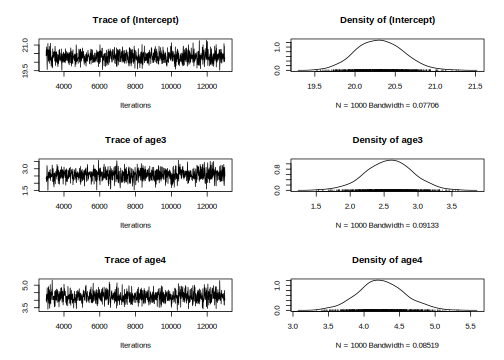
\includegraphics{wam_tuto_files/figure-latex/unnamed-chunk-128-1.pdf} 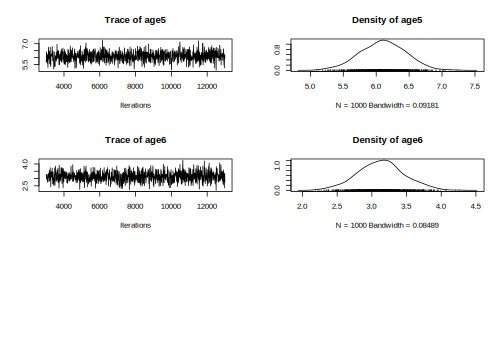
\includegraphics{wam_tuto_files/figure-latex/unnamed-chunk-128-2.pdf}

\begin{Shaded}
\begin{Highlighting}[]
\KeywordTok{plot}\NormalTok{(model3}\FloatTok{.2}\OperatorTok{$}\NormalTok{VCV)}
\end{Highlighting}
\end{Shaded}

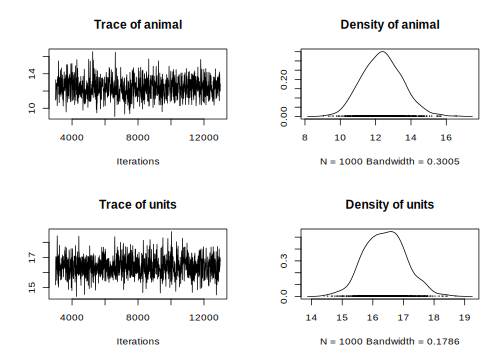
\includegraphics{wam_tuto_files/figure-latex/unnamed-chunk-128-3.pdf}

\begin{Shaded}
\begin{Highlighting}[]
\KeywordTok{posterior.mode}\NormalTok{(model3}\FloatTok{.2}\OperatorTok{$}\NormalTok{VCV)}
\end{Highlighting}
\end{Shaded}

\begin{verbatim}
##   animal    units 
## 12.04167 16.60341
\end{verbatim}

The model assumption seems correct, so we can look at the different estimates.
Note that the random effect structure has remained unchanged because we did not modified the prior \texttt{prior3.1}.
The repeatability of \texttt{laydate}, after accounting for age effects, is now estimated as21.9 (\emph{i.e.}, as 10.483/(10.483 + 20.899)).
Just as we saw when estimating \(h_2\) in tutorial 1, the inclusion of fixed effects will alter the estimated effect size if we determine total phenotypic variance as the sum of the variance components. Thus, proper interpretation is vital.

\begin{Shaded}
\begin{Highlighting}[]
\KeywordTok{plot}\NormalTok{(model3}\FloatTok{.2}\OperatorTok{$}\NormalTok{Sol)}
\end{Highlighting}
\end{Shaded}

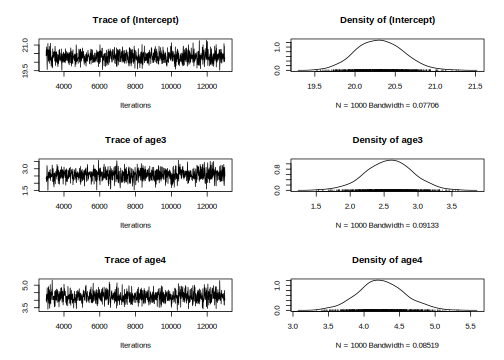
\includegraphics{wam_tuto_files/figure-latex/unnamed-chunk-129-1.pdf} 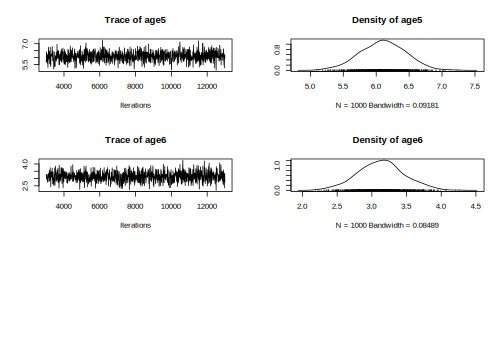
\includegraphics{wam_tuto_files/figure-latex/unnamed-chunk-129-2.pdf}

\begin{Shaded}
\begin{Highlighting}[]
\KeywordTok{posterior.mode}\NormalTok{(model3}\FloatTok{.2}\OperatorTok{$}\NormalTok{Sol)}
\end{Highlighting}
\end{Shaded}

\begin{verbatim}
## (Intercept)        age3        age4        age5        age6 
##   20.427701    2.487962    4.155696    6.122910    3.204512
\end{verbatim}

\begin{Shaded}
\begin{Highlighting}[]
\KeywordTok{HPDinterval}\NormalTok{(model3}\FloatTok{.2}\OperatorTok{$}\NormalTok{Sol, }\FloatTok{0.95}\NormalTok{)}
\end{Highlighting}
\end{Shaded}

\begin{verbatim}
##                 lower     upper
## (Intercept) 19.739184 20.888281
## age3         1.908402  3.250027
## age4         3.641353  4.978971
## age5         5.456836  6.759925
## age6         2.480376  3.818013
## attr(,"Probability")
## [1] 0.95
\end{verbatim}

Here age is modeled as a 5-level factor (specified using the function \texttt{as.factor()} at the beginning of the analysis). We could equally have fitted it as a continuous variable, in which case, given potential for a late life decline, we would probably also include a quadratic term.
In addition, using \texttt{age} as continuous variable can help in saving some degree of freedom in the analysis.

\begin{Shaded}
\begin{Highlighting}[]
\NormalTok{gryphonRM}\OperatorTok{$}\NormalTok{age\_c \textless{}{-}}\StringTok{ }\KeywordTok{as.numeric}\NormalTok{(gryphonRM}\OperatorTok{$}\NormalTok{age)}

\NormalTok{model3}\FloatTok{.2}\NormalTok{\_}\DecValTok{2}\NormalTok{ \textless{}{-}}\StringTok{ }\KeywordTok{MCMCglmm}\NormalTok{(laydate }\OperatorTok{\textasciitilde{}}\StringTok{ }\NormalTok{age\_c}\OperatorTok{+}\StringTok{ }\KeywordTok{I}\NormalTok{(age\_c}\OperatorTok{\^{}}\DecValTok{2}\NormalTok{),}
  \DataTypeTok{random =} \OperatorTok{\textasciitilde{}}\NormalTok{animal, }\DataTypeTok{data =}\NormalTok{ gryphonRM,}
  \DataTypeTok{prior =}\NormalTok{ prior3}\FloatTok{.1}\NormalTok{, }\DataTypeTok{verbose =} \OtherTok{FALSE}
\NormalTok{)}
\KeywordTok{plot}\NormalTok{(model3}\FloatTok{.2}\NormalTok{\_}\DecValTok{2}\OperatorTok{$}\NormalTok{Sol)}
\end{Highlighting}
\end{Shaded}

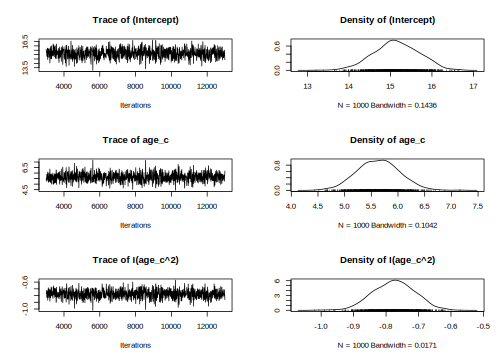
\includegraphics{wam_tuto_files/figure-latex/unnamed-chunk-130-1.pdf}

\begin{Shaded}
\begin{Highlighting}[]
\KeywordTok{plot}\NormalTok{(model3}\FloatTok{.2}\NormalTok{\_}\DecValTok{2}\OperatorTok{$}\NormalTok{VCV)}
\end{Highlighting}
\end{Shaded}

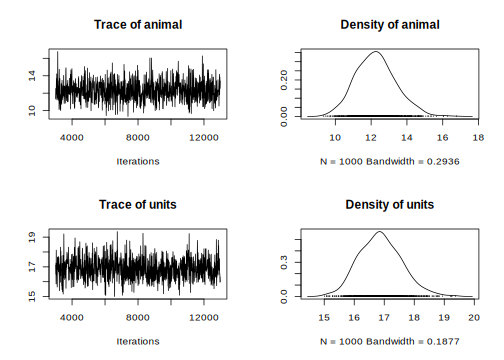
\includegraphics{wam_tuto_files/figure-latex/unnamed-chunk-130-2.pdf}

\begin{Shaded}
\begin{Highlighting}[]
\KeywordTok{posterior.mode}\NormalTok{(model3}\FloatTok{.2}\NormalTok{\_}\DecValTok{2}\OperatorTok{$}\NormalTok{VCV)}
\end{Highlighting}
\end{Shaded}

\begin{verbatim}
##   animal    units 
## 12.67652 16.87004
\end{verbatim}

\begin{Shaded}
\begin{Highlighting}[]
\KeywordTok{posterior.mode}\NormalTok{(model3}\FloatTok{.2}\NormalTok{\_}\DecValTok{2}\OperatorTok{$}\NormalTok{Sol)}
\end{Highlighting}
\end{Shaded}

\begin{verbatim}
## (Intercept)       age_c  I(age_c^2) 
##  14.9865627   5.5782580  -0.7797179
\end{verbatim}

\begin{Shaded}
\begin{Highlighting}[]
\KeywordTok{HPDinterval}\NormalTok{(model3}\FloatTok{.2}\NormalTok{\_}\DecValTok{2}\OperatorTok{$}\NormalTok{Sol, }\FloatTok{0.95}\NormalTok{)}
\end{Highlighting}
\end{Shaded}

\begin{verbatim}
##                  lower      upper
## (Intercept) 13.8649578 16.0180520
## age_c        4.7944293  6.4030085
## I(age_c^2)  -0.9120611 -0.6511249
## attr(,"Probability")
## [1] 0.95
\end{verbatim}

\hypertarget{partitioning-additive-and-permanent-environment-effects-1}{%
\subsection{Partitioning additive and permanent environment effects}\label{partitioning-additive-and-permanent-environment-effects-1}}

Generally we expect that the repeatability will set the upper limit for heritability since among individual variation can be decomposed in the additive genetic variation and non additive genetic variation. In other word, the additive genetic variation is a subcomponent of the difference between individuals.
Non-additive contributions to fixed among-individual differences are normally referred to as \emph{permanent environment effects}. If a trait has repeated measures then it is necessary to model permanent environment effects in an animal model to prevent upward bias in \(V_A\).

To illustrate it, we first fit the animal model:

\begin{Shaded}
\begin{Highlighting}[]
\NormalTok{Ainv \textless{}{-}}\StringTok{ }\KeywordTok{inverseA}\NormalTok{(gryphonped)}\OperatorTok{$}\NormalTok{Ainv}
\NormalTok{model3}\FloatTok{.3}\NormalTok{ \textless{}{-}}\StringTok{ }\KeywordTok{MCMCglmm}\NormalTok{(laydate }\OperatorTok{\textasciitilde{}}\StringTok{ }\DecValTok{1} \OperatorTok{+}\StringTok{ }\NormalTok{age,}
  \DataTypeTok{random =} \OperatorTok{\textasciitilde{}}\NormalTok{animal, }\DataTypeTok{ginv =} \KeywordTok{list}\NormalTok{(}\DataTypeTok{animal =}\NormalTok{ Ainv),}
  \DataTypeTok{data =}\NormalTok{ gryphonRM, }\DataTypeTok{prior =}\NormalTok{ prior3}\FloatTok{.1}\NormalTok{, }\DataTypeTok{verbose =} \OtherTok{FALSE}
\NormalTok{)}
\end{Highlighting}
\end{Shaded}

Variance components are almost unchanged if we compare the previous model:

\begin{Shaded}
\begin{Highlighting}[]
\KeywordTok{posterior.mode}\NormalTok{(model3}\FloatTok{.3}\OperatorTok{$}\NormalTok{VCV)}
\end{Highlighting}
\end{Shaded}

\begin{verbatim}
##   animal    units 
## 13.93557 16.83863
\end{verbatim}

\begin{Shaded}
\begin{Highlighting}[]
\KeywordTok{posterior.mode}\NormalTok{(model3}\FloatTok{.2}\OperatorTok{$}\NormalTok{VCV)}
\end{Highlighting}
\end{Shaded}

\begin{verbatim}
##   animal    units 
## 12.04167 16.60341
\end{verbatim}

This suggests that most of the among-individual variance is -- rightly or wrongly -- being partitioned as \(V_A\) here. In fact here the partition is wrong since the simulation included both additive genetic effects and additional fixed heterogeneity that was not associated with the pedigree structure (i.e.~permanent environment effects).
In order to o obtain an unbiased estimate of \(V_A\), we need to fit the individual identity twice in the model: once linked to the pedigree (genetic effect) and once not linked to the pedigree (permanent environment effect).To do so, we need to duplicate the variable containing the individual identity \texttt{animal} and give it a new name. In addition, the prior need to be modified to integrate a seconf random effect.An more appropriate estimate of \(V_A\) is given by the model:

\begin{Shaded}
\begin{Highlighting}[]
\NormalTok{gryphonRM}\OperatorTok{$}\NormalTok{animal\_pe \textless{}{-}}\StringTok{ }\NormalTok{gryphonRM}\OperatorTok{$}\NormalTok{animal}
\CommentTok{\#p.var \textless{}{-} var(gryphonRM$laydate, na.rm = TRUE)}
\NormalTok{prior3}\FloatTok{.4}\NormalTok{ \textless{}{-}}\StringTok{ }\KeywordTok{list}\NormalTok{(}\DataTypeTok{G =} \KeywordTok{list}\NormalTok{(}\DataTypeTok{G1 =} \KeywordTok{list}\NormalTok{(}\DataTypeTok{V =} \DecValTok{1}\NormalTok{, }\DataTypeTok{nu =} \FloatTok{0.002}\NormalTok{), }\DataTypeTok{G2 =} \KeywordTok{list}\NormalTok{(}
  \DataTypeTok{V =} \DecValTok{1}\NormalTok{,}
  \DataTypeTok{nu =} \FloatTok{0.002}
\NormalTok{)), }\DataTypeTok{R =} \KeywordTok{list}\NormalTok{(}\DataTypeTok{V =} \DecValTok{1}\NormalTok{, }\DataTypeTok{nu =} \FloatTok{0.002}\NormalTok{))}
\NormalTok{model3}\FloatTok{.4}\NormalTok{ \textless{}{-}}\StringTok{ }\KeywordTok{MCMCglmm}\NormalTok{(laydate }\OperatorTok{\textasciitilde{}}\StringTok{ }\DecValTok{1} \OperatorTok{+}\StringTok{ }\NormalTok{age,}
  \DataTypeTok{random =} \OperatorTok{\textasciitilde{}}\StringTok{ }\NormalTok{animal }\OperatorTok{+}\StringTok{ }\NormalTok{animal\_pe,}
  \DataTypeTok{ginv =} \KeywordTok{list}\NormalTok{(}\DataTypeTok{animal =}\NormalTok{ Ainv), }\DataTypeTok{data =}\NormalTok{ gryphonRM, }\DataTypeTok{prior =}\NormalTok{ prior3}\FloatTok{.4}\NormalTok{, }\DataTypeTok{verbose =} \OtherTok{FALSE}
\NormalTok{)}
\KeywordTok{posterior.mode}\NormalTok{(model3}\FloatTok{.4}\OperatorTok{$}\NormalTok{VCV)}
\end{Highlighting}
\end{Shaded}

\begin{verbatim}
##    animal animal_pe     units 
##  2.984047  7.026084 16.485572
\end{verbatim}

The estimate of\(V_A\) is now much lower (reduced from 13.6735 to 5.1238) due to a proper separation in the additive and permanent environment effects.
We can estimate \(h^2\) and the repeatability from this model:

\begin{Shaded}
\begin{Highlighting}[]
\NormalTok{model3.}\FloatTok{4.}\NormalTok{VP \textless{}{-}}\StringTok{ }\NormalTok{model3}\FloatTok{.4}\OperatorTok{$}\NormalTok{VCV[, }\StringTok{"animal"}\NormalTok{] }\OperatorTok{+}\StringTok{ }\NormalTok{model3}\FloatTok{.4}\OperatorTok{$}\NormalTok{VCV[, }\StringTok{"animal\_pe"}\NormalTok{] }\OperatorTok{+}\StringTok{ }\NormalTok{model3}\FloatTok{.4}\OperatorTok{$}\NormalTok{VCV[, }\StringTok{"units"}\NormalTok{]}
\NormalTok{model3.}\FloatTok{4.}\NormalTok{PE\_VA \textless{}{-}}\StringTok{ }\NormalTok{model3}\FloatTok{.4}\OperatorTok{$}\NormalTok{VCV[, }\StringTok{"animal"}\NormalTok{] }\OperatorTok{+}\StringTok{ }\NormalTok{model3}\FloatTok{.4}\OperatorTok{$}\NormalTok{VCV[, }\StringTok{"animal\_pe"}\NormalTok{]}
\KeywordTok{posterior.mode}\NormalTok{(model3.}\FloatTok{4.}\NormalTok{PE\_VA }\OperatorTok{/}\StringTok{ }\NormalTok{model3.}\FloatTok{4.}\NormalTok{VP)}
\end{Highlighting}
\end{Shaded}

\begin{verbatim}
##     var1 
## 0.414456
\end{verbatim}

\begin{Shaded}
\begin{Highlighting}[]
\KeywordTok{posterior.mode}\NormalTok{(model3}\FloatTok{.4}\OperatorTok{$}\NormalTok{VCV[, }\StringTok{"animal"}\NormalTok{] }\OperatorTok{/}\StringTok{ }\NormalTok{model3.}\FloatTok{4.}\NormalTok{VP)}
\end{Highlighting}
\end{Shaded}

\begin{verbatim}
##       var1 
## 0.09799032
\end{verbatim}

\hypertarget{adding-additional-effects-and-testing-significance-1}{%
\subsection{Adding additional effects and testing significance}\label{adding-additional-effects-and-testing-significance-1}}

Models of repeated measures can be extended to include other fixed or random effects.
For example we can try including year of measurement (\texttt{year}) and birth year (\texttt{byear}) as other random effects.

\begin{Shaded}
\begin{Highlighting}[]
\CommentTok{\#p.var \textless{}{-} var(gryphonRM$laydate, na.rm = TRUE)}
\NormalTok{prior3}\FloatTok{.5}\NormalTok{ \textless{}{-}}\StringTok{ }\KeywordTok{list}\NormalTok{(}\DataTypeTok{G =} \KeywordTok{list}\NormalTok{(}\DataTypeTok{G1 =} \KeywordTok{list}\NormalTok{(}\DataTypeTok{V =} \DecValTok{1}\NormalTok{, }\DataTypeTok{nu =} \FloatTok{0.002}\NormalTok{), }\DataTypeTok{G2 =} \KeywordTok{list}\NormalTok{(}
  \DataTypeTok{V =} \DecValTok{1}\NormalTok{,}
  \DataTypeTok{nu =} \FloatTok{0.002}
\NormalTok{), }\DataTypeTok{G3 =} \KeywordTok{list}\NormalTok{(}\DataTypeTok{V =} \DecValTok{1}\NormalTok{, }\DataTypeTok{nu =} \FloatTok{0.002}\NormalTok{), }\DataTypeTok{G4 =} \KeywordTok{list}\NormalTok{(}
  \DataTypeTok{V =} \DecValTok{1}\NormalTok{,}
  \DataTypeTok{nu =} \FloatTok{0.002}
\NormalTok{)), }\DataTypeTok{R =} \KeywordTok{list}\NormalTok{(}\DataTypeTok{V =} \DecValTok{1}\NormalTok{, }\DataTypeTok{nu =} \FloatTok{0.002}\NormalTok{))}

\NormalTok{model3}\FloatTok{.5}\NormalTok{ \textless{}{-}}\StringTok{ }\KeywordTok{MCMCglmm}\NormalTok{(laydate }\OperatorTok{\textasciitilde{}}\StringTok{ }\DecValTok{1} \OperatorTok{+}\StringTok{ }\NormalTok{age,}
  \DataTypeTok{random =} \OperatorTok{\textasciitilde{}}\StringTok{ }\NormalTok{animal }\OperatorTok{+}\StringTok{ }\NormalTok{animal\_pe }\OperatorTok{+}
\StringTok{    }\NormalTok{year }\OperatorTok{+}\StringTok{ }\NormalTok{byear, }\DataTypeTok{ginv =} \KeywordTok{list}\NormalTok{(}\DataTypeTok{animal =}\NormalTok{ Ainv), }\DataTypeTok{data =}\NormalTok{ gryphonRM, }\DataTypeTok{prior =}\NormalTok{ prior3}\FloatTok{.5}\NormalTok{,}
  \DataTypeTok{verbose =} \OtherTok{FALSE}
\NormalTok{)}
\KeywordTok{posterior.mode}\NormalTok{(model3}\FloatTok{.5}\OperatorTok{$}\NormalTok{VCV)}
\end{Highlighting}
\end{Shaded}

\begin{verbatim}
##      animal   animal_pe        year       byear       units 
## 4.720216031 8.356383539 7.099192024 0.002200316 7.740165310
\end{verbatim}

\begin{Shaded}
\begin{Highlighting}[]
\KeywordTok{HPDinterval}\NormalTok{(model3}\FloatTok{.5}\OperatorTok{$}\NormalTok{VCV, }\FloatTok{0.95}\NormalTok{)}
\end{Highlighting}
\end{Shaded}

\begin{verbatim}
##                  lower      upper
## animal    1.4770638216  7.6641186
## animal_pe 5.4133761814 11.6212755
## year      4.8513900669 13.2523391
## byear     0.0002423403  0.2048703
## units     7.1718942750  8.4798828
## attr(,"Probability")
## [1] 0.95
\end{verbatim}

\begin{Shaded}
\begin{Highlighting}[]
\KeywordTok{plot}\NormalTok{(model3}\FloatTok{.5}\OperatorTok{$}\NormalTok{VCV)}
\end{Highlighting}
\end{Shaded}

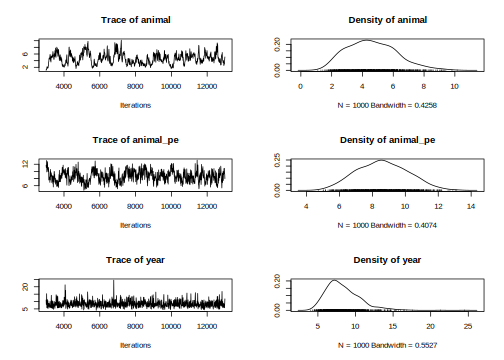
\includegraphics{wam_tuto_files/figure-latex/unnamed-chunk-135-1.pdf} 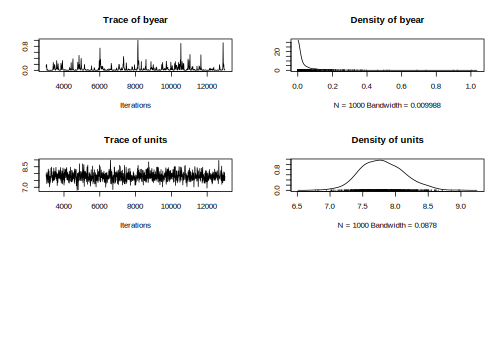
\includegraphics{wam_tuto_files/figure-latex/unnamed-chunk-135-2.pdf}

This model will return additional variance components corresponding to year of measurement effects and birth year (of the female effects) .

\(V_{byear}\) is very low and its posterior distribution (via the function \texttt{HPDinterval} or \texttt{plot}) is very close to zero indicating its not significance. You have to remember bayesien model never estimate variable to 0 or passing zero, so you will never see a credible interval \texttt{CI} crossing zero for a variance.
If you compared the DIC of model3.5 to a reduced model without \texttt{byear}, it should be very similar.

\begin{Shaded}
\begin{Highlighting}[]
\CommentTok{\#p.var \textless{}{-} var(gryphonRM$laydate, na.rm = TRUE)}
\NormalTok{prior3}\FloatTok{.5}\NormalTok{\_}\DecValTok{2}\NormalTok{ \textless{}{-}}\StringTok{ }\KeywordTok{list}\NormalTok{(}\DataTypeTok{G =} \KeywordTok{list}\NormalTok{(}\DataTypeTok{G1 =} \KeywordTok{list}\NormalTok{(}\DataTypeTok{V =} \DecValTok{1}\NormalTok{, }\DataTypeTok{nu =} \FloatTok{0.002}\NormalTok{), }\DataTypeTok{G2 =} \KeywordTok{list}\NormalTok{(}
  \DataTypeTok{V =} \DecValTok{1}\NormalTok{,}
  \DataTypeTok{nu =} \FloatTok{0.002}
\NormalTok{), }\DataTypeTok{G3 =} \KeywordTok{list}\NormalTok{(}\DataTypeTok{V =} \DecValTok{1}\NormalTok{, }\DataTypeTok{nu =} \FloatTok{0.002}\NormalTok{)), }
\DataTypeTok{R =} \KeywordTok{list}\NormalTok{(}\DataTypeTok{V =} \DecValTok{1}\NormalTok{, }\DataTypeTok{nu =} \FloatTok{0.002}\NormalTok{))}

\NormalTok{model3}\FloatTok{.5}\NormalTok{\_}\DecValTok{2}\NormalTok{ \textless{}{-}}\StringTok{ }\KeywordTok{MCMCglmm}\NormalTok{(laydate }\OperatorTok{\textasciitilde{}}\StringTok{ }\DecValTok{1} \OperatorTok{+}\StringTok{ }\NormalTok{age,}
  \DataTypeTok{random =} \OperatorTok{\textasciitilde{}}\StringTok{ }\NormalTok{animal }\OperatorTok{+}\StringTok{ }\NormalTok{animal\_pe }\OperatorTok{+}
\StringTok{    }\NormalTok{year, }\DataTypeTok{ginv =} \KeywordTok{list}\NormalTok{(}\DataTypeTok{animal =}\NormalTok{ Ainv), }\DataTypeTok{data =}\NormalTok{ gryphonRM, }\DataTypeTok{prior =}\NormalTok{ prior3}\FloatTok{.5}\NormalTok{\_}\DecValTok{2}\NormalTok{,}
  \DataTypeTok{verbose =} \OtherTok{FALSE}
\NormalTok{)}
\KeywordTok{posterior.mode}\NormalTok{(model3}\FloatTok{.5}\NormalTok{\_}\DecValTok{2}\OperatorTok{$}\NormalTok{VCV)}
\end{Highlighting}
\end{Shaded}

\begin{verbatim}
##    animal animal_pe      year     units 
##  4.403367  9.243904  7.087309  7.702511
\end{verbatim}

\begin{Shaded}
\begin{Highlighting}[]
\NormalTok{model3}\FloatTok{.5}\OperatorTok{$}\NormalTok{DIC}
\end{Highlighting}
\end{Shaded}

\begin{verbatim}
## [1] 8290.821
\end{verbatim}

\begin{Shaded}
\begin{Highlighting}[]
\NormalTok{model3}\FloatTok{.5}\NormalTok{\_}\DecValTok{2}\OperatorTok{$}\NormalTok{DIC}
\end{Highlighting}
\end{Shaded}

\begin{verbatim}
## [1] 8290.305
\end{verbatim}

\texttt{year} effects could alternatively be included as fixed effects (try it!, you should be able to handle the new prior specification at this point). This will reduce \(V_R\) and increase the estimates of heritability and repeatability, which must now be interpreted as proportions of phenotypic variance after conditioning on both age and year of measurement effects.

\hypertarget{brms-3}{%
\section{brms}\label{brms-3}}

\begin{Shaded}
\begin{Highlighting}[]
\KeywordTok{library}\NormalTok{(brms)}

\NormalTok{Amat \textless{}{-}}\StringTok{ }\KeywordTok{as.matrix}\NormalTok{(nadiv}\OperatorTok{::}\KeywordTok{makeA}\NormalTok{(gryphonped))}
\NormalTok{gryphonRM}\OperatorTok{$}\NormalTok{animal\_pe \textless{}{-}}\StringTok{ }\NormalTok{gryphonRM}\OperatorTok{$}\NormalTok{animal}



\NormalTok{model\_simple1}\FloatTok{.1}\NormalTok{ \textless{}{-}}\StringTok{ }\KeywordTok{brm}\NormalTok{(}
\NormalTok{  laydate }\OperatorTok{\textasciitilde{}}\StringTok{ }\DecValTok{1} \OperatorTok{+}\StringTok{ }\NormalTok{(}\DecValTok{1} \OperatorTok{|}\StringTok{ }\NormalTok{animal) }\OperatorTok{+}\StringTok{ }\NormalTok{(}\DecValTok{1} \OperatorTok{|}\StringTok{ }\NormalTok{animal\_pe),}
  \DataTypeTok{data =}\NormalTok{ gryphonRM,}
  \DataTypeTok{family =} \KeywordTok{gaussian}\NormalTok{(), }\DataTypeTok{data2 =} \KeywordTok{list}\NormalTok{(}\DataTypeTok{Amat =}\NormalTok{ Amat),}
  \DataTypeTok{chains =} \DecValTok{2}\NormalTok{, }\DataTypeTok{cores =} \DecValTok{2}\NormalTok{, }\DataTypeTok{iter =} \DecValTok{1000}
\NormalTok{)}

\KeywordTok{summary}\NormalTok{(model\_simple1}\FloatTok{.1}\NormalTok{)}
\KeywordTok{plot}\NormalTok{(model\_simple1}\FloatTok{.1}\NormalTok{)}
\end{Highlighting}
\end{Shaded}

\hypertarget{stan-2}{%
\section{stan}\label{stan-2}}

to do

\hypertarget{quick-comparison-of-codes}{%
\chapter{Quick comparison of codes}\label{quick-comparison-of-codes}}

\hypertarget{univariate-model-with-repeated-measures}{%
\section{Univariate model with repeated measures}\label{univariate-model-with-repeated-measures}}

\hypertarget{asreml-r-3}{%
\subsection{Asreml-R}\label{asreml-r-3}}

\hypertarget{gremlin-4}{%
\subsection{gremlin}\label{gremlin-4}}

\hypertarget{mcmcglmm-4}{%
\subsection{MCMCglmm}\label{mcmcglmm-4}}

\hypertarget{brms-4}{%
\subsection{brms}\label{brms-4}}

\hypertarget{bivariate-model}{%
\section{bivariate model}\label{bivariate-model}}

\hypertarget{asreml-r-4}{%
\subsection{Asreml-R}\label{asreml-r-4}}

\hypertarget{gremlin-5}{%
\subsection{gremlin}\label{gremlin-5}}

\hypertarget{mcmcglmm-5}{%
\subsection{MCMCglmm}\label{mcmcglmm-5}}

\hypertarget{brms-5}{%
\subsection{brms}\label{brms-5}}

  \bibliography{book.bib,packages.bib}

\printindex

\end{document}
